% Options for packages loaded elsewhere
\PassOptionsToPackage{unicode}{hyperref}
\PassOptionsToPackage{hyphens}{url}
\PassOptionsToPackage{dvipsnames,svgnames,x11names}{xcolor}
%
\documentclass[
  letterpaper,
]{krantz}

\usepackage{amsmath,amssymb}
\usepackage{iftex}
\ifPDFTeX
  \usepackage[T1]{fontenc}
  \usepackage[utf8]{inputenc}
  \usepackage{textcomp} % provide euro and other symbols
\else % if luatex or xetex
  \usepackage{unicode-math}
  \defaultfontfeatures{Scale=MatchLowercase}
  \defaultfontfeatures[\rmfamily]{Ligatures=TeX,Scale=1}
\fi
\usepackage{lmodern}
\ifPDFTeX\else  
    % xetex/luatex font selection
\fi
% Use upquote if available, for straight quotes in verbatim environments
\IfFileExists{upquote.sty}{\usepackage{upquote}}{}
\IfFileExists{microtype.sty}{% use microtype if available
  \usepackage[]{microtype}
  \UseMicrotypeSet[protrusion]{basicmath} % disable protrusion for tt fonts
}{}
\makeatletter
\@ifundefined{KOMAClassName}{% if non-KOMA class
  \IfFileExists{parskip.sty}{%
    \usepackage{parskip}
  }{% else
    \setlength{\parindent}{0pt}
    \setlength{\parskip}{6pt plus 2pt minus 1pt}}
}{% if KOMA class
  \KOMAoptions{parskip=half}}
\makeatother
\usepackage{xcolor}
\usepackage{soul}
\setlength{\emergencystretch}{3em} % prevent overfull lines
\setcounter{secnumdepth}{5}
% Make \paragraph and \subparagraph free-standing
\ifx\paragraph\undefined\else
  \let\oldparagraph\paragraph
  \renewcommand{\paragraph}[1]{\oldparagraph{#1}\mbox{}}
\fi
\ifx\subparagraph\undefined\else
  \let\oldsubparagraph\subparagraph
  \renewcommand{\subparagraph}[1]{\oldsubparagraph{#1}\mbox{}}
\fi

\usepackage{color}
\usepackage{fancyvrb}
\newcommand{\VerbBar}{|}
\newcommand{\VERB}{\Verb[commandchars=\\\{\}]}
\DefineVerbatimEnvironment{Highlighting}{Verbatim}{commandchars=\\\{\}}
% Add ',fontsize=\small' for more characters per line
\usepackage{framed}
\definecolor{shadecolor}{RGB}{241,243,245}
\newenvironment{Shaded}{\begin{snugshade}}{\end{snugshade}}
\newcommand{\AlertTok}[1]{\textcolor[rgb]{0.68,0.00,0.00}{#1}}
\newcommand{\AnnotationTok}[1]{\textcolor[rgb]{0.37,0.37,0.37}{#1}}
\newcommand{\AttributeTok}[1]{\textcolor[rgb]{0.40,0.45,0.13}{#1}}
\newcommand{\BaseNTok}[1]{\textcolor[rgb]{0.68,0.00,0.00}{#1}}
\newcommand{\BuiltInTok}[1]{\textcolor[rgb]{0.00,0.23,0.31}{#1}}
\newcommand{\CharTok}[1]{\textcolor[rgb]{0.13,0.47,0.30}{#1}}
\newcommand{\CommentTok}[1]{\textcolor[rgb]{0.37,0.37,0.37}{#1}}
\newcommand{\CommentVarTok}[1]{\textcolor[rgb]{0.37,0.37,0.37}{\textit{#1}}}
\newcommand{\ConstantTok}[1]{\textcolor[rgb]{0.56,0.35,0.01}{#1}}
\newcommand{\ControlFlowTok}[1]{\textcolor[rgb]{0.00,0.23,0.31}{#1}}
\newcommand{\DataTypeTok}[1]{\textcolor[rgb]{0.68,0.00,0.00}{#1}}
\newcommand{\DecValTok}[1]{\textcolor[rgb]{0.68,0.00,0.00}{#1}}
\newcommand{\DocumentationTok}[1]{\textcolor[rgb]{0.37,0.37,0.37}{\textit{#1}}}
\newcommand{\ErrorTok}[1]{\textcolor[rgb]{0.68,0.00,0.00}{#1}}
\newcommand{\ExtensionTok}[1]{\textcolor[rgb]{0.00,0.23,0.31}{#1}}
\newcommand{\FloatTok}[1]{\textcolor[rgb]{0.68,0.00,0.00}{#1}}
\newcommand{\FunctionTok}[1]{\textcolor[rgb]{0.28,0.35,0.67}{#1}}
\newcommand{\ImportTok}[1]{\textcolor[rgb]{0.00,0.46,0.62}{#1}}
\newcommand{\InformationTok}[1]{\textcolor[rgb]{0.37,0.37,0.37}{#1}}
\newcommand{\KeywordTok}[1]{\textcolor[rgb]{0.00,0.23,0.31}{#1}}
\newcommand{\NormalTok}[1]{\textcolor[rgb]{0.00,0.23,0.31}{#1}}
\newcommand{\OperatorTok}[1]{\textcolor[rgb]{0.37,0.37,0.37}{#1}}
\newcommand{\OtherTok}[1]{\textcolor[rgb]{0.00,0.23,0.31}{#1}}
\newcommand{\PreprocessorTok}[1]{\textcolor[rgb]{0.68,0.00,0.00}{#1}}
\newcommand{\RegionMarkerTok}[1]{\textcolor[rgb]{0.00,0.23,0.31}{#1}}
\newcommand{\SpecialCharTok}[1]{\textcolor[rgb]{0.37,0.37,0.37}{#1}}
\newcommand{\SpecialStringTok}[1]{\textcolor[rgb]{0.13,0.47,0.30}{#1}}
\newcommand{\StringTok}[1]{\textcolor[rgb]{0.13,0.47,0.30}{#1}}
\newcommand{\VariableTok}[1]{\textcolor[rgb]{0.07,0.07,0.07}{#1}}
\newcommand{\VerbatimStringTok}[1]{\textcolor[rgb]{0.13,0.47,0.30}{#1}}
\newcommand{\WarningTok}[1]{\textcolor[rgb]{0.37,0.37,0.37}{\textit{#1}}}

\providecommand{\tightlist}{%
  \setlength{\itemsep}{0pt}\setlength{\parskip}{0pt}}\usepackage{longtable,booktabs,array}
\usepackage{calc} % for calculating minipage widths
% Correct order of tables after \paragraph or \subparagraph
\usepackage{etoolbox}
\makeatletter
\patchcmd\longtable{\par}{\if@noskipsec\mbox{}\fi\par}{}{}
\makeatother
% Allow footnotes in longtable head/foot
\IfFileExists{footnotehyper.sty}{\usepackage{footnotehyper}}{\usepackage{footnote}}
\makesavenoteenv{longtable}
\usepackage{graphicx}
\makeatletter
\def\maxwidth{\ifdim\Gin@nat@width>\linewidth\linewidth\else\Gin@nat@width\fi}
\def\maxheight{\ifdim\Gin@nat@height>\textheight\textheight\else\Gin@nat@height\fi}
\makeatother
% Scale images if necessary, so that they will not overflow the page
% margins by default, and it is still possible to overwrite the defaults
% using explicit options in \includegraphics[width, height, ...]{}
\setkeys{Gin}{width=\maxwidth,height=\maxheight,keepaspectratio}
% Set default figure placement to htbp
\makeatletter
\def\fps@figure{htbp}
\makeatother
\newlength{\cslhangindent}
\setlength{\cslhangindent}{1.5em}
\newlength{\csllabelwidth}
\setlength{\csllabelwidth}{3em}
\newlength{\cslentryspacingunit} % times entry-spacing
\setlength{\cslentryspacingunit}{\parskip}
\newenvironment{CSLReferences}[2] % #1 hanging-ident, #2 entry spacing
 {% don't indent paragraphs
  \setlength{\parindent}{0pt}
  % turn on hanging indent if param 1 is 1
  \ifodd #1
  \let\oldpar\par
  \def\par{\hangindent=\cslhangindent\oldpar}
  \fi
  % set entry spacing
  \setlength{\parskip}{#2\cslentryspacingunit}
 }%
 {}
\usepackage{calc}
\newcommand{\CSLBlock}[1]{#1\hfill\break}
\newcommand{\CSLLeftMargin}[1]{\parbox[t]{\csllabelwidth}{#1}}
\newcommand{\CSLRightInline}[1]{\parbox[t]{\linewidth - \csllabelwidth}{#1}\break}
\newcommand{\CSLIndent}[1]{\hspace{\cslhangindent}#1}

\usepackage{booktabs}
\usepackage{longtable}
\usepackage[bf,singlelinecheck=off]{caption}
\usepackage{url}

\usepackage{framed,color}
\definecolor{shadecolor}{RGB}{248,248,248}

\renewcommand{\textfraction}{0.05}
\renewcommand{\topfraction}{0.8}
\renewcommand{\bottomfraction}{0.8}
\renewcommand{\floatpagefraction}{0.75}

\renewenvironment{quote}{\begin{VF}}{\end{VF}}
\let\oldhref\href
\providecommand{\href}[2]{#2\footnote{\url{#1}}}
  
\makeatletter
\newenvironment{kframe}{%
  \medskip{}
  \setlength{\fboxsep}{.8em}
  \def\at@end@of@kframe{}%
  \ifinner\ifhmode%
  \def\at@end@of@kframe{\end{minipage}}%
  \begin{minipage}{\columnwidth}%
  \fi\fi%
  \def\FrameCommand##1{\hskip\@totalleftmargin \hskip-\fboxsep
  \colorbox{shadecolor}{##1}\hskip-\fboxsep
    % There is no \\@totalrightmargin, so:
      \hskip-\linewidth \hskip-\@totalleftmargin \hskip\columnwidth}%
  \MakeFramed {\advance\hsize-\width
    \@totalleftmargin\z@ \linewidth\hsize
    \@setminipage}}%
{\par\unskip\endMakeFramed%
  \at@end@of@kframe}
\makeatother

\renewenvironment{Shaded}{\begin{kframe}}{\end{kframe}}

\usepackage{makeidx}
\makeindex

\urlstyle{tt}

\usepackage{amsthm}
\makeatletter
\def\thm@space@setup{%
  \thm@preskip=8pt plus 2pt minus 4pt
  \thm@postskip=\thm@preskip
}
\makeatother

\frontmatter
  
  
\makeatletter
\@ifpackageloaded{tcolorbox}{}{\usepackage[skins,breakable]{tcolorbox}}
\@ifpackageloaded{fontawesome5}{}{\usepackage{fontawesome5}}
\definecolor{quarto-callout-color}{HTML}{909090}
\definecolor{quarto-callout-note-color}{HTML}{0758E5}
\definecolor{quarto-callout-important-color}{HTML}{CC1914}
\definecolor{quarto-callout-warning-color}{HTML}{EB9113}
\definecolor{quarto-callout-tip-color}{HTML}{00A047}
\definecolor{quarto-callout-caution-color}{HTML}{FC5300}
\definecolor{quarto-callout-color-frame}{HTML}{acacac}
\definecolor{quarto-callout-note-color-frame}{HTML}{4582ec}
\definecolor{quarto-callout-important-color-frame}{HTML}{d9534f}
\definecolor{quarto-callout-warning-color-frame}{HTML}{f0ad4e}
\definecolor{quarto-callout-tip-color-frame}{HTML}{02b875}
\definecolor{quarto-callout-caution-color-frame}{HTML}{fd7e14}
\makeatother
\makeatletter
\makeatother
\makeatletter
\@ifpackageloaded{bookmark}{}{\usepackage{bookmark}}
\makeatother
\makeatletter
\@ifpackageloaded{caption}{}{\usepackage{caption}}
\AtBeginDocument{%
\ifdefined\contentsname
  \renewcommand*\contentsname{Table of contents}
\else
  \newcommand\contentsname{Table of contents}
\fi
\ifdefined\listfigurename
  \renewcommand*\listfigurename{List of Figures}
\else
  \newcommand\listfigurename{List of Figures}
\fi
\ifdefined\listtablename
  \renewcommand*\listtablename{List of Tables}
\else
  \newcommand\listtablename{List of Tables}
\fi
\ifdefined\figurename
  \renewcommand*\figurename{Figure}
\else
  \newcommand\figurename{Figure}
\fi
\ifdefined\tablename
  \renewcommand*\tablename{Table}
\else
  \newcommand\tablename{Table}
\fi
}
\@ifpackageloaded{float}{}{\usepackage{float}}
\floatstyle{ruled}
\@ifundefined{c@chapter}{\newfloat{codelisting}{h}{lop}}{\newfloat{codelisting}{h}{lop}[chapter]}
\floatname{codelisting}{Listing}
\newcommand*\listoflistings{\listof{codelisting}{List of Listings}}
\makeatother
\makeatletter
\@ifpackageloaded{caption}{}{\usepackage{caption}}
\@ifpackageloaded{subcaption}{}{\usepackage{subcaption}}
\makeatother
\makeatletter
\@ifpackageloaded{tcolorbox}{}{\usepackage[skins,breakable]{tcolorbox}}
\makeatother
\makeatletter
\@ifundefined{shadecolor}{\definecolor{shadecolor}{rgb}{.97, .97, .97}}
\makeatother
\makeatletter
\makeatother
\makeatletter
\@ifpackageloaded{sidenotes}{}{\usepackage{sidenotes}}
\@ifpackageloaded{marginnote}{}{\usepackage{marginnote}}
\makeatother
\makeatletter
\makeatother
\ifLuaTeX
  \usepackage{selnolig}  % disable illegal ligatures
\fi
\IfFileExists{bookmark.sty}{\usepackage{bookmark}}{\usepackage{hyperref}}
\IfFileExists{xurl.sty}{\usepackage{xurl}}{} % add URL line breaks if available
\urlstyle{same} % disable monospaced font for URLs
\hypersetup{
  pdftitle={Visualizing Multivariate Data and Models in R},
  pdfauthor={Michael Friendly},
  colorlinks=true,
  linkcolor={blue},
  filecolor={Maroon},
  citecolor={Blue},
  urlcolor={Blue},
  pdfcreator={LaTeX via pandoc}}

\title{Visualizing Multivariate Data and Models in R}
\usepackage{etoolbox}
\makeatletter
\providecommand{\subtitle}[1]{% add subtitle to \maketitle
  \apptocmd{\@title}{\par {\large #1 \par}}{}{}
}
\makeatother
\subtitle{A Romance in Many Dimensions}
\author{Michael Friendly}
\date{2024-01-01}

\begin{document}
\maketitle
% you may need to leave a few empty pages before the dedication page

%\cleardoublepage\newpage\thispagestyle{empty}\null
%\cleardoublepage\newpage\thispagestyle{empty}\null
%\cleardoublepage\newpage
\thispagestyle{empty}

\begin{center}
To all the mistakes I've made (data, and otherwise) and those who tolerated my making them.
%\includegraphics{images/dedication.pdf}
\end{center}

\setlength{\abovedisplayskip}{-5pt}
\setlength{\abovedisplayshortskip}{-5pt}

\ifdefined\Shaded\renewenvironment{Shaded}{\begin{tcolorbox}[enhanced, breakable, interior hidden, frame hidden, borderline west={3pt}{0pt}{shadecolor}, boxrule=0pt, sharp corners]}{\end{tcolorbox}}\fi

\renewcommand*\contentsname{Table of contents}
{
\hypersetup{linkcolor=}
\setcounter{tocdepth}{2}
\tableofcontents
}
\bookmarksetup{startatroot}

\hypertarget{preface}{%
\chapter*{Preface}\label{preface}}
\addcontentsline{toc}{chapter}{Preface}

\markboth{Preface}{Preface}

\textbf{TODO}: Make this a more general introduction\\
This book is about graphical methods developed recently for multivariate
data, and their uses in understanding relationships when there are
several aspects to be considered together. Data visualization methods
for statistical analysis are well-developed for simple linear models
with a single outcome variable. However, with applied research in the
social and behavioral sciences, it is often the case that the phenomena
of interest (e.g., depression, job satisfaction, academic achievement,
childhood ADHD disorders, etc.) can be measured in several different
ways or related aspects.

For example, if academic achievement can be measured for adolescents by
reading, mathematics, science and history scores, how do predictors such
as parental encouragement, school environment and socioeconomic status
affect all these outcomes? In a similar way? In different ways? In such
cases, much more can be understood from a multivariate approach that
considers the correlations among the outcomes. Yet, sadly, researchers
typically examine the outcomes one by one which often only tells part of
the data story.

However, to do this it is useful to set the stage for multivariate
thinking, with a grand scheme for statistics and data visualization, a
parable, and an example of multivariate discovery.

\hypertarget{one-two-many}{%
\section*{ONE, TWO, MANY}\label{one-two-many}}
\addcontentsline{toc}{section}{ONE, TWO, MANY}

\markright{ONE, TWO, MANY}

There is an old and helpful idea I learned from John Hartigan in my
graduate days at Princeton:

\begin{quote}
In statistics and data visualization \emph{all} methods can be
classified by the number of dimensions contemplated, on a scale of
\textbf{ONE}, \textbf{TWO}, \textbf{MANY}.
\end{quote}

By this, he meant that, at a global level, all data, statistical
summaries, and graphical displays could be classified as:

\begin{itemize}
\tightlist
\item
  \textbf{univariate}: a single variable, considered in isolation (age,
  COVID cases, pizzas ordered). Univariate numerical summaries are
  means, medians, measures of variablilty, and so forth. Univariate
  displays include dot plots, boxplots, histograms and density
  estimates.
\item
  \textbf{bivariate}: two variables, considered jointly. Numerical
  summaries include correlations, covariances and two-way tables of
  frequencies or measures of association for categorical variables.
  Bivariate displays include scatterplots and mosaic plots.
\item
  \textbf{multivariate}: three or more variables, considered jointly.
  Numerical summaries include correlation and covariance matrices,
  consisting of all pairwise values, but also derived measures from the
  analysis of these matrices (eigenvalues, eigenvectors). Graphical
  displays of multivariate data can sometimes be shown in 3D, but often
  involve multiple views of the data projected into 2D plots.
\end{itemize}

As a quasi-numerical scale, I refer to these as \textbf{1D}, \textbf{2D}
and \textbf{nD}. This admits the possibility of half-integer cases, such
as \textbf{1.5D}, where the main focus is on a single variable, but that
is classified by a simple factor (e.g., gender), or \textbf{2.5D} where
a 2D scatterplot can show other variables using color, shape or other
visual attributes His point in this classification was that once you've
reached three variables, all higher dimensions involve similar summaries
and data displays.

Univariate and bivariate methods and displays are well-known. This book
is about how these ideas can be extended to an \(n\)-dimensional world.
Three-dimensional data displays are now fairly easy to produce, even if
they are sometimes difficult to understand. But how can we even think
about four or more dimensions? The difficulty can be appreciated by
considering the tale of \emph{Flatland}.

\hypertarget{flatland}{%
\section*{Flatland}\label{flatland}}
\addcontentsline{toc}{section}{Flatland}

\markright{Flatland}

\begin{quote}
To comport oneself with perfect propriety in Polygonal society, one
ought to be a Polygon oneself. --- Edwin A. Abbott, \emph{Flatland}
\end{quote}

In 1884, an English schoolmaster, Edwin Abbott Abbott, shook the world
of Victorian culture with a slim volume, \emph{Flatland: A Romance of
Many Dimensions} (\protect\hyperlink{ref-Abbott:1884}{Abbott, 1884}). He
described a two-dimensional world, \emph{Flatland}, inhabited entirely
by geometric figures in the plane. His purpose was satirical, to poke
fun at the social and gender class system at the time: Women were mere
line segments, while men were represented as polygons with varying
numbers of sides--- a triangle was a working man, but acute isosceles
were soldiers or criminals of very small angle; gentlemen and
professionals had more sides. Abbot published this under the pseudonym,
``A Square'', suggesting his place in the hierarchy.

\begin{quote}
True, said the Sphere; it appears to you a Plane, because you are not
accustomed to light and shade and perspective; just as in Flatland a
Hexagon would appear a Straight Line to one who has not the Art of Sight
Recognition. But in reality it is a Solid, as you shall learn by the
sense of Feeling. --- Edwin A. Abbott, \emph{Flatland}
\end{quote}

But how did it feel to be a member of a flatland society? How could a
point (a newborn child?) understand a line (a woman)? How does a
Triangle ``see'' a Hexagon or even a infinitely-sided Circle? Abbott
introduces the very idea of different dimensions of existence through
dreams and visions:

\begin{itemize}
\item
  A Square dreams of visiting a one-dimensional \emph{Lineland} where
  men appear as lines, and women are merely ``illustrious points'', but
  the inhabitants can only see the Square as lines.
\item
  In a vision, the Square is visited by a Sphere, to illustrate what a
  2D Flatlander could understand from a 3D sphere
  (Figure~\ref{fig-flatland-spheres}) that passes through the plane he
  inhabits. It is a large circle when seen at the moment of its'
  greatest extent. As the Spehere rises, it becomes progressively
  smaller, until it becomes a point, and then vanishes.
\end{itemize}

\begin{figure}

{\centering 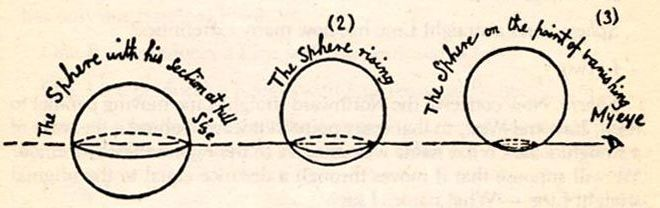
\includegraphics[width=0.9\textwidth,height=\textheight]{images/flatland-spheres.jpg}

}

\caption{\label{fig-flatland-spheres}A 2D Flatlander seeing a sphere as
it passes through Flatland. The line, labeled `My Eye' indicates what
the Flatlander would see. Source: Abbott
(\protect\hyperlink{ref-Abbott:1884}{1884})}

\end{figure}

Abbott goes on to state what could be considered as a demonstration (or
proof) by induction of the difficulties of seeing in 1, 2, 3 dimensions,
and how the idea motion over time (one more dimension) could allow
citizens of any 1D, 2D, 3D world to contemplate one more dimension.

\begin{quote}
In One Dimensions, did not a moving Point produce a Line with two
terminal points? In two Dimensions, did not a moving Line produce a
Square with four terminal points? In Three Dimensions, did not a moving
Square produce - did not the eyes of mine behold it - that blessed
being, a Cube, with eight terminal points? And in Four Dimensions, shall
not a moving Cube - alas, for Analogy, and alas for the Progress of
Truth if it be not so - shall not, I say the motion of a divine Cube
result in a still more divine organization with sixteen terminal points?
--- Edwin A. Abbott
\end{quote}

For Abbot, the way for a citizen of any world to imagine one more
dimension was to consider how a higher-dimensional object would change
over time.\footnote{In his famous TV series, \emph{Cosmos}, Carl Sagan
  provides \href{https://youtu.be/UnURElCzGc0}{an intriguing video
  presentation} Flatland and the 4th dimension. However, as far back as
  1754 (\protect\hyperlink{ref-Cajori:1926}{Cajori, 1926}), the idea of
  adding a fourth dimension appears in Jean le Rond d'Alembert's
  ``Dimensions'', and one realization of a four-dimensional object is a
  \emph{tesseract}, shown in Figure~\ref{fig-1D-4D}.} A line moved over
time could produce a rectangle as shown in Figure~\ref{fig-1D-4D}; that
rectangle moving in another direction over time would produce a 3D
figure, and so forth.

\begin{figure}

{\centering 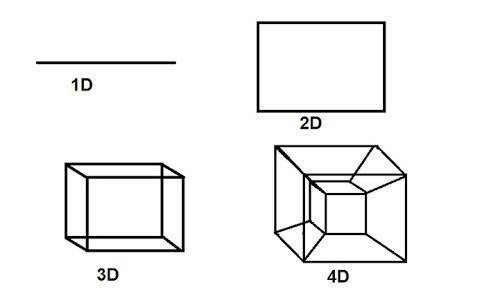
\includegraphics[width=0.9\textwidth,height=\textheight]{images/1D-4D.png}

}

\caption{\label{fig-1D-4D}Geometrical objects in 1 to 4 dimensions. One
more dimension can be thought of as the trace of movement over time.}

\end{figure}

But wait! Where does that 4D thing (a \emph{tesseract}) come from? To
really see a tesseract it helps to view it in an animation over time.
But like the Square, contemplating 3D from a 2D world, it takes some
imagination.

\begin{figure}

{\centering 

}

\caption{\label{fig-tesseract}Animation of a tesseract, a cube changing
over time.}

\end{figure}

Yet the deep mathematics of more than three dimensions only emerged in
the 19th century. In Newtonian mechanics, space and time were always
considered independent of each other. Our familiar three-dimensional
space, of length, width, and height had formed the backbone of Euclidean
geometry for millenea. However, the idea that space and time are indeed
interwoven was first proposed by German mathematician Hermann Minkowski
(1864--1909) in 1908. This was a powerful idea. It bore fruit when
Albert Einstein revolutionized the Newtonian conceptions of gravity in
1915 when he presented a theory of general relativity which was based
primarily on the fact that mass and energy warp the fabric of
four-dimensional spacetime.

The parable of \emph{Flatland} can provide inspiration for statistical
thinking and data visualization. Once we go beyond bivariate statistics
and 2D plots, we are in a multivariate world of possibly MANY
dimensions. It takes only some imagination and suitable methods to get
there.

Like Abbott's \emph{Flatland}, this book is a romance, in many
dimensions, of what we can learn from modern methods of data
visualization.

\hypertarget{eureka}{%
\section*{EUREKA!}\label{eureka}}
\addcontentsline{toc}{section}{EUREKA!}

\markright{EUREKA!}

Even modest sized multivariate data can have secrets that can be
revealed in the right view. As an example, David Coleman at RCA
Laboratories in Princeton, N.J. generated a dataset of five (fictitious)
measurements of grains of pollen for the 1986 Data Exposition at the
Joint statistical Meetings. The first three variables are the lengths of
geometric features 3848 observed sampled pollen grains -- in the x, y,
and z dimensions: a \texttt{ridge} along x, a \texttt{nub} in the y
direction, and a \texttt{crack} in along the z dimension. The fourth
variable is pollen grain \texttt{weight}, and the fifth is
\texttt{density}. The challenge was to ``find something interesting'' in
this dataset.

Those who solved the puzzle were able to find an orientation of this
5-dimensional dataset, such that zooming in revealed a magic word,
``EUREKA'' spelled in points, as in the following figure.

\begin{figure}

\begin{minipage}[t]{0.50\linewidth}

{\centering 

\raisebox{-\height}{

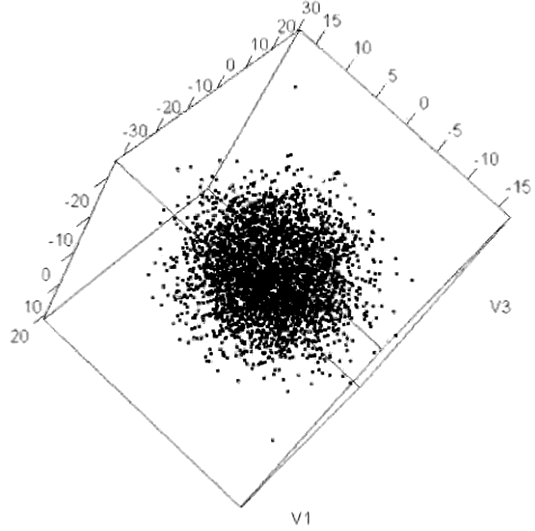
\includegraphics{images/pollen-eureka1.png}

}

}

\end{minipage}%
%
\begin{minipage}[t]{0.50\linewidth}

{\centering 

\raisebox{-\height}{

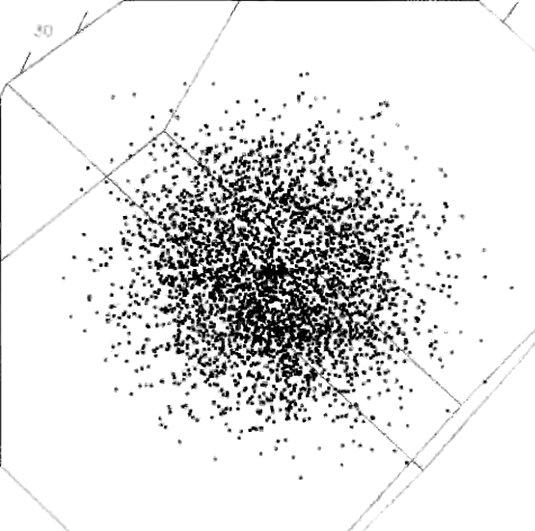
\includegraphics{images/pollen-eureka2.png}

}

}

\end{minipage}%
\newline
\begin{minipage}[t]{0.50\linewidth}

{\centering 

\raisebox{-\height}{

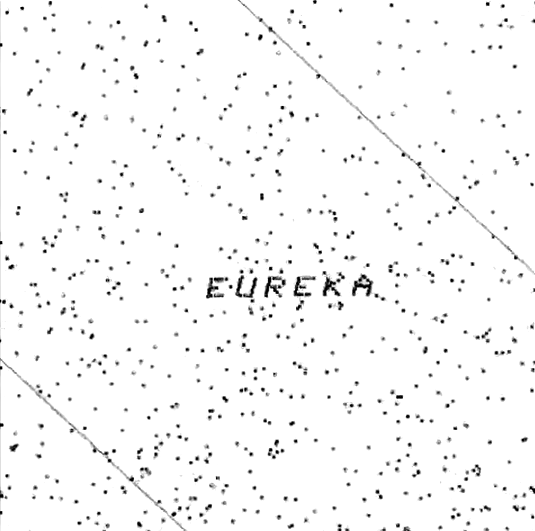
\includegraphics{images/pollen-eureka4.png}

}

}

\end{minipage}%
%
\begin{minipage}[t]{0.50\linewidth}

{\centering 

\raisebox{-\height}{

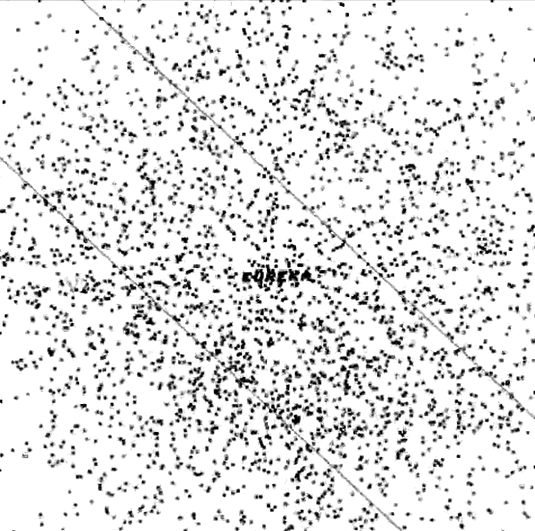
\includegraphics{images/pollen-eureka3.png}

}

}

\end{minipage}%

\caption{\label{fig-pollen-eureka}Four views of the \texttt{pollen}
data, zooming in, clockwise from the upper left to discover the word
``EUREKA''.}

\end{figure}

This can be seen better in a 3D animation. \texttt{rgl}
(\protect\hyperlink{ref-R-rgl}{Adler \& Murdoch, 2023}) is used to
create a 3D scatterplot of the first three variables. Then the
\texttt{animation} package (\protect\hyperlink{ref-R-animation}{Xie,
2021}) is use to record a sequence of images, adjusting the
\texttt{rgl::par3d(zoom)} value.

\begin{Shaded}
\begin{Highlighting}[]
\FunctionTok{library}\NormalTok{(animation)}
\FunctionTok{library}\NormalTok{(rgl)}
\FunctionTok{data}\NormalTok{(pollen, }\AttributeTok{package =} \StringTok{"animation"}\NormalTok{)}
\NormalTok{oopt }\OtherTok{=} \FunctionTok{ani.options}\NormalTok{(}\AttributeTok{interval =} \FloatTok{0.05}\NormalTok{)}
\DocumentationTok{\#\# adjust the viewpoint}
\NormalTok{uM }\OtherTok{=}
  \FunctionTok{matrix}\NormalTok{(}\FunctionTok{c}\NormalTok{(}\SpecialCharTok{{-}}\FloatTok{0.370919227600098}\NormalTok{, }\SpecialCharTok{{-}}\FloatTok{0.513357102870941}\NormalTok{,}
           \SpecialCharTok{{-}}\FloatTok{0.773877620697021}\NormalTok{, }\DecValTok{0}\NormalTok{, }\SpecialCharTok{{-}}\FloatTok{0.73050606250763}\NormalTok{, }\FloatTok{0.675815105438232}\NormalTok{,}
           \SpecialCharTok{{-}}\FloatTok{0.0981751680374146}\NormalTok{, }\DecValTok{0}\NormalTok{, }\FloatTok{0.573396027088165}\NormalTok{, }\FloatTok{0.528906404972076}\NormalTok{,}
           \SpecialCharTok{{-}}\FloatTok{0.625681936740875}\NormalTok{, }\DecValTok{0}\NormalTok{, }\DecValTok{0}\NormalTok{, }\DecValTok{0}\NormalTok{, }\DecValTok{0}\NormalTok{, }\DecValTok{1}\NormalTok{), }\DecValTok{4}\NormalTok{, }\DecValTok{4}\NormalTok{)}
\FunctionTok{open3d}\NormalTok{(}\AttributeTok{userMatrix =}\NormalTok{ uM, }
       \AttributeTok{windowRect =} \FunctionTok{c}\NormalTok{(}\DecValTok{10}\NormalTok{, }\DecValTok{10}\NormalTok{, }\DecValTok{510}\NormalTok{, }\DecValTok{510}\NormalTok{))}

\FunctionTok{plot3d}\NormalTok{(pollen[, }\DecValTok{1}\SpecialCharTok{:}\DecValTok{3}\NormalTok{])}

\CommentTok{\# zoom in}
\NormalTok{zm }\OtherTok{=} \FunctionTok{seq}\NormalTok{(}\DecValTok{1}\NormalTok{, }\FloatTok{0.045}\NormalTok{, }\AttributeTok{length =} \DecValTok{200}\NormalTok{)}
\FunctionTok{par3d}\NormalTok{(}\AttributeTok{zoom =} \DecValTok{1}\NormalTok{)}
\ControlFlowTok{for}\NormalTok{ (i }\ControlFlowTok{in} \DecValTok{1}\SpecialCharTok{:}\FunctionTok{length}\NormalTok{(zm)) \{}
  \FunctionTok{par3d}\NormalTok{(}\AttributeTok{zoom =}\NormalTok{ zm[i])}
  \FunctionTok{ani.pause}\NormalTok{()}
\NormalTok{\}}
\FunctionTok{ani.options}\NormalTok{(oopt)}
\end{Highlighting}
\end{Shaded}

\begin{figure}

{\centering 

}

\caption{\label{fig-pollen-eureka-fig}Animation of zooming in on the
\texttt{pollen} data.}

\end{figure}

Lest this example seem contrived (which it admittedly is), multivariate
visualization has played an important role in quite a few scientific
discoveries. Among these \textbf{TODO} \ldots{} diabetes classification
\ldots.

\hypertarget{what-i-assume}{%
\section*{What I assume}\label{what-i-assume}}
\addcontentsline{toc}{section}{What I assume}

\markright{What I assume}

It is assumed that the reader has a background in intermediate
statistics including material on univariate linear models including
analysis of variance (ANOVA) and multiple regression. This means you
should be familiar with \ldots{}

There will also be some mathematics in the book where words and diagrams
are not enough. The mathematical level will be intermediate, mostly
consisting of simple algebra. No derivations, proofs, theorems here! For
multivariate methods, it will be useful to express ideas using matrix
notation to simplify presentation. I'm using math to express ideas, and
all you will need is a reading-level of understanding.

I also assume the reader to have at least a basic familiarity with R.
While R fundamentals are outside the scope of the book, I believe that
this language provides a rich set of resources, far beyond that offered
by other statistical software packages, and is well worth learning.

For those not familiar with R, I recommend Matloff
(\protect\hyperlink{ref-Matloff-2011}{2011}), Wickham
(\protect\hyperlink{ref-Wickham2014}{2014}), and Cotton
(\protect\hyperlink{ref-Cotton-2013}{2013}) for introductions to
programming in the language, and Fox \& Weisberg
(\protect\hyperlink{ref-FoxWeisberg:2018}{2018}) and Teetor
(\protect\hyperlink{ref-Teetor2011}{2011}) for learning about how to
conduct basic statistical analyses. \textbf{TODO}: Revise this list.

\hypertarget{conventions-used-in-this-book}{%
\section*{Conventions used in this
book}\label{conventions-used-in-this-book}}
\addcontentsline{toc}{section}{Conventions used in this book}

\markright{Conventions used in this book}

The following typographic conventions are used in this book:

\begin{itemize}
\item
  \emph{italic} : indicates terms to be \emph{emphasized} or defined in
  the text, \ldots{}
\item
  \textbf{bold} : is used for names of R packages
\item
  \texttt{fixed-width} : is used in program listings as well as in text
  to refer to variable and function names, R statement elements and
  keywords.
\item
  \emph{\texttt{fixed-width\ italic}} : isn't used yet, but probably
  should be.
\end{itemize}

For R functions in packages, we use the notation
\texttt{package::function()}, for example: \texttt{car::Anova()} to
identify where those functions are defined

\bookmarksetup{startatroot}

\hypertarget{sec-introduction}{%
\chapter{Introduction}\label{sec-introduction}}

This material may or may not survive; it was taken from an earlier
article.

\hypertarget{multivariate-vs.-multivariable-methods}{%
\section{Multivariate vs.~multivariable
methods}\label{multivariate-vs.-multivariable-methods}}

\begin{quote}
multivariate \(\ne\) multivariable
\end{quote}

In this era of multivitamins, multitools, multifactor authentication and
even the multiverse, it is well to understand the distinction between
\emph{multivariate} and \emph{multivariable} methods as these terms are
generally used and as I use them here in relation to statistical methods
and data visualization. The distinction is simple:

\begin{itemize}
\item
  \textbf{Multivariate methods} for linear models such as multivariate
  regression have more than one dependent, response or outcome variable.
  Other multivariate methods such as principal components analysis or
  factor analysis treat all variables on an equal footing.
\item
  \textbf{Multivariable methods} have a single dependent variable and
  more than one independent variables or covariates.
\end{itemize}

\hypertarget{why-use-a-multivariate-design}{%
\section{Why use a multivariate
design}\label{why-use-a-multivariate-design}}

A particular research outcome (e.g., depression, neuro-cognitive
functioning, academic achievement, self-concept, attention deficit
hyperactivity disorders) might take on a multivariate form if it has
several observed measurement scales or related aspects by which it is
quantified, or if there are multiple theoretically distinct outcomes
that should be assessed in conjunction with each other (e.g., using
depression, generalized anxiety, and stress inventories to model overall
happiness). In this situation, the primary concern of the researcher is
to ascertain the impact of potential predictors on two or more response
variables simultaneously.

For example, if academic achievement is measured for adolescents by
their reading, mathematics, science, and history scores, the following
questions are of interest:

\begin{itemize}
\item
  Do predictors such as parent encouragement, socioeconomic status and
  school environmental variables affect \emph{all} of these outcomes?
\item
  Do they affect them in the \emph{same} or \emph{different} ways?
\item
  How many different aspects of academic achievement can be
  distinguished in the predictors? Equivalently, is academic achievement
  \emph{unidimensional} or \emph{multidimensional} in relation to the
  predictors?
\end{itemize}

Similarly, if psychiatric patients in various diagnostic categories are
measured on a battery of tests related to social skills and cognitive
functioning, we might want to know:

\begin{itemize}
\item
  Which measures best discriminate among the diagnostic groups?
\item
  Which measures are most predictive of positive outcomes?
\item
  Further, how are the \emph{relationships} between the outcomes
  affected by the predictors?
\end{itemize}

Such questions obviously concern more than just the separate univariate
relations of each response to the predictors. Equally, or perhaps more
importantly, are questions of how the response variables are predicted
\emph{jointly}.

\begin{tcolorbox}[enhanced jigsaw, colback=white, rightrule=.15mm, left=2mm, arc=.35mm, colframe=quarto-callout-note-color-frame, toptitle=1mm, breakable, leftrule=.75mm, opacityback=0, bottomtitle=1mm, colbacktitle=quarto-callout-note-color!10!white, opacitybacktitle=0.6, titlerule=0mm, toprule=.15mm, title=\textcolor{quarto-callout-note-color}{\faInfo}\hspace{0.5em}{SEM}, bottomrule=.15mm, coltitle=black]

Structural equation modeling (SEM) offers another route to explore and
analyze the relationships among multiple predictors and multiple
responses. They have the advantage of being able to test potentially
complex systems of linear equations in very flexible ways; however,
these methods are often far removed from data analysis \emph{per se} and
except for path diagrams offer little in the way of visualization
methods to aid in understanding and communicating the results. The
graphical methods we describe here can also be useful in a SEM context.

\end{tcolorbox}

\hypertarget{linear-models-univariate-to-multivariate}{%
\section{Linear models: Univariate to
multivariate}\label{linear-models-univariate-to-multivariate}}

For classical linear models for ANOVA and regression, the step from a
univariate model for a single response, \(y\), to a multivariate one for
a collection of \(p\) responses, \(\mathbf{y}\) is conceptually very
easy. That's because the univariate model,

\[y_i = \beta_0 + \beta_1 x_1 + \beta_2 x_2 + \dots + \beta_q x_q + u_i , \]

or, in matrix terms,

\[\mathbf{y} = \mathbf{X} \; \mathbf{\beta} + \mathbf{u}, \quad\mbox{   with   }\quad \mathbf{u} \sim \mathcal{N} (0, \sigma^2 \mathbf{I}) ,\]

generalizes directly to an analogous multivariate linear model (MLM),

\[\mathbf{Y} = [\mathbf{y_1}, \mathbf{y_2}, \dots, \mathbf{y_p}] = \mathbf{X} \; \mathbf{B} + \mathbf{U} \quad\mbox{   with   }\quad \mathbf{U} \sim \mathcal{N} (\mathbf{0}, \mathbf{\Sigma})\]

for multiple responses (as will be discussed in detail). The design
matrix, \(\mathbf{X}\) remains the same, and the vector \(\beta\) of
coefficients becomes a matrix \(\mathbf{B}\), with one column for each
of the \(p\) outcome variables.

Happily as well, hypothesis tests for the MLM are also straight-forward
generalizations of the familiar \(F\) and \(t\)-tests for univariate
response models. Moreover, there is a rich geometry underlying these
generalizations which we can exploit for understanding and
visualization.

\hypertarget{visualization-is-harder}{%
\section{Visualization is harder}\label{visualization-is-harder}}

However, with two or more response variables, visualizations for
multivariate models are not as simple as they are for their univariate
counterparts for understanding the effects of predictors, model
parameters, or model diagnostics. Consequently, the results of such
studies are often explored and discussed solely in terms of coefficients
and significance, and visualizations of the relationships are only
provided for one response variable at a time, if at all. This tradition
can mask important nuances, and lead researchers to draw erroneous
conclusions.

The aim of this book is to describe and illustrate some central methods
that we have developed over the last ten years that aid in the
understanding and communication of the results of multivariate linear
models (\protect\hyperlink{ref-Friendly-07-manova}{Friendly, 2007};
\protect\hyperlink{ref-FriendlyMeyer:2016:DDAR}{Friendly \& Meyer,
2016}). These methods rely on \emph{data ellipsoids} as simple,
minimally sufficient visualizations of variance that can be shown in 2D
and 3D plots. As will be demonstrated, the \emph{Hypothesis-Error (HE)
plot} framework applies this idea to the results of multivariate tests
of linear hypotheses.

Further, in the case where there are more than just a few outcome
variables, the important nectar of their relationships to predictors can
often be distilled in a multivariate juicer--- a \textbf{projection} of
the multivariate relationships to the predictors in the low-D space that
captures most of the flavor. This idea can be applied using
\emph{canonical correlation plots} and with \emph{canonical discriminant
HE plots}.

\begin{figure}

{\centering 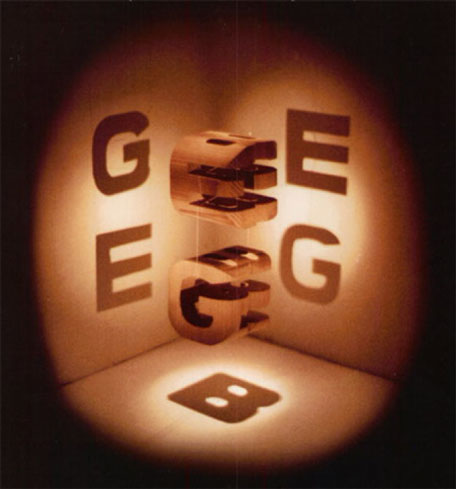
\includegraphics{images/Cover-image-GBE.png}

}

\caption{\textbf{Projection}: The cover image from Hofstadter's
\emph{Goedel, Bach and Escher} illustrates projection of 3D solids onto
each 2D plane.}

\end{figure}

\hypertarget{sec-problems}{%
\section{Problems in understanding and communicating MLM
results}\label{sec-problems}}

In my consulting practice within the Statistical Consulting Service at
York University, I see hundreds of clients each year ranging from
advanced undergraduate thesis students, to graduate students and faculty
from a variety of fields. Over the last two decades, and across each of
these groups, I have noticed an increasing desire to utilize
multivariate methods. As researchers are exposed to the utility and
power of multivariate tests, they see them as an appealing alternative
to running many univariate ANOVAs or multiple regressions for each
response variable separately.

However, multivariate analyses are more complicated than such
approaches, especially when it comes to understanding and communicating
results. Output is typically voluminous, and researchers will often get
lost in the numbers. While software (SPSS, SAS and R) make tabular
summary displays easy, these often obscure the findings that researchers
are most interested in. The most common analytic oversights that we have
observed are:

\begin{itemize}
\item
  \textbf{Atomistic data screening}: Researchers have mostly learned the
  assumptions (the Holy Trinity of normality, constant variance and
  independence) of univariate linear models, but then apply
  \emph{univariate} tests (e.g., Shapiro-Wilk) and diagnostic plots
  (normal QQ plots) to every predictor and every response.
\item
  \textbf{Bonferroni everywhere}: Faced with the task of reporting the
  results for multiple response measures and a collection of predictors
  for each, a common tendency is to run (and sometimes report) each of
  the separate univariate response models and then apply a correction
  for multiple testing. Not only is this confusing and awkward to
  report, but it is largely unnecessary because the multivariate tests
  provide protection for multiple testing.
\item
  \textbf{Reverting to univariate visualizations}: To display results,
  SPSS and SAS make some visualization methods available through menu
  choices or syntax, but usually these are the wrong (or at least
  unhelpful) choices, in that they generate separate univariate graphs
  for the individual responses.
\end{itemize}

This book to discusses a few essential procedures for multivariate
linear models, how their interpretation can be aided through the use of
well-crafted (though novel) visualizations, and provides replicable
sample code in R to showcase their use in applied behaviorial research.
A later section {[}ref?{]} provides some practical guidelines for
analyzing, visualizing and reporting such models to help avoid these and
other problems.

\begin{Shaded}
\begin{Highlighting}[]
\CommentTok{\#cat("Packages used here:\textbackslash{}n")}
\FunctionTok{write\_pkgs}\NormalTok{(}\AttributeTok{file =}\NormalTok{ .pkg\_file)}
\CommentTok{\#\textgreater{} 8  packages used here:}
\CommentTok{\#\textgreater{}  base, datasets, graphics, grDevices, knitr, methods, stats, utils}
\end{Highlighting}
\end{Shaded}

\bookmarksetup{startatroot}

\hypertarget{sec-getting_started}{%
\chapter{Getting Started}\label{sec-getting_started}}

\hypertarget{sec-why_plot}{%
\section{Why plot your data?}\label{sec-why_plot}}

\begin{quote}
Getting information from a table is like extracting sunlight from a
cucumber. Farquhar \& Farquhar
(\protect\hyperlink{ref-FarquharFarquhar:91}{1891})
\end{quote}

At the time the Farhquhar brothers wrote this pithy aphorism, graphical
methods for understanding data had advanced considerably, but were not
universally practiced, prompting their complaint.

The main graphic forms we use today---the pie chart, line graphs and
bar---were invented by William Playfair around 1800
(\protect\hyperlink{ref-Playfair:1786}{Playfair, 1786},
\protect\hyperlink{ref-Playfair:1801}{1801}). The scatterplot arrived
shortly after (\protect\hyperlink{ref-Herschel:1833}{Herschel, 1833})
and thematic maps showing the spatial distributions of social variables
(crime, suicides, literacy) were used for the first time to reason about
important societal questions
(\protect\hyperlink{ref-Guerry:1833}{Guerry, 1833}) such as ``is
increased education associated with lower rates of crime?''

In the last half of the 18th Century, the idea of correlation was
developed (\protect\hyperlink{ref-Galton:1886}{Galton, 1886};
\protect\hyperlink{ref-Pearson:1896}{Pearson, 1896}) and the period,
roughly 1860--1890, dubbed the ``Golden Age of Graphics
(\protect\hyperlink{ref-Funkhouser:1937}{Funkhouser, 1937}) became the
richest period of innovation and beauty in the entire history of data
visualization. During this time there was an incredible development of
visual thinking, represented by the work of Charles Joseph Minard,
advances in the role of visualization within scientific discovery, as
illustrated through Francis Galton, and graphical excellence, embodied
in state statistical atlases produced in France and elsewhere. See
Friendly (\protect\hyperlink{ref-Friendly:2008:golden}{2008}); Friendly
\& Wainer (\protect\hyperlink{ref-FriendlyWainer:2021:TOGS}{2021}) for
this history.

\hypertarget{sec-anscombe}{%
\subsection{Anscombe's Quartet}\label{sec-anscombe}}

In 1973, Francis Anscombe (\protect\hyperlink{ref-Anscombe:73}{Anscombe,
1973}) famously constructed a set of four datasets illustrate the
importance of plotting the graphs before analyzing and model building,
and the effect of unusual observations on fitted models. Now known as
\emph{Anscombe's Quartet}, these datasets had identical statistical
properties: the same means, standard devitions, correlations and
regression lines.

His purpose was to debunk three notions that had been prevalent at the
time:

\begin{itemize}
\tightlist
\item
  Numerical calculations are exact, but graphs are rough;
\item
  For any particular kind of statistical data there is just one set of
  calculations constituting a correct statistical analysis;
\item
  Performing intricate calculations is virtuous, whereas actually
  looking at the data is cheating.
\end{itemize}

The dataset \texttt{datasets::anscombe} has 11 observations, recorded in
wide format, with variables \texttt{x1:x4} and \texttt{y1:y4}. :::
\{.cell layout-align=``center''\}

\begin{Shaded}
\begin{Highlighting}[]
\FunctionTok{data}\NormalTok{(anscombe) }
\FunctionTok{head}\NormalTok{(anscombe)}
\CommentTok{\#\textgreater{}   x1 x2 x3 x4   y1   y2    y3   y4}
\CommentTok{\#\textgreater{} 1 10 10 10  8 8.04 9.14  7.46 6.58}
\CommentTok{\#\textgreater{} 2  8  8  8  8 6.95 8.14  6.77 5.76}
\CommentTok{\#\textgreater{} 3 13 13 13  8 7.58 8.74 12.74 7.71}
\CommentTok{\#\textgreater{} 4  9  9  9  8 8.81 8.77  7.11 8.84}
\CommentTok{\#\textgreater{} 5 11 11 11  8 8.33 9.26  7.81 8.47}
\CommentTok{\#\textgreater{} 6 14 14 14  8 9.96 8.10  8.84 7.04}
\end{Highlighting}
\end{Shaded}

:::

The following code transforms this data to long format and calculates
some summary statistics for each \texttt{dataset}.

\begin{Shaded}
\begin{Highlighting}[]
\NormalTok{anscombe\_long }\OtherTok{\textless{}{-}}\NormalTok{ anscombe }\SpecialCharTok{|\textgreater{}} 
  \FunctionTok{pivot\_longer}\NormalTok{(}\FunctionTok{everything}\NormalTok{(), }
               \AttributeTok{names\_to =} \FunctionTok{c}\NormalTok{(}\StringTok{".value"}\NormalTok{, }\StringTok{"dataset"}\NormalTok{), }
               \AttributeTok{names\_pattern =} \StringTok{"(.)(.)"}
\NormalTok{  ) }\SpecialCharTok{|\textgreater{}}
  \FunctionTok{arrange}\NormalTok{(dataset)}

\NormalTok{anscombe\_long }\SpecialCharTok{|\textgreater{}}
  \FunctionTok{group\_by}\NormalTok{(dataset) }\SpecialCharTok{|\textgreater{}}
  \FunctionTok{summarise}\NormalTok{(}\AttributeTok{xbar      =} \FunctionTok{mean}\NormalTok{(x),}
            \AttributeTok{ybar      =} \FunctionTok{mean}\NormalTok{(y),}
            \AttributeTok{r         =} \FunctionTok{cor}\NormalTok{(x, y),}
            \AttributeTok{intercept =} \FunctionTok{coef}\NormalTok{(}\FunctionTok{lm}\NormalTok{(y }\SpecialCharTok{\textasciitilde{}}\NormalTok{ x))[}\DecValTok{1}\NormalTok{],}
            \AttributeTok{slope     =} \FunctionTok{coef}\NormalTok{(}\FunctionTok{lm}\NormalTok{(y }\SpecialCharTok{\textasciitilde{}}\NormalTok{ x))[}\DecValTok{2}\NormalTok{]}
\NormalTok{         )}
\CommentTok{\#\textgreater{} \# A tibble: 4 x 6}
\CommentTok{\#\textgreater{}   dataset  xbar  ybar     r intercept slope}
\CommentTok{\#\textgreater{}   \textless{}chr\textgreater{}   \textless{}dbl\textgreater{} \textless{}dbl\textgreater{} \textless{}dbl\textgreater{}     \textless{}dbl\textgreater{} \textless{}dbl\textgreater{}}
\CommentTok{\#\textgreater{} 1 1           9  7.50 0.816      3.00 0.500}
\CommentTok{\#\textgreater{} 2 2           9  7.50 0.816      3.00 0.5  }
\CommentTok{\#\textgreater{} 3 3           9  7.5  0.816      3.00 0.500}
\CommentTok{\#\textgreater{} 4 4           9  7.50 0.817      3.00 0.500}
\end{Highlighting}
\end{Shaded}

As we can see, all four datasets have nearly identical univariate and
bivariate statistical measures. You can only see how they differ in
graphs, which show their true natures to be vastly different.

Figure~\ref{fig-ch02-anscombe1} is an enhanced version of Anscombe's
plot of these data, adding helpful annotations to show visually the
underlying statistical summaries.

\begin{figure}

{\centering 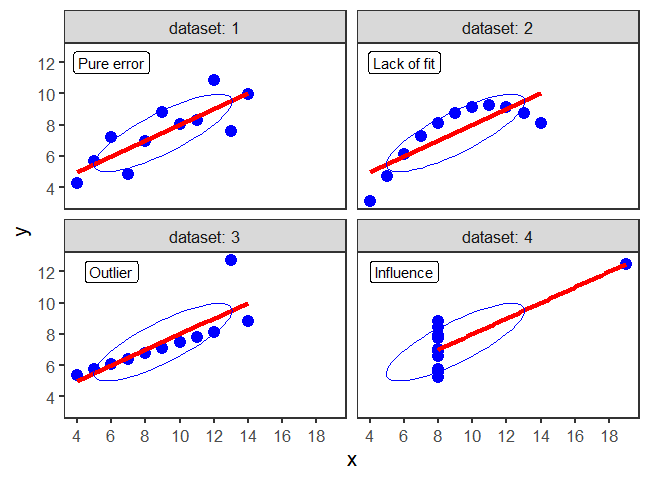
\includegraphics[width=0.9\textwidth,height=\textheight]{figs/ch02/ch02-anscombe1.png}

}

\caption{\label{fig-ch02-anscombe1}Scatterplots of Anscombe's Quartet.
Each plot shows the fitted regression line and a 68\% data ellipse
representing the correlation between \(x\) and \(y\).}

\end{figure}

This figure is produced as follows, using a single call to
\texttt{ggplot()}, faceted by \texttt{dataset}. As we will see later
(Section~\ref{sec-data-ellipse}), the data ellipse (produced by
\texttt{stat\_ellipse()}) reflects the correlation between the
variables.

\begin{Shaded}
\begin{Highlighting}[]
\NormalTok{desc }\OtherTok{\textless{}{-}} \FunctionTok{tibble}\NormalTok{(}
  \AttributeTok{dataset =} \DecValTok{1}\SpecialCharTok{:}\DecValTok{4}\NormalTok{,}
  \AttributeTok{label =} \FunctionTok{c}\NormalTok{(}\StringTok{"Pure error"}\NormalTok{, }\StringTok{"Lack of fit"}\NormalTok{, }\StringTok{"Outlier"}\NormalTok{, }\StringTok{"Influence"}\NormalTok{)}
\NormalTok{)}

\FunctionTok{ggplot}\NormalTok{(anscombe\_long, }\FunctionTok{aes}\NormalTok{(}\AttributeTok{x =}\NormalTok{ x, }\AttributeTok{y =}\NormalTok{ y)) }\SpecialCharTok{+}
  \FunctionTok{geom\_point}\NormalTok{(}\AttributeTok{color =} \StringTok{"blue"}\NormalTok{, }\AttributeTok{size =} \DecValTok{4}\NormalTok{) }\SpecialCharTok{+}
  \FunctionTok{geom\_smooth}\NormalTok{(}\AttributeTok{method =} \StringTok{"lm"}\NormalTok{, }\AttributeTok{formula =}\NormalTok{ y }\SpecialCharTok{\textasciitilde{}}\NormalTok{ x, }\AttributeTok{se =} \ConstantTok{FALSE}\NormalTok{,}
              \AttributeTok{color =} \StringTok{"red"}\NormalTok{, }\AttributeTok{linewidth =} \FloatTok{1.5}\NormalTok{) }\SpecialCharTok{+}
  \FunctionTok{scale\_x\_continuous}\NormalTok{(}\AttributeTok{breaks =} \FunctionTok{seq}\NormalTok{(}\DecValTok{0}\NormalTok{,}\DecValTok{20}\NormalTok{,}\DecValTok{2}\NormalTok{)) }\SpecialCharTok{+}
  \FunctionTok{scale\_y\_continuous}\NormalTok{(}\AttributeTok{breaks =} \FunctionTok{seq}\NormalTok{(}\DecValTok{0}\NormalTok{,}\DecValTok{12}\NormalTok{,}\DecValTok{2}\NormalTok{)) }\SpecialCharTok{+}
  \FunctionTok{stat\_ellipse}\NormalTok{(}\AttributeTok{level =} \FloatTok{0.5}\NormalTok{, }\AttributeTok{color=}\NormalTok{col, }\AttributeTok{type=}\StringTok{"norm"}\NormalTok{) }\SpecialCharTok{+}
  \FunctionTok{geom\_label}\NormalTok{(}\AttributeTok{data=}\NormalTok{desc, }\FunctionTok{aes}\NormalTok{(}\AttributeTok{label =}\NormalTok{ label), }\AttributeTok{x=}\DecValTok{6}\NormalTok{, }\AttributeTok{y=}\DecValTok{12}\NormalTok{) }\SpecialCharTok{+}
  \FunctionTok{facet\_wrap}\NormalTok{(}\SpecialCharTok{\textasciitilde{}}\NormalTok{dataset, }\AttributeTok{labeller =}\NormalTok{ label\_both) }
\end{Highlighting}
\end{Shaded}

The subplots are labeled with the statistical idea they reflect:

\begin{itemize}
\item
  dataset 1: \textbf{Pure error}. This is the typical case with
  well-behaved data. Variation of the points around the line reflect
  only measurement error or unreliability in the response, \(y\).
\item
  dataset 2: \textbf{Lack of fit}. The data is clearly curvilinear, and
  would be very well described by a quadratic,
  \texttt{y\ \textasciitilde{}\ poly(x,\ 2)}. This violates the
  assumption of linear regression that the fitted model has the correct
  form.
\item
  dataset 3: \textbf{Outlier}. One point, second from the right, has a
  very large residual. Because this point is near the extreme of \(x\),
  it pulls the regression line towards it, as you can see by imagining a
  line through the remaining points.
\item
  dataset 4: \textbf{Influence}. All but one of the points have the same
  \(x\) value. The one unusual point has sufficient influence to force
  the regression line to fit it \textbf{exactly}.
\end{itemize}

One moral from this example:

\begin{quote}
\textbf{Linear regression only ``sees'' a line. It does its' best when
the data are really linear. Because the line is fit by least squares, it
pulls the line toward discrepant points to minimize the sum of squared
residuals.}
\end{quote}

\begin{tcolorbox}[enhanced jigsaw, colback=white, rightrule=.15mm, left=2mm, arc=.35mm, colframe=quarto-callout-note-color-frame, toptitle=1mm, breakable, leftrule=.75mm, opacityback=0, bottomtitle=1mm, colbacktitle=quarto-callout-note-color!10!white, opacitybacktitle=0.6, titlerule=0mm, toprule=.15mm, title=\textcolor{quarto-callout-note-color}{\faInfo}\hspace{0.5em}{Datasaurus Dozen}, bottomrule=.15mm, coltitle=black]

The method Anscombe used to compose his quartet is unknown, but it turns
out that that there is a method to construct a wider collection of
datasets with identical statistical properties. After all, in a
bivariate dataset with \(n\) observations, the correlation has \((n-2)\)
degrees of freedom, so it is possible to choose \(n-2\) of the
\((x, y)\) pairs to yield any given value. As it happens, it is also
possible to create any number of datasets with the same means, standard
deviations and correlations with nearly any shape you like --- even a
dinosaur!

The \emph{Datasaurus Dozen} was first publicized by Alberto Cairo in a
\href{http://www.thefunctionalart.com/2016/08/download-datasaurus-never-trust-summary.html}{blog
post} and are available in the \textbf{datasauRus} package Davies et al.
(\protect\hyperlink{ref-R-datasauRus}{2022}). As shown in
\textbf{?@fig-datasaurus}, the sets include a star, cross, circle,
bullseye, horizontal and vertical lines, and, of course the ``dino''.
The method (\protect\hyperlink{ref-MatejkaFitzmaurice2017}{Matejka \&
Fitzmaurice, 2017}) uses \emph{simulated annealing}, an iterative
process that perturbs the points in a scatterplot, moving them towards a
given shape while keeping the statistical summaries close to the fixed
target value.

The \textbf{datasauRus} package just contains the datasets, but a
general method, called \emph{statistical metamers}, for producing such
datasets has been described by
\href{https://eliocamp.github.io/codigo-r/en/2019/01/statistical-metamerism/}{Elio
Campitelli} and implemented in the \textbf{metamer} package.

\end{tcolorbox}

\begin{tcolorbox}[enhanced jigsaw, colback=white, rightrule=.15mm, left=2mm, arc=.35mm, colframe=quarto-callout-note-color-frame, toptitle=1mm, breakable, leftrule=.75mm, opacityback=0, bottomtitle=1mm, colbacktitle=quarto-callout-note-color!10!white, opacitybacktitle=0.6, titlerule=0mm, toprule=.15mm, title=\textcolor{quarto-callout-note-color}{\faInfo}\hspace{0.5em}{Quartets}, bottomrule=.15mm, coltitle=black]

The essential idea of a statistical ``quartet'' is to illustrate four
quite different datasets or circumstances that seem superficially the
same, but yet are paradoxically very different when you look behind the
scenes. For example, in the context of causal analysis Gelman et al.
(\protect\hyperlink{ref-Gelman-etal:2023}{2023}), illustrated sets of
four graphs, within each of which all four represent the same average
(latent) causal effect but with much different patterns of individual
effects; McGowan et al. (\protect\hyperlink{ref-McGowan2023}{2023})
provide another illustration with four seemingly identical data sets
each generated by a different causal mechanism. As an example of machine
learning models, Biecek et al.
(\protect\hyperlink{ref-Biecek-etal:2023}{2023}), introduced the
``Rashamon Quartet'', a synthetic dataset for which four models from
different classes (linear model, regression tree, random forest, neural
network) have practically identical predictive performance. In all
cases, the paradox is solved when their visualization reveals the
distinct ways of understanding structure in the data. The
\href{https://r-causal.github.io/quartets/}{\textbf{quartets}} package
contains these and other variations on this theme.

\end{tcolorbox}

\hypertarget{sec-davis}{%
\subsection{A real example}\label{sec-davis}}

In the mid 1980s, a consulting client had a strange problem. She was
conducting a study of the relation between body image and weight
preoccupation in exercising and non-exercising people
(\protect\hyperlink{ref-Davis:1990}{Davis, 1990}). As part of the
design, the researcher wanted to know if self-reported weight could be
taken as a reliable indicator of true weight measured on a scale. It was
expected that the correlations between reported and measured weight
should be close to 1.0, and the slope of the regression lines for men
and women should also be close to 1.0. The dataset is
\texttt{car::Davis}.

She was therefore very surprise to see the following numerical results:
For men, the correlation was nearly perfect, but not so for women.

\begin{Shaded}
\begin{Highlighting}[]
\FunctionTok{data}\NormalTok{(Davis, }\AttributeTok{package=}\StringTok{"carData"}\NormalTok{)}
\NormalTok{Davis }\OtherTok{\textless{}{-}}\NormalTok{ Davis }\SpecialCharTok{|\textgreater{}}
  \FunctionTok{drop\_na}\NormalTok{()          }\CommentTok{\# drop missing cases}
\NormalTok{Davis }\SpecialCharTok{|\textgreater{}}
  \FunctionTok{group\_by}\NormalTok{(sex) }\SpecialCharTok{|\textgreater{}}
  \FunctionTok{select}\NormalTok{(sex, weight, repwt) }\SpecialCharTok{|\textgreater{}}
  \FunctionTok{summarise}\NormalTok{(}\AttributeTok{r =} \FunctionTok{cor}\NormalTok{(weight, repwt))}
\CommentTok{\#\textgreater{} \# A tibble: 2 x 2}
\CommentTok{\#\textgreater{}   sex       r}
\CommentTok{\#\textgreater{}   \textless{}fct\textgreater{} \textless{}dbl\textgreater{}}
\CommentTok{\#\textgreater{} 1 F     0.501}
\CommentTok{\#\textgreater{} 2 M     0.979}
\end{Highlighting}
\end{Shaded}

Similarly, the regression lines showed the expected slope for men, but
that for women was only 0.26.

\begin{Shaded}
\begin{Highlighting}[]
\NormalTok{Davis }\SpecialCharTok{|\textgreater{}}
  \FunctionTok{nest}\NormalTok{(}\AttributeTok{data =} \SpecialCharTok{{-}}\NormalTok{sex) }\SpecialCharTok{|\textgreater{}}
  \FunctionTok{mutate}\NormalTok{(}\AttributeTok{model =} \FunctionTok{map}\NormalTok{(data, }\SpecialCharTok{\textasciitilde{}} \FunctionTok{lm}\NormalTok{(repwt }\SpecialCharTok{\textasciitilde{}}\NormalTok{ weight, }\AttributeTok{data =}\NormalTok{ .)),}
         \AttributeTok{tidied =} \FunctionTok{map}\NormalTok{(model, tidy)) }\SpecialCharTok{|\textgreater{}}
  \FunctionTok{unnest}\NormalTok{(tidied) }\SpecialCharTok{|\textgreater{}}
  \FunctionTok{filter}\NormalTok{(term }\SpecialCharTok{==} \StringTok{"weight"}\NormalTok{) }\SpecialCharTok{|\textgreater{}}
  \FunctionTok{select}\NormalTok{(sex, term, estimate, std.error)}
\CommentTok{\#\textgreater{} \# A tibble: 2 x 4}
\CommentTok{\#\textgreater{}   sex   term   estimate std.error}
\CommentTok{\#\textgreater{}   \textless{}fct\textgreater{} \textless{}chr\textgreater{}     \textless{}dbl\textgreater{}     \textless{}dbl\textgreater{}}
\CommentTok{\#\textgreater{} 1 M     weight    0.990    0.0229}
\CommentTok{\#\textgreater{} 2 F     weight    0.262    0.0459}
\end{Highlighting}
\end{Shaded}

What could be wrong here?, the client asked. The consultant replied with
the obvious question:

\begin{quote}
\emph{Did you plot your data?}
\end{quote}

The answer turned out to be one discrepant point, a female, whose
measured weight was 166 kg (366 lbs!). This single point exerted so much
influence that it pulled the fitted regression line down to a slope of
only 0.26.

\begin{Shaded}
\begin{Highlighting}[]
\NormalTok{Davis }\SpecialCharTok{|\textgreater{}}
  \FunctionTok{ggplot}\NormalTok{(}\FunctionTok{aes}\NormalTok{(}\AttributeTok{x =}\NormalTok{ weight, }\AttributeTok{y =}\NormalTok{ repwt, }
             \AttributeTok{color =}\NormalTok{ sex, }\AttributeTok{shape=}\NormalTok{sex)) }\SpecialCharTok{+}
  \FunctionTok{geom\_point}\NormalTok{(}\AttributeTok{size =} \FunctionTok{ifelse}\NormalTok{(Davis}\SpecialCharTok{$}\NormalTok{weight}\SpecialCharTok{==}\DecValTok{166}\NormalTok{, }\DecValTok{6}\NormalTok{, }\DecValTok{2}\NormalTok{)) }\SpecialCharTok{+}
  \FunctionTok{labs}\NormalTok{(}\AttributeTok{y =} \StringTok{"Measured weight (kg)"}\NormalTok{, }
       \AttributeTok{x =} \StringTok{"Reported weight (kg)"}\NormalTok{) }\SpecialCharTok{+}
  \FunctionTok{geom\_smooth}\NormalTok{(}\AttributeTok{method =} \StringTok{"lm"}\NormalTok{, }\AttributeTok{formula =}\NormalTok{ y}\SpecialCharTok{\textasciitilde{}}\NormalTok{x, }\AttributeTok{se =} \ConstantTok{FALSE}\NormalTok{) }\SpecialCharTok{+}
  \FunctionTok{theme}\NormalTok{(}\AttributeTok{legend.position =} \FunctionTok{c}\NormalTok{(.}\DecValTok{8}\NormalTok{, .}\DecValTok{8}\NormalTok{))}
\end{Highlighting}
\end{Shaded}

\begin{figure}[H]

{\centering 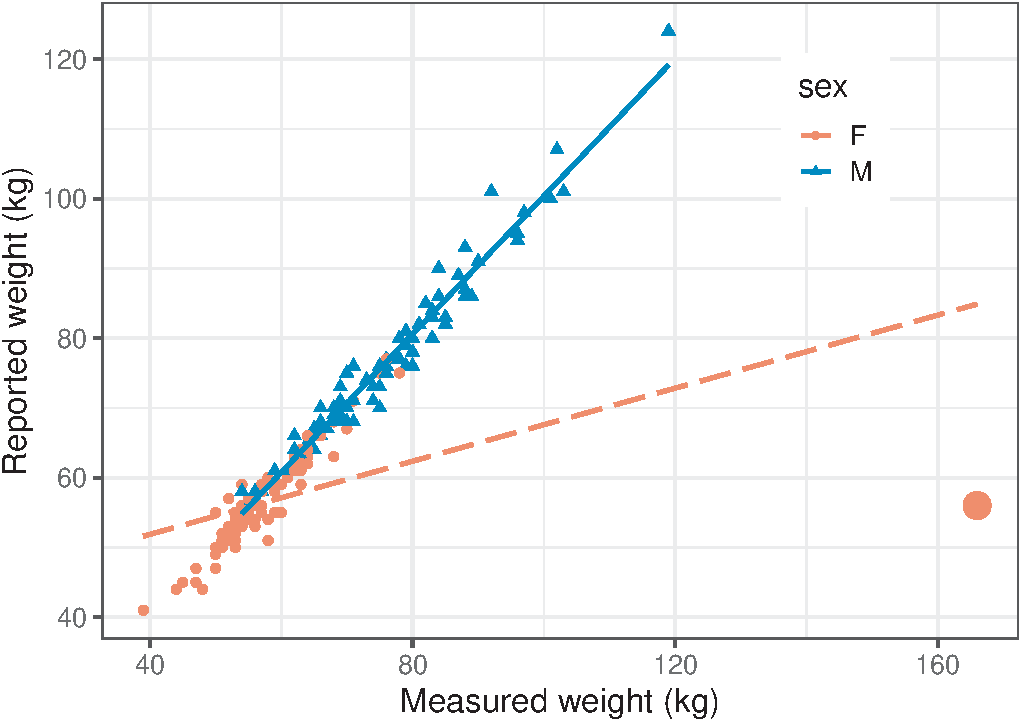
\includegraphics{figs/ch02/fig-ch02-davis-reg1-1.pdf}

}

\caption{\label{fig-ch02-davis-reg1}Regression for Davis' data on
reported weight and measures weight for men and women. Separate
regression lines, predicting reported weight from measured weight are
shown for males and females. One highly unusual point is highlighted.}

\end{figure}

In this example, it was arguable that \(x\) and \(y\) axes should be
reversed, to determine how well measured weight can be predicted from
reported weight. In \texttt{ggplot} this can easily be done by reversing
the \texttt{x} and \texttt{y} aesthetics.

\begin{Shaded}
\begin{Highlighting}[]
\NormalTok{Davis }\SpecialCharTok{|\textgreater{}}
  \FunctionTok{ggplot}\NormalTok{(}\FunctionTok{aes}\NormalTok{(}\AttributeTok{y =}\NormalTok{ weight, }\AttributeTok{x =}\NormalTok{ repwt, }\AttributeTok{color =}\NormalTok{ sex, }\AttributeTok{shape=}\NormalTok{sex)) }\SpecialCharTok{+}
  \FunctionTok{geom\_point}\NormalTok{(}\AttributeTok{size =} \FunctionTok{ifelse}\NormalTok{(Davis}\SpecialCharTok{$}\NormalTok{weight}\SpecialCharTok{==}\DecValTok{166}\NormalTok{, }\DecValTok{6}\NormalTok{, }\DecValTok{2}\NormalTok{)) }\SpecialCharTok{+}
  \FunctionTok{labs}\NormalTok{(}\AttributeTok{y =} \StringTok{"Measured weight (kg)"}\NormalTok{, }\AttributeTok{x =} \StringTok{"Reported weight (kg)"}\NormalTok{) }\SpecialCharTok{+}
  \FunctionTok{geom\_smooth}\NormalTok{(}\AttributeTok{method =} \StringTok{"lm"}\NormalTok{, }\AttributeTok{formula =}\NormalTok{ y}\SpecialCharTok{\textasciitilde{}}\NormalTok{x, }\AttributeTok{se =} \ConstantTok{FALSE}\NormalTok{) }\SpecialCharTok{+}
  \FunctionTok{theme}\NormalTok{(}\AttributeTok{legend.position =} \FunctionTok{c}\NormalTok{(.}\DecValTok{8}\NormalTok{, .}\DecValTok{8}\NormalTok{))}
\end{Highlighting}
\end{Shaded}

\begin{figure}[H]

{\centering 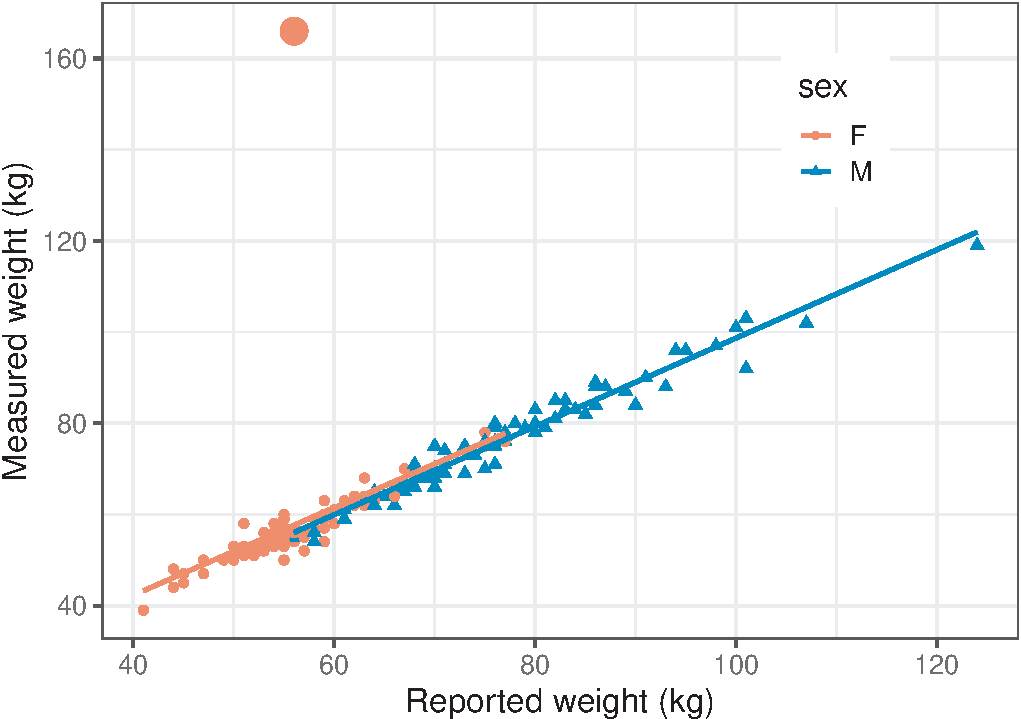
\includegraphics{figs/ch02/fig-ch02-davis-reg2-1.pdf}

}

\caption{\label{fig-ch02-davis-reg2}Regression for Davis' data on
reported weight and measures weight for men and women. Separate
regression lines, predicting measured weight from re{[}ported{]} weight
are shown for males and females. The highly unusual point no longer has
an effect on the fitted lines.}

\end{figure}

In Figure~\ref{fig-ch02-davis-reg2}, this discrepant observation again
stands out like a sore thumb, but it makes very little difference in the
fitted line for females. The reason is that this point is well within
the range of the \(x\) variable (\texttt{repwt}). To impact the slope of
the regression line, an observation must be unusual in\_both\_ \(x\) and
\(y\). We take up the topic of how to detect influential observations
and what to do about them in Chapter XX.

The value of such plots is not only that they can reveal possible
problems with an analysis, but also help identify their reasons and
suggest corrective action. What went wrong here? Examination of the
original data showed that this person switched the values, recording her
reported weight in the box for measured weight and vice versa.

\hypertarget{plots-for-data-analysis}{%
\section{Plots for data analysis}\label{plots-for-data-analysis}}

Visualization methods take an enormous variety of forms, but it is
useful to distinguish several broad categories according to their use in
data analysis:

\begin{itemize}
\item
  \textbf{data plots} : primarily plot the raw data, often with
  annotations to aid interpretation (regression lines and smooths, data
  ellipses, marginal distributions)
\item
  \textbf{reconnaissance plots} : with more than a few variables,
  reconnaissance plots provide a high-level, bird's-eye overview of the
  data, allowing you to see patterns that might not be visible in a set
  of separate plots. Some examples are scatterplot matrices, showing all
  bivariate plots of variables in a dataset; correlation diagrams, using
  visual glyphs to represent the correlations between all pairs of
  variables and ``trellis'' or faceted plots that show how a focal
  relation of one or more variables differs across values of other
  variables.
\item
  \textbf{model plots} : plot the results of a fitted model, such as a
  regression line or curve to show uncertainty, or a regression surface
  in 3D, or a plot of coefficients in model together with confidence
  intervals. Other model plots try to take into account that a fitted
  model may involve more variables than can be shown in a static 2D
  plot. Some examples of these are added variable plots, and marginal
  effect plots, both of which attempt to show the net relation of two
  focal variables, controlling or adjusting for other variables in a
  model.
\item
  \textbf{diagnostic plots} : indicating potential problems with the
  fitted model. These include residual plots, influence plots, plots for
  testing homogeneity of variance and so forth.
\item
  \textbf{dimension reduction plots} : plot representations of the data
  into a space of fewer dimensions than the number of variables in the
  dataset. Simple examples include principal components analysis (PCA)
  and the related biplots, and multidimensional scaling (MDS) methods.
\end{itemize}

We give some more details and a few examples in the sections that
follow.

\hypertarget{data-plots}{%
\section{Data plots}\label{data-plots}}

Data plots portray the data in a space where the coordinate axes are the
observed variables.

\begin{itemize}
\tightlist
\item
  1D plots include line plots, histograms and density estimates.
\item
  2D plots are most often scatterplots, but contour plots or hex-binned
  plots are also useful when the sample size is large.
\end{itemize}

\hypertarget{model-plots}{%
\section{Model plots}\label{model-plots}}

Model plots show the fitted or predicted values from a statistical model
and provide visual summaries\ldots{}

\hypertarget{diagnostic-plots}{%
\section{Diagnostic plots}\label{diagnostic-plots}}

\hypertarget{principles-of-graphical-display}{%
\section{Principles of graphical
display}\label{principles-of-graphical-display}}

{[}This could be a separate chapter{]}

\begin{itemize}
\tightlist
\item
  Criteria for assessing graphs: communication goals
\item
  Effective data display:

  \begin{itemize}
  \tightlist
  \item
    Make the data stand out
  \item
    Make graphical comparison easy
  \item
    Effect ordering: For variables and unordered factors, arrange them
    according to the effects to be seen
  \end{itemize}
\item
  Visual thinning: As the data becomes more complex, focus more on
  impactful summaries
\end{itemize}

Packages used here: 19 packages used here: base, broom, datasets, dplyr,
forcats, ggplot2, graphics, grDevices, knitr, lubridate, methods, purrr,
readr, stats, stringr, tibble, tidyr, tidyverse, utils

\bookmarksetup{startatroot}

\hypertarget{sec-multivariate_plots}{%
\chapter{Plots of Multivariate Data}\label{sec-multivariate_plots}}

\begin{quote}
There is no excuse for failing to plot and look.

The greatest value of a picture is when it forces us to notice what we
never expected to see. --- John W. Tukey, \emph{Exploratory Data
Analysis}, 1977
\end{quote}

These quotes from John Tukey remind us that data analysis should nearly
always start with graphs to help us understand the main features of our
data. It is important to understand the general \emph{patterns} and
\emph{trends}: Are relationships increasing or decreasing? Are they
approximately linear or non-linear? But it is also important to spot
\emph{anomalies}: ``unusual'' observations, groups of points that seem
to differ from the rest, and so forth. As we saw with Anscombe's quartet
(Section~\ref{sec-anscombe}) numerical summaries hide features that are
immediately apparent in a plot.

This chapter introduces a toolbox of basic graphical methods for
visualizing multivariate datasets. It starts with some simple techniques
to enhance the basic scatterplot with graphical \emph{annotations} such
as fitted lines, curves and data ellipses to \emph{summarize} the
relation between two variables.

To visualize more than two variables, we can view all pairs of variables
in a scatterplot matrix or shift gears entirely to show multiple
variables along a set of parallel axes. As the number of variables
increases, we may need to suppress details with stronger summaries for a
high-level reconnaissance of our data terrain, as we do by zooming out
on a map. For example, we can simply remove the data points or make them
nearly transparent to focus on the visual summaries provided by fitted
lines or other graphical summaries.

\textbf{Packages}

In this chapter I use the following packages. Load them now:

\begin{Shaded}
\begin{Highlighting}[]
\FunctionTok{library}\NormalTok{(car)}
\FunctionTok{library}\NormalTok{(ggplot2)}
\FunctionTok{library}\NormalTok{(dplyr)}
\FunctionTok{library}\NormalTok{(tidyr)}
\FunctionTok{library}\NormalTok{(corrplot)}
\FunctionTok{library}\NormalTok{(corrgram)}
\FunctionTok{library}\NormalTok{(GGally)}
\FunctionTok{library}\NormalTok{(ggdensity)}
\FunctionTok{library}\NormalTok{(patchwork)}
\FunctionTok{library}\NormalTok{(ggpcp)}
\end{Highlighting}
\end{Shaded}

\hypertarget{sec-bivariate_summaries}{%
\section{Bivariate summaries}\label{sec-bivariate_summaries}}

The basic scatterplot is the workhorse of multivariate data
visualization, showing how one variable, \(y\), often an outcome to be
explained by or varies with another, \(x\). It is a building block for
many useful techniques, so it is helpful to understand how it can be
used as a tool for thinking in a wider, multivariate context.

The essential idea is that we can start with a simple version of the
scatterplot and add annotations to show interesting features more
clearly. We consider the following here:

\begin{itemize}
\tightlist
\item
  \textbf{Smoothers}: Showing overall trends, perhaps in several forms,
  as visual summaries such as fitted regression lines or curves and
  nonparametric smoothers.
\item
  \textbf{Stratifiers}: Using color, shape or other features to identify
  subgroups; more generally, \emph{conditioning} on other variables in
  multi-panel displays;
\item
  \textbf{Data ellipses}: A compact 2D visual summary of bivariate
  linear relations and uncertainty assuming normality; more generally,
  contour plots of bivariate density.
\end{itemize}

\textbf{Example: Academic salaries}

Let's start with data on the academic salaries of faculty members
collected at a U.S. college for the purpose of assessing salary
differences between male and female faculty members, and perhaps address
anomalies in compensation. The dataset \texttt{carData::Salaries} gives
data on nine-month salaries and other variables for 397 faculty members
in the 2008-2009 academic year.

\begin{Shaded}
\begin{Highlighting}[]
\FunctionTok{data}\NormalTok{(Salaries, }\AttributeTok{package =} \StringTok{"carData"}\NormalTok{)}
\FunctionTok{str}\NormalTok{(Salaries)}
\CommentTok{\#\textgreater{} \textquotesingle{}data.frame\textquotesingle{}:    397 obs. of  6 variables:}
\CommentTok{\#\textgreater{}  $ rank         : Factor w/ 3 levels "AsstProf","AssocProf",..: 3 3 1 3 3 2 3 3 3 3 ...}
\CommentTok{\#\textgreater{}  $ discipline   : Factor w/ 2 levels "A","B": 2 2 2 2 2 2 2 2 2 2 ...}
\CommentTok{\#\textgreater{}  $ yrs.since.phd: int  19 20 4 45 40 6 30 45 21 18 ...}
\CommentTok{\#\textgreater{}  $ yrs.service  : int  18 16 3 39 41 6 23 45 20 18 ...}
\CommentTok{\#\textgreater{}  $ sex          : Factor w/ 2 levels "Female","Male": 2 2 2 2 2 2 2 2 2 1 ...}
\CommentTok{\#\textgreater{}  $ salary       : int  139750 173200 79750 115000 141500 97000 175000 147765 119250 129000 ...}
\end{Highlighting}
\end{Shaded}

The most obvious, but perhaps naive, predictor of \texttt{salary} is
\texttt{years.since.phd}. For simplicity, I'll refer to this as years of
``experience.'' Before looking at differences between males and females,
we would want consider faculty \texttt{rank} (related also to
\texttt{yrs.service}) and \texttt{discipline}, recorded here as
\texttt{A} (``theoretical'' departments) or \texttt{B} (``applied''
departments). But, for a basic plot, we will ignore these for now to
focus on what can be learned from plot annotations.

\begin{Shaded}
\begin{Highlighting}[]
\FunctionTok{library}\NormalTok{(ggplot2)}
\NormalTok{gg1 }\OtherTok{\textless{}{-}} \FunctionTok{ggplot}\NormalTok{(Salaries, }
       \FunctionTok{aes}\NormalTok{(}\AttributeTok{x =}\NormalTok{ yrs.since.phd, }\AttributeTok{y =}\NormalTok{ salary)) }\SpecialCharTok{+}
  \FunctionTok{geom\_jitter}\NormalTok{(}\AttributeTok{size =} \DecValTok{2}\NormalTok{) }\SpecialCharTok{+}
  \FunctionTok{scale\_y\_continuous}\NormalTok{(}\AttributeTok{labels =}\NormalTok{ scales}\SpecialCharTok{::}\FunctionTok{dollar\_format}\NormalTok{(}
    \AttributeTok{prefix=}\StringTok{"$"}\NormalTok{, }\AttributeTok{scale =} \FloatTok{0.001}\NormalTok{, }\AttributeTok{suffix =} \StringTok{"K"}\NormalTok{)) }\SpecialCharTok{+}
  \FunctionTok{labs}\NormalTok{(}\AttributeTok{x =} \StringTok{"Years since PhD"}\NormalTok{,}
       \AttributeTok{y =} \StringTok{"Salary"}\NormalTok{) }

\NormalTok{gg1}
\end{Highlighting}
\end{Shaded}

\begin{figure}[H]

{\centering 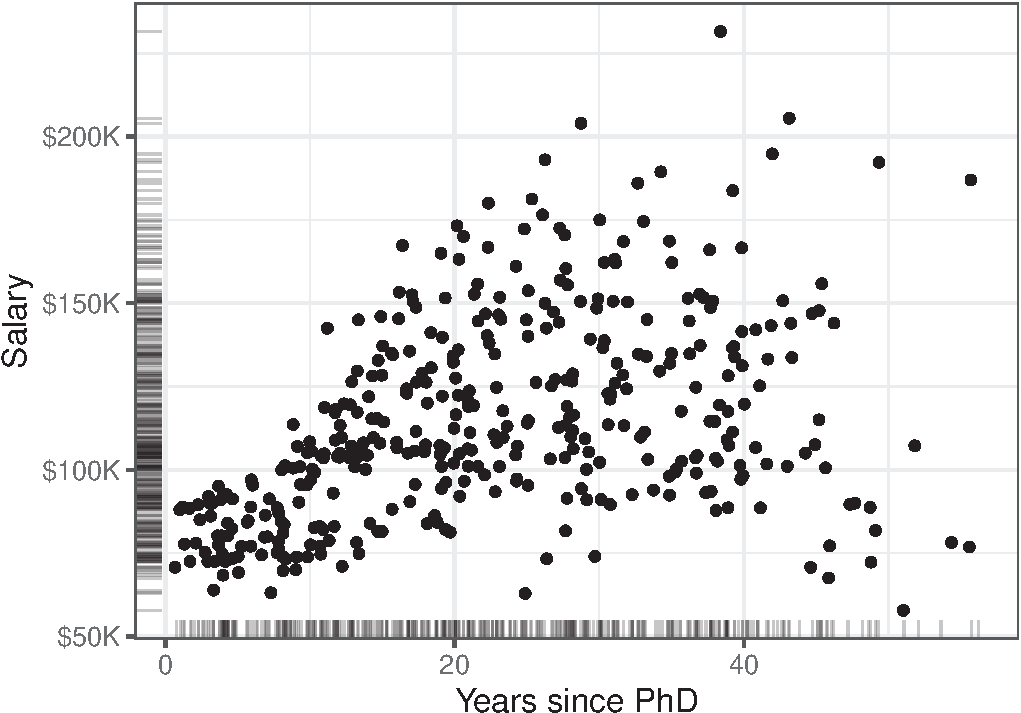
\includegraphics[width=0.8\textwidth,height=\textheight]{figs/ch03/fig-Salaries-scat-1.pdf}

}

\caption{\label{fig-Salaries-scat}Naive scatterplot of Salary vs.~years
since PhD, ignoring other variables, and without graphical annotations.}

\end{figure}

There is quite a lot we can see ``just by looking'' at this simple plot,
but the main things are:

\begin{itemize}
\tightlist
\item
  Salary increases generally from 0 - 40 years since the PhD;
\item
  Variability in salary increases among those with the same experience,
  a ``fan-shaped'' pattern that signals a violation of homogeneity of
  variance in simple regression;
\item
  Data beyond 50 years is thin, but there are some quite low salaries
  there.
\end{itemize}

\hypertarget{smoothers}{%
\subsection{Smoothers}\label{smoothers}}

Smoothers are among the most useful graphical annotations you can add to
such plots, giving a visual summary of how \(y\) changes with \(x\). The
most common smoother is a line showing the linear regression for \(y\)
given \(x\), expressed in math notation as
\(\mathbb{E} (y | x) = b_0 + b_1 x\). If there is doubt that a linear
relation is an adequate summary, you can try a quadratic or other
polynomial smoothers.

In \textbf{ggplot2}, these are easily added to a plot using
\texttt{geom\_smooth()} with \texttt{method\ =\ "lm"}, and a model
\texttt{formula}, which (by default) is \texttt{y\ \textasciitilde{}\ x}
for a linear relation or \texttt{y\ \textasciitilde{}\ poly(x,\ k)} for
a polynomial of degree \(k\).

\begin{Shaded}
\begin{Highlighting}[]
\NormalTok{gg1 }\SpecialCharTok{+} 
  \FunctionTok{geom\_smooth}\NormalTok{(}\AttributeTok{method =} \StringTok{"lm"}\NormalTok{, }\AttributeTok{formula =} \StringTok{"y \textasciitilde{} x"}\NormalTok{, }
              \AttributeTok{color =} \StringTok{"red"}\NormalTok{, }\AttributeTok{fill=} \StringTok{"red"}\NormalTok{,}
              \AttributeTok{linewidth =} \DecValTok{2}\NormalTok{) }\SpecialCharTok{+}
  \FunctionTok{geom\_smooth}\NormalTok{(}\AttributeTok{method =} \StringTok{"lm"}\NormalTok{, }\AttributeTok{formula =} \StringTok{"y \textasciitilde{} poly(x,2)"}\NormalTok{, }
              \AttributeTok{color =} \StringTok{"darkgreen"}\NormalTok{, }\AttributeTok{fill =} \StringTok{"darkgreen"}\NormalTok{,}
              \AttributeTok{linewidth =} \DecValTok{2}\NormalTok{) }
\end{Highlighting}
\end{Shaded}

\begin{figure}[H]

{\centering 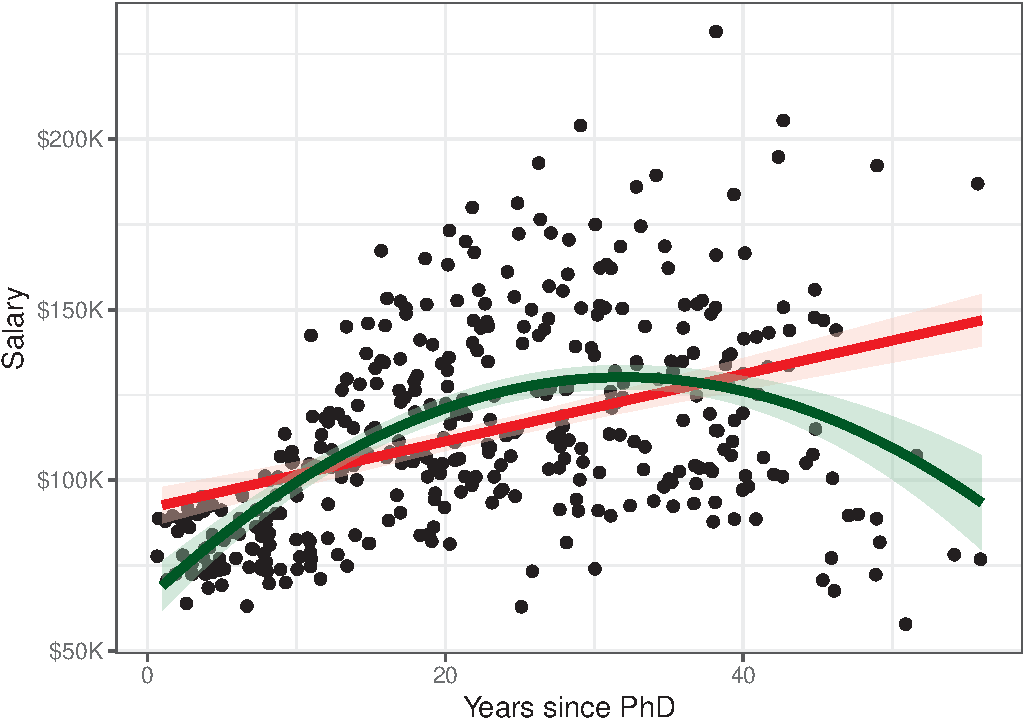
\includegraphics[width=0.8\textwidth,height=\textheight]{figs/ch03/fig-Salaries-lm-1.pdf}

}

\caption{\label{fig-Salaries-lm}Scatterplot of Salary vs.~years since
PhD, showing linear and quadratic smooths with 95\% confidence bands.}

\end{figure}

This serves to highlight some of our impressions from the basic
scatterplot shown in Figure~\ref{fig-Salaries-scat}, making them more
apparent. And that's precisely the point: the regression smoother draws
attention to a possible pattern that we can consider as a visual summary
of the data. You can think of this as showing what a linear (or
quadratic) regression ``sees'' in the data. Statistical tests can help
you decide if there is more evidence for a quadratic fit compared to the
simpler linear relation.

It is useful to also show some indication of \emph{uncertainty} (or
inversely, \emph{precision}) associated with the predicted values. Both
the linear and quadratic trends are shown in
Figure~\ref{fig-Salaries-lm} with 95\% pointwise confidence bands. These
are necessarily narrower in the center of the range of \(x\) where there
is typically more data; they get wider toward the highest values of
experience where the data are thinner.

\hypertarget{non-parametric-smoothers}{%
\subsubsection{Non-parametric
smoothers}\label{non-parametric-smoothers}}

The most generally useful idea is a smoother that tracks an average
value, \(\mathbb{E} (y | x)\), of \(y\) as \(x\) varies across its'
range \emph{without} assuming any particular functional form, and so
avoiding the necessity to choose among
\texttt{y\ \textasciitilde{}\ poly(x,\ 1)}, or
\texttt{y\ \textasciitilde{}\ poly(x,\ 2)}, or
\texttt{y\ \textasciitilde{}\ poly(x,\ 3)}, etc.

Non-parametric smoothers attempt to estimate
\(\mathbb{E} (y | x) = f(x)\) where \(f(x)\) is some smooth function.
These typically use a collection of weighted \emph{local regressions}
for each \(x_i\) within a window centered at that value. In the method
called \emph{lowess} or \emph{loess}
(\protect\hyperlink{ref-Cleveland:79}{Cleveland, 1979};
\protect\hyperlink{ref-ClevelandDevlin:88}{Cleveland \& Devlin, 1988}),
a weight function is applied, giving greatest weight to \(x_i\) and a
weight of 0 outside a window containing a certain fraction, \(s\),
called \emph{span}, of the nearest neighbors of \(x_i\). The fraction,
\(s\), is usually within the range \(1/3 \le s \le 2/3\), and it
determines the smoothness of the resulting curve; smaller values produce
a wigglier curve and larger values giving a smoother fit (an optimal
span can be determined by \(k\)-fold cross-validation to minimize a
measure of overall error of approximation).

Non-parametric regression is a broad topic; see Fox
(\protect\hyperlink{ref-Fox:2016:ARA}{2016}), Ch. 18 for a more general
treatment and Wood (\protect\hyperlink{ref-Wood:2006}{2006}) for
generalized additive models, fit using \texttt{method\ =\ "gam"} in
\textbf{ggplot2}, which is the default when the largest group has more
than 1,000 observations.

Figure~\ref{fig-Salaries-loess} shows the addition of a loess smooth to
the plot in Figure~\ref{fig-Salaries-lm}, suppressing the confidence
band for the linear regression. The loess fit is nearly coincident with
the quadratic fit, but has a slightly wider confidence band.

\begin{Shaded}
\begin{Highlighting}[]
\NormalTok{gg1 }\SpecialCharTok{+} 
  \FunctionTok{geom\_smooth}\NormalTok{(}\AttributeTok{method =} \StringTok{"loess"}\NormalTok{, }\AttributeTok{formula =} \StringTok{"y \textasciitilde{} x"}\NormalTok{, }
              \AttributeTok{color =} \StringTok{"blue"}\NormalTok{, }\AttributeTok{fill =}\NormalTok{ scales}\SpecialCharTok{::}\FunctionTok{muted}\NormalTok{(}\StringTok{"blue"}\NormalTok{),}
              \AttributeTok{linewidth =} \DecValTok{2}\NormalTok{) }\SpecialCharTok{+}
  \FunctionTok{geom\_smooth}\NormalTok{(}\AttributeTok{method =} \StringTok{"lm"}\NormalTok{, }\AttributeTok{formula =} \StringTok{"y \textasciitilde{} x"}\NormalTok{, }\AttributeTok{se =} \ConstantTok{FALSE}\NormalTok{,}
              \AttributeTok{color =} \StringTok{"red"}\NormalTok{,}
              \AttributeTok{linewidth =} \DecValTok{2}\NormalTok{) }\SpecialCharTok{+}
  \FunctionTok{geom\_smooth}\NormalTok{(}\AttributeTok{method =} \StringTok{"lm"}\NormalTok{, }\AttributeTok{formula =} \StringTok{"y \textasciitilde{} poly(x,2)"}\NormalTok{, }
              \AttributeTok{color =} \StringTok{"darkgreen"}\NormalTok{, }\AttributeTok{fill =} \StringTok{"lightgreen"}\NormalTok{,}
              \AttributeTok{linewidth =} \DecValTok{2}\NormalTok{) }
\end{Highlighting}
\end{Shaded}

\begin{figure}[H]

{\centering 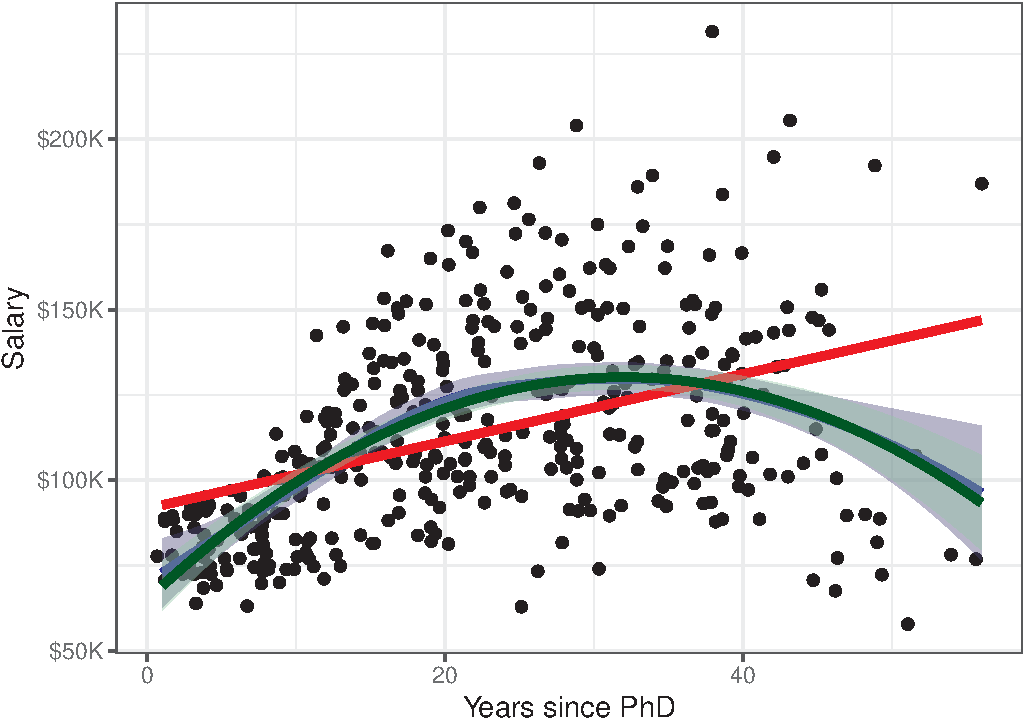
\includegraphics[width=0.8\textwidth,height=\textheight]{figs/ch03/fig-Salaries-loess-1.pdf}

}

\caption{\label{fig-Salaries-loess}Scatterplot of Salary vs.~years since
PhD, adding the loess smooth.}

\end{figure}

But now comes an important question: is it reasonable that academic
salary should increase up to about 40 years since the PhD degree and
then decline? The predicted salary for someone still working 50 years
after earning their degree is about the same as a person at 15 years.
What else is going on here?

\hypertarget{stratifiers}{%
\subsection{Stratifiers}\label{stratifiers}}

Very often, we have a main relationship of interest, but various groups
in the data are identified by discrete factors (like faculty
\texttt{rank} and \texttt{sex}, their type of \texttt{discipline} here),
or there are quantitative predictors for which the main relation might
vary. In the language of statistical models such effects are
\emph{interaction} terms, as in
\texttt{y\ \textasciitilde{}\ group\ +\ x\ +\ group:x}, where the term
\texttt{group:x} fits a different slope for each group and the grouping
variable is often called a \emph{moderator} variable. Common moderator
variables are ethnicity, health status, social class and level of
education. Moderators can also be continuous variables as in
\texttt{y\ \textasciitilde{}\ x1\ +\ x2\ +\ x1:x2}.

I call these \emph{stratifiers}, recognizing that we should consider
breaking down the overall relation to see whether and how it changes
over such ``other'' variables. Such variables are most often factors,
but we can cut a continuous variable into ranges (\emph{shingles}) and
do the same graphically. There are two general stratifying graphical
techniques:

\begin{itemize}
\item
  \textbf{Grouping}: Identify subgroups in the data by assigning
  different visual attributes, such as color, shape, line style, etc.
  within a single plot. This is quite natural for factors; quantitative
  predictors can be accommodated by cutting their range into ordered
  intervals. Grouping has the advantage that the levels of a grouping
  variable can be shown within the same plot, facilitating direct
  comparison.
\item
  \textbf{Conditioning}: Showing subgroups in different plot panels.
  This has the advantages that relations for the individual groups more
  easily discerned and one can easily stratify by two (or more) other
  variables jointly, but visual comparison is more difficult because the
  eye must scan from one panel to another.
\end{itemize}

\begin{tcolorbox}[enhanced jigsaw, colback=white, rightrule=.15mm, left=2mm, arc=.35mm, colframe=quarto-callout-note-color-frame, toptitle=1mm, breakable, leftrule=.75mm, opacityback=0, bottomtitle=1mm, colbacktitle=quarto-callout-note-color!10!white, opacitybacktitle=0.6, titlerule=0mm, toprule=.15mm, title=\textcolor{quarto-callout-note-color}{\faInfo}\hspace{0.5em}{History Corner}, bottomrule=.15mm, coltitle=black]

Recognition of the roles of visual grouping by factors within a panel
and conditioning in multi-panel displays was an important advance in the
development of modern statistical graphics. It began at A.T.\&T. Bell
Labs in Murray Hill, NJ in conjunction with the \textbf{S} language, the
mother of R.

Conditioning displays (originally called \emph{coplots}
(\protect\hyperlink{ref-ChambersHastie1991}{Chambers \& Hastie, 1991}))
are simply a collection of 1D, 2D or 3D plots separate panels for
subsets of the data broken down by one or more factors, or, for
quantitative variables, subdivided into a factor with several
overlapping intervals (\emph{shingles}). The first implementation was in
\emph{Trellis} plots Becker et al.
(\protect\hyperlink{ref-Becker:1996:VDC}{1996});Cleveland
(\protect\hyperlink{ref-Cleveland:85}{1985}).

Trellis displays were extended in the \textbf{lattice} package
(\protect\hyperlink{ref-R-lattice}{Sarkar, 2023}), which offered:

\begin{itemize}
\tightlist
\item
  A \textbf{graphing syntax} similar to that used in statistical model
  formulas: \texttt{y\ \textasciitilde{}\ x\ \textbar{}\ g} conditions
  the data by the levels of \texttt{g}, with \texttt{\textbar{}} read as
  ``given''; two or more conditioning are specified as
  \texttt{y\ \textasciitilde{}\ x\ \textbar{}\ g1\ +\ g2\ +\ ...}, with
  \texttt{+} read as ``and''.
\item
  \textbf{Panel functions} define what is plotted in a given panel.
  \texttt{panel.xyplot()} is the default for scatterplots, plotting
  points, but you can add \texttt{panel.lmline()} for regression lines,
  \texttt{latticeExtra::panel.smoother()} for loess smooths and a wide
  variety of others.
\end{itemize}

The \textbf{car} package (\protect\hyperlink{ref-R-car}{Fox et al.,
2023}) supports this graphing syntax in many of its functions.
\textbf{ggplot2} does not; it uses aesthetics (\texttt{aes()}), which
map variables in the data to visual characteristics in displays.

\end{tcolorbox}

The most obvious variable that affects academic salary is \texttt{rank},
because faculty typically get an increase in salary with a promotion
that carries through in their future salary. What can we see if we group
by \texttt{rank} and fit a separate smoothed curve for each?

In \texttt{ggplot2} thinking, grouping is accomplished simply by adding
an aesthetic, such as \texttt{color\ =\ rank}. What happens then is that
points, lines, smooths and other \texttt{geom\_*()} inherit the feature
that they are differentiated by color. In the case of
\texttt{geom\_smooth()}, we get a separate fit for each subset of the
data, according to \texttt{rank}.

\begin{Shaded}
\begin{Highlighting}[]
\CommentTok{\# make some re{-}useable pieces to avoid repetitions}
\NormalTok{scale\_salary }\OtherTok{\textless{}{-}}   \FunctionTok{scale\_y\_continuous}\NormalTok{(}
  \AttributeTok{labels =}\NormalTok{ scales}\SpecialCharTok{::}\FunctionTok{dollar\_format}\NormalTok{(}\AttributeTok{prefix=}\StringTok{"$"}\NormalTok{, }
                                 \AttributeTok{scale =} \FloatTok{0.001}\NormalTok{, }
                                 \AttributeTok{suffix =} \StringTok{"K"}\NormalTok{)) }
\CommentTok{\# position the legend inside the plot}
\NormalTok{legend\_pos }\OtherTok{\textless{}{-}} \FunctionTok{theme}\NormalTok{(}\AttributeTok{legend.position =} \FunctionTok{c}\NormalTok{(.}\DecValTok{1}\NormalTok{, }\FloatTok{0.95}\NormalTok{), }
                    \AttributeTok{legend.justification =} \FunctionTok{c}\NormalTok{(}\DecValTok{0}\NormalTok{, }\DecValTok{1}\NormalTok{))}

\FunctionTok{ggplot}\NormalTok{(Salaries, }
       \FunctionTok{aes}\NormalTok{(}\AttributeTok{x =}\NormalTok{ yrs.since.phd, }\AttributeTok{y =}\NormalTok{ salary, }
           \AttributeTok{color =}\NormalTok{ rank)) }\SpecialCharTok{+}
  \FunctionTok{geom\_point}\NormalTok{() }\SpecialCharTok{+}
\NormalTok{  scale\_salary }\SpecialCharTok{+}
  \FunctionTok{labs}\NormalTok{(}\AttributeTok{x =} \StringTok{"Years since PhD"}\NormalTok{,}
       \AttributeTok{y =} \StringTok{"Salary"}\NormalTok{) }\SpecialCharTok{+}
  \FunctionTok{geom\_smooth}\NormalTok{(}\FunctionTok{aes}\NormalTok{(}\AttributeTok{fill =}\NormalTok{ rank),}
                  \AttributeTok{method =} \StringTok{"loess"}\NormalTok{, }\AttributeTok{formula =} \StringTok{"y \textasciitilde{} x"}\NormalTok{, }
                  \AttributeTok{linewidth =} \DecValTok{2}\NormalTok{)  }\SpecialCharTok{+}
\NormalTok{  legend\_pos}
\end{Highlighting}
\end{Shaded}

\begin{figure}[H]

{\centering 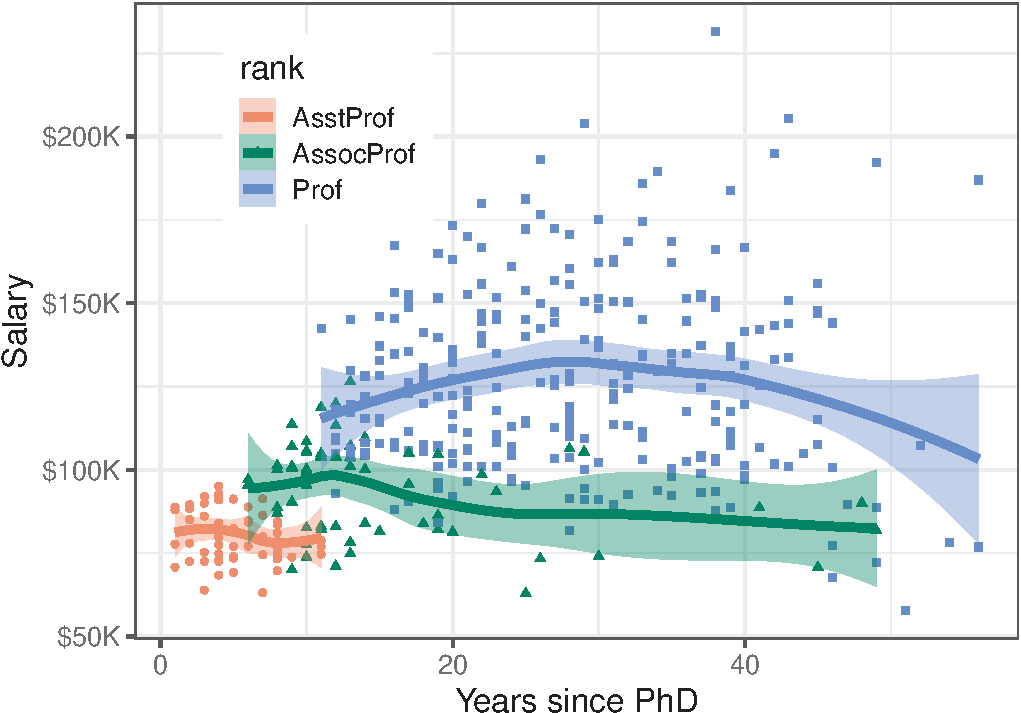
\includegraphics[width=0.8\textwidth,height=\textheight]{figs/ch03/fig-Salaries-rank-1.pdf}

}

\caption{\label{fig-Salaries-rank}Scatterplot of Salary vs.~years since
PhD, grouped by rank.}

\end{figure}

Well, there is a different story here. Salaries generally occupy
separate levels, increasing with academic rank. The horizontal extents
of the smoothed curves show their ranges. Within each rank there is some
initial increase after promotion, and then some tendency to decline with
increasing years. But, by and large, years since the PhD doesn't make
that much difference once we've taken academic rank into account.

What about the \texttt{discipline} which is classified, perhaps
peculiarly, as ``theoretical'' vs.~``applied''? The values are just
\texttt{"A"} and \texttt{"B"}, so I map these to more meaningful labels
before making the plot.

\begin{Shaded}
\begin{Highlighting}[]
\NormalTok{Salaries }\OtherTok{\textless{}{-}}\NormalTok{ Salaries }\SpecialCharTok{|\textgreater{}}
  \FunctionTok{mutate}\NormalTok{(}\AttributeTok{discipline =} \FunctionTok{factor}\NormalTok{(discipline, }
                             \AttributeTok{labels =} \FunctionTok{c}\NormalTok{(}\StringTok{"A: Theoretical"}\NormalTok{, }\StringTok{"B: Applied"}\NormalTok{)))}

\NormalTok{Salaries }\SpecialCharTok{|\textgreater{}}
  \FunctionTok{ggplot}\NormalTok{(}\FunctionTok{aes}\NormalTok{(}\AttributeTok{x =}\NormalTok{ yrs.since.phd, }\AttributeTok{y =}\NormalTok{ salary, }\AttributeTok{color =}\NormalTok{ discipline)) }\SpecialCharTok{+}
    \FunctionTok{geom\_point}\NormalTok{() }\SpecialCharTok{+}
\NormalTok{  scale\_salary }\SpecialCharTok{+}
  \FunctionTok{geom\_smooth}\NormalTok{(}\FunctionTok{aes}\NormalTok{(}\AttributeTok{fill =}\NormalTok{ discipline ),}
                \AttributeTok{method =} \StringTok{"loess"}\NormalTok{, }\AttributeTok{formula =} \StringTok{"y \textasciitilde{} x"}\NormalTok{, }
                \AttributeTok{linewidth =} \DecValTok{2}\NormalTok{) }\SpecialCharTok{+} 
  \FunctionTok{labs}\NormalTok{(}\AttributeTok{x =} \StringTok{"Years since PhD"}\NormalTok{,}
       \AttributeTok{y =} \StringTok{"Salary"}\NormalTok{) }\SpecialCharTok{+}
\NormalTok{  legend\_pos }
\end{Highlighting}
\end{Shaded}

\begin{figure}[H]

{\centering 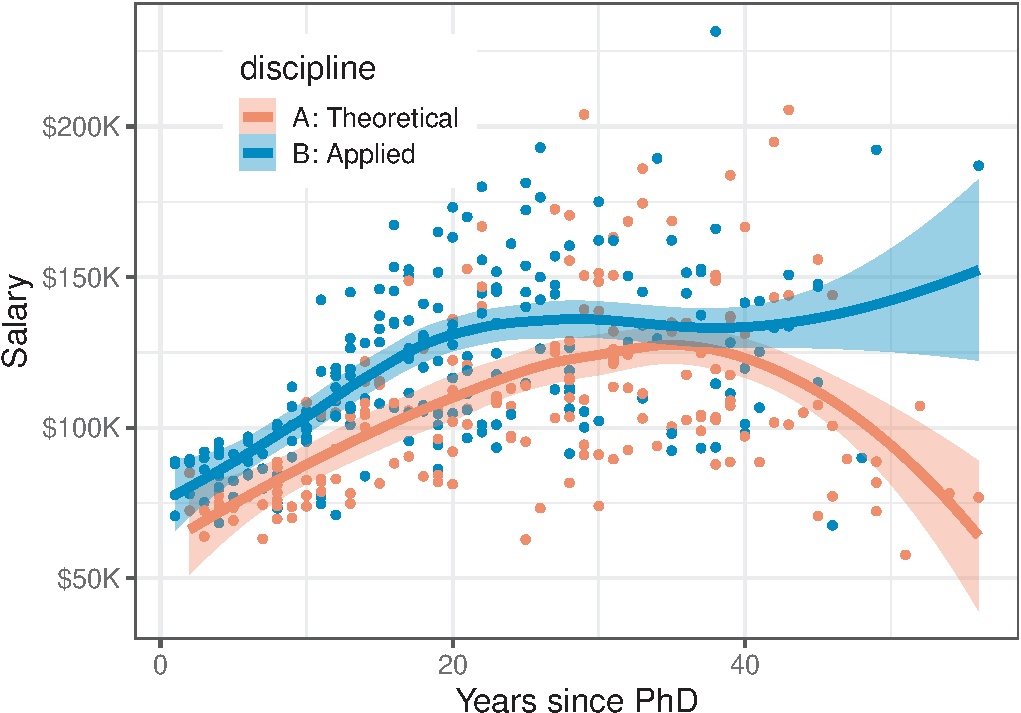
\includegraphics[width=0.8\textwidth,height=\textheight]{figs/ch03/fig-Salaries-discipline-1.pdf}

}

\caption{\label{fig-Salaries-discipline}Scatterplot of Salary vs.~years
since PhD, grouped by discipline.}

\end{figure}

The story in Figure~\ref{fig-Salaries-discipline} is again different.
Faculty in applied disciplines on average earn about 10,000\$ more per
year on average than their theoretical colleagues.

\begin{Shaded}
\begin{Highlighting}[]
\NormalTok{Salaries }\SpecialCharTok{|\textgreater{}}
  \FunctionTok{group\_by}\NormalTok{(discipline) }\SpecialCharTok{|\textgreater{}}
  \FunctionTok{summarize}\NormalTok{(}\AttributeTok{mean =} \FunctionTok{mean}\NormalTok{(salary)) }
\CommentTok{\#\textgreater{} \# A tibble: 2 x 2}
\CommentTok{\#\textgreater{}   discipline        mean}
\CommentTok{\#\textgreater{}   \textless{}fct\textgreater{}            \textless{}dbl\textgreater{}}
\CommentTok{\#\textgreater{} 1 A: Theoretical 108548.}
\CommentTok{\#\textgreater{} 2 B: Applied     118029.}
\end{Highlighting}
\end{Shaded}

For both groups, there is an approximately linear relation up to about
30--40 years, but the smoothed curves then diverge into the region where
the data is thinner.

\hypertarget{conditioning}{%
\subsection{Conditioning}\label{conditioning}}

The previous plots use grouping by color to plot the data for different
subsets inside the same plot window, making comparison among groups
easier, because they can be directly compared along a common vertical
scale \footnote{The classic study by Cleveland \& McGill
  (\protect\hyperlink{ref-ClevelandMcGill:84b}{1984});Cleveland \&
  McGill (\protect\hyperlink{ref-ClevelandMcGill:85}{1985}) shows that
  judgements of magnitude along a common scale are more accurate than
  those along separate, aligned scales.}. This gets messy, however, when
there are more than just a few levels, or worse---when there are two (or
more) variables for which we want to show separate effects. In such
cases, we can plot separate panels using the \texttt{ggplot2} concept of
\emph{faceting}. There are two options: \texttt{facet\_wrap()} takes one
or more conditioning variables and produces a ribbon of plots for each
combination of levels; \texttt{facet\_grid(row\ \textasciitilde{}\ col)}
takes two or more conditioning variables and arranges the plots in a 2D
array identified by the \texttt{row} and \texttt{col} variables.

Let's look at salary broken down by the combinations of discipline and
rank. Here, I chose to stratify using color by rank within each of
panels faceting by discipline. Because there is more going on in this
plot, a linear smooth is used to represent the trend.

\begin{Shaded}
\begin{Highlighting}[]
\NormalTok{Salaries }\SpecialCharTok{|\textgreater{}}
  \FunctionTok{ggplot}\NormalTok{(}\FunctionTok{aes}\NormalTok{(}\AttributeTok{x =}\NormalTok{ yrs.since.phd, }\AttributeTok{y =}\NormalTok{ salary, }\AttributeTok{color =}\NormalTok{ rank)) }\SpecialCharTok{+}
  \FunctionTok{geom\_point}\NormalTok{() }\SpecialCharTok{+}
\NormalTok{  scale\_salary }\SpecialCharTok{+}
  \FunctionTok{labs}\NormalTok{(}\AttributeTok{x =} \StringTok{"Years since PhD"}\NormalTok{,}
       \AttributeTok{y =} \StringTok{"Salary"}\NormalTok{) }\SpecialCharTok{+}
  \FunctionTok{geom\_smooth}\NormalTok{(}\FunctionTok{aes}\NormalTok{(}\AttributeTok{fill =}\NormalTok{ rank),}
              \AttributeTok{method =} \StringTok{"lm"}\NormalTok{, }\AttributeTok{formula =} \StringTok{"y \textasciitilde{} x"}\NormalTok{, }
              \AttributeTok{linewidth =} \DecValTok{2}\NormalTok{) }\SpecialCharTok{+}
  \FunctionTok{facet\_wrap}\NormalTok{(}\SpecialCharTok{\textasciitilde{}}\NormalTok{ discipline) }\SpecialCharTok{+}
\NormalTok{  legend\_pos}
\end{Highlighting}
\end{Shaded}

\begin{figure}[H]

{\centering 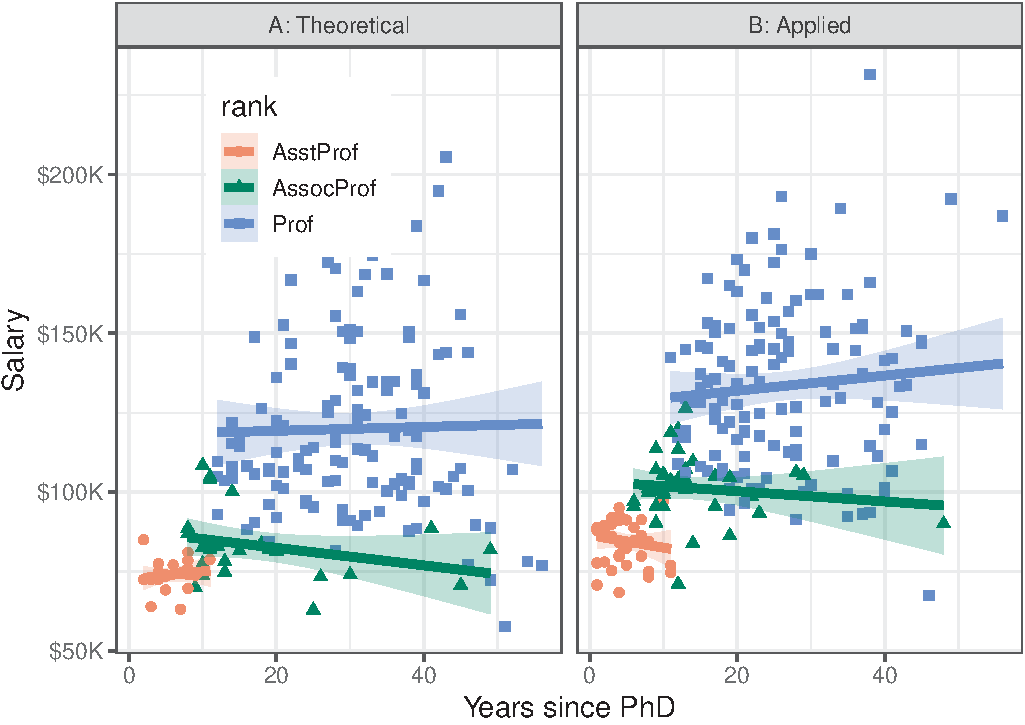
\includegraphics[width=1\textwidth,height=\textheight]{figs/ch03/fig-Salaries-faceted-1.pdf}

}

\caption{\label{fig-Salaries-faceted}Scatterplot of Salary vs.~years
since PhD, grouped by rank, with separate panels for discipline.}

\end{figure}

Once both of these factors are taken into account, there does not seem
to be much impact of years of service. Salaries in theoretical
disciplines are noticeably greater than those in applied disciplines at
all ranks, and there are even greater differences among ranks.

Finally, to shed light on the question that motivated this example---
are there anomalous differences in salary for men and women--- we can
look at differences in salary according to sex, when discipline and rank
are taken into account. To do this graphically, condition by both
variables, but use
\texttt{facet\_grid(discipline\ \textasciitilde{}\ rank)} to arrange
their combinations in a grid whose rows are the levels of
\texttt{discipline} and columns are those of \texttt{rank}. I want to
make the comparison of males and females most direct, so I use
\texttt{color\ =\ sex} to stratify the panels. The smoothed regression
lines and error bands are calculated separately for each combination of
discipline, rank and sex.

\begin{Shaded}
\begin{Highlighting}[]
\NormalTok{Salaries }\SpecialCharTok{|\textgreater{}}
  \FunctionTok{ggplot}\NormalTok{(}\FunctionTok{aes}\NormalTok{(}\AttributeTok{x =}\NormalTok{ yrs.since.phd, }\AttributeTok{y =}\NormalTok{ salary, }\AttributeTok{color =}\NormalTok{ sex)) }\SpecialCharTok{+}
  \FunctionTok{geom\_point}\NormalTok{() }\SpecialCharTok{+}
\NormalTok{  scale\_salary }\SpecialCharTok{+}
  \FunctionTok{labs}\NormalTok{(}\AttributeTok{x =} \StringTok{"Years since PhD"}\NormalTok{,}
       \AttributeTok{y =} \StringTok{"Salary"}\NormalTok{) }\SpecialCharTok{+}
  \FunctionTok{geom\_smooth}\NormalTok{(}\FunctionTok{aes}\NormalTok{(}\AttributeTok{fill =}\NormalTok{ sex),}
              \AttributeTok{method =} \StringTok{"lm"}\NormalTok{, }\AttributeTok{formula =} \StringTok{"y \textasciitilde{} x"}\NormalTok{,}
              \AttributeTok{linewidth =} \DecValTok{2}\NormalTok{) }\SpecialCharTok{+}
  \FunctionTok{facet\_grid}\NormalTok{(discipline }\SpecialCharTok{\textasciitilde{}}\NormalTok{ rank) }\SpecialCharTok{+}
  \FunctionTok{theme\_bw}\NormalTok{(}\AttributeTok{base\_size =} \DecValTok{14}\NormalTok{) }\SpecialCharTok{+} 
\NormalTok{  legend\_pos}
\end{Highlighting}
\end{Shaded}

\begin{figure}[H]

{\centering 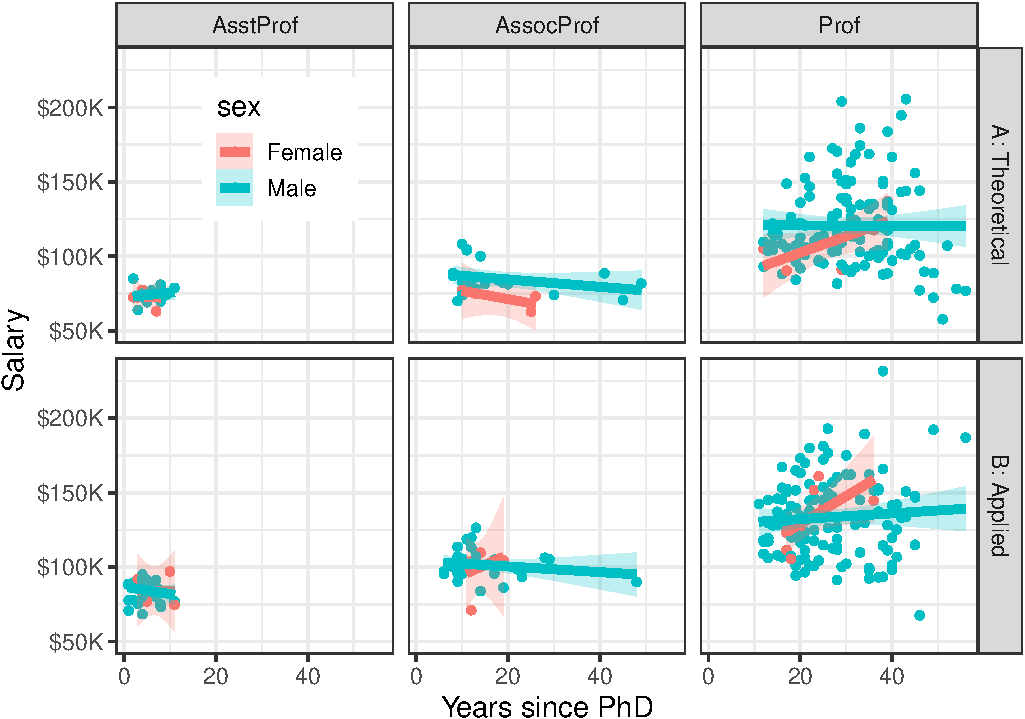
\includegraphics[width=1\textwidth,height=\textheight]{figs/ch03/fig-Salaries-facet-sex-1.pdf}

}

\caption{\label{fig-Salaries-facet-sex}Scatterplot of Salary vs.~years
since PhD, grouped by sex, faceted by discipline and rank.}

\end{figure}

\hypertarget{sec-data-ellipse}{%
\subsection{Data Ellipses}\label{sec-data-ellipse}}

The \emph{data ellipse} (\protect\hyperlink{ref-Monette:90}{Monette,
1990}), or \emph{concentration ellipse}
(\protect\hyperlink{ref-Dempster:69}{Dempster, 1969}) is a remarkably
simple and effective display for viewing and understanding bivariate
relationships in multivariate data. The data ellipse is typically used
to add a visual summary to a scatterplot, that shows all together the
means, standard deviations, correlation, and slope of the regression
line for two variables, perhaps stratified by another variable. Under
the classical assumption that the data are bivariate normally
distributed, the data ellipse is also a \textbf{sufficient} visual
summary, in the sense that it captures \textbf{all} relevant features of
the data. See Friendly et al.
(\protect\hyperlink{ref-Friendly-etal:ellipses:2013}{2013}) for a
complete discussion of the role of ellipsoids in statistical data
visualization.

It is based on the idea that in a bivariate normal distribution, the
contours of equal probability form a series of concentric ellipses. If
the variables were uncorrelated and had the same variances, these would
be circles, and Euclidean distance would measure the distance of each
observation from the mean. When the variables are correlated, a
different measure, \emph{Mahalanobis distance} is the proper measure of
how far a point is from the mean, taking the correlation into account.

\begin{figure}

{\centering 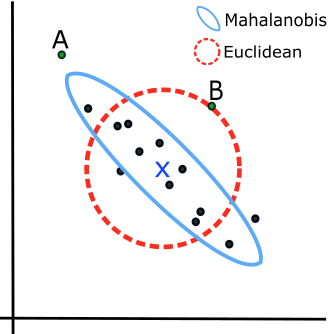
\includegraphics[width=0.6\textwidth,height=\textheight]{images/mahalanobis.png}

}

\caption{\label{fig-mahalanobis}2D data with curves of constant distance
from the centroid. The blue solid ellipse shows a contour of constant
Mahalanobis distance, taking the correlation into account; the dashed
red circle is a contour of equal Euclidean distance. Given the data
points, Which of the points \textbf{A} and \textbf{B} is further from
the mean (X)? \emph{Source}: Re-drawn from
\href{https://ouzhang.rbind.io/2020/11/16/outliers-part4/}{Ou Zhang}}

\end{figure}

To illustrate, Figure~\ref{fig-mahalanobis} shows a scatterplot with
labels for two points, ``A'' and ``B''. Which is further from the mean,
``X''? A contour of constant Euclidean distance, shown by the red dashed
circle, ignores the apparent negative correlation, so point ``A'' is
further. The blue ellipse for Mahalanobis distance takes the correlation
into account, so point ``B'' has a greater distance from the mean.

Mathematically, Euclidean (squared) distance for \(p\) variables,
\(j = 1, 2, \dots , p\), is just a generalization of the square of a
univariate standardized (\(z\)) score, \(z^2 = [(y - \bar{y}) / s]^2\),

\[
D_E^2 (\mathbf{y}) = \sum_j^p z_j^2 = \mathbf{z}^T  \mathbf{z} = (\mathbf{y} - \bar{\mathbf{y}})^T \operatorname{diag}(\mathbf{S})^{-1} (\mathbf{y} - \bar{\mathbf{y}}) \; ,
\] where \(\mathbf{S}\) is the sample variance-covariance matrix,
\(\mathbf{S} = ({n-1})^{-1} \sum_{i=1}^n (\mathbf{y}_i - \bar{\mathbf{y}})^T (\mathbf{y}_i - \bar{\mathbf{y}})\).

Mahalanobis' distance takes the correlations into account simply by
using the covariances as well as the variances, \[
D_M^2 (\mathbf{y}) = (\mathbf{y} - \bar{\mathbf{y}})^T S^{-1} (\mathbf{y} - \bar{\mathbf{y}}) \; .
\] For \(p\) variables, the data \emph{ellipsoid} \(\mathcal{E}_c\) of
size \(c\) is a \(p\)-dimensional ellipse, defined as the set of points
\(\mathbf{y} = (y_1, y_2, \dots y_p)\) whose squared Mahalanobis
distance, \(D_M^2 ( \mathbf{y} )\) is less than or equal to \(c^2\).

When \(\mathbf{y}\) is (at least approximately) bivariate normal,
\(D_M^2(\mathbf{y})\) has a large-sample \(\chi^2_2\) distribution
(\(\chi^2\) with 2 df), so taking \(c^2 = \chi^2_2 (0.68) = 2.28\) gives
a ``1 standard deviation bivariate ellipse,'' an analog of the standard
interval \(\bar{y} \pm 1 s\), while
\(c^2 = \chi^2_2 (0.95) = 5.99 \approx 6\) gives a data ellipse of 95\%
coverage.

\hypertarget{properties}{%
\subsubsection{Properties}\label{properties}}

The essential ideas of correlation and regression and their relation to
ellipses go back to Galton (\protect\hyperlink{ref-Galton:1886}{1886}).
Galton's goal was to predict (or explain) how a heritable trait, \(Y\),
(e.g., height) of children was related to that of their parents, \(X\).
He made a semi-graphic table of the frequencies of 928 observations of
the average height of father and mother versus the height of their
child, shown in Figure~\ref{fig-galton-corr}. He then drew smoothed
contour lines of equal frequencies and had the wonderful visual insight
that these formed concentric shapes that were tolerably close to
ellipses. He then calculated summaries, \(\text{Ave}(Y | X)\), and, for
symmetry, \(\text{Ave}(X | Y)\), and plotted these as lines of means on
his diagram. Lo and behold, he had a second visual insight: the lines of
means of (\(Y | X\)) and (\(X | Y\)) corresponded approximately to the
loci of horizontal and vertical tangents to the concentric ellipses. To
complete the picture, he added lines showing the major and minor axes of
the family of ellipses (which turned out to be the principal components)
with the result shown in Figure~\ref{fig-galton-corr}.

\begin{figure}

{\centering 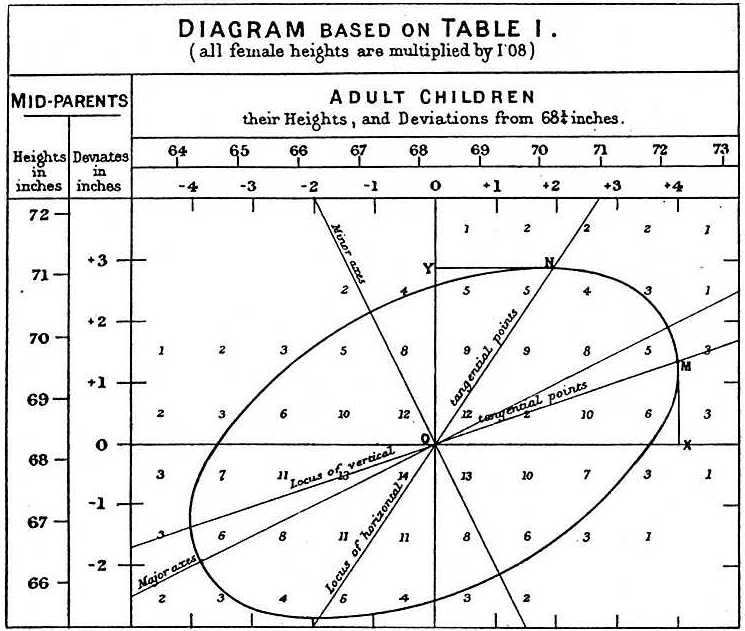
\includegraphics[width=0.7\textwidth,height=\textheight]{images/galton-corr.jpg}

}

\caption{\label{fig-galton-corr}Galton's 1886 diagram, showing the
relationship of height of children to the average of their parents'
height. The diagram is essentially an overlay of a geometrical
interpretation on a bivariate grouped frequency distribution, shown as
numbers.}

\end{figure}

For two variables, \(x\) and \(y\), the remarkable properties of the
data ellipse are illustrated in Figure~\ref{fig-galton-ellipse-r}, a
modern reconstruction of Galton's diagram.

\begin{figure}

{\centering 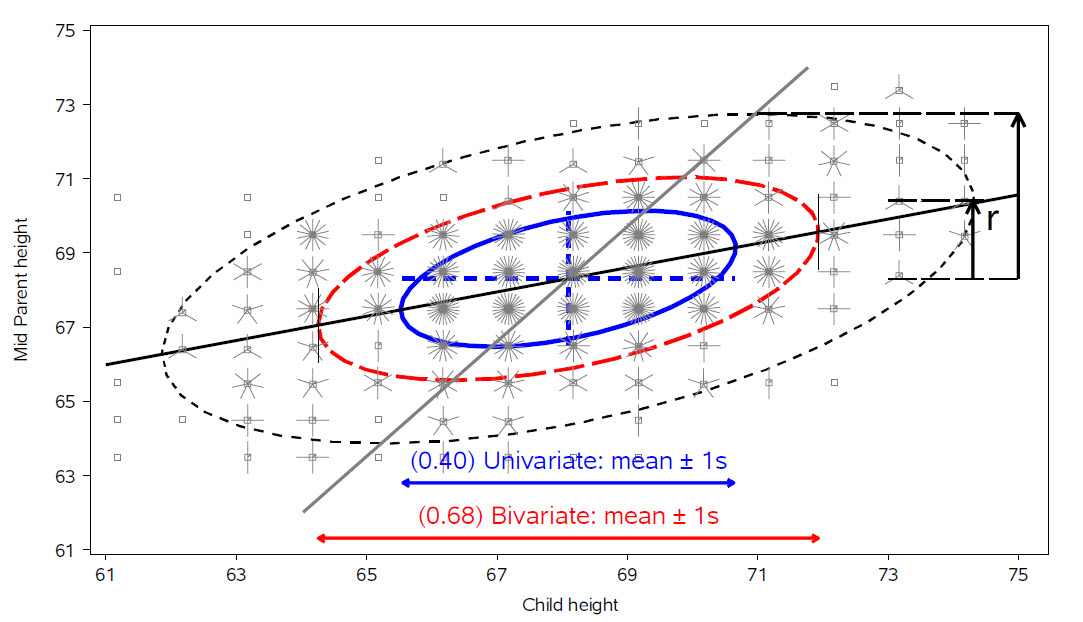
\includegraphics[width=1\textwidth,height=\textheight]{images/galton-ellipse-r.jpg}

}

\caption{\label{fig-galton-ellipse-r}Sunflower plot of Galton's data on
heights of parents and their children (in.), with 40\%, 68\% and 95\%
data ellipses and the regression lines of \(y\) on \(x\) (black) and
\(x\) on \(y\) (grey).}

\end{figure}

\begin{itemize}
\item
  The ellipses have the mean vector \((\bar{x}, \bar{y})\) as their
  center.
\item
  The lengths of arms of the central cross show the standard deviations
  of the variables, which correspond to the shadows of the ellipse
  covering 40\% of the data. These are the bivariate analogs of the
  standard intervals \(\bar{x} \pm 1 s_x\) and \(\bar{y} \pm 1 s_y\).
\item
  More generally, shadows (projections) on the coordinate axes, or any
  linear combination of them, give any standard interval,
  \(\bar{x} \pm k s_x\) and \(\bar{y} \pm k s_y\). Those with
  \(k=1, 1.5, 2.45\), have bivariate coverage 40\%, 68\% and 95\%
  respectively, corresponding to these quantiles of the \(\chi^2\)
  distribution with 2 degrees of freedom, i.e.,
  \(\chi^2_2 (.40) \approx 1^2\), \(\chi^2_2 (.68) \approx 1.5^2\), and
  \(\chi^2_2 (.95) \approx 2.45\). The shadows of the 68\% ellipse are
  the bivariate analog of a univariate \(\bar{x} \pm 1 s_x\) interval.
\item
  The regression line predicting \(y\) from \(x\) goes through the
  points where the ellipses have vertical tangents. The \emph{other}
  regression line, predicting \(x\) from \(y\) goes through the points
  of horizontal tangency.
\item
  The correlation \(r(x, y)\) is the ratio of the vertical segment from
  the mean of \(y\) to the regression line to the vertical segment going
  to the top of the ellipse as shown at the right of the figure. It is
  \(r = 0.46\) in this example.
\item
  The residual standard deviation,
  \(s_e = \sqrt{MSE} = \sqrt{\Sigma (y - \bar{y})^2 / n-2}\), is the
  half-length of the ellipse at the mean \(\bar{x}\).
\end{itemize}

Because Galton's values of \texttt{parent} and \texttt{child} height
were recorded in class intervals of 1 in., they are shown as sunflower
symbols in Figure~\ref{fig-galton-ellipse-r}, with multiple `petals'
reflecting the number of observations at each location. This plot
(except for annotations) is constructed using \texttt{sunflowerplot()}
and \texttt{car::dataEllipse()} for the ellipses.

\begin{Shaded}
\begin{Highlighting}[]
\FunctionTok{data}\NormalTok{(Galton, }\AttributeTok{package =} \StringTok{"HistData"}\NormalTok{)}

\FunctionTok{sunflowerplot}\NormalTok{(parent }\SpecialCharTok{\textasciitilde{}}\NormalTok{ child, }\AttributeTok{data=}\NormalTok{Galton, }
      \AttributeTok{xlim=}\FunctionTok{c}\NormalTok{(}\DecValTok{61}\NormalTok{,}\DecValTok{75}\NormalTok{), }
      \AttributeTok{ylim=}\FunctionTok{c}\NormalTok{(}\DecValTok{61}\NormalTok{,}\DecValTok{75}\NormalTok{), }
      \AttributeTok{seg.col=}\StringTok{"black"}\NormalTok{, }
        \AttributeTok{xlab=}\StringTok{"Child height"}\NormalTok{, }
      \AttributeTok{ylab=}\StringTok{"Mid Parent height"}\NormalTok{)}

\NormalTok{y.x }\OtherTok{\textless{}{-}} \FunctionTok{lm}\NormalTok{(parent }\SpecialCharTok{\textasciitilde{}}\NormalTok{ child, }\AttributeTok{data=}\NormalTok{Galton)     }\CommentTok{\# regression of y on x}
\FunctionTok{abline}\NormalTok{(y.x, }\AttributeTok{lwd=}\DecValTok{2}\NormalTok{)}
\NormalTok{x.y }\OtherTok{\textless{}{-}} \FunctionTok{lm}\NormalTok{(child }\SpecialCharTok{\textasciitilde{}}\NormalTok{ parent, }\AttributeTok{data=}\NormalTok{Galton)     }\CommentTok{\# regression of x on y}
\NormalTok{cc }\OtherTok{\textless{}{-}} \FunctionTok{coef}\NormalTok{(x.y)}
\FunctionTok{abline}\NormalTok{(}\SpecialCharTok{{-}}\NormalTok{cc[}\DecValTok{1}\NormalTok{]}\SpecialCharTok{/}\NormalTok{cc[}\DecValTok{2}\NormalTok{], }\DecValTok{1}\SpecialCharTok{/}\NormalTok{cc[}\DecValTok{2}\NormalTok{], }\AttributeTok{lwd=}\DecValTok{2}\NormalTok{, }\AttributeTok{col=}\StringTok{"gray"}\NormalTok{)}

\FunctionTok{with}\NormalTok{(Galton, }
\NormalTok{     car}\SpecialCharTok{::}\FunctionTok{dataEllipse}\NormalTok{(child, parent, }
         \AttributeTok{plot.points=}\ConstantTok{FALSE}\NormalTok{, }
         \AttributeTok{levels=}\FunctionTok{c}\NormalTok{(}\FloatTok{0.40}\NormalTok{, }\FloatTok{0.68}\NormalTok{, }\FloatTok{0.95}\NormalTok{), }
         \AttributeTok{lty=}\DecValTok{1}\SpecialCharTok{:}\DecValTok{3}\NormalTok{)}
\NormalTok{    )}
\end{Highlighting}
\end{Shaded}

\hypertarget{r-functions-for-data-ellipses}{%
\subsubsection{R functions for data
ellipses}\label{r-functions-for-data-ellipses}}

A number of packages provide functions for drawing data ellipses in a
scatterplot, with various features.

\begin{itemize}
\tightlist
\item
  \texttt{car::scatterplot()}: uses base R graphics to draw 2D
  scatterplots, with a wide variety of plot enhancements including
  linear and non-parametric smoothers (loess, gam), a formula method,
  e.g., \texttt{y\ \textasciitilde{}\ x\ \textbar{}\ group}, and marking
  points and lines using symbol shape, color, etc. Importantly, the
  \textbf{car} package generally allows automatic identification of
  ``noteworthy'' points by their labels in the plot using a variety of
  methods. For example, \texttt{method\ =\ "mahal"} labels cases with
  the most extreme Mahalanobis distances; \texttt{method\ =\ "r"}
  selects points according to their value of \texttt{abs(y)}, which is
  appropriate in residual plots.
\item
  \texttt{car::dataEllipse()}: plots classical or robust data (using
  \texttt{MASS::cov/trob()}) ellipses for one or more groups, with the
  same facilities for point identification.
\item
  \texttt{heplots::covEllipses()}: draws classical or robust data
  ellipses for one or more groups in a one-way design and optionally for
  the pooled total sample, where the focus is on homogeneity of
  within-group covariance matrices.
\item
  \texttt{ggplot2::stat\_ellipse()}: uses the calculation methods of
  \texttt{car::dataEllipse()} to add unfilled (\texttt{geom\ =\ "path"})
  or filled (\texttt{geom\ =\ polygon"}) data ellipses in a
  \texttt{ggplot} scatterplot, using inherited aesthetics.
\end{itemize}

\hypertarget{sec-prestige}{%
\subsubsection{Example: Canadian occupational
prestige}\label{sec-prestige}}

These examples use the data on the prestige of 102 occupational
categories and other measures from the 1971 Canadian Census, recorded in
\texttt{carData::Prestige}. Our interest is in understanding how
\texttt{prestige} (the Pineo-Porter
(\protect\hyperlink{ref-PineoPorter2008}{Pineo \& Porter, 2008})
prestige score for an occupational category, derived from a social
survey) is related to census measures of the average education, income,
percent women of incumbents in those occupations. Occupation
\texttt{type} is a factor with levels \texttt{"bc"} (blue collar),
\texttt{"wc"} (white collar) and \texttt{"prof"} (professional).

\begin{Shaded}
\begin{Highlighting}[]
\FunctionTok{data}\NormalTok{(Prestige, }\AttributeTok{package=}\StringTok{"carData"}\NormalTok{)}
\CommentTok{\# \textasciigrave{}type\textasciigrave{} is really an ordered factor. Make it so.}
\NormalTok{Prestige}\SpecialCharTok{$}\NormalTok{type }\OtherTok{\textless{}{-}} \FunctionTok{ordered}\NormalTok{(Prestige}\SpecialCharTok{$}\NormalTok{type,}
                         \AttributeTok{levels=}\FunctionTok{c}\NormalTok{(}\StringTok{"bc"}\NormalTok{, }\StringTok{"wc"}\NormalTok{, }\StringTok{"prof"}\NormalTok{))}
\FunctionTok{str}\NormalTok{(Prestige)}
\CommentTok{\#\textgreater{} \textquotesingle{}data.frame\textquotesingle{}:    102 obs. of  6 variables:}
\CommentTok{\#\textgreater{}  $ education: num  13.1 12.3 12.8 11.4 14.6 ...}
\CommentTok{\#\textgreater{}  $ income   : int  12351 25879 9271 8865 8403 11030 8258 14163 11377 11023 ...}
\CommentTok{\#\textgreater{}  $ women    : num  11.16 4.02 15.7 9.11 11.68 ...}
\CommentTok{\#\textgreater{}  $ prestige : num  68.8 69.1 63.4 56.8 73.5 77.6 72.6 78.1 73.1 68.8 ...}
\CommentTok{\#\textgreater{}  $ census   : int  1113 1130 1171 1175 2111 2113 2133 2141 2143 2153 ...}
\CommentTok{\#\textgreater{}  $ type     : Ord.factor w/ 3 levels "bc"\textless{}"wc"\textless{}"prof": 3 3 3 3 3 3 3 3 3 3 ...}
\end{Highlighting}
\end{Shaded}

I first illustrate the relation between \texttt{income} and
\texttt{prestige} using \texttt{car::scatterplot()} with many of its
bells and whistles, including marginal boxplots for the variables, the
linear regression line, loess smooth and the 68\% data ellipse.

\begin{Shaded}
\begin{Highlighting}[]
\FunctionTok{scatterplot}\NormalTok{(prestige }\SpecialCharTok{\textasciitilde{}}\NormalTok{ income, }\AttributeTok{data=}\NormalTok{Prestige,}
  \AttributeTok{pch =} \DecValTok{16}\NormalTok{, }\AttributeTok{cex.lab =} \FloatTok{1.25}\NormalTok{,}
  \AttributeTok{regLine =} \FunctionTok{list}\NormalTok{(}\AttributeTok{col =} \StringTok{"red"}\NormalTok{, }\AttributeTok{lwd=}\DecValTok{3}\NormalTok{),}
  \AttributeTok{smooth =} \FunctionTok{list}\NormalTok{(}\AttributeTok{smoother=}\NormalTok{loessLine, }
                \AttributeTok{lty.smooth =} \DecValTok{1}\NormalTok{, }\AttributeTok{lwd.smooth=}\DecValTok{3}\NormalTok{,}
                \AttributeTok{col.smooth =} \StringTok{"darkgreen"}\NormalTok{, }\AttributeTok{col.var =} \StringTok{"darkgreen"}\NormalTok{),}
  \AttributeTok{ellipse =} \FunctionTok{list}\NormalTok{(}\AttributeTok{levels =} \FloatTok{0.68}\NormalTok{),}
  \AttributeTok{id =} \FunctionTok{list}\NormalTok{(}\AttributeTok{n=}\DecValTok{4}\NormalTok{, }\AttributeTok{method =} \StringTok{"mahal"}\NormalTok{, }\AttributeTok{col=}\StringTok{"black"}\NormalTok{, }\AttributeTok{cex=}\FloatTok{1.2}\NormalTok{))}
\CommentTok{\#\textgreater{} general.managers          lawyers        ministers       physicians }
\CommentTok{\#\textgreater{}                2               17               20               24}
\end{Highlighting}
\end{Shaded}

\begin{figure}[H]

{\centering 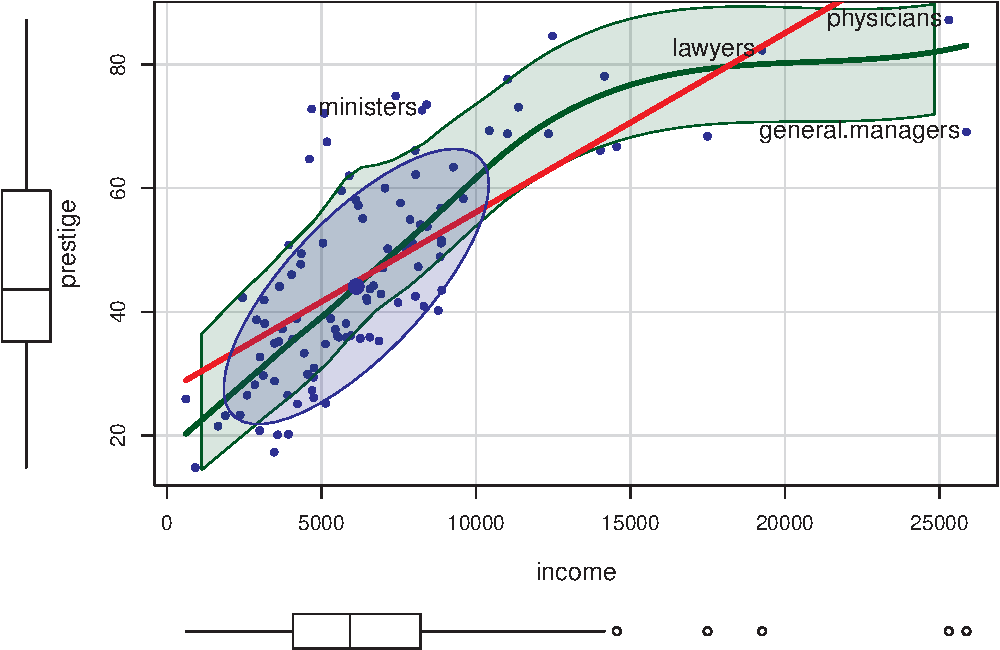
\includegraphics[width=0.8\textwidth,height=\textheight]{figs/ch03/fig-Prestige-scatterplot-income1-1.pdf}

}

\caption{\label{fig-Prestige-scatterplot-income1}Scatterplot of prestige
vs.~income, showing the linear regression line (red), the loess smooth
with a confidence envelope (darkgreen) and a 68\% data ellipse.}

\end{figure}

There is a lot that can be seen here:

\begin{itemize}
\tightlist
\item
  \texttt{income} is positively skewed, as is often the case.
\item
  The loess smooth, on the scale of income, shows \texttt{prestige}
  increasing up to \$15,000 (these are 1971 incomes), and then leveling
  off.
\item
  The data ellipse, centered at the means encloses approximately 68\% of
  the data points. It adds visual information about the correlation and
  precision of the linear regression; but here, the non-linear trend for
  higher incomes strongly suggests a different approach.
\item
  The four points identified by their labels are those with the largest
  Mahalanobis distances. \texttt{scatterplot()} prints their labels to
  the console.
\end{itemize}

Figure~\ref{fig-Prestige-scatterplot-educ1} shows a similar plot for
education, which from the boxplot appears to be reasonably symmetric.
The smoothed curve is quite close to the linear regression, according to
which \texttt{prestige} increases on average
\texttt{coef(lm(prestige\ \textasciitilde{}\ education,\ data=Prestige)){[}2{]}}
= 5.361 with each year of education.

\begin{Shaded}
\begin{Highlighting}[]
\FunctionTok{scatterplot}\NormalTok{(prestige }\SpecialCharTok{\textasciitilde{}}\NormalTok{ education, }\AttributeTok{data=}\NormalTok{Prestige,}
  \AttributeTok{pch =} \DecValTok{16}\NormalTok{, }\AttributeTok{cex.lab =} \FloatTok{1.25}\NormalTok{,}
  \AttributeTok{regLine =} \FunctionTok{list}\NormalTok{(}\AttributeTok{col =} \StringTok{"red"}\NormalTok{, }\AttributeTok{lwd=}\DecValTok{3}\NormalTok{),}
  \AttributeTok{smooth =} \FunctionTok{list}\NormalTok{(}\AttributeTok{smoother=}\NormalTok{loessLine, }
                \AttributeTok{lty.smooth =} \DecValTok{1}\NormalTok{, }\AttributeTok{lwd.smooth=}\DecValTok{3}\NormalTok{,}
                \AttributeTok{col.smooth =} \StringTok{"darkgreen"}\NormalTok{, }\AttributeTok{col.var =} \StringTok{"darkgreen"}\NormalTok{),}
  \AttributeTok{ellipse =} \FunctionTok{list}\NormalTok{(}\AttributeTok{levels =} \FloatTok{0.68}\NormalTok{),}
  \AttributeTok{id =} \FunctionTok{list}\NormalTok{(}\AttributeTok{n=}\DecValTok{4}\NormalTok{, }\AttributeTok{method =} \StringTok{"mahal"}\NormalTok{, }\AttributeTok{col=}\StringTok{"black"}\NormalTok{, }\AttributeTok{cex=}\FloatTok{1.2}\NormalTok{))}
\CommentTok{\#\textgreater{}  physicians file.clerks    newsboys     farmers }
\CommentTok{\#\textgreater{}          24          41          53          67}
\end{Highlighting}
\end{Shaded}

\begin{figure}

{\centering 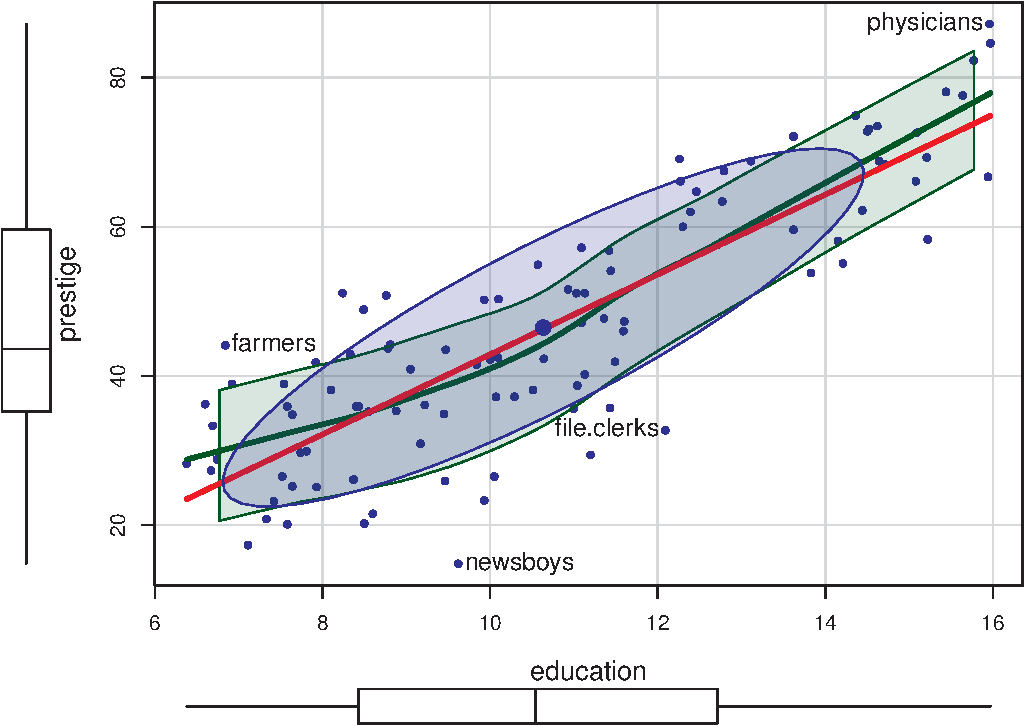
\includegraphics[width=0.8\textwidth,height=\textheight]{figs/ch03/fig-Prestige-scatterplot-educ1-1.pdf}

}

\caption{\label{fig-Prestige-scatterplot-educ1}Scatterplot of prestige
vs.~education, showing the linear regression line (red), the loess
smooth with a confidence envelope (darkgreen) and a 68\% data ellipse.}

\end{figure}

In this plot, farmers, newsboys, file.clerks and physicians are
identified as noteworthy, for being furthest from the mean by
Mahalanobis distance. In relation to their typical level of education,
these are mostly understandable, but it is nice that farmers are rated
of higher prestige than their level of education would predict.

Note that the \texttt{method} argument for point identification can take
a vector of case numbers indicating the points to be labeled. So, to
label the observations with large absolute standardized residuals in the
linear model \texttt{m}, you can use
\texttt{method\ =\ which(abs(rstandard(m))\ \textgreater{}\ 2)}.

\begin{Shaded}
\begin{Highlighting}[]
\NormalTok{m }\OtherTok{\textless{}{-}} \FunctionTok{lm}\NormalTok{(prestige }\SpecialCharTok{\textasciitilde{}}\NormalTok{ education, }\AttributeTok{data=}\NormalTok{Prestige)}
\FunctionTok{scatterplot}\NormalTok{(prestige }\SpecialCharTok{\textasciitilde{}}\NormalTok{ education, }\AttributeTok{data=}\NormalTok{Prestige,}
            \AttributeTok{pch =} \DecValTok{16}\NormalTok{, }\AttributeTok{cex.lab =} \FloatTok{1.25}\NormalTok{,}
            \AttributeTok{boxplots =} \ConstantTok{FALSE}\NormalTok{,}
            \AttributeTok{regLine =} \FunctionTok{list}\NormalTok{(}\AttributeTok{col =} \StringTok{"red"}\NormalTok{, }\AttributeTok{lwd=}\DecValTok{3}\NormalTok{),}
            \AttributeTok{smooth =} \FunctionTok{list}\NormalTok{(}\AttributeTok{smoother=}\NormalTok{loessLine,}
                          \AttributeTok{lty.smooth =} \DecValTok{1}\NormalTok{, }\AttributeTok{col.smooth =} \StringTok{"black"}\NormalTok{, }\AttributeTok{lwd.smooth=}\DecValTok{3}\NormalTok{,}
                          \AttributeTok{col.var =} \StringTok{"darkgreen"}\NormalTok{),}
            \AttributeTok{ellipse =} \FunctionTok{list}\NormalTok{(}\AttributeTok{levels =} \FloatTok{0.68}\NormalTok{),}
            \AttributeTok{id =} \FunctionTok{list}\NormalTok{(}\AttributeTok{n=}\DecValTok{4}\NormalTok{, }\AttributeTok{method =} \FunctionTok{which}\NormalTok{(}\FunctionTok{abs}\NormalTok{(}\FunctionTok{rstandard}\NormalTok{(m))}\SpecialCharTok{\textgreater{}}\DecValTok{2}\NormalTok{), }
                      \AttributeTok{col=}\StringTok{"black"}\NormalTok{, }\AttributeTok{cex=}\FloatTok{1.2}\NormalTok{)) }\SpecialCharTok{|\textgreater{}} \FunctionTok{invisible}\NormalTok{()}
\end{Highlighting}
\end{Shaded}

\begin{figure}

{\centering 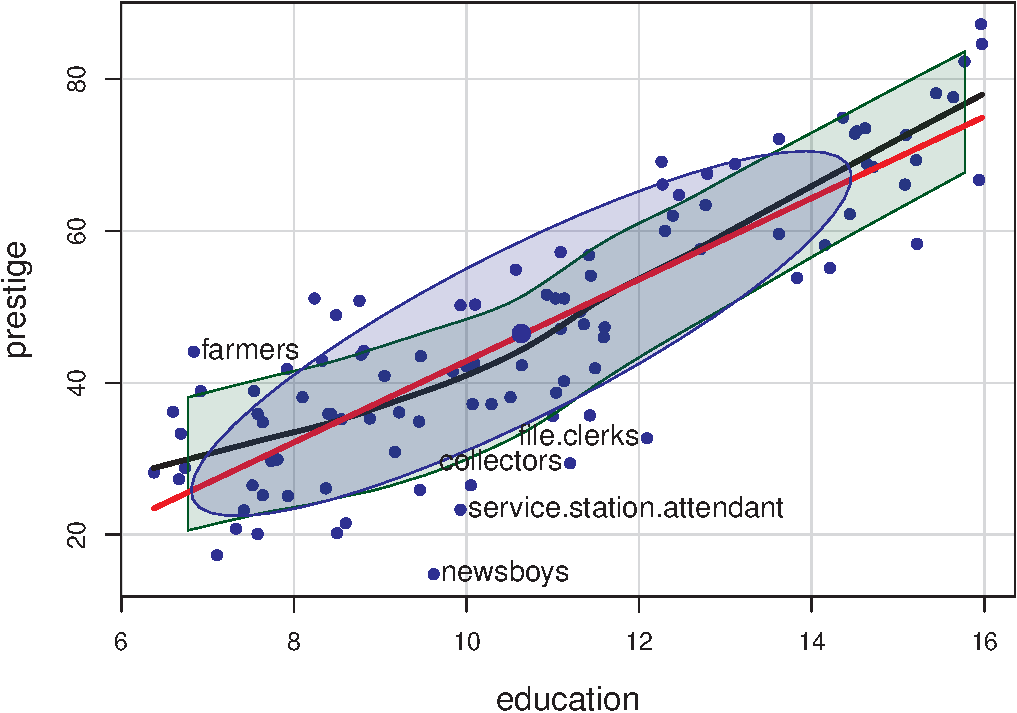
\includegraphics[width=0.8\textwidth,height=\textheight]{figs/ch03/fig-Prestige-scatterplot-educ2-1.pdf}

}

\caption{\label{fig-Prestige-scatterplot-educ2}Scatterplot of prestige
vs.~education, labeling points whose absolute stanardized residual is
\textgreater{} 2.}

\end{figure}

\hypertarget{sec-log-scale}{%
\subsubsection{Plotting on a log scale}\label{sec-log-scale}}

A typical remedy for the non-linear relationship of income to prestige
is to plot income on a log scale. This usually makes sense, and
expresses a belief that a \textbf{multiple} of or \textbf{percentage
increase} in income has a constant impact on prestige, as opposed to the
\textbf{additive} interpretation for income itself.

For example, the slope of the linear regression line in
Figure~\ref{fig-Prestige-scatterplot-income1} is given by
\texttt{coef(lm(prestige\ \textasciitilde{}\ income,\ data=Prestige)){[}2{]}}
= 0.003. Multiplying this by 1000 says that a \$1000 increase in
\texttt{income} is associated with with an average increase of
\texttt{prestige} of 2.9.

In the plot below, \texttt{scatterplot(...,\ log\ =\ "x")} re-scales the
x-axis to the \(\log_e()\) scale. The slope,
\texttt{coef(lm(prestige\ \textasciitilde{}\ log(income),\ data=Prestige)){[}2{]}}
= 21.556 says that a 1\% increase in salary is associated with an
average change of 21.55 / 100 in prestige.

\begin{Shaded}
\begin{Highlighting}[]
\FunctionTok{scatterplot}\NormalTok{(prestige }\SpecialCharTok{\textasciitilde{}}\NormalTok{ income, }\AttributeTok{data=}\NormalTok{Prestige,}
  \AttributeTok{log =} \StringTok{"x"}\NormalTok{,}
  \AttributeTok{pch =} \DecValTok{16}\NormalTok{, }\AttributeTok{cex.lab =} \FloatTok{1.25}\NormalTok{,}
  \AttributeTok{regLine =} \FunctionTok{list}\NormalTok{(}\AttributeTok{col =} \StringTok{"red"}\NormalTok{, }\AttributeTok{lwd=}\DecValTok{3}\NormalTok{),}
  \AttributeTok{smooth =} \FunctionTok{list}\NormalTok{(}\AttributeTok{smoother=}\NormalTok{loessLine,}
                \AttributeTok{lty.smooth =} \DecValTok{1}\NormalTok{, }\AttributeTok{lwd.smooth=}\DecValTok{3}\NormalTok{,}
                \AttributeTok{col.smooth =} \StringTok{"darkgreen"}\NormalTok{, }\AttributeTok{col.var =} \StringTok{"darkgreen"}\NormalTok{),}
  \AttributeTok{ellipse =} \FunctionTok{list}\NormalTok{(}\AttributeTok{levels =} \FloatTok{0.68}\NormalTok{),}
  \AttributeTok{id =} \FunctionTok{list}\NormalTok{(}\AttributeTok{n=}\DecValTok{4}\NormalTok{, }\AttributeTok{method =} \StringTok{"mahal"}\NormalTok{, }\AttributeTok{col=}\StringTok{"black"}\NormalTok{, }\AttributeTok{cex=}\FloatTok{1.2}\NormalTok{))}
\CommentTok{\#\textgreater{} general.managers        ministers         newsboys      babysitters }
\CommentTok{\#\textgreater{}                2               20               53               63}
\end{Highlighting}
\end{Shaded}

\begin{figure}

{\centering 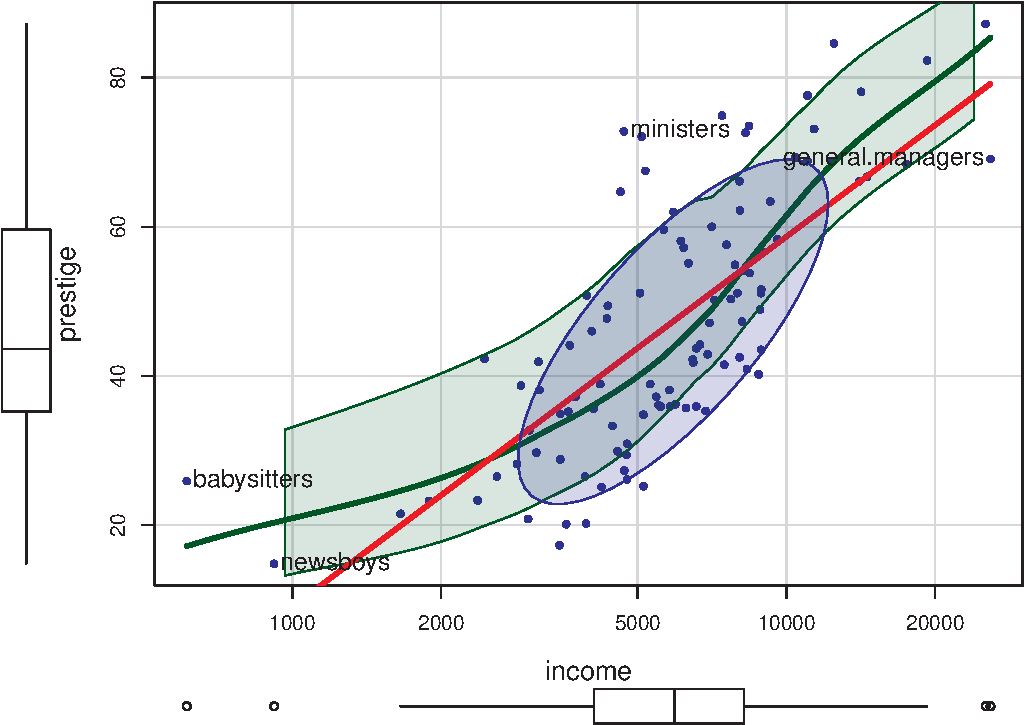
\includegraphics[width=0.8\textwidth,height=\textheight]{figs/ch03/fig-Prestige-scatterplot2-1.pdf}

}

\caption{\label{fig-Prestige-scatterplot2}Scatterplot of prestige
vs.~log(income).}

\end{figure}

The smoothed curve in Figure~\ref{fig-Prestige-scatterplot2} exhibits a
slight tendency to bend upwards, but a linear relation is a reasonable
approximation.

\hypertarget{stratifying}{%
\subsubsection{Stratifying}\label{stratifying}}

Before going further, it is instructive to ask what we could see in the
relationship between income and prestige if we stratified by type of
occupation, fitting separate regressions and smooths for blue collar,
white collar and professional incumbents in these occupations.

The formula
\texttt{prestige\ \textasciitilde{}\ income\ \textbar{}\ type} is a
natural way to specify grouping by \texttt{type}; separate linear
regressions and smooths are calculated for each group, applying the
color and point shapes specified by the \texttt{col} and \texttt{pch}
arguments.

\begin{Shaded}
\begin{Highlighting}[]
\FunctionTok{scatterplot}\NormalTok{(prestige }\SpecialCharTok{\textasciitilde{}}\NormalTok{ income }\SpecialCharTok{|}\NormalTok{ type, }\AttributeTok{data=}\NormalTok{Prestige,}
  \AttributeTok{col =} \FunctionTok{c}\NormalTok{(}\StringTok{"blue"}\NormalTok{, }\StringTok{"red"}\NormalTok{, }\StringTok{"darkgreen"}\NormalTok{),}
  \AttributeTok{pch =} \DecValTok{15}\SpecialCharTok{:}\DecValTok{17}\NormalTok{,}
  \AttributeTok{grid =} \ConstantTok{FALSE}\NormalTok{,}
  \AttributeTok{legend =} \FunctionTok{list}\NormalTok{(}\AttributeTok{coords=}\StringTok{"bottomright"}\NormalTok{),}
  \AttributeTok{regLine =} \FunctionTok{list}\NormalTok{(}\AttributeTok{lwd=}\DecValTok{3}\NormalTok{),}
  \AttributeTok{smooth=}\FunctionTok{list}\NormalTok{(}\AttributeTok{smoother=}\NormalTok{loessLine, }
              \AttributeTok{var=}\ConstantTok{FALSE}\NormalTok{, }\AttributeTok{lwd.smooth=}\DecValTok{2}\NormalTok{, }\AttributeTok{lty.smooth=}\DecValTok{1}\NormalTok{))}
\end{Highlighting}
\end{Shaded}

\begin{figure}[H]

{\centering 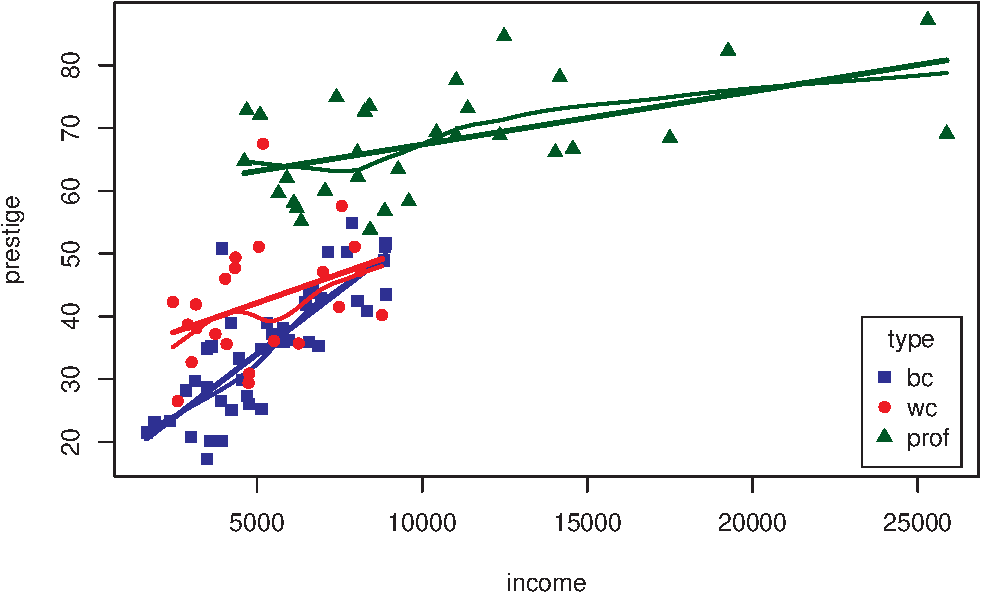
\includegraphics[width=0.8\textwidth,height=\textheight]{figs/ch03/fig-Prestige-scatterplot3-1.pdf}

}

\caption{\label{fig-Prestige-scatterplot3}Scatterplot of prestige
vs.~income, stratified by occupational type. This implies a different
interpretation, where occupation type is a moderator variable.}

\end{figure}

This visual analysis offers a different interpretation of the dependence
of prestige on income, which appeared to be non-linear when occupation
type was ignored. Instead, Figure~\ref{fig-Prestige-scatterplot3}
suggests an \emph{interaction} of income by type. In a model formula
this would be expressed as one of:

\begin{Shaded}
\begin{Highlighting}[]
\FunctionTok{lm}\NormalTok{(prestige }\SpecialCharTok{\textasciitilde{}}\NormalTok{ income }\SpecialCharTok{+}\NormalTok{ type }\SpecialCharTok{+}\NormalTok{ income}\SpecialCharTok{:}\NormalTok{type, }\AttributeTok{data =}\NormalTok{ Prestige)}
\FunctionTok{lm}\NormalTok{(prestige }\SpecialCharTok{\textasciitilde{}}\NormalTok{ income }\SpecialCharTok{*}\NormalTok{ type, }\AttributeTok{data =}\NormalTok{ Prestige)}
\end{Highlighting}
\end{Shaded}

These models signify that there are different slopes (and intercepts)
for the three occupational types. In this interpretation, \texttt{type}
is a moderator variable, with a different story. The slopes of the
fitted lines suggest that among blue collar workers, prestige increases
sharply with their income. For white collar and professional workers,
there is still an increasing relation of prestige with income, but the
effect of income (slope) diminishes with higher occupational category. A
different plot entails a different story.

\hypertarget{sec-penguins}{%
\subsubsection{Example: Penguins data}\label{sec-penguins}}

\begin{figure}

{\centering 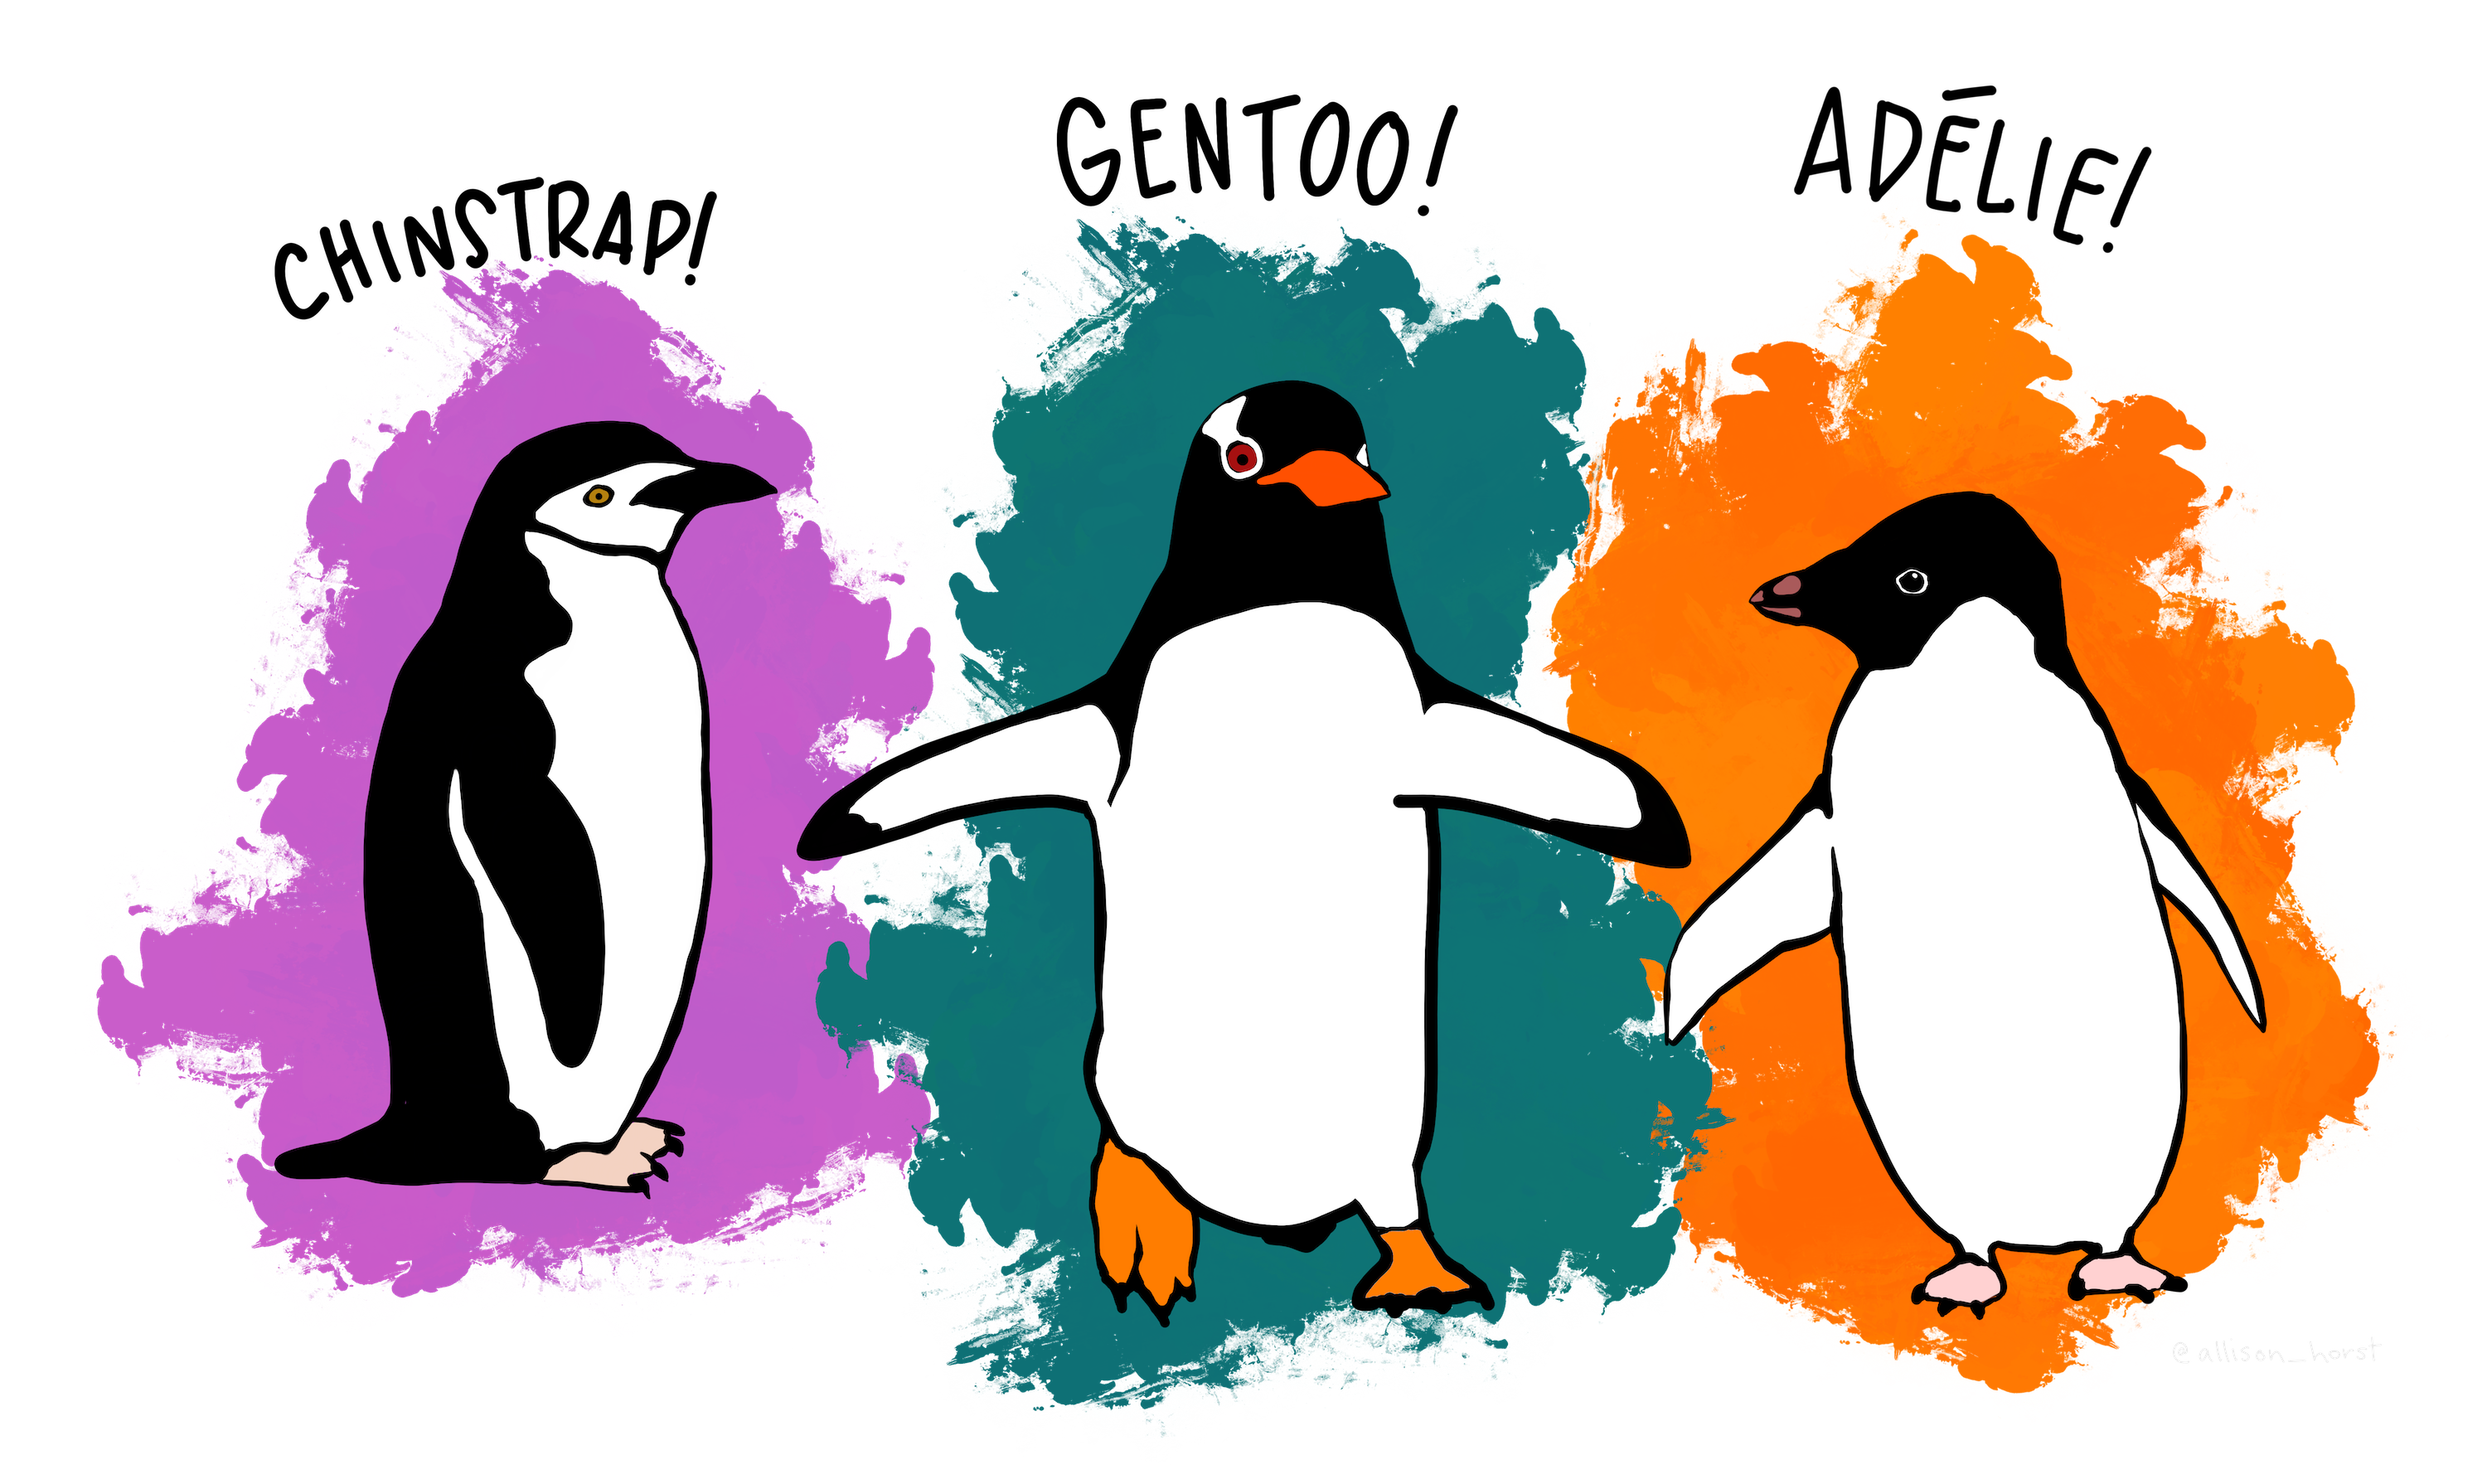
\includegraphics[width=0.8\textwidth,height=\textheight]{images/penguins-horst.png}

}

\caption{\label{fig-penguin-species}Penguin species observed in the
Palmer Archipelago. This is a cartoon, but it illustrates some features
of penguin body size measurements, and the colors typically used for
species. Image: Allison Horst}

\end{figure}

The \texttt{penguins} dataset from the \textbf{palmerpenguins} package
(\protect\hyperlink{ref-R-palmerpenguins}{Horst et al., 2022}) provides
further instructive examples of plots and analyses of multivariate data.
The data consists of measurements of body size (flipper length, body
mass, bill length and depth) of 344 penguins collected at the
\href{https://pallter.marine.rutgers.edu/}{Palmer Research Station} in
Antarctica.

There were three different species of penguins (Adélie, Chinstrap \&
Gentoo) collected from 3 islands in the Palmer Archipelago between
2007--2009 (\protect\hyperlink{ref-Gorman2014}{Gorman et al., 2014}).
The purpose was to examine differences in size or appearance of these
species, particularly differences among the sexes (sexual dimorphism) in
relation to foraging and habitat.

Here, I use a slightly altered version of the dataset, \texttt{peng},
renaming variables to remove the units, making factors of character
variables and deleting a few cases with missing data.

\begin{Shaded}
\begin{Highlighting}[]
\FunctionTok{data}\NormalTok{(penguins, }\AttributeTok{package =} \StringTok{"palmerpenguins"}\NormalTok{)}
\NormalTok{peng }\OtherTok{\textless{}{-}}\NormalTok{ penguins }\SpecialCharTok{|\textgreater{}}
  \FunctionTok{rename}\NormalTok{(}
    \AttributeTok{bill\_length =}\NormalTok{ bill\_length\_mm, }
    \AttributeTok{bill\_depth =}\NormalTok{ bill\_depth\_mm, }
    \AttributeTok{flipper\_length =}\NormalTok{ flipper\_length\_mm, }
    \AttributeTok{body\_mass =}\NormalTok{ body\_mass\_g}
\NormalTok{  ) }\SpecialCharTok{|\textgreater{}}
  \FunctionTok{mutate}\NormalTok{(}\AttributeTok{species =} \FunctionTok{as.factor}\NormalTok{(species),}
         \AttributeTok{island =} \FunctionTok{as.factor}\NormalTok{(island),}
         \AttributeTok{sex =} \FunctionTok{as.factor}\NormalTok{(}\FunctionTok{substr}\NormalTok{(sex,}\DecValTok{1}\NormalTok{,}\DecValTok{1}\NormalTok{))) }\SpecialCharTok{|\textgreater{}}
\NormalTok{  tidyr}\SpecialCharTok{::}\FunctionTok{drop\_na}\NormalTok{()}

\FunctionTok{str}\NormalTok{(peng)}
\CommentTok{\#\textgreater{} tibble [333 x 8] (S3: tbl\_df/tbl/data.frame)}
\CommentTok{\#\textgreater{}  $ species       : Factor w/ 3 levels "Adelie","Chinstrap",..: 1 1 1 1 1 1 1 1 1 1 ...}
\CommentTok{\#\textgreater{}  $ island        : Factor w/ 3 levels "Biscoe","Dream",..: 3 3 3 3 3 3 3 3 3 3 ...}
\CommentTok{\#\textgreater{}  $ bill\_length   : num [1:333] 39.1 39.5 40.3 36.7 39.3 38.9 39.2 41.1 38.6 34.6 ...}
\CommentTok{\#\textgreater{}  $ bill\_depth    : num [1:333] 18.7 17.4 18 19.3 20.6 17.8 19.6 17.6 21.2 21.1 ...}
\CommentTok{\#\textgreater{}  $ flipper\_length: int [1:333] 181 186 195 193 190 181 195 182 191 198 ...}
\CommentTok{\#\textgreater{}  $ body\_mass     : int [1:333] 3750 3800 3250 3450 3650 3625 4675 3200 3800 4400 ...}
\CommentTok{\#\textgreater{}  $ sex           : Factor w/ 2 levels "f","m": 2 1 1 1 2 1 2 1 2 2 ...}
\CommentTok{\#\textgreater{}  $ year          : int [1:333] 2007 2007 2007 2007 2007 2007 2007 2007 2007 2007 ...}
\end{Highlighting}
\end{Shaded}

There are quite a few variables to choose for illustrating data ellipses
in scatterplots. Here I focus on the measures of their bills,
\texttt{bill\_length} and \texttt{bill\_depth} (indicating curvature)
and show how to use \texttt{ggplot2} for these plots.

I'll be using the penguins data quite a lot, so it is useful to set up
custom colors like those used in Figure~\ref{fig-penguin-species}, and
shown in Figure~\ref{fig-peng-colors} with their color codes. These are
shades of:

\begin{itemize}
\tightlist
\item
  \textcolor{orange}{Adelie}: \textcolor{orange}{orange},
\item
  \textcolor{purple}{Chinstrap}: \textcolor{purple}{purple}, and
\item
  \textcolor{green}{Gentoo}: \textcolor{green}{green}.
\end{itemize}

\begin{figure}

{\centering 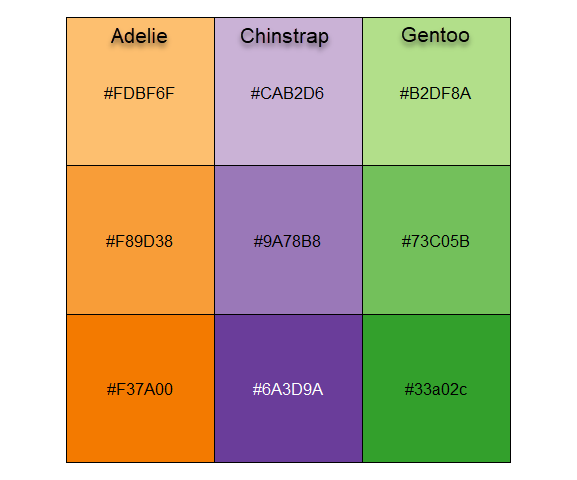
\includegraphics[width=0.7\textwidth,height=\textheight]{images/peng-colors.png}

}

\caption{\label{fig-peng-colors}Color palettes used for penguin
species.}

\end{figure}

To use these in \texttt{ggplot2} I define a function
\texttt{peng.colors()} that allows shades of light, medium and dark and
then functions \texttt{scale\_*\_penguins()} for color and fill.

\begin{Shaded}
\begin{Highlighting}[]
\NormalTok{peng.colors }\OtherTok{\textless{}{-}} \ControlFlowTok{function}\NormalTok{(}\AttributeTok{shade=}\FunctionTok{c}\NormalTok{(}\StringTok{"medium"}\NormalTok{, }\StringTok{"light"}\NormalTok{, }\StringTok{"dark"}\NormalTok{)) \{}
\NormalTok{  shade }\OtherTok{=} \FunctionTok{match.arg}\NormalTok{(shade)}
  \CommentTok{\#             light      medium     dark}
\NormalTok{  oranges }\OtherTok{\textless{}{-}} \FunctionTok{c}\NormalTok{(}\StringTok{"\#FDBF6F"}\NormalTok{, }\StringTok{"\#F89D38"}\NormalTok{, }\StringTok{"\#F37A00"}\NormalTok{)  }\CommentTok{\# Adelie}
\NormalTok{  purples }\OtherTok{\textless{}{-}} \FunctionTok{c}\NormalTok{(}\StringTok{"\#CAB2D6"}\NormalTok{, }\StringTok{"\#9A78B8"}\NormalTok{, }\StringTok{"\#6A3D9A"}\NormalTok{)  }\CommentTok{\# Chinstrap}
\NormalTok{  greens }\OtherTok{\textless{}{-}}  \FunctionTok{c}\NormalTok{(}\StringTok{"\#B2DF8A"}\NormalTok{, }\StringTok{"\#73C05B"}\NormalTok{, }\StringTok{"\#33a02c"}\NormalTok{)  }\CommentTok{\# Gentoo}
  
\NormalTok{  cols.vec }\OtherTok{\textless{}{-}} \FunctionTok{c}\NormalTok{(oranges, purples, greens)}
\NormalTok{  cols.mat }\OtherTok{\textless{}{-}} 
    \FunctionTok{matrix}\NormalTok{(cols.vec, }\DecValTok{3}\NormalTok{, }\DecValTok{3}\NormalTok{, }
           \AttributeTok{byrow =} \ConstantTok{TRUE}\NormalTok{,}
           \AttributeTok{dimnames =} \FunctionTok{list}\NormalTok{(}\AttributeTok{species =} \FunctionTok{c}\NormalTok{(}\StringTok{"Adelie"}\NormalTok{, }\StringTok{"Chinstrap"}\NormalTok{, }\StringTok{"Gentoo"}\NormalTok{),}
                           \AttributeTok{shade =} \FunctionTok{c}\NormalTok{(}\StringTok{"light"}\NormalTok{, }\StringTok{"medium"}\NormalTok{, }\StringTok{"dark"}\NormalTok{)))}
  \CommentTok{\# get shaded colors}
\NormalTok{  cols.mat[, shade ]}
\NormalTok{\}}

\CommentTok{\# define color and fill scales}
\NormalTok{scale\_fill\_penguins }\OtherTok{\textless{}{-}} \ControlFlowTok{function}\NormalTok{(}\AttributeTok{shade=}\FunctionTok{c}\NormalTok{(}\StringTok{"medium"}\NormalTok{, }\StringTok{"light"}\NormalTok{, }\StringTok{"dark"}\NormalTok{), ...)\{}
\NormalTok{  shade }\OtherTok{=} \FunctionTok{match.arg}\NormalTok{(shade)}
\NormalTok{  ggplot2}\SpecialCharTok{::}\FunctionTok{discrete\_scale}\NormalTok{(}
    \StringTok{"fill"}\NormalTok{,}\StringTok{"penguins"}\NormalTok{,}
\NormalTok{     scales}\SpecialCharTok{:::}\FunctionTok{manual\_pal}\NormalTok{(}\AttributeTok{values =} \FunctionTok{peng.colors}\NormalTok{(shade)), ...)}
\NormalTok{\}}

\NormalTok{scale\_colour\_penguins }\OtherTok{\textless{}{-}} \ControlFlowTok{function}\NormalTok{(}\AttributeTok{shade=}\FunctionTok{c}\NormalTok{(}\StringTok{"medium"}\NormalTok{, }\StringTok{"light"}\NormalTok{, }\StringTok{"dark"}\NormalTok{), ...)\{}
\NormalTok{  shade }\OtherTok{=} \FunctionTok{match.arg}\NormalTok{(shade)}
\NormalTok{  ggplot2}\SpecialCharTok{::}\FunctionTok{discrete\_scale}\NormalTok{(}
    \StringTok{"colour"}\NormalTok{,}\StringTok{"penguins"}\NormalTok{,}
\NormalTok{    scales}\SpecialCharTok{:::}\FunctionTok{manual\_pal}\NormalTok{(}\AttributeTok{values =} \FunctionTok{peng.colors}\NormalTok{(shade)), ...)}
\NormalTok{\}}
\NormalTok{scale\_color\_penguins }\OtherTok{\textless{}{-}}\NormalTok{ scale\_colour\_penguins}
\end{Highlighting}
\end{Shaded}

This is used to define a \texttt{theme\_penguins()} function that I use
to simply change the color and fill scales for plots below.

\begin{Shaded}
\begin{Highlighting}[]
\NormalTok{theme\_penguins }\OtherTok{\textless{}{-}} \ControlFlowTok{function}\NormalTok{(}\AttributeTok{shade=}\FunctionTok{c}\NormalTok{(}\StringTok{"medium"}\NormalTok{, }\StringTok{"light"}\NormalTok{, }\StringTok{"dark"}\NormalTok{), ...) \{}
\NormalTok{  shade }\OtherTok{=} \FunctionTok{match.arg}\NormalTok{(shade)}
  \FunctionTok{list}\NormalTok{(}\FunctionTok{scale\_color\_penguins}\NormalTok{(}\AttributeTok{shade=}\NormalTok{shade),}
       \FunctionTok{scale\_fill\_penguins}\NormalTok{(}\AttributeTok{shade=}\NormalTok{shade)}
\NormalTok{      )}
\NormalTok{\}}
\end{Highlighting}
\end{Shaded}

An initial plot using \texttt{ggplot2} shown in
Figure~\ref{fig-peng-ggplot1} uses color and point shape to distinguish
the three penguin species. I annotate the plot of points using the
linear regression lines, loess smooths to check for non-linearity and
95\% data ellipses to show precision of the linear relation.

\begin{Shaded}
\begin{Highlighting}[]
\FunctionTok{ggplot}\NormalTok{(peng, }
       \FunctionTok{aes}\NormalTok{(}\AttributeTok{x =}\NormalTok{ bill\_length, }\AttributeTok{y =}\NormalTok{ bill\_depth,}
           \AttributeTok{color =}\NormalTok{ species, }\AttributeTok{shape =}\NormalTok{ species, }\AttributeTok{fill=}\NormalTok{species)) }\SpecialCharTok{+}
  \FunctionTok{geom\_point}\NormalTok{(}\AttributeTok{size=}\DecValTok{2}\NormalTok{) }\SpecialCharTok{+}
  \FunctionTok{geom\_smooth}\NormalTok{(}\AttributeTok{method =} \StringTok{"lm"}\NormalTok{, }\AttributeTok{formula =}\NormalTok{ y }\SpecialCharTok{\textasciitilde{}}\NormalTok{ x,}
              \AttributeTok{se=}\ConstantTok{FALSE}\NormalTok{, }\AttributeTok{linewidth=}\DecValTok{2}\NormalTok{) }\SpecialCharTok{+}
  \FunctionTok{geom\_smooth}\NormalTok{(}\AttributeTok{method =} \StringTok{"loess"}\NormalTok{,  }\AttributeTok{formula =}\NormalTok{ y }\SpecialCharTok{\textasciitilde{}}\NormalTok{ x,}
              \AttributeTok{linewidth =} \FloatTok{1.5}\NormalTok{, }\AttributeTok{se =} \ConstantTok{FALSE}\NormalTok{, }\AttributeTok{alpha=}\FloatTok{0.1}\NormalTok{) }\SpecialCharTok{+}
  \FunctionTok{stat\_ellipse}\NormalTok{(}\AttributeTok{geom =} \StringTok{"polygon"}\NormalTok{, }\AttributeTok{level =} \FloatTok{0.95}\NormalTok{, }\AttributeTok{alpha =} \FloatTok{0.2}\NormalTok{) }\SpecialCharTok{+}
  \FunctionTok{theme\_penguins}\NormalTok{(}\StringTok{"dark"}\NormalTok{) }\SpecialCharTok{+}
  \FunctionTok{theme}\NormalTok{(}\AttributeTok{legend.position =} \FunctionTok{c}\NormalTok{(}\FloatTok{0.85}\NormalTok{, }\FloatTok{0.15}\NormalTok{))}
\end{Highlighting}
\end{Shaded}

\begin{figure}[H]

{\centering 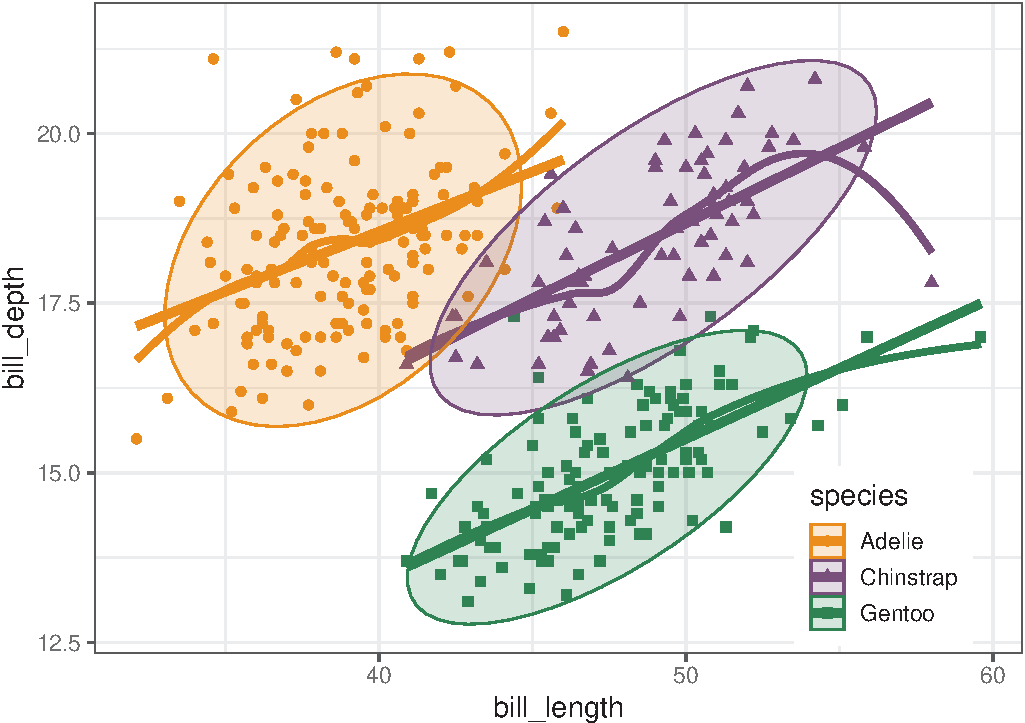
\includegraphics[width=0.8\textwidth,height=\textheight]{figs/ch03/fig-peng-ggplot1-1.pdf}

}

\caption{\label{fig-peng-ggplot1}Penguin bill length and bill depth
according to species.}

\end{figure}

Overall, the three species occupy different regions of this 2D space and
for each species the relation between bill length and depth appears
reasonably linear. Given this, we can suppress plotting the data points
to get a visual summary of the data using the fitted regression lines
and data ellipses, as shown in Figure~\ref{fig-peng-ggplot2}.

This idea, of \textbf{visual thinning} a graph to focus on what should
be seen, becomes increasingly useful as the data becomes more complex.
The \texttt{ggplot2} framework encourages this, because we can think of
various components as layers, to be included or not. Here I chose to
include only the regression line and add data ellipses of 40\%, 68\% and
95\% coverage to highlight the increasing bivariate density around the
group means.

\begin{Shaded}
\begin{Highlighting}[]
\FunctionTok{ggplot}\NormalTok{(peng, }
       \FunctionTok{aes}\NormalTok{(}\AttributeTok{x =}\NormalTok{ bill\_length, }\AttributeTok{y =}\NormalTok{ bill\_depth,}
           \AttributeTok{color =}\NormalTok{ species, }\AttributeTok{shape =}\NormalTok{ species, }\AttributeTok{fill=}\NormalTok{species)) }\SpecialCharTok{+}
  \FunctionTok{geom\_smooth}\NormalTok{(}\AttributeTok{method =} \StringTok{"lm"}\NormalTok{,  }\AttributeTok{se=}\ConstantTok{FALSE}\NormalTok{, }\AttributeTok{linewidth=}\DecValTok{2}\NormalTok{) }\SpecialCharTok{+}
  \FunctionTok{stat\_ellipse}\NormalTok{(}\AttributeTok{geom =} \StringTok{"polygon"}\NormalTok{, }\AttributeTok{level =} \FloatTok{0.95}\NormalTok{, }\AttributeTok{alpha =} \FloatTok{0.2}\NormalTok{) }\SpecialCharTok{+}
  \FunctionTok{stat\_ellipse}\NormalTok{(}\AttributeTok{geom =} \StringTok{"polygon"}\NormalTok{, }\AttributeTok{level =} \FloatTok{0.68}\NormalTok{, }\AttributeTok{alpha =} \FloatTok{0.2}\NormalTok{) }\SpecialCharTok{+}
  \FunctionTok{stat\_ellipse}\NormalTok{(}\AttributeTok{geom =} \StringTok{"polygon"}\NormalTok{, }\AttributeTok{level =} \FloatTok{0.40}\NormalTok{, }\AttributeTok{alpha =} \FloatTok{0.2}\NormalTok{) }\SpecialCharTok{+}
  \FunctionTok{theme\_penguins}\NormalTok{(}\StringTok{"dark"}\NormalTok{) }\SpecialCharTok{+}
  \FunctionTok{theme}\NormalTok{(}\AttributeTok{legend.position =} \FunctionTok{c}\NormalTok{(}\FloatTok{0.85}\NormalTok{, }\FloatTok{0.15}\NormalTok{))}
\end{Highlighting}
\end{Shaded}

\begin{figure}[H]

{\centering 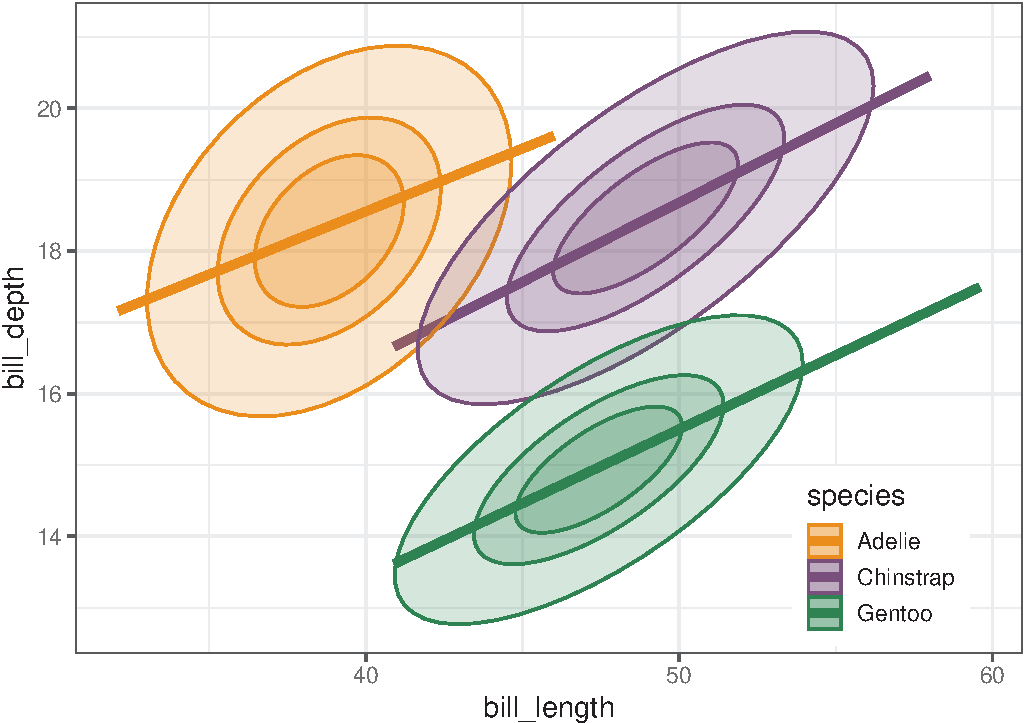
\includegraphics[width=0.8\textwidth,height=\textheight]{figs/ch03/fig-peng-ggplot2-1.pdf}

}

\caption{\label{fig-peng-ggplot2}\textbf{Visual thinning}: Suppressing
the data points gives a visual summary of the relation between bill
length and bill depth using the regression line and data ellipses.}

\end{figure}

\hypertarget{nonparamtric-bivariate-density-plots}{%
\subsubsection{Nonparamtric bivariate density
plots}\label{nonparamtric-bivariate-density-plots}}

While I emphasize data ellipses (because I like their beautiful
geometry), other visual summaries of the bivariate density are possible
and often useful.

For a single variable, \texttt{stats::density()} and
\texttt{ggplot2::geom\_density()} calculate a smoothed estimate of the
density using nonparametric kernel methods
(\protect\hyperlink{ref-Silverman:86}{Silverman, 1986}) whose smoothness
is controlled by a bandwidth parameter, analogous to the span in a loess
smoother. This idea extends to two (and more) variables
(\protect\hyperlink{ref-Scott1992}{Scott, 1992}). For bivariate data,
\texttt{MASS::kde2d()} estimates the density on a square \(n \times n\)
grid over the ranges of the variables.

\texttt{ggplot2} provides \texttt{geom\_density\_2d()} which uses
\texttt{MASS::kde2d()} and displays these as contours--- horizontal
slices of the 3D surface at equally-spaced heights and projects these
onto the 2D plane. The \textbf{ggdensity} package
(\protect\hyperlink{ref-R-ggdensity}{Otto \& Kahle, 2023}) extends this
with \texttt{geom\_hdr()}, computing the high density regions that bound
given levels of probability and maps these to the \texttt{alpha}
transparency aesthetic. A \texttt{method} argument allows you to specify
various nonparametric (\texttt{method\ ="kde"} is the default) and
parametric (\texttt{method\ ="mvnorm"} gives normal data ellipses) ways
to estimate the underlying bivariate distribution.

Figure~\ref{fig-peng-ggdensity} shows these side-by-side for comparison.
With \texttt{geom\_density\_2d()} you can specify either the number of
contour \texttt{bins} or the width of these bins (\texttt{binwidth}).
For \texttt{geom\_hdr()}, the \texttt{probs} argument gives a result
that is easier to understand.

\begin{Shaded}
\begin{Highlighting}[]
\FunctionTok{library}\NormalTok{(ggdensity)}
\FunctionTok{library}\NormalTok{(patchwork)}
\NormalTok{p1 }\OtherTok{\textless{}{-}} \FunctionTok{ggplot}\NormalTok{(peng, }
       \FunctionTok{aes}\NormalTok{(}\AttributeTok{x =}\NormalTok{ bill\_length, }\AttributeTok{y =}\NormalTok{ bill\_depth,}
           \AttributeTok{color =}\NormalTok{ species)) }\SpecialCharTok{+}
  \FunctionTok{geom\_smooth}\NormalTok{(}\AttributeTok{method =} \StringTok{"lm"}\NormalTok{,  }\AttributeTok{se=}\ConstantTok{FALSE}\NormalTok{, }\AttributeTok{linewidth=}\DecValTok{2}\NormalTok{) }\SpecialCharTok{+}
  \FunctionTok{geom\_density\_2d}\NormalTok{(}\AttributeTok{linewidth =} \FloatTok{1.1}\NormalTok{, }\AttributeTok{bins =} \DecValTok{8}\NormalTok{) }\SpecialCharTok{+}
  \FunctionTok{ggtitle}\NormalTok{(}\StringTok{"geom\_density\_2d"}\NormalTok{) }\SpecialCharTok{+}
  \FunctionTok{theme\_bw}\NormalTok{(}\AttributeTok{base\_size =} \DecValTok{14}\NormalTok{) }\SpecialCharTok{+} 
  \FunctionTok{theme\_penguins}\NormalTok{() }\SpecialCharTok{+}
  \FunctionTok{theme}\NormalTok{(}\AttributeTok{legend.position =} \FunctionTok{c}\NormalTok{(}\FloatTok{0.85}\NormalTok{, }\FloatTok{0.15}\NormalTok{))}

\NormalTok{p2 }\OtherTok{\textless{}{-}} \FunctionTok{ggplot}\NormalTok{(peng, }
       \FunctionTok{aes}\NormalTok{(}\AttributeTok{x =}\NormalTok{ bill\_length, }\AttributeTok{y =}\NormalTok{ bill\_depth,}
           \AttributeTok{color =}\NormalTok{ species, }\AttributeTok{fill =}\NormalTok{ species)) }\SpecialCharTok{+}
  \FunctionTok{geom\_smooth}\NormalTok{(}\AttributeTok{method =} \StringTok{"lm"}\NormalTok{,  }\AttributeTok{se=}\ConstantTok{FALSE}\NormalTok{, }\AttributeTok{linewidth=}\DecValTok{2}\NormalTok{) }\SpecialCharTok{+}
  \FunctionTok{geom\_hdr}\NormalTok{(}\AttributeTok{probs =} \FunctionTok{c}\NormalTok{(}\FloatTok{0.95}\NormalTok{, }\FloatTok{0.68}\NormalTok{, }\FloatTok{0.4}\NormalTok{), }\AttributeTok{show.legend =} \ConstantTok{FALSE}\NormalTok{) }\SpecialCharTok{+}
  \FunctionTok{ggtitle}\NormalTok{(}\StringTok{"ggdensity::geom\_hdr"}\NormalTok{) }\SpecialCharTok{+}
  \FunctionTok{theme\_bw}\NormalTok{(}\AttributeTok{base\_size =} \DecValTok{14}\NormalTok{) }\SpecialCharTok{+}
  \FunctionTok{theme\_penguins}\NormalTok{() }\SpecialCharTok{+}
  \FunctionTok{theme}\NormalTok{(}\AttributeTok{legend.position =} \StringTok{"none"}\NormalTok{)}

\NormalTok{p1 }\SpecialCharTok{+}\NormalTok{ p2}
\end{Highlighting}
\end{Shaded}

\begin{figure}[H]

{\centering 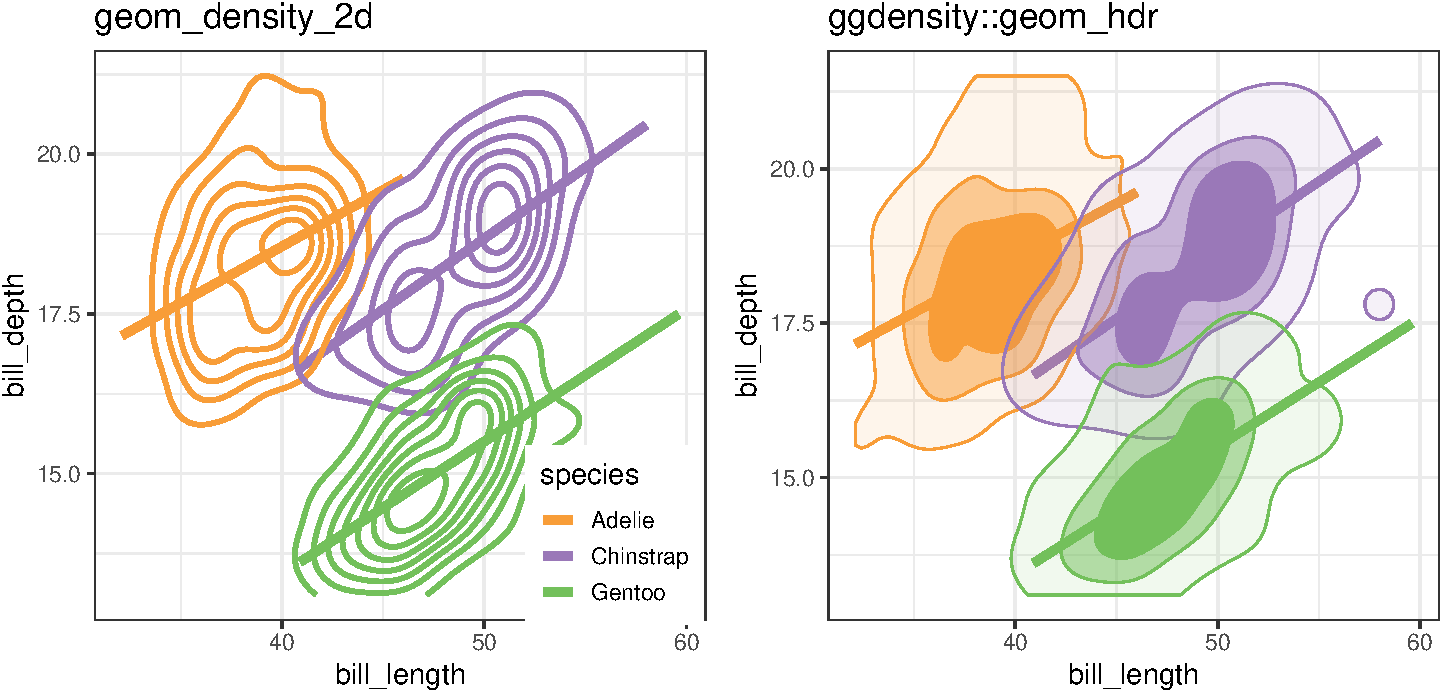
\includegraphics[width=1.2\textwidth,height=\textheight]{figs/ch03/fig-peng-ggdensity-1.pdf}

}

\caption{\label{fig-peng-ggdensity}\textbf{Bivariate densities} show the
contours of the 3D surface representing the frequency in the joint
distribution of bill length and bill depth.}

\end{figure}

\hypertarget{sec-scatmat}{%
\section{Scatterplot matrices}\label{sec-scatmat}}

Going beyond bivariate scatterplots, a \emph{pairs} plot (or
\emph{scatterplot matrix}) displays all possible \(p \times p\) pairs of
\(p\) variables in a matrix-like display where variables \((x_i, x_j)\)
are shown in a plot for row \(i\), column \(j\). This idea, due to
Hartigan (\protect\hyperlink{ref-Hartigan:75b}{1975b}), uses small
multiple plots, so that the eye can easily scan across a row or down a
column to see how a given variable is related to all the others.

The most basic version is provided by \texttt{pairs()} in base R. When
one variable is considered as an outcome or response, it is usually
helpful to put this in the first row and column. For the
\texttt{Prestige} data, in addition to income and education, we also
have a measure of \% women in each occupational category.

Plotting these together gives Figure~\ref{fig-prestige-pairs}. In such
plots, the diagonal cells give labels for the variables, but they are
also a guide to interpreting what is shown. In each row, say row 2 for
\texttt{income}, income is the vertical \(y\) variable in plots against
other variables. In each column, say column 3 for \texttt{education},
education is the horizontal \(x\) variable.

\begin{Shaded}
\begin{Highlighting}[]
\FunctionTok{pairs}\NormalTok{(}\SpecialCharTok{\textasciitilde{}}\NormalTok{ prestige }\SpecialCharTok{+}\NormalTok{ income }\SpecialCharTok{+}\NormalTok{ education }\SpecialCharTok{+}\NormalTok{ women,}
      \AttributeTok{data=}\NormalTok{Prestige)}
\end{Highlighting}
\end{Shaded}

\begin{figure}[H]

{\centering 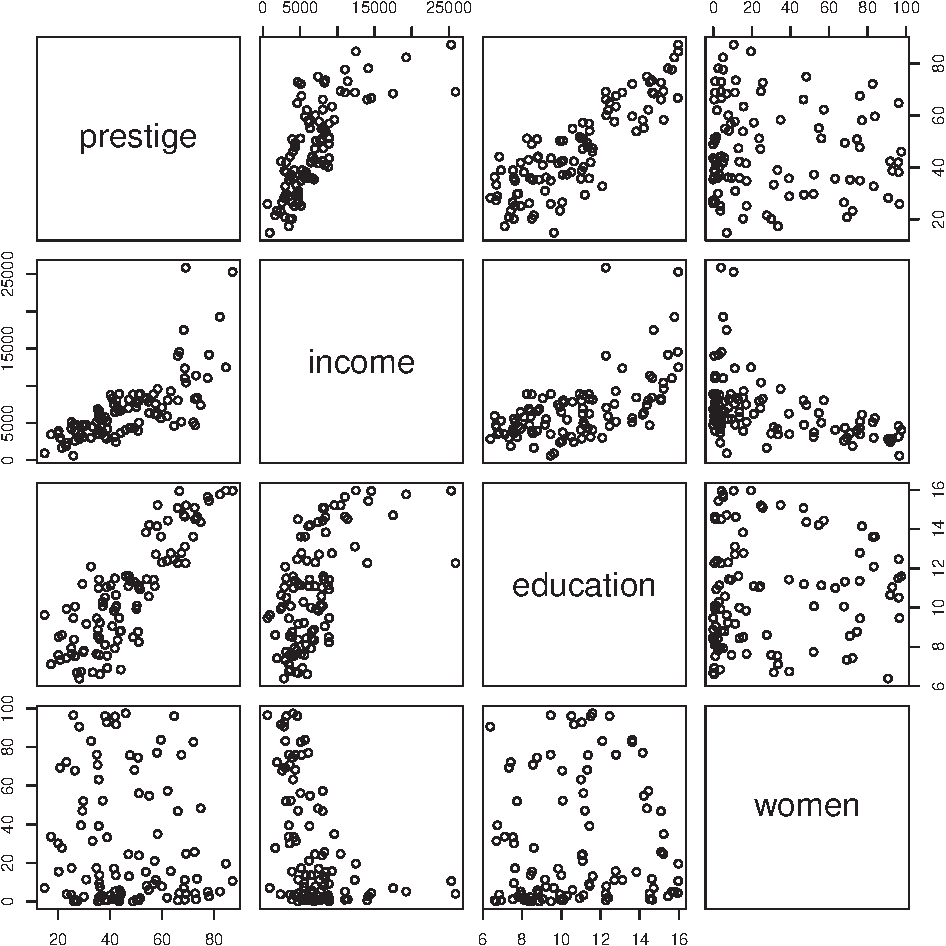
\includegraphics[width=1\textwidth,height=\textheight]{figs/ch03/fig-prestige-pairs-1.pdf}

}

\caption{\label{fig-prestige-pairs}Scatterplot matrix of the variables
in the Prestige dataset produced by \texttt{pairs()}}

\end{figure}

The plots in the first row show what we have seen before for the
relations between prestige and income and education, adding to those the
plot of prestige vs.~\% women. Plots in the first column show the same
data, but with \(x\) and \(y\) interchanged.

But this basic \texttt{pairs()} plot is very limited. A more
feature-rich version is provided by \texttt{car::scatterplotMatrix()}
which can add the regression lines, loess smooths and data ellipses for
each pair, as shown in Figure~\ref{fig-prestige-spm1}.

The diagonal panels show density curves for the distribution of each
variable; for example, the distribution of \texttt{education} appears to
be multi-modal and that of \texttt{women} shows that most of the
occupations have a low percentage of women.

The combination of the regression line with the loess smoothed curve,
but without their confidence envelopes, provides about the right amount
of detail to take in at a glance where the relations are non-linear.
We've already seen (Figure~\ref{fig-Prestige-scatterplot-income1}) the
non-linear relation between prestige and income (row 1, column 2) when
occupational type is ignored. But all relations with income in column 2
are non-linear, reinforcing our idea (Section~\ref{sec-log-scale}) that
effects of income should be assessed on a log scale.

\begin{Shaded}
\begin{Highlighting}[]
\FunctionTok{scatterplotMatrix}\NormalTok{(}\SpecialCharTok{\textasciitilde{}}\NormalTok{ prestige }\SpecialCharTok{+}\NormalTok{ income }\SpecialCharTok{+}\NormalTok{ education }\SpecialCharTok{+}\NormalTok{ women,}
  \AttributeTok{data=}\NormalTok{Prestige,}
  \AttributeTok{regLine =} \FunctionTok{list}\NormalTok{(}\AttributeTok{method=}\NormalTok{lm, }\AttributeTok{lty=}\DecValTok{1}\NormalTok{, }\AttributeTok{lwd=}\DecValTok{2}\NormalTok{, }\AttributeTok{col=}\StringTok{"black"}\NormalTok{),}
  \AttributeTok{smooth=}\FunctionTok{list}\NormalTok{(}\AttributeTok{smoother=}\NormalTok{loessLine, }\AttributeTok{spread=}\ConstantTok{FALSE}\NormalTok{,}
              \AttributeTok{lty.smooth=}\DecValTok{1}\NormalTok{, }\AttributeTok{lwd.smooth=}\DecValTok{3}\NormalTok{, }\AttributeTok{col.smooth=}\StringTok{"red"}\NormalTok{),}
  \AttributeTok{ellipse=}\FunctionTok{list}\NormalTok{(}\AttributeTok{levels=}\FloatTok{0.68}\NormalTok{, }\AttributeTok{fill.alpha=}\FloatTok{0.1}\NormalTok{))}
\end{Highlighting}
\end{Shaded}

\begin{figure}[H]

{\centering 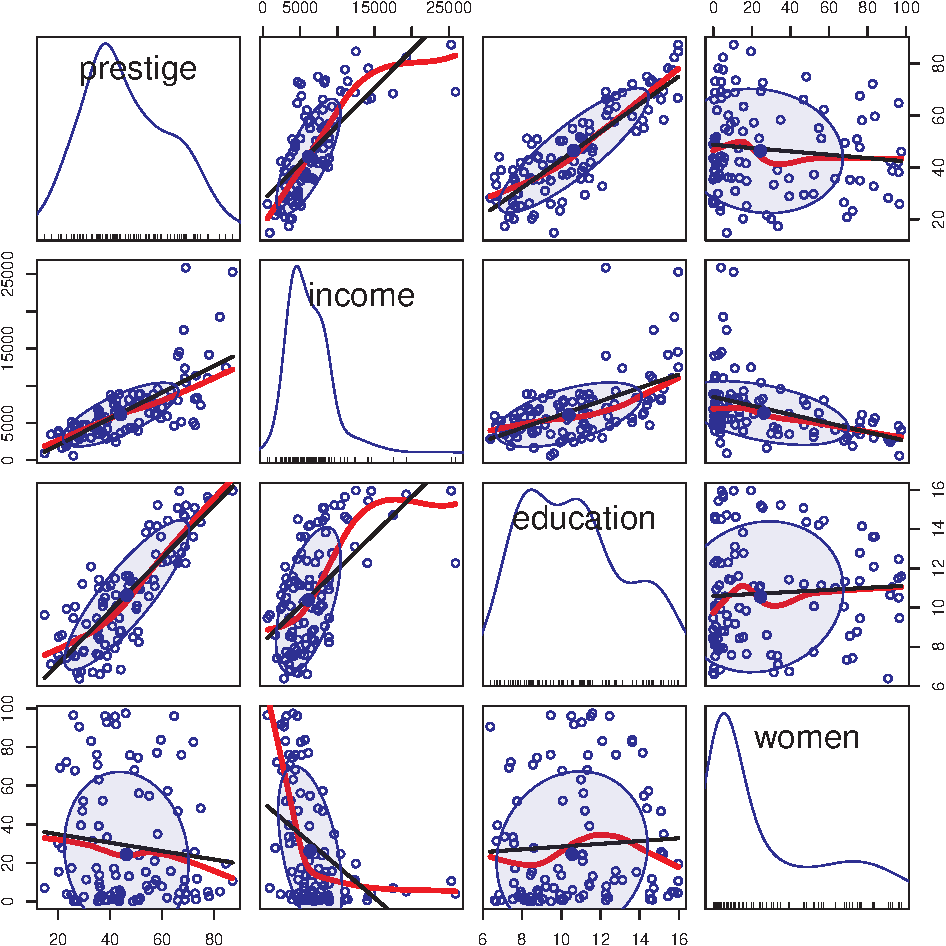
\includegraphics[width=1\textwidth,height=\textheight]{figs/ch03/fig-prestige-spm1-1.pdf}

}

\caption{\label{fig-prestige-spm1}Scatterplot matrix of the variables in
the Prestige dataset from \texttt{car::scatterplotMatrix()}.}

\end{figure}

\texttt{scatterplotMatrix()} can also label points using the
\texttt{id\ =} argument (though this can get messy) and can stratify the
observations by a grouping variable with different symbols and colors.
For example, Figure~\ref{fig-prestige-spm2} uses the syntax
\texttt{\textasciitilde{}\ prestige\ +\ education\ +\ income\ +\ women\ \textbar{}\ type}
to provide separate regression lines, smoothed curves and data ellipses
for the three types of occupations. (The default colors are somewhat
garish, so I use \texttt{scales::hue\_pal()} to mimic the discrete color
scale used in \texttt{ggplot2}).

\begin{Shaded}
\begin{Highlighting}[]
\FunctionTok{scatterplotMatrix}\NormalTok{(}\SpecialCharTok{\textasciitilde{}}\NormalTok{ prestige }\SpecialCharTok{+}\NormalTok{ income }\SpecialCharTok{+}\NormalTok{ education }\SpecialCharTok{+}\NormalTok{ women }\SpecialCharTok{|}\NormalTok{ type,}
  \AttributeTok{data =}\NormalTok{ Prestige,}
  \AttributeTok{col =}\NormalTok{ scales}\SpecialCharTok{::}\FunctionTok{hue\_pal}\NormalTok{()(}\DecValTok{3}\NormalTok{),}
  \AttributeTok{pch =} \DecValTok{15}\SpecialCharTok{:}\DecValTok{17}\NormalTok{,}
  \AttributeTok{smooth=}\FunctionTok{list}\NormalTok{(}\AttributeTok{smoother=}\NormalTok{loessLine, }\AttributeTok{spread=}\ConstantTok{FALSE}\NormalTok{,}
              \AttributeTok{lty.smooth=}\DecValTok{1}\NormalTok{, }\AttributeTok{lwd.smooth=}\DecValTok{3}\NormalTok{, }\AttributeTok{col.smooth=}\StringTok{"black"}\NormalTok{),}
  \AttributeTok{ellipse=}\FunctionTok{list}\NormalTok{(}\AttributeTok{levels=}\FloatTok{0.68}\NormalTok{, }\AttributeTok{fill.alpha=}\FloatTok{0.1}\NormalTok{))}
\end{Highlighting}
\end{Shaded}

\begin{figure}[H]

{\centering 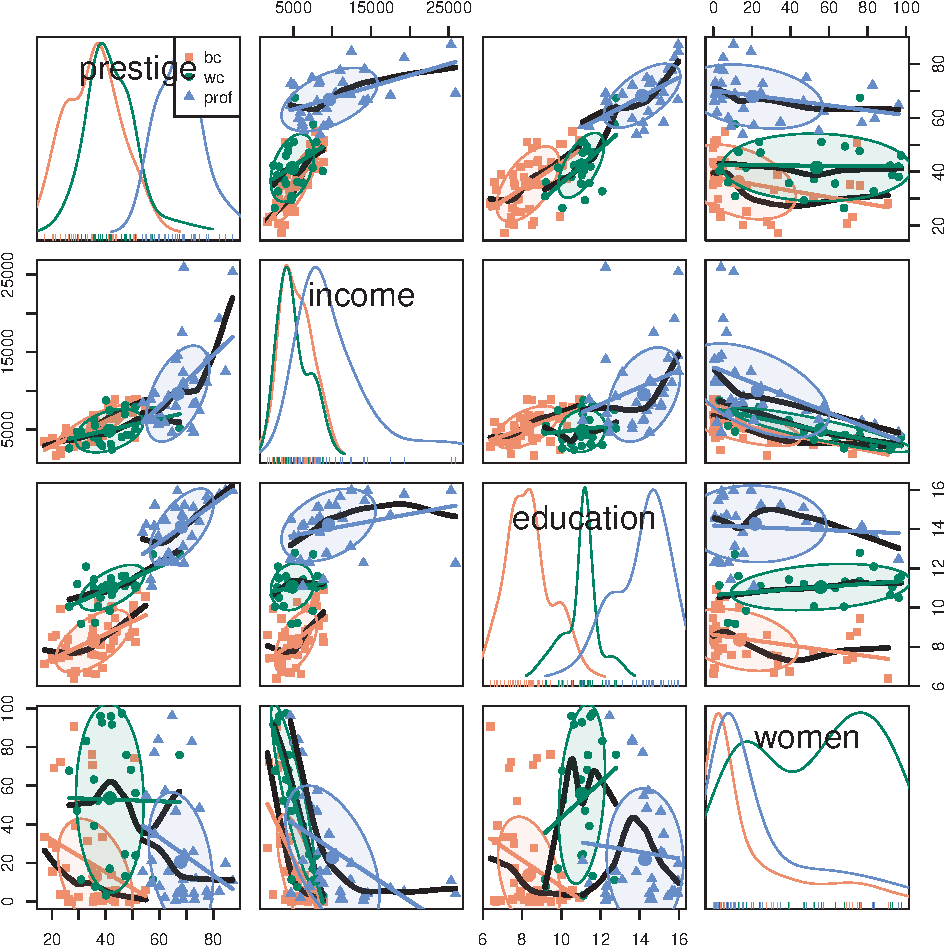
\includegraphics[width=1\textwidth,height=\textheight]{figs/ch03/fig-prestige-spm2-1.pdf}

}

\caption{\label{fig-prestige-spm2}Scatterplot matrix of the variables in
the Prestige dataset from \texttt{car::scatterplotMatrix()}, stratified
by type of occupation.}

\end{figure}

It is now easy to see why education is multi-modal: blue collar, white
collar and professional occupations have largely non-overlapping years
of education. As well, the distribution of \% women is much higher in
the white collar category.

For the \texttt{penguins} data, given what we've seen before in
Figure~\ref{fig-peng-ggplot1} and Figure~\ref{fig-peng-ggplot2}, we may
wish to suppress details of the points (\texttt{plot.points\ =\ FALSE})
and loess smooths (\texttt{smooth\ =\ FALSE}) to focus attention on the
similarity of regression lines and data ellipses for the three penguin
species. In Figure~\ref{fig-peng-spm}, I've chosen to show boxplots
rather than density curves in the diagonal panels in order to highlight
differences in the means and interquartile ranges of the species, and to
show 68\% and 95\% data ellipses in the off-diagonal panels.

\begin{Shaded}
\begin{Highlighting}[]
\FunctionTok{scatterplotMatrix}\NormalTok{(}\SpecialCharTok{\textasciitilde{}}\NormalTok{ bill\_length }\SpecialCharTok{+}\NormalTok{ bill\_depth }\SpecialCharTok{+}\NormalTok{ flipper\_length }\SpecialCharTok{+}\NormalTok{ body\_mass }\SpecialCharTok{|}\NormalTok{ species,}
  \AttributeTok{data =}\NormalTok{ peng, }
  \AttributeTok{col =} \FunctionTok{peng.colors}\NormalTok{(}\StringTok{"medium"}\NormalTok{), }
  \AttributeTok{legend=}\ConstantTok{FALSE}\NormalTok{,}
  \AttributeTok{ellipse =} \FunctionTok{list}\NormalTok{(}\AttributeTok{levels =} \FunctionTok{c}\NormalTok{(}\FloatTok{0.68}\NormalTok{, }\FloatTok{0.95}\NormalTok{), }
                 \AttributeTok{fill.alpha =} \FloatTok{0.1}\NormalTok{),}
  \AttributeTok{regLine =} \FunctionTok{list}\NormalTok{(}\AttributeTok{lwd=}\DecValTok{3}\NormalTok{),}
  \AttributeTok{diagonal =} \FunctionTok{list}\NormalTok{(}\AttributeTok{method =} \StringTok{"boxplot"}\NormalTok{),}
  \AttributeTok{smooth =} \ConstantTok{FALSE}\NormalTok{,}
  \AttributeTok{plot.points =} \ConstantTok{FALSE}\NormalTok{,}
  \AttributeTok{cex.labels=}\DecValTok{1}\NormalTok{) }
\end{Highlighting}
\end{Shaded}

\begin{figure}[H]

{\centering 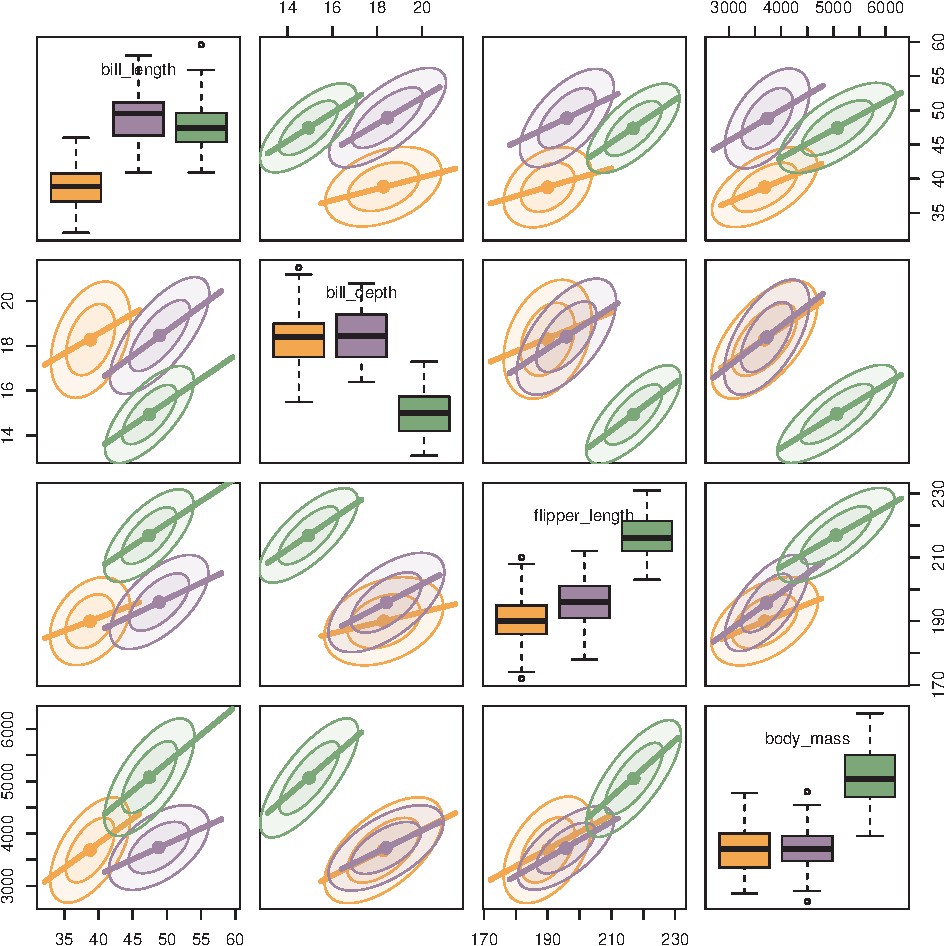
\includegraphics[width=1\textwidth,height=\textheight]{figs/ch03/fig-peng-spm-1.pdf}

}

\caption{\label{fig-peng-spm}Scatterplot matrix of the variables in the
penguins dataset, stratified by species.}

\end{figure}

It can be seen that the species are widely separated in most of the
bivariate plots. As well, the regression lines for species have similar
slopes and the data ellipses have similar size and shape in most of the
plots. From the boxplots, we can also see that
\textcolor{orange}{Adelie} penguins have shorter bill lengths than the
others, while \textcolor{green}{Gentoo} penguins have smaller bill
depth, but longer flippers and are heavier than
\textcolor{purple}{Chinstrap} and \textcolor{orange}{Adelie} penguins.

\begin{tcolorbox}[enhanced jigsaw, colback=white, rightrule=.15mm, left=2mm, arc=.35mm, colframe=quarto-callout-note-color-frame, toptitle=1mm, breakable, leftrule=.75mm, opacityback=0, bottomtitle=1mm, colbacktitle=quarto-callout-note-color!10!white, opacitybacktitle=0.6, titlerule=0mm, toprule=.15mm, title=\textcolor{quarto-callout-note-color}{\faInfo}\hspace{0.5em}{Looking ahead}, bottomrule=.15mm, coltitle=black]

Figure~\ref{fig-peng-spm} provides a reasonably complete visual summary
of the data in relation to multivariate models that ask ``do the species
differ in their means on these body size measures?'' This corresponds to
the MANOVA model,

\begin{Shaded}
\begin{Highlighting}[]
\NormalTok{peng.mod }\OtherTok{\textless{}{-}} \FunctionTok{lm}\NormalTok{(}\FunctionTok{cbind}\NormalTok{(bill\_length, bill\_depth, flipper\_length, body\_mass) }\SpecialCharTok{\textasciitilde{}}\NormalTok{ species, }
               \AttributeTok{data=}\NormalTok{peng)}
\end{Highlighting}
\end{Shaded}

Hypothesis-error (HE) plots, described in Chapter~\ref{sec-vis-mlm}
provide a better summary of the evidence for the MANOVA test of
differences among means on all variables together. These give an
\(\mathbf{H}\) ellipse reflecting the differences among means, to be
compared with an \(\mathbf{E}\) ellipse reflecting within-group
variation and a visual test of significance.

A related question is ``how well are the penguin species distinguished
by these body size measures?'' Here, the relevant model is linear
discriminant analysis (LDA), where \texttt{species} plays the role of
the response in the model,

\begin{Shaded}
\begin{Highlighting}[]
\NormalTok{peng.lda }\OtherTok{\textless{}{-}}\NormalTok{ MASS}\SpecialCharTok{:}\FunctionTok{lda}\NormalTok{( species }\SpecialCharTok{\textasciitilde{}} \FunctionTok{cbind}\NormalTok{(bill\_length, bill\_depth, flipper\_length, body\_mass), }
               \AttributeTok{data=}\NormalTok{peng)}
\end{Highlighting}
\end{Shaded}

Both MANOVA and LDA depend on the assumption that the variances and
correlations between the variables are the same for all groups. This
assumption can be tested and visualized using the methods in
Chapter~\ref{sec-eqcov}.

\end{tcolorbox}

\hypertarget{visual-thinning}{%
\subsection{Visual thinning}\label{visual-thinning}}

What can you do if there are even more variables than in these examples?
If what you want is a high-level, zoomed-out display summarizing the
pairwise relations more strongly, you can apply the idea of visual
thinning to show only the most important features.

This example uses data on the rate of various crimes in the 50 U.S.
states from the United States Statistical Abstracts, 1970, used by
Hartigan (\protect\hyperlink{ref-Hartigan:75}{1975a}) and Friendly
(\protect\hyperlink{ref-Friendly:91}{1991}). These are ordered in the
dataset roughly by seriousness of crime or from crimes of violence to
property crimes.

\begin{Shaded}
\begin{Highlighting}[]
\FunctionTok{data}\NormalTok{(crime, }\AttributeTok{package =} \StringTok{"ggbiplot"}\NormalTok{)}
\FunctionTok{str}\NormalTok{(crime)}
\CommentTok{\#\textgreater{} \textquotesingle{}data.frame\textquotesingle{}:    50 obs. of  10 variables:}
\CommentTok{\#\textgreater{}  $ state   : chr  "Alabama" "Alaska" "Arizona" "Arkansas" ...}
\CommentTok{\#\textgreater{}  $ murder  : num  14.2 10.8 9.5 8.8 11.5 6.3 4.2 6 10.2 11.7 ...}
\CommentTok{\#\textgreater{}  $ rape    : num  25.2 51.6 34.2 27.6 49.4 42 16.8 24.9 39.6 31.1 ...}
\CommentTok{\#\textgreater{}  $ robbery : num  96.8 96.8 138.2 83.2 287 ...}
\CommentTok{\#\textgreater{}  $ assault : num  278 284 312 203 358 ...}
\CommentTok{\#\textgreater{}  $ burglary: num  1136 1332 2346 973 2139 ...}
\CommentTok{\#\textgreater{}  $ larceny : num  1882 3370 4467 1862 3500 ...}
\CommentTok{\#\textgreater{}  $ auto    : num  281 753 440 183 664 ...}
\CommentTok{\#\textgreater{}  $ st      : chr  "AL" "AK" "AZ" "AR" ...}
\CommentTok{\#\textgreater{}  $ region  : Factor w/ 4 levels "Northeast","South",..: 2 4 4 2 4 4 1 2 2 2 ...}
\end{Highlighting}
\end{Shaded}

Figure~\ref{fig-crime-spm} displays the scatterplot matrix for these
seven variables, using only the regression line and data ellipse to show
the linear relation and the loess smooth to show potential
non-linearity. To make this even more schematic, the axis tick marks and
labels are also removed using the \texttt{par()} settings
\texttt{xaxt\ =\ "n",\ yaxt\ =\ "n"}.

\begin{Shaded}
\begin{Highlighting}[]
\NormalTok{crime }\SpecialCharTok{|\textgreater{}}
  \FunctionTok{select}\NormalTok{(}\FunctionTok{where}\NormalTok{(is.numeric)) }\SpecialCharTok{|\textgreater{}}
  \FunctionTok{scatterplotMatrix}\NormalTok{(}
    \AttributeTok{plot.points =} \ConstantTok{FALSE}\NormalTok{,}
    \AttributeTok{ellipse =} \FunctionTok{list}\NormalTok{(}\AttributeTok{levels =} \FloatTok{0.68}\NormalTok{, }\AttributeTok{fill=}\ConstantTok{FALSE}\NormalTok{),}
    \AttributeTok{smooth =} \FunctionTok{list}\NormalTok{(}\AttributeTok{spread =} \ConstantTok{FALSE}\NormalTok{, }
                  \AttributeTok{lwd.smooth=}\DecValTok{2}\NormalTok{, }\AttributeTok{lty.smooth =} \DecValTok{1}\NormalTok{, }\AttributeTok{col.smooth =} \StringTok{"red"}\NormalTok{),}
    \AttributeTok{cex.labels =} \DecValTok{2}\NormalTok{,}
    \AttributeTok{xaxt =} \StringTok{"n"}\NormalTok{, }\AttributeTok{yaxt =} \StringTok{"n"}\NormalTok{)}
\end{Highlighting}
\end{Shaded}

\begin{figure}[H]

{\centering 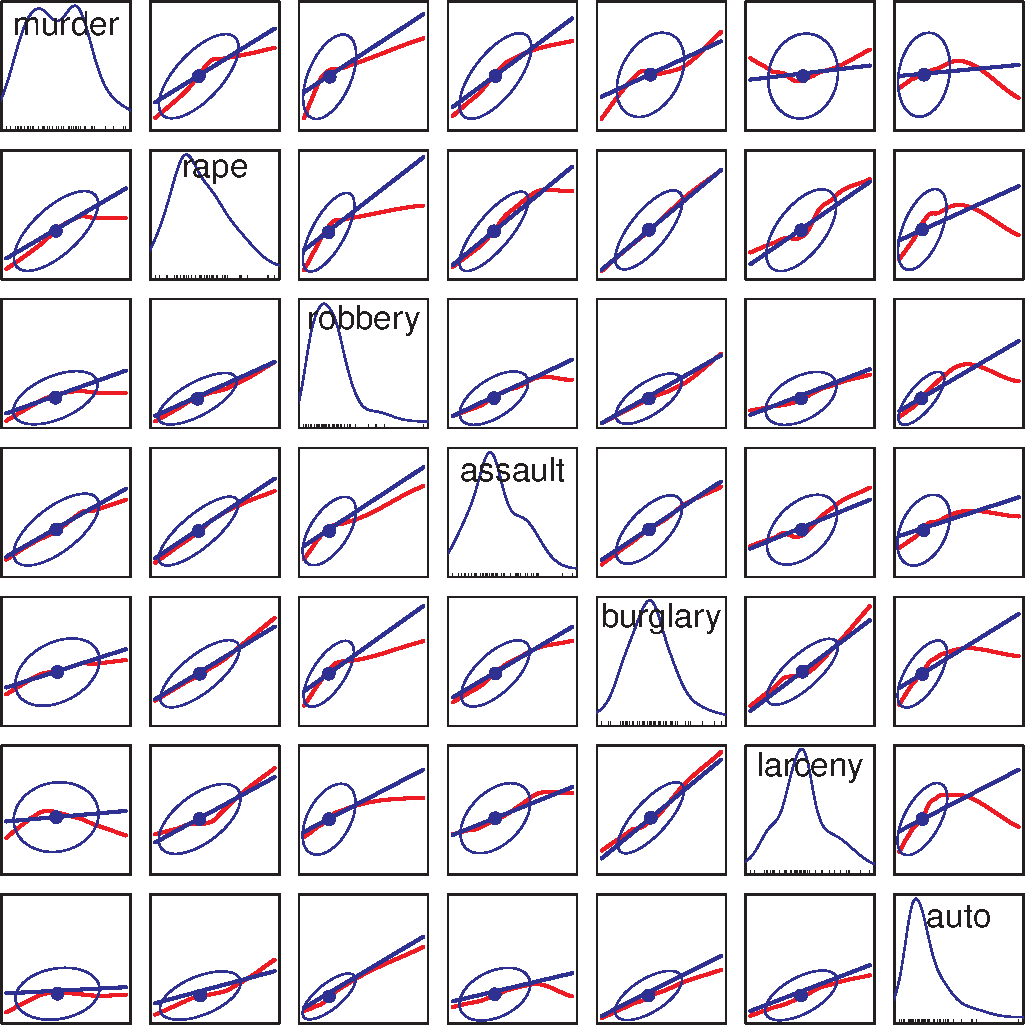
\includegraphics[width=1\textwidth,height=\textheight]{figs/ch03/fig-crime-spm-1.pdf}

}

\caption{\label{fig-crime-spm}\textbf{Visual thinning}: Scatterplot
matrix of the crime data, showing only high-level summaries of the
linear and nonlinear relations betgween each pair of variables.}

\end{figure}

We can see that all pairwise correlations are positive, pairs closer to
the main diagonal tend to be more highly correlated and in most cases
the nonparametric smooth doesn't differ much from the linear regression
line. Exceptions to this appear mainly in the columns for
\texttt{robbery} and \texttt{auto} (auto theft).

\hypertarget{sec-corrgram}{%
\subsection{Corrgrams}\label{sec-corrgram}}

What if you want to summarize the data even further, for example to show
only the value of the correlation for each pair of variables? A
\textbf{corrgram}
(\protect\hyperlink{ref-Friendly:02:corrgram}{Friendly, 2002}) is a
visual display of a correlation matrix, where the correlation can be
rendered in a variety of ways to show the direction and magnitude:
circular ``pac-man'' (or pie) symbols, ellipses, colored vars or shaded
rectangles, as shown in Figure~\ref{fig-corrgram-renderings}.

Another aspect is that of \textbf{effect ordering}
(\protect\hyperlink{ref-FriendlyKwan:03:effect}{Friendly \& Kwan,
2003}), ordering the levels of factors and variables in graphic displays
to make important features most apparent. For variables, this means that
we can arrange the variables in a matrix-like display in such a way as
to make the pattern of relationships easiest to see. Methods to achieve
this include using principal components and cluster analysis to put the
most related variables together as described in
Chapter~\ref{sec-pca-biplot}.

\begin{figure}

{\centering 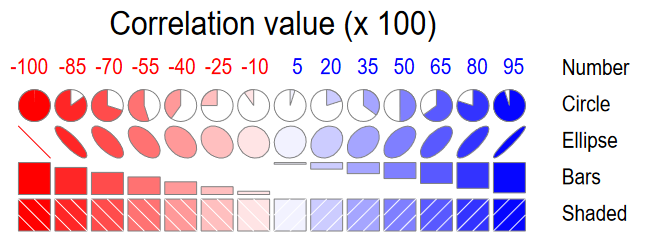
\includegraphics[width=1\textwidth,height=\textheight]{images/corrgram-renderings.png}

}

\caption{\label{fig-corrgram-renderings}\textbf{Corrgrams}: Some
renderings for the value of a correlation in a corrgram display,
conveying sign and magnitude in different ways.}

\end{figure}

In R, these diagrams can be created using the \textbf{corrgram}
(\protect\hyperlink{ref-R-corrgram}{Wright, 2021}) and \textbf{corrplot}
(\protect\hyperlink{ref-R-corrplot}{Wei \& Simko, 2021}) packages, with
different features. \texttt{corrgram::corrgram()} is closest to Friendly
(\protect\hyperlink{ref-Friendly:02:corrgram}{2002}), in that it allows
different rendering functions for the lower, upper and diagonal panels
as illustrated in Figure~\ref{fig-corrgram-renderings}. For example, a
corrgram similar to Figure~\ref{fig-crime-spm} can be produced as
follows (not shown here):

\begin{Shaded}
\begin{Highlighting}[]
\NormalTok{crime }\SpecialCharTok{|\textgreater{}}
  \FunctionTok{select}\NormalTok{(}\FunctionTok{where}\NormalTok{(is.numeric)) }\SpecialCharTok{|\textgreater{}}
  \FunctionTok{corrgram}\NormalTok{(}\AttributeTok{lower.panel =}\NormalTok{ panel.ellipse,}
           \AttributeTok{upper.panel =}\NormalTok{ panel.ellipse,}
           \AttributeTok{diag.panel =}\NormalTok{ panel.density)}
\end{Highlighting}
\end{Shaded}

\texttt{corrplot::corrplot()} provides the rendering methods
\texttt{c("circle",\ "square",\ "ellipse",\ "number",\ "shade",\ "color",\ "pie")},
but only one can be used at a time. The function
\texttt{corrplot::corrplot.mixed()} allows different options to be
selected for the lower and upper triangles. The iconic shape is colored
with a gradient in relation to the correlation value.

\begin{Shaded}
\begin{Highlighting}[]
\NormalTok{crime }\SpecialCharTok{|\textgreater{}}
  \FunctionTok{select}\NormalTok{(}\FunctionTok{where}\NormalTok{(is.numeric)) }\SpecialCharTok{|\textgreater{}}
  \FunctionTok{cor}\NormalTok{() }\SpecialCharTok{|\textgreater{}}
  \FunctionTok{corrplot.mixed}\NormalTok{(}
           \AttributeTok{lower =} \StringTok{"ellipse"}\NormalTok{,}
           \AttributeTok{upper =} \StringTok{"pie"}\NormalTok{,}
           \AttributeTok{tl.col =} \StringTok{"black"}\NormalTok{,}
           \AttributeTok{tl.srt =} \DecValTok{0}\NormalTok{,}
           \AttributeTok{addCoef.col =} \StringTok{"black"}\NormalTok{,}
           \AttributeTok{addCoefasPercent =} \ConstantTok{TRUE}\NormalTok{)}
\end{Highlighting}
\end{Shaded}

\begin{figure}[H]

{\centering 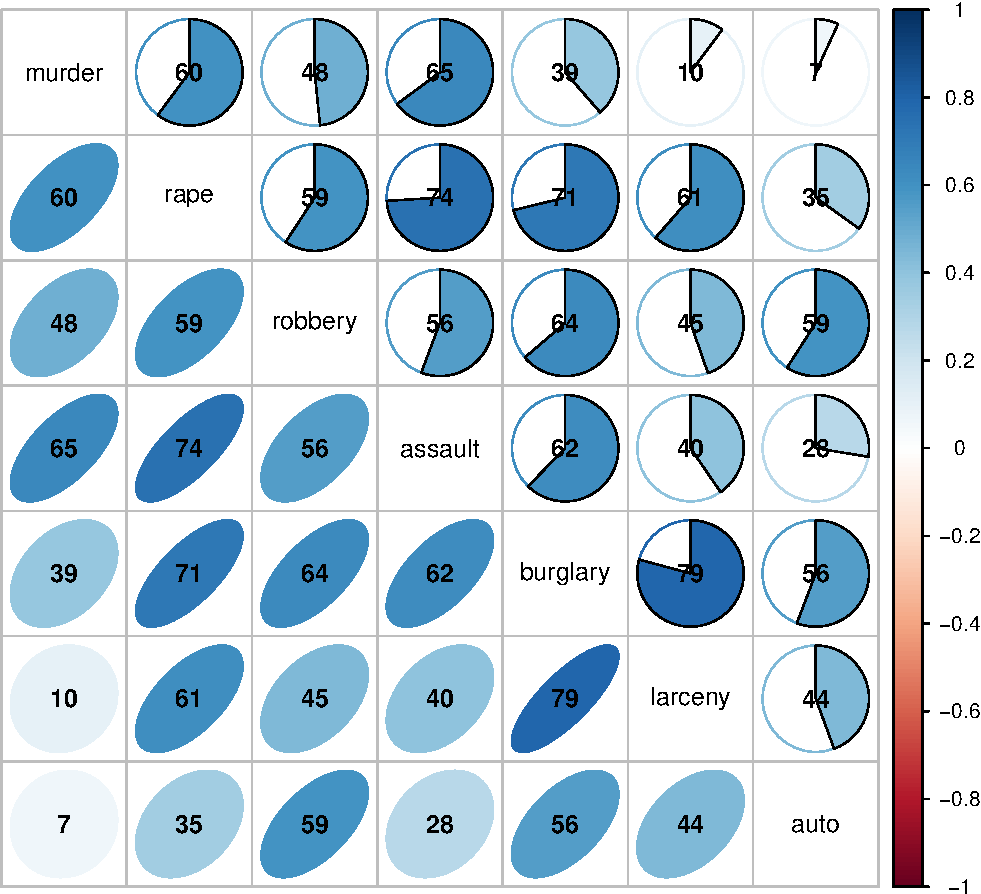
\includegraphics[width=1\textwidth,height=\textheight]{figs/ch03/fig-crime-corrplot-1.pdf}

}

\caption{\label{fig-crime-corrplot}Corrplot of the \texttt{crime} data,
showing the correlation between each pair of variables with an ellipse
(lower) and a pie chart symbol (upper), all shaded in proportion to the
correlation value, also shown numerically.}

\end{figure}

The combination of renderings shown in Figure~\ref{fig-crime-corrplot}
is instructive. Small differences among correlation values are easier to
see with the pie symbols than with the ellipses; for example, compare
the values for murder with larceny and auto theft in row 1, columns 6-7
with those in column 1, rows 6-7, where the former are easier to
distinguish. The shading color adds another visual cue.

Variations of corrgrams are worthy replacements for a numeric table of
correlations, which are often presented in publications only for
archival value. Including the numeric value (rounded here, for
presentation purposes), makes this an attractive alternative to boring
tables of correlations.

\textbf{TODO}: Add example showing correlation ordering -- e.g.,
\texttt{mtcars} data.

\hypertarget{sec-ggpairs}{%
\section{Generalized pairs plots}\label{sec-ggpairs}}

When a dataset contains one or more discrete variables, the traditional
pairs plot cannot cope, using only color and/or point symbols to
represent categorical variables. In the context of mosaic displays and
loglinear models, representing \(n\)-way frequency tables by rectangular
tiles depicting cell frequencies, I
(\protect\hyperlink{ref-Friendly:94a}{Friendly, 1994}) proposed an
analog of the scatterplot matrix using mosaic plots for each pair of
variables. The \textbf{vcd} package (\protect\hyperlink{ref-R-vcd}{Meyer
et al., 2023}) implements very general \texttt{pairs()} methods for
\texttt{"table"} objects. See my book \emph{Discrete Data Analysis with
R} (\protect\hyperlink{ref-FriendlyMeyer:2016:DDAR}{Friendly \& Meyer,
2016}) and the \textbf{vcdExtra}
(\protect\hyperlink{ref-R-vcdExtra}{Friendly, 2023}) package for mosaic
plots and mosaic matrices.

For example, we can tabulate the distributions of penguin species by sex
and the island where they were observed using \texttt{xtabs()}.
\texttt{ftable()} prints this three-way table more compactly. (In this
example, and what follows in the chapter, I've changed the labels for
sex from (``f'', ``m'') to (``Female'', ``Male'')).

\begin{Shaded}
\begin{Highlighting}[]
\CommentTok{\# use better labels for sex}
\NormalTok{peng }\OtherTok{\textless{}{-}}\NormalTok{ peng }\SpecialCharTok{|\textgreater{}}
  \FunctionTok{mutate}\NormalTok{(}\AttributeTok{sex =} \FunctionTok{factor}\NormalTok{(sex, }\AttributeTok{labels =} \FunctionTok{c}\NormalTok{(}\StringTok{"Female"}\NormalTok{, }\StringTok{"Male"}\NormalTok{)))}
\NormalTok{peng.table }\OtherTok{\textless{}{-}} \FunctionTok{xtabs}\NormalTok{(}\SpecialCharTok{\textasciitilde{}}\NormalTok{ species }\SpecialCharTok{+}\NormalTok{ sex }\SpecialCharTok{+}\NormalTok{ island, }\AttributeTok{data =}\NormalTok{ peng)}

\FunctionTok{ftable}\NormalTok{(peng.table)}
\CommentTok{\#\textgreater{}                  island Biscoe Dream Torgersen}
\CommentTok{\#\textgreater{} species   sex                                 }
\CommentTok{\#\textgreater{} Adelie    Female            22    27        24}
\CommentTok{\#\textgreater{}           Male              22    28        23}
\CommentTok{\#\textgreater{} Chinstrap Female             0    34         0}
\CommentTok{\#\textgreater{}           Male               0    34         0}
\CommentTok{\#\textgreater{} Gentoo    Female            58     0         0}
\CommentTok{\#\textgreater{}           Male              61     0         0}
\end{Highlighting}
\end{Shaded}

We can see immediately that the penguin species differ by island: only
Adelie were observed on all three islands; Biscoe Island had no
Chinstraps and Dream Island had no Gentoos.

\texttt{vcd::pairs()} produces all pairwise mosaic plots, as shown in
Figure~\ref{fig-peng-mosaic}. The diagonal panels show the one-way
frequencies by width of the divided bars. Each off-diagonal panel shows
the bivariate counts, breaking down each column variable by splitting
the bars in proportion to a second variable. Consequently, the frequency
of each cell is represented by its' area. The purpose is to show the
\textbf{pattern of association} between each pair, and so, the tiles in
the mosaic are shaded according to the signed standardized residual,
\(d_{ij} = (n_{ij} - \hat{n}_{ij}) / \sqrt{\hat{n}_{ij}}\) in a simple
\(\chi^2 = \Sigma_{ij} \; d_{ij}^2\) test for association---
\textcolor{blue}{blue} where the observed frequency \(n_{ij}\) is
significantly greater than expected \(\hat{n}_{ij}\) under independence,
and \textcolor{red}{red} where it is less than expected. The tiles are
unshaded when \(| d_{ij} | < 2\).

\begin{Shaded}
\begin{Highlighting}[]
\FunctionTok{library}\NormalTok{(vcd)}
\FunctionTok{pairs}\NormalTok{(peng.table, }\AttributeTok{shade =} \ConstantTok{TRUE}\NormalTok{,}
      \AttributeTok{lower\_panel\_args =} \FunctionTok{list}\NormalTok{(}\AttributeTok{labeling =} \FunctionTok{labeling\_values}\NormalTok{()),}
      \AttributeTok{upper\_panel\_args =} \FunctionTok{list}\NormalTok{(}\AttributeTok{labeling =} \FunctionTok{labeling\_values}\NormalTok{()))}
\end{Highlighting}
\end{Shaded}

\begin{figure}[H]

{\centering 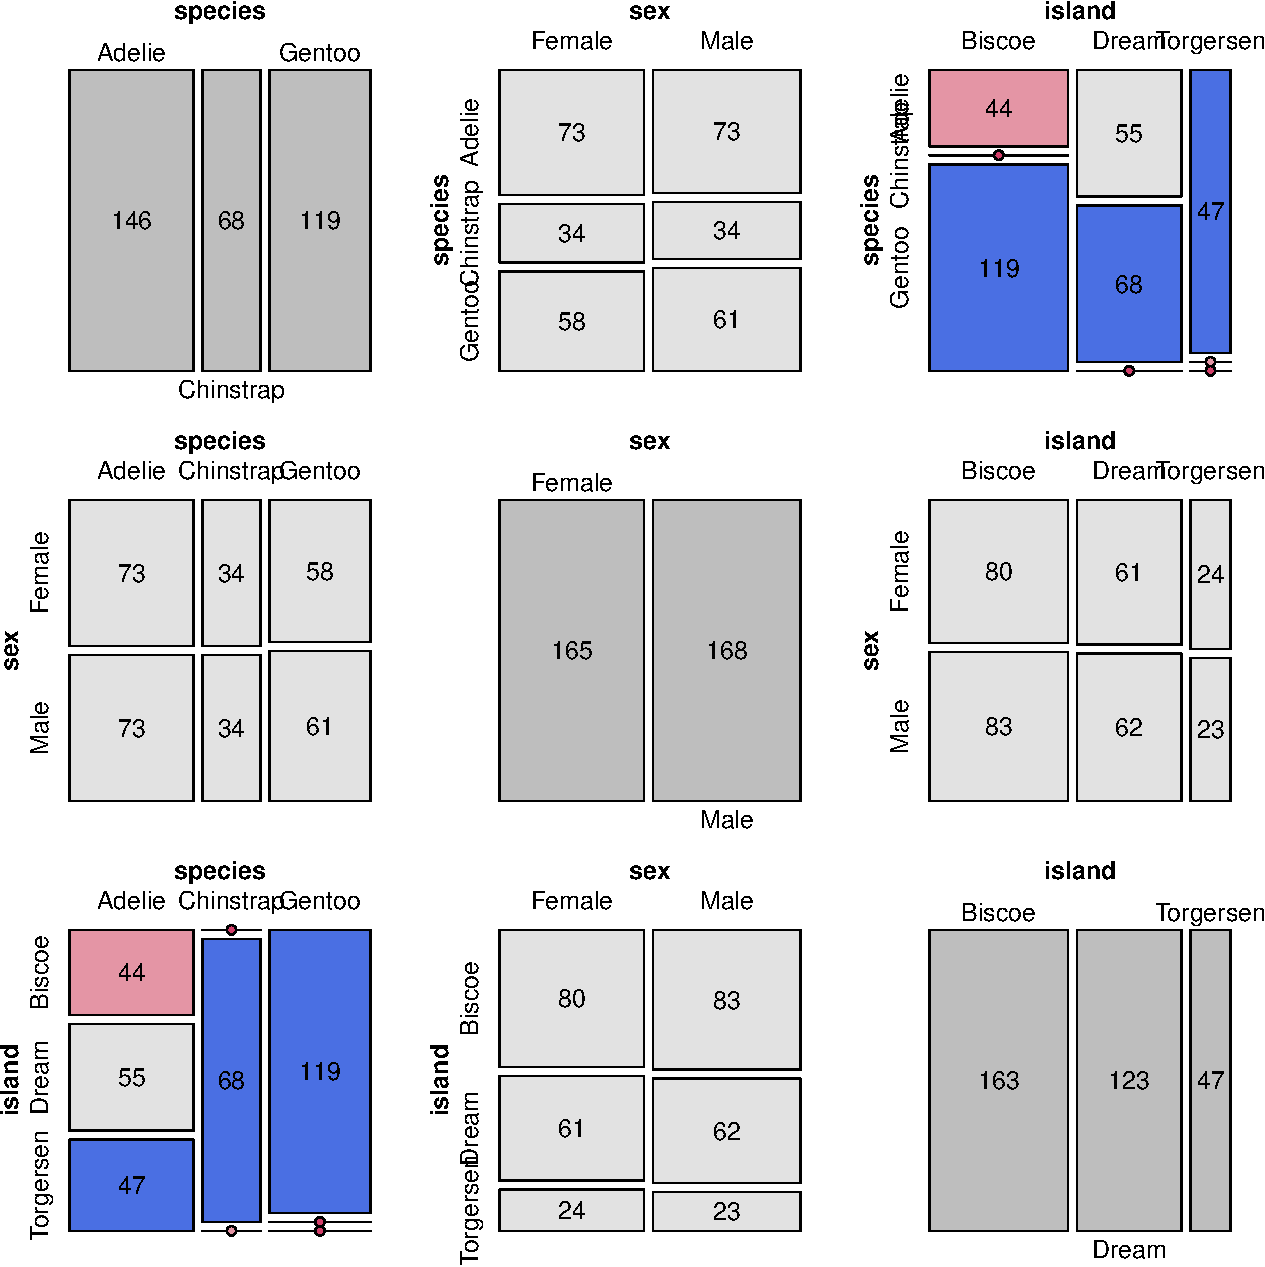
\includegraphics[width=1\textwidth,height=\textheight]{figs/ch03/fig-peng-mosaic-1.pdf}

}

\caption{\label{fig-peng-mosaic}Mosaic pairs plot for the combinations
of species, sex and island. Diagnonal plots show the marginal frequency
of each variable by the width of each rectangle. Off-diagonal mosaic
plots subdivide by the conditional frequency of the second variable,
shown numerically in the tiles.}

\end{figure}

The shading patterns in cells (1,3) and (3,1) of
Figure~\ref{fig-peng-mosaic} show what we've seen before in the table of
frequencies: The distribution of species varies across island because on
each island one or more species did not occur. Row 2 and column 2 show
that sex is nearly exactly proportional among species and islands,
indicating independence,
\(\text{sex} \perp \{\text{species}, \text{island}\}\). More
importantly, mosaic pairs plots can show, at a glance, all (bivariate)
associations among multivariate categorical variables.

The next step, by John Emerson and others
(\protect\hyperlink{ref-Emerson-etal:2013}{Emerson et al., 2013}) was to
recognize that combinations of continuous and discrete, categorical
variables could be plotted in different ways.

\begin{itemize}
\tightlist
\item
  Two continuous variables can be shown as a standard scatterplot of
  points and/or bivariate density contours, or simply by numeric
  summaries such as a correlation value;
\item
  A pair of one continuous and one categorical variable can be shown as
  side-by-side boxplots or violin plots, histograms or density plots;
\item
  Two categorical variables could be shown in a mosaic plot or by
  grouped bar plots.
\end{itemize}

In the \textbf{ggplot2} framework, these displays are implemented using
the \texttt{ggpairs()} function from the \textbf{GGally} package
(\protect\hyperlink{ref-R-GGally}{Schloerke et al., 2023}). This allows
different plot types to be shown in the lower and upper triangles and in
the diagonal cells of the plot matrix. As well, aesthetics such as color
and shape can be used within the plots to distinguish groups directly.
As illustrated below, you can define custom functions to control exactly
what is plotted in any panel.

The basic, default plot shows scatterplots for pairs of continuous
variables in the lower triangle and the values of correlations in the
upper triangle. A combination of a discrete and continuous variables is
plotted as histograms in the lower triangle and boxplots in the upper
triangle. Figure~\ref{fig-peng-ggpairs1} includes \texttt{sex} to
illustrate the combinations.

\begin{Shaded}
\begin{Highlighting}[]
\FunctionTok{ggpairs}\NormalTok{(peng, }\AttributeTok{columns=}\FunctionTok{c}\NormalTok{(}\DecValTok{3}\SpecialCharTok{:}\DecValTok{6}\NormalTok{, }\DecValTok{7}\NormalTok{),}
        \FunctionTok{aes}\NormalTok{(}\AttributeTok{color=}\NormalTok{species, }\AttributeTok{alpha=}\FloatTok{0.5}\NormalTok{),}
        \AttributeTok{progress =} \ConstantTok{FALSE}\NormalTok{) }\SpecialCharTok{+}
  \FunctionTok{theme\_penguins}\NormalTok{() }\SpecialCharTok{+}
  \FunctionTok{theme}\NormalTok{(}\AttributeTok{axis.text.x =} \FunctionTok{element\_text}\NormalTok{(}\AttributeTok{angle =} \SpecialCharTok{{-}}\DecValTok{45}\NormalTok{))}
\end{Highlighting}
\end{Shaded}

\begin{figure}[H]

{\centering 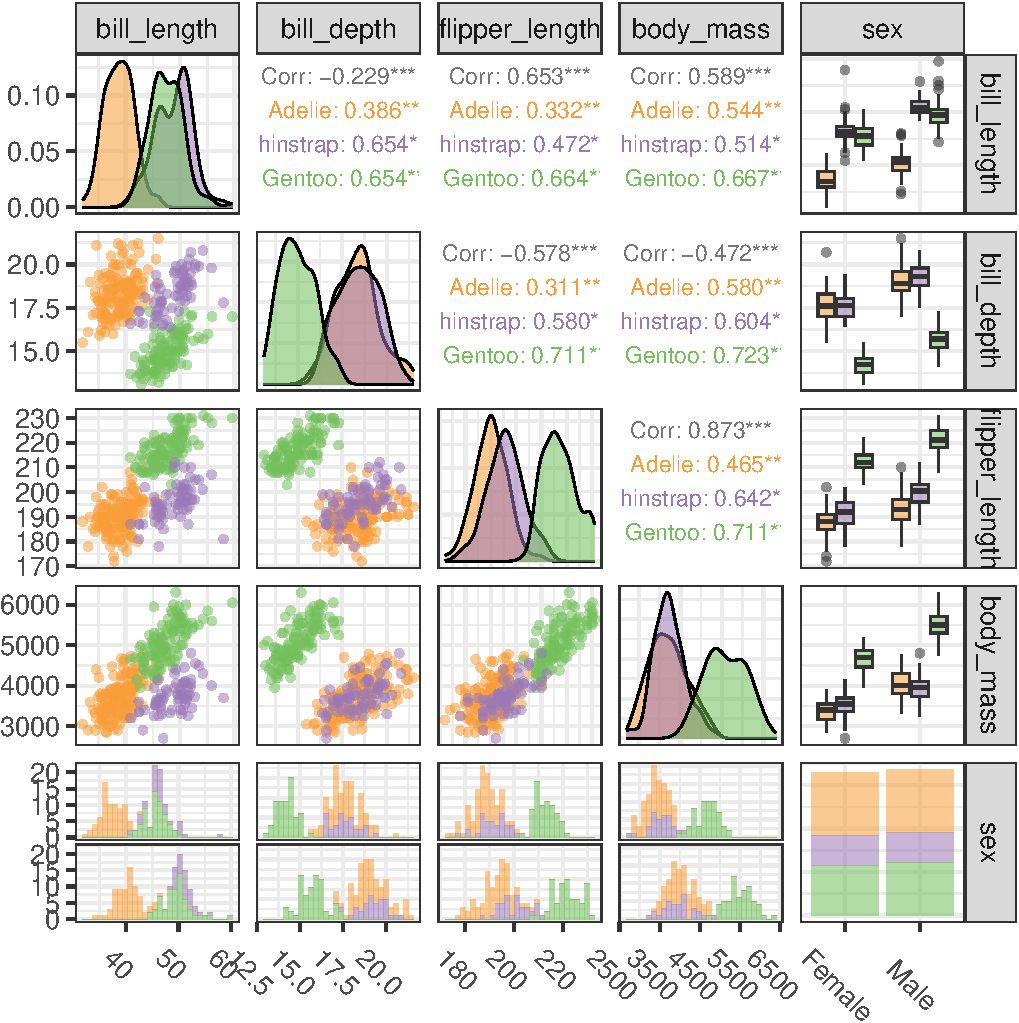
\includegraphics[width=1\textwidth,height=\textheight]{figs/ch03/fig-peng-ggpairs1-1.pdf}

}

\caption{\label{fig-peng-ggpairs1}Basic \texttt{ggpairs()} plot of
penguin size variables and sex, stratified by species.}

\end{figure}

To my eye, printing the values of correlations in the upper triangle is
often a waste of graphic space. But this example shows something
peculiar and interesting if you look closely: In all pairs among the
penguin size measurements, there are positive correlations within each
species, as we can see in Figure~\ref{fig-peng-spm}. Yet, in three of
these panels, the overall correlation ignoring species is negative. For
example, the overall correlation between bill depth and flipper length
is \(r = -0.579\) in row 2, column 3; the scatterplot in the diagonally
opposite cell, row 3, column 2 shows the data. These cases, of differing
signs for an overall correlation, ignoring a group variable and the
within group correlations are examples of \textbf{Simpson's Paradox},
explored later in Chapter XX.

The last row and column, for \texttt{sex} in
Figure~\ref{fig-peng-ggpairs1}, provides an initial glance at the issue
of sex differences among penguin species that motivated the collection
of these data. We can go further by also examining differences among
species and island, but first we need to understand how to display
exactly what we want for each pairwise plot.

\texttt{ggpairs()} is extremely general in that for each of the
\texttt{lower}, \texttt{upper} and \texttt{diag} sections you can assign
any of a large number of built-in functions (of the form
\texttt{ggally\_NAME}), or your own custom function for what is plotted,
depending on the types of variables in each plot.

\begin{itemize}
\tightlist
\item
  \texttt{continuous}: both X and Y are continuous variables, supply
  this as the \texttt{NAME} part of a \texttt{ggally\_NAME()} function
  or the name of a custom function;
\item
  \texttt{combo}: one X of and Y variable is discrete while the other is
  continuous, using the same convention;
\item
  \texttt{discrete}: both X and Y are discrete variables.
\end{itemize}

The defaults, which were used in Figure~\ref{fig-peng-ggpairs1}, are:

\begin{Shaded}
\begin{Highlighting}[]
\NormalTok{upper }\OtherTok{=} \FunctionTok{list}\NormalTok{(}\AttributeTok{continuous =} \StringTok{"cor"}\NormalTok{,          }\CommentTok{\# correlation values}
             \AttributeTok{combo =} \StringTok{"box\_no\_facet"}\NormalTok{,      }\CommentTok{\# boxplots }
             \AttributeTok{discrete =} \StringTok{"count"}\NormalTok{)          }\CommentTok{\# rectangles \textasciitilde{} count}
\NormalTok{lower }\OtherTok{=} \FunctionTok{list}\NormalTok{(}\AttributeTok{continuous =} \StringTok{"points"}\NormalTok{,       }\CommentTok{\# just data points}
             \AttributeTok{combo =} \StringTok{"facethist"}\NormalTok{,         }\CommentTok{\# faceted histograms}
             \AttributeTok{discrete =} \StringTok{"facetbar"}\NormalTok{)       }\CommentTok{\# faceted bar plots}
\NormalTok{diag  }\OtherTok{=} \FunctionTok{list}\NormalTok{(}\AttributeTok{continuous =} \StringTok{"densityDiag"}\NormalTok{,  }\CommentTok{\# density plots}
             \AttributeTok{discrete =} \StringTok{"barDiag"}\NormalTok{)        }\CommentTok{\# bar plots}
\end{Highlighting}
\end{Shaded}

Thus, \texttt{ggpairs()} uses \texttt{ggally\_cor()} to print the
correlation values for pairs of continuous variables in the upper
triangle, and uses \texttt{ggally\_points()} to plot scatterplots of
points in the lower portion. The diagonal panels as shown as density
plots (\texttt{ggally\_densityDiag()}) for continuous variables but as
bar plots (\texttt{ggally\_barDiag()}) for discrete factors.

See the vignette,
\href{https://ggobi.github.io/ggally/articles/ggally_plots.html}{ggally\_plots}
for an illustrated list of available high-level plots. For our purpose
here, which is to illustrate enhanced displays, note that for
scatterplots of continuous variables, there are two functions which plot
the points and also add a smoother, \texttt{\_lm} or \texttt{\_loess}.

\begin{Shaded}
\begin{Highlighting}[]
\FunctionTok{ls}\NormalTok{(}\FunctionTok{getNamespace}\NormalTok{(}\StringTok{"GGally"}\NormalTok{)) }\SpecialCharTok{|\textgreater{}}\NormalTok{ stringr}\SpecialCharTok{::}\FunctionTok{str\_subset}\NormalTok{(}\StringTok{"\^{}ggally\_smooth\_"}\NormalTok{)}
\CommentTok{\#\textgreater{} [1] "ggally\_smooth\_lm"    "ggally\_smooth\_loess"}
\end{Highlighting}
\end{Shaded}

A customized display for scatterplots of continuous variables can be any
function that takes \texttt{data} and \texttt{mapping} arguments and
returns a \texttt{"ggplot"} object. The \texttt{mapping} argument
supplies the aesthetics, e.g., \texttt{aes(color=species,\ alpha=0.5)},
but only if you wish to override what is supplied in the
\texttt{ggpairs()} call.

Here is a function, \texttt{my\_panel()} that plots the data points,
regression line and loess smooth:

\begin{Shaded}
\begin{Highlighting}[]
\NormalTok{my\_panel }\OtherTok{\textless{}{-}} \ControlFlowTok{function}\NormalTok{(data, mapping, ...)\{}
\NormalTok{  p }\OtherTok{\textless{}{-}} \FunctionTok{ggplot}\NormalTok{(}\AttributeTok{data =}\NormalTok{ data, }\AttributeTok{mapping =}\NormalTok{ mapping) }\SpecialCharTok{+} 
    \FunctionTok{geom\_point}\NormalTok{() }\SpecialCharTok{+} 
    \FunctionTok{geom\_smooth}\NormalTok{(}\AttributeTok{method=}\NormalTok{lm, }\AttributeTok{formula =}\NormalTok{ y }\SpecialCharTok{\textasciitilde{}}\NormalTok{ x, }\AttributeTok{se =} \ConstantTok{FALSE}\NormalTok{, ...) }\SpecialCharTok{+}
    \FunctionTok{geom\_smooth}\NormalTok{(}\AttributeTok{method=}\NormalTok{loess, }\AttributeTok{formula =}\NormalTok{ y }\SpecialCharTok{\textasciitilde{}}\NormalTok{ x, }\AttributeTok{se =} \ConstantTok{FALSE}\NormalTok{, ...)}
\NormalTok{  p}
\NormalTok{\}}
\end{Highlighting}
\end{Shaded}

For this example, I want only simple summaries of for the scatterplots,
so I don't want to plot the data points, but do want to add the
regression line and a data ellipse.

\begin{Shaded}
\begin{Highlighting}[]
\NormalTok{my\_panel1 }\OtherTok{\textless{}{-}} \ControlFlowTok{function}\NormalTok{(data, mapping, ...)\{}
\NormalTok{  p }\OtherTok{\textless{}{-}} \FunctionTok{ggplot}\NormalTok{(}\AttributeTok{data =}\NormalTok{ data, }\AttributeTok{mapping =}\NormalTok{ mapping) }\SpecialCharTok{+} 
     \FunctionTok{geom\_smooth}\NormalTok{(}\AttributeTok{method=}\NormalTok{lm, }\AttributeTok{formula =}\NormalTok{ y }\SpecialCharTok{\textasciitilde{}}\NormalTok{ x, }\AttributeTok{se =} \ConstantTok{FALSE}\NormalTok{, ...) }\SpecialCharTok{+}
     \FunctionTok{stat\_ellipse}\NormalTok{(}\AttributeTok{geom =} \StringTok{"polygon"}\NormalTok{, }\AttributeTok{level =} \FloatTok{0.68}\NormalTok{, ...)}
\NormalTok{  p}
\NormalTok{\}}
\end{Highlighting}
\end{Shaded}

Then, to show what can be done, Figure~\ref{fig-peng-ggpairs7} uses
\texttt{my\_panel1()} for the scatterplots in the 4 x 4 block of plots
in the upper left. The combination of the continuous body size measures
and the discrete factors \texttt{species}, \texttt{island} and
\texttt{sex} are shown in upper triangle by boxplots but by faceted
histograms in the lower portion. The factors are shown as rectangles
with area proportional to count (poor-man's mosaic plots) above the
diagonal and as faceted bar plots below.

\begin{Shaded}
\begin{Highlighting}[]
\FunctionTok{ggpairs}\NormalTok{(peng, }\AttributeTok{columns=}\FunctionTok{c}\NormalTok{(}\DecValTok{3}\SpecialCharTok{:}\DecValTok{6}\NormalTok{, }\DecValTok{1}\NormalTok{, }\DecValTok{2}\NormalTok{, }\DecValTok{7}\NormalTok{),}
        \AttributeTok{mapping =} \FunctionTok{aes}\NormalTok{(}\AttributeTok{color=}\NormalTok{species, }\AttributeTok{fill =}\NormalTok{ species, }\AttributeTok{alpha=}\FloatTok{0.2}\NormalTok{),}
        \AttributeTok{lower =} \FunctionTok{list}\NormalTok{(}\AttributeTok{continuous =}\NormalTok{ my\_panel1),}
        \AttributeTok{upper =} \FunctionTok{list}\NormalTok{(}\AttributeTok{continuous =}\NormalTok{ my\_panel1),}
        \AttributeTok{progress =} \ConstantTok{FALSE}\NormalTok{) }\SpecialCharTok{+}
  \FunctionTok{theme\_penguins}\NormalTok{() }\SpecialCharTok{+}
  \FunctionTok{theme}\NormalTok{(}\AttributeTok{panel.grid.major =} \FunctionTok{element\_blank}\NormalTok{(), }
        \AttributeTok{panel.grid.minor =} \FunctionTok{element\_blank}\NormalTok{()) }\SpecialCharTok{+} 
  \FunctionTok{theme}\NormalTok{(}\AttributeTok{axis.text.x =} \FunctionTok{element\_text}\NormalTok{(}\AttributeTok{angle =} \SpecialCharTok{{-}}\DecValTok{45}\NormalTok{))}
\end{Highlighting}
\end{Shaded}

\begin{figure}[H]

{\centering 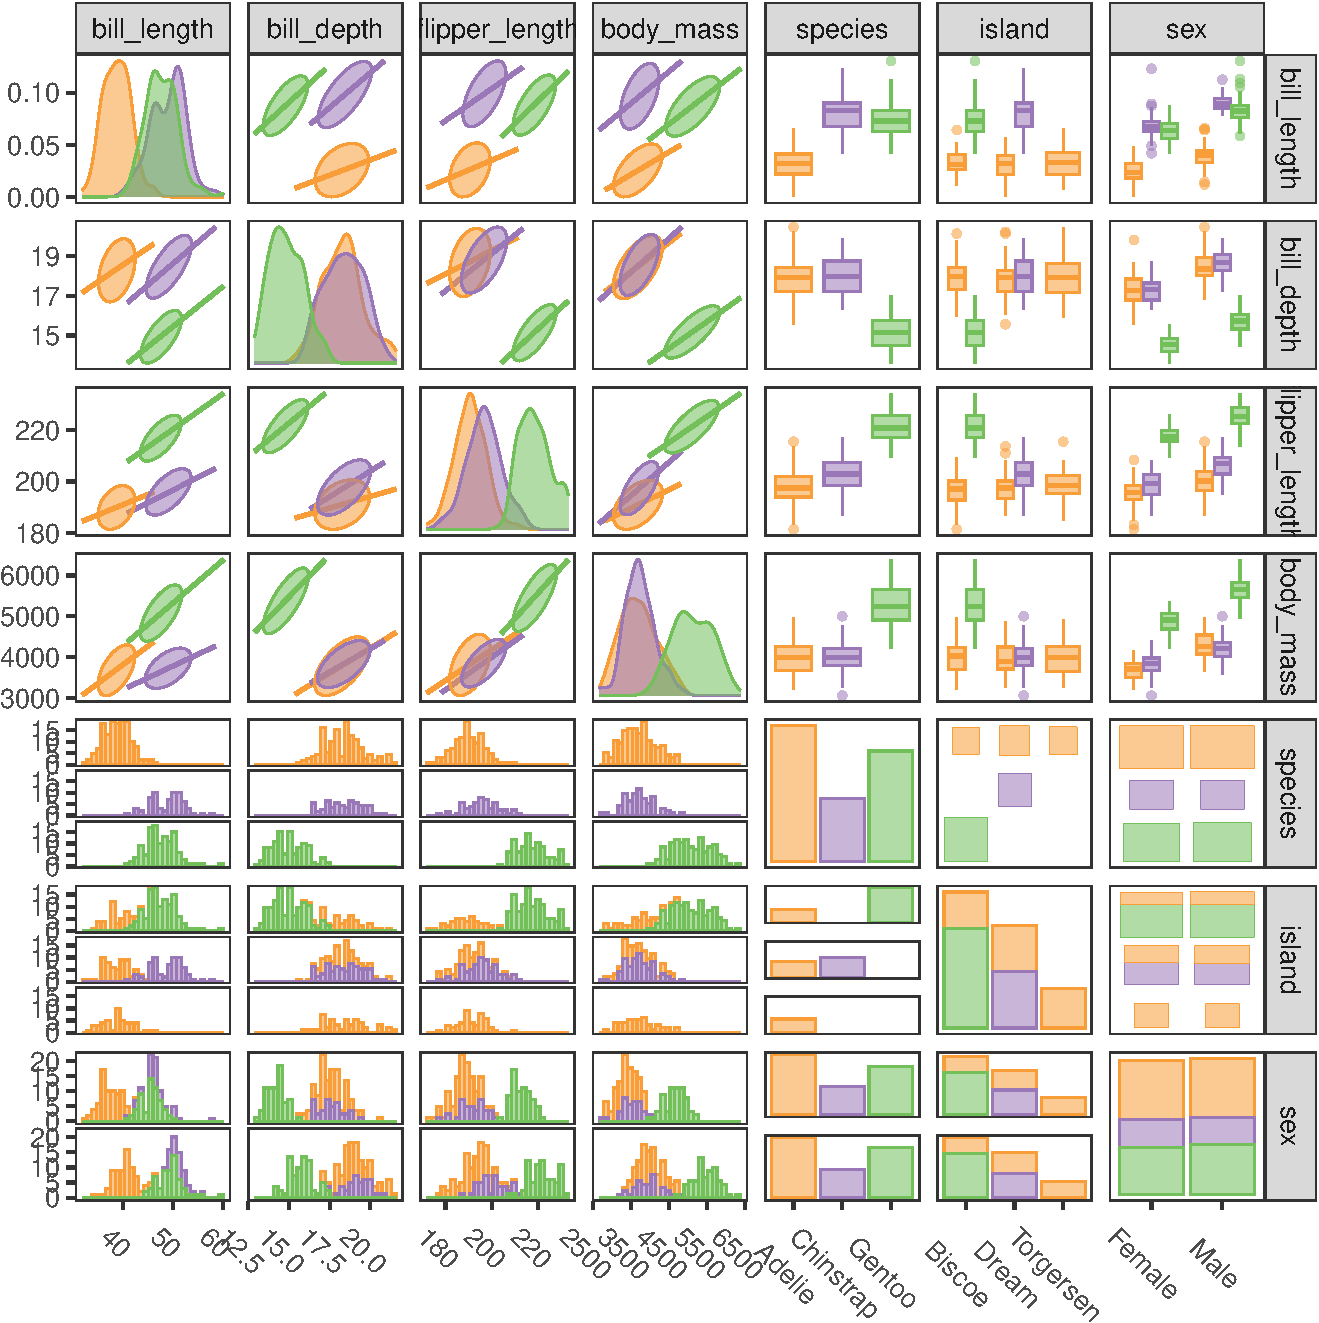
\includegraphics[width=1\textwidth,height=\textheight]{figs/ch03/fig-peng-ggpairs7-1.pdf}

}

\caption{\label{fig-peng-ggpairs7}Customized \texttt{ggpairs()} plot of
penguin size variables, together with species, island and sex.}

\end{figure}

There is certainly a lot going on in Figure~\ref{fig-peng-ggpairs7}, but
it does show a high-level overview of all the variables (except
\texttt{year}) in the penguins dataset.

\hypertarget{sec-parcoord}{%
\section{Parallel coordinate plots}\label{sec-parcoord}}

As we have seen above, scatterplot matrices and generalized pairs plots
extend data visualization to multivariate data, but these variables
share one 2D space, so resolution decreases as the number of variable
increase. You need a very large screen or sheet of paper to see more
than, say 5-6 variables with any clarity.

Parallel coordinate plots are an attractive alternative, with which we
can visualize an arbitrary number of variables to get a visual summary
of a potentially high-dimensional dataset, and perhaps recognize
outliers and clusters in the data in a different way. In these plots,
each variable is shown on a separate, parallel axis. A multivariate
observation is then plotted by connecting their respective values on
each axis with lines across all the axes.

The geometry of parallel coordinates is interesting, because what is a
point in \(n\)-dimensional (Euclidean) \emph{data} space becomes a line
in the \emph{projective} parallel coordinate space with \(n\) axes, and
vice-versa: lines in parallel coordinate space correspond to points in
data space. Thus, a collection of points in data space map to lines that
intersect in a point in projective space. What this does is to map
\(n\)-dimensional relations into 2D patterns we can see in a parallel
coordinates plot.

\begin{tcolorbox}[enhanced jigsaw, colback=white, rightrule=.15mm, left=2mm, arc=.35mm, colframe=quarto-callout-note-color-frame, toptitle=1mm, breakable, leftrule=.75mm, opacityback=0, bottomtitle=1mm, colbacktitle=quarto-callout-note-color!10!white, opacitybacktitle=0.6, titlerule=0mm, toprule=.15mm, title=\textcolor{quarto-callout-note-color}{\faInfo}\hspace{0.5em}{History Corner}, bottomrule=.15mm, coltitle=black]

\begin{quote}
Those who don't know history are doomed to plagarize it ---The author
\end{quote}

The theory of projective geometry originated with the French
mathematician Maurice d'Ocagne
(\protect\hyperlink{ref-Ocagne:1885}{1885}) who sought a way to provide
graphic calculation of mathematical functions with alignment diagrams or
\emph{nomograms} using parallel axes with different scales. A
three-variable equation, for example, could be solved using three
parallel axes, where known values could be marked on their scales, a
line drawn between them, and an unknown read on its scale at the point
where the line intersects that scale.

Henry Gannet (1880), in work preceding the \emph{Statistical Atlas of
the United States} for the 1890 Census
(\protect\hyperlink{ref-Gannett:1898}{Gannett, 1898}), is widely
credited with being the first to use parallel coordinates plots to show
data, in his case, to show the
\href{https://www.davidrumsey.com/luna/servlet/detail/RUMSEY~8~1~32803~1152181}{rank
ordering of US states} by 10 measures including population, occupations,
wealth, manufacturing, agriculture and so on.

However, both d'Ocagne and Gannet were far preceded in this by
Andre-Michel Guerry (\protect\hyperlink{ref-Guerry:1833}{1833}) who used
this method to show how the rank order of various crimes changed with
age of the accused. See Friendly
(\protect\hyperlink{ref-Friendly2022}{2022}), Figure 7 for his version
and for an appreciation of the remarkable contributions of this amateur
statistician to the history of data visualization.

The use of parallel coordinates for display of multidimensional data was
rediscovered by Alfred Inselberg
(\protect\hyperlink{ref-Inselberg:1985}{1985}) and extended by Edward
Wegman (\protect\hyperlink{ref-Wegman:1990}{1990}), neither of whom
recognized the earlier history. Somewhat earlier, David Andrews
(\protect\hyperlink{ref-Andrews:72}{1972}) proposed mapping multivariate
observations to smooth Fourrier functions composed of alternating
\(\sin()\) and \(\cos()\) terms. And in my book, \emph{SAS System for
Statistical Graphics} (\protect\hyperlink{ref-Friendly:91}{Friendly,
1991}), I implemented what I called
\href{https://blogs.sas.com/content/iml/2022/11/14/profile-plots-sas.html}{\emph{profile
plots}} without knowing their earlier history as parallel coordinate
plots.

\end{tcolorbox}

Parallel coordinate plots present a challenge for graphic developers, in
that they require a different way to think about plot construction for
multiple variables, which can be quantitative, as in the original idea,
or categorical factors, all to be shown along parallel axes.

Here, I use the \textbf{ggpcp} package
(\protect\hyperlink{ref-R-ggpcp}{Hofmann et al., 2022}), best described
in VanderPlas et al. (\protect\hyperlink{ref-VanderPlas2023}{2023}), who
also review the modern history. This takes some getting used to, because
they develop \texttt{pcp\_*()} extensions of the \texttt{ggplot2}
grammar of graphics framework to allow:

\begin{itemize}
\tightlist
\item
  \texttt{pcp\_select()}: selections of the variables to be plotted and
  their horizontal order on parallel axes,
\item
  \texttt{pcp\_scale()}: methods for scaling of the variables to each
  axis,
\item
  \texttt{pcp\_arrange()}: methods for breaking ties in factor variables
  to space them out.
\end{itemize}

Then, it provides \texttt{geom\_pcp\_*()} functions to control the
display of axes with appropriate aesthetics, labels for categorical
factors and so forth. \textbf{?@fig-peng-ggpcp1} illustrates this type
of display, using sex and species in addition to the quantitative
variables for the penguin data.

\begin{Shaded}
\begin{Highlighting}[]
\NormalTok{peng }\SpecialCharTok{|\textgreater{}}
  \FunctionTok{pcp\_select}\NormalTok{(bill\_length}\SpecialCharTok{:}\NormalTok{body\_mass, sex, species) }\SpecialCharTok{|\textgreater{}}
  \FunctionTok{pcp\_scale}\NormalTok{(}\AttributeTok{method =} \StringTok{"uniminmax"}\NormalTok{) }\SpecialCharTok{|\textgreater{}}
  \FunctionTok{pcp\_arrange}\NormalTok{() }\SpecialCharTok{|\textgreater{}}
  \FunctionTok{ggplot}\NormalTok{(}\FunctionTok{aes\_pcp}\NormalTok{()) }\SpecialCharTok{+}
  \FunctionTok{geom\_pcp\_axes}\NormalTok{() }\SpecialCharTok{+}
  \FunctionTok{geom\_pcp}\NormalTok{(}\FunctionTok{aes}\NormalTok{(}\AttributeTok{colour =}\NormalTok{ species), }\AttributeTok{alpha =} \FloatTok{0.8}\NormalTok{, }\AttributeTok{overplot =} \StringTok{"none"}\NormalTok{) }\SpecialCharTok{+}
  \FunctionTok{geom\_pcp\_labels}\NormalTok{() }\SpecialCharTok{+}
  \FunctionTok{scale\_colour\_manual}\NormalTok{(}\AttributeTok{values =} \FunctionTok{peng.colors}\NormalTok{()) }\SpecialCharTok{+}
  \FunctionTok{labs}\NormalTok{(}\AttributeTok{x =} \StringTok{""}\NormalTok{, }\AttributeTok{y =} \StringTok{""}\NormalTok{) }\SpecialCharTok{+}
  \FunctionTok{theme}\NormalTok{(}\AttributeTok{axis.title.y =} \FunctionTok{element\_blank}\NormalTok{(), }\AttributeTok{axis.text.y =} \FunctionTok{element\_blank}\NormalTok{(), }
        \AttributeTok{axis.ticks.y =} \FunctionTok{element\_blank}\NormalTok{(), }\AttributeTok{legend.position =} \StringTok{"none"}\NormalTok{)}
\end{Highlighting}
\end{Shaded}

\begin{figure}

{\centering 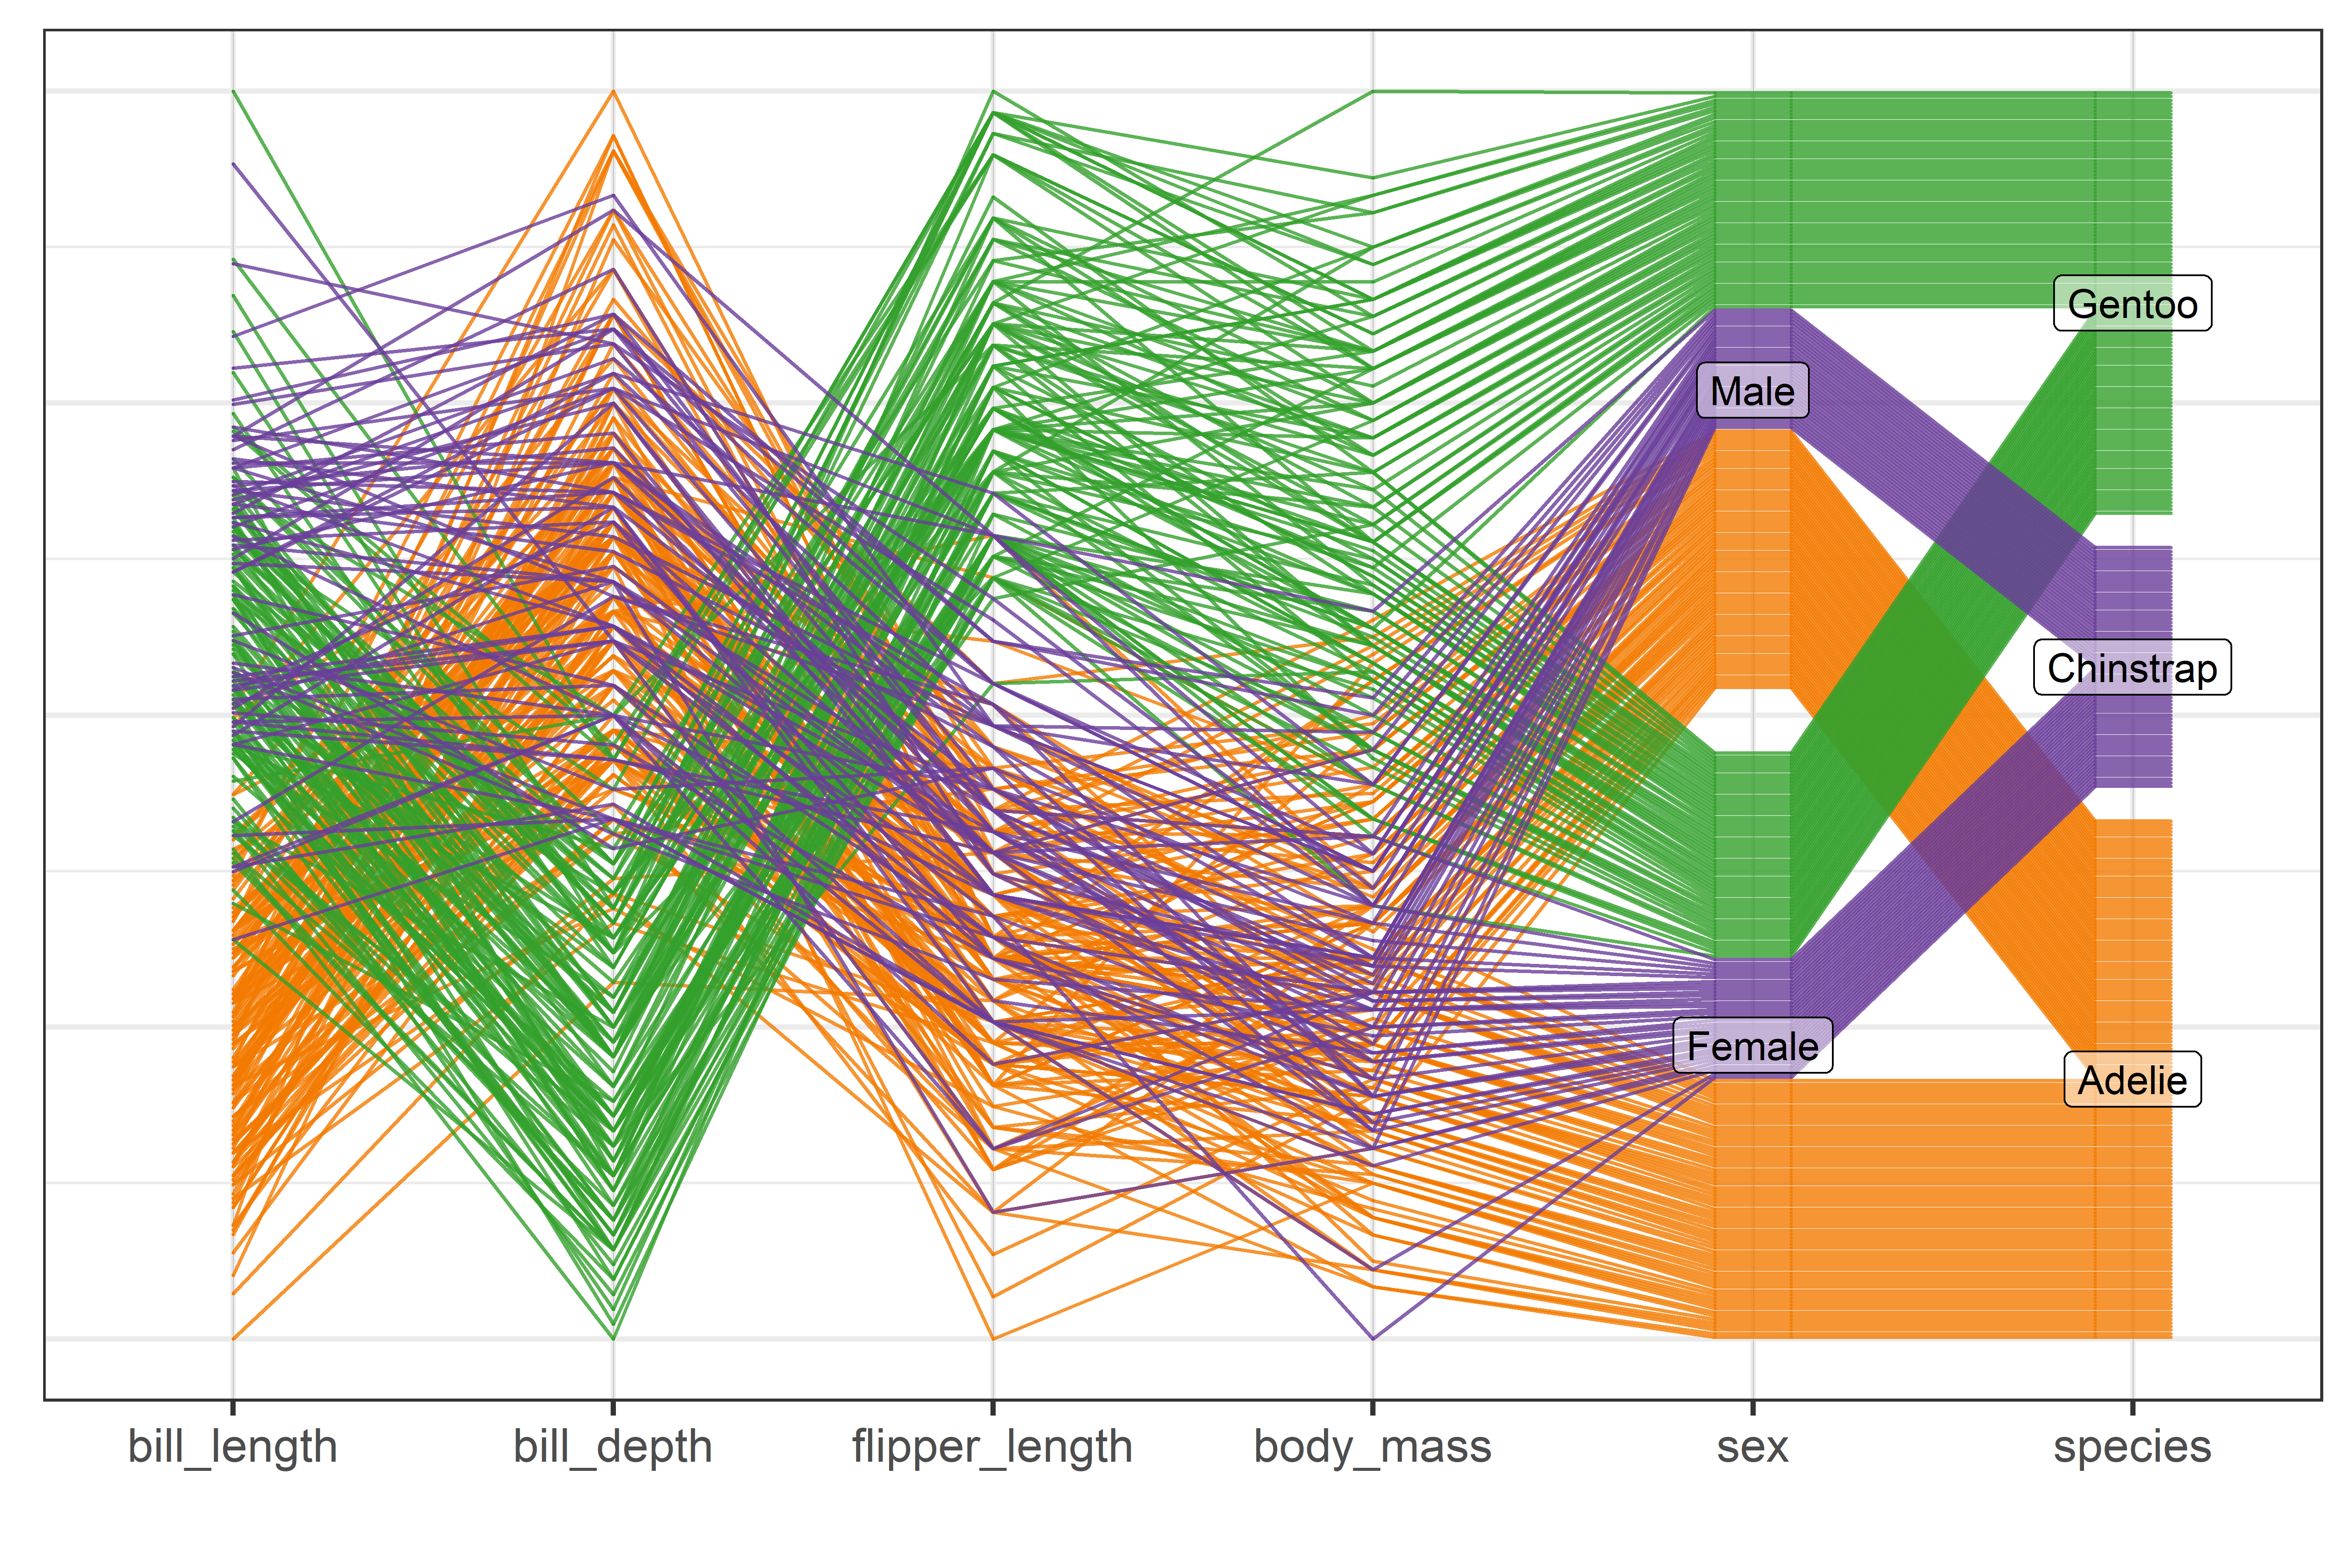
\includegraphics[width=18in,height=\textheight]{figs/fig-peng-ggpcp1-1.png}

}

\end{figure}

Rearranging the order of variables and the ordering of factor levels can
make a difference in what we can see in such plots. For a simple example
(following VanderPlas et al.
(\protect\hyperlink{ref-VanderPlas2023}{2023})), we reorder the levels
of species and islands to make it clearer which species occur on each
island.

\begin{Shaded}
\begin{Highlighting}[]
\NormalTok{peng1 }\OtherTok{\textless{}{-}}\NormalTok{ peng }\SpecialCharTok{|\textgreater{}}
  \FunctionTok{mutate}\NormalTok{(}\AttributeTok{species =} \FunctionTok{factor}\NormalTok{(species, }\AttributeTok{levels =} \FunctionTok{c}\NormalTok{(}\StringTok{"Chinstrap"}\NormalTok{, }\StringTok{"Adelie"}\NormalTok{, }\StringTok{"Gentoo"}\NormalTok{))) }\SpecialCharTok{|\textgreater{}}
  \FunctionTok{mutate}\NormalTok{(}\AttributeTok{island =} \FunctionTok{factor}\NormalTok{(island, }\AttributeTok{levels =} \FunctionTok{c}\NormalTok{(}\StringTok{"Dream"}\NormalTok{, }\StringTok{"Torgersen"}\NormalTok{, }\StringTok{"Biscoe"}\NormalTok{)))}

\NormalTok{peng1 }\SpecialCharTok{|\textgreater{}}
  \FunctionTok{pcp\_select}\NormalTok{(species, island, bill\_length}\SpecialCharTok{:}\NormalTok{body\_mass) }\SpecialCharTok{|\textgreater{}}
  \FunctionTok{pcp\_scale}\NormalTok{() }\SpecialCharTok{|\textgreater{}}
  \FunctionTok{pcp\_arrange}\NormalTok{(}\AttributeTok{method =} \StringTok{"from{-}left"}\NormalTok{) }\SpecialCharTok{|\textgreater{}}
  \FunctionTok{ggplot}\NormalTok{(}\FunctionTok{aes\_pcp}\NormalTok{()) }\SpecialCharTok{+}
  \FunctionTok{geom\_pcp\_axes}\NormalTok{() }\SpecialCharTok{+}
  \FunctionTok{geom\_pcp}\NormalTok{(}\FunctionTok{aes}\NormalTok{(}\AttributeTok{colour =}\NormalTok{ species), }\AttributeTok{alpha =} \FloatTok{0.6}\NormalTok{, }\AttributeTok{overplot =} \StringTok{"none"}\NormalTok{) }\SpecialCharTok{+}
  \FunctionTok{geom\_pcp\_boxes}\NormalTok{(}\AttributeTok{fill =} \StringTok{"white"}\NormalTok{, }\AttributeTok{alpha =} \FloatTok{0.5}\NormalTok{) }\SpecialCharTok{+}
  \FunctionTok{geom\_pcp\_labels}\NormalTok{() }\SpecialCharTok{+}
  \FunctionTok{scale\_colour\_manual}\NormalTok{(}\AttributeTok{values =} \FunctionTok{peng.colors}\NormalTok{()[}\FunctionTok{c}\NormalTok{(}\DecValTok{2}\NormalTok{,}\DecValTok{1}\NormalTok{,}\DecValTok{3}\NormalTok{)]) }\SpecialCharTok{+}
  \FunctionTok{theme\_bw}\NormalTok{() }\SpecialCharTok{+}
  \FunctionTok{labs}\NormalTok{(}\AttributeTok{x =} \StringTok{""}\NormalTok{, }\AttributeTok{y =} \StringTok{""}\NormalTok{) }\SpecialCharTok{+}
  \FunctionTok{theme}\NormalTok{(}\AttributeTok{axis.text.y =} \FunctionTok{element\_blank}\NormalTok{(), }\AttributeTok{axis.ticks.y =} \FunctionTok{element\_blank}\NormalTok{(),}
        \AttributeTok{legend.position =} \StringTok{"none"}\NormalTok{) }
\end{Highlighting}
\end{Shaded}

\begin{figure}

{\centering 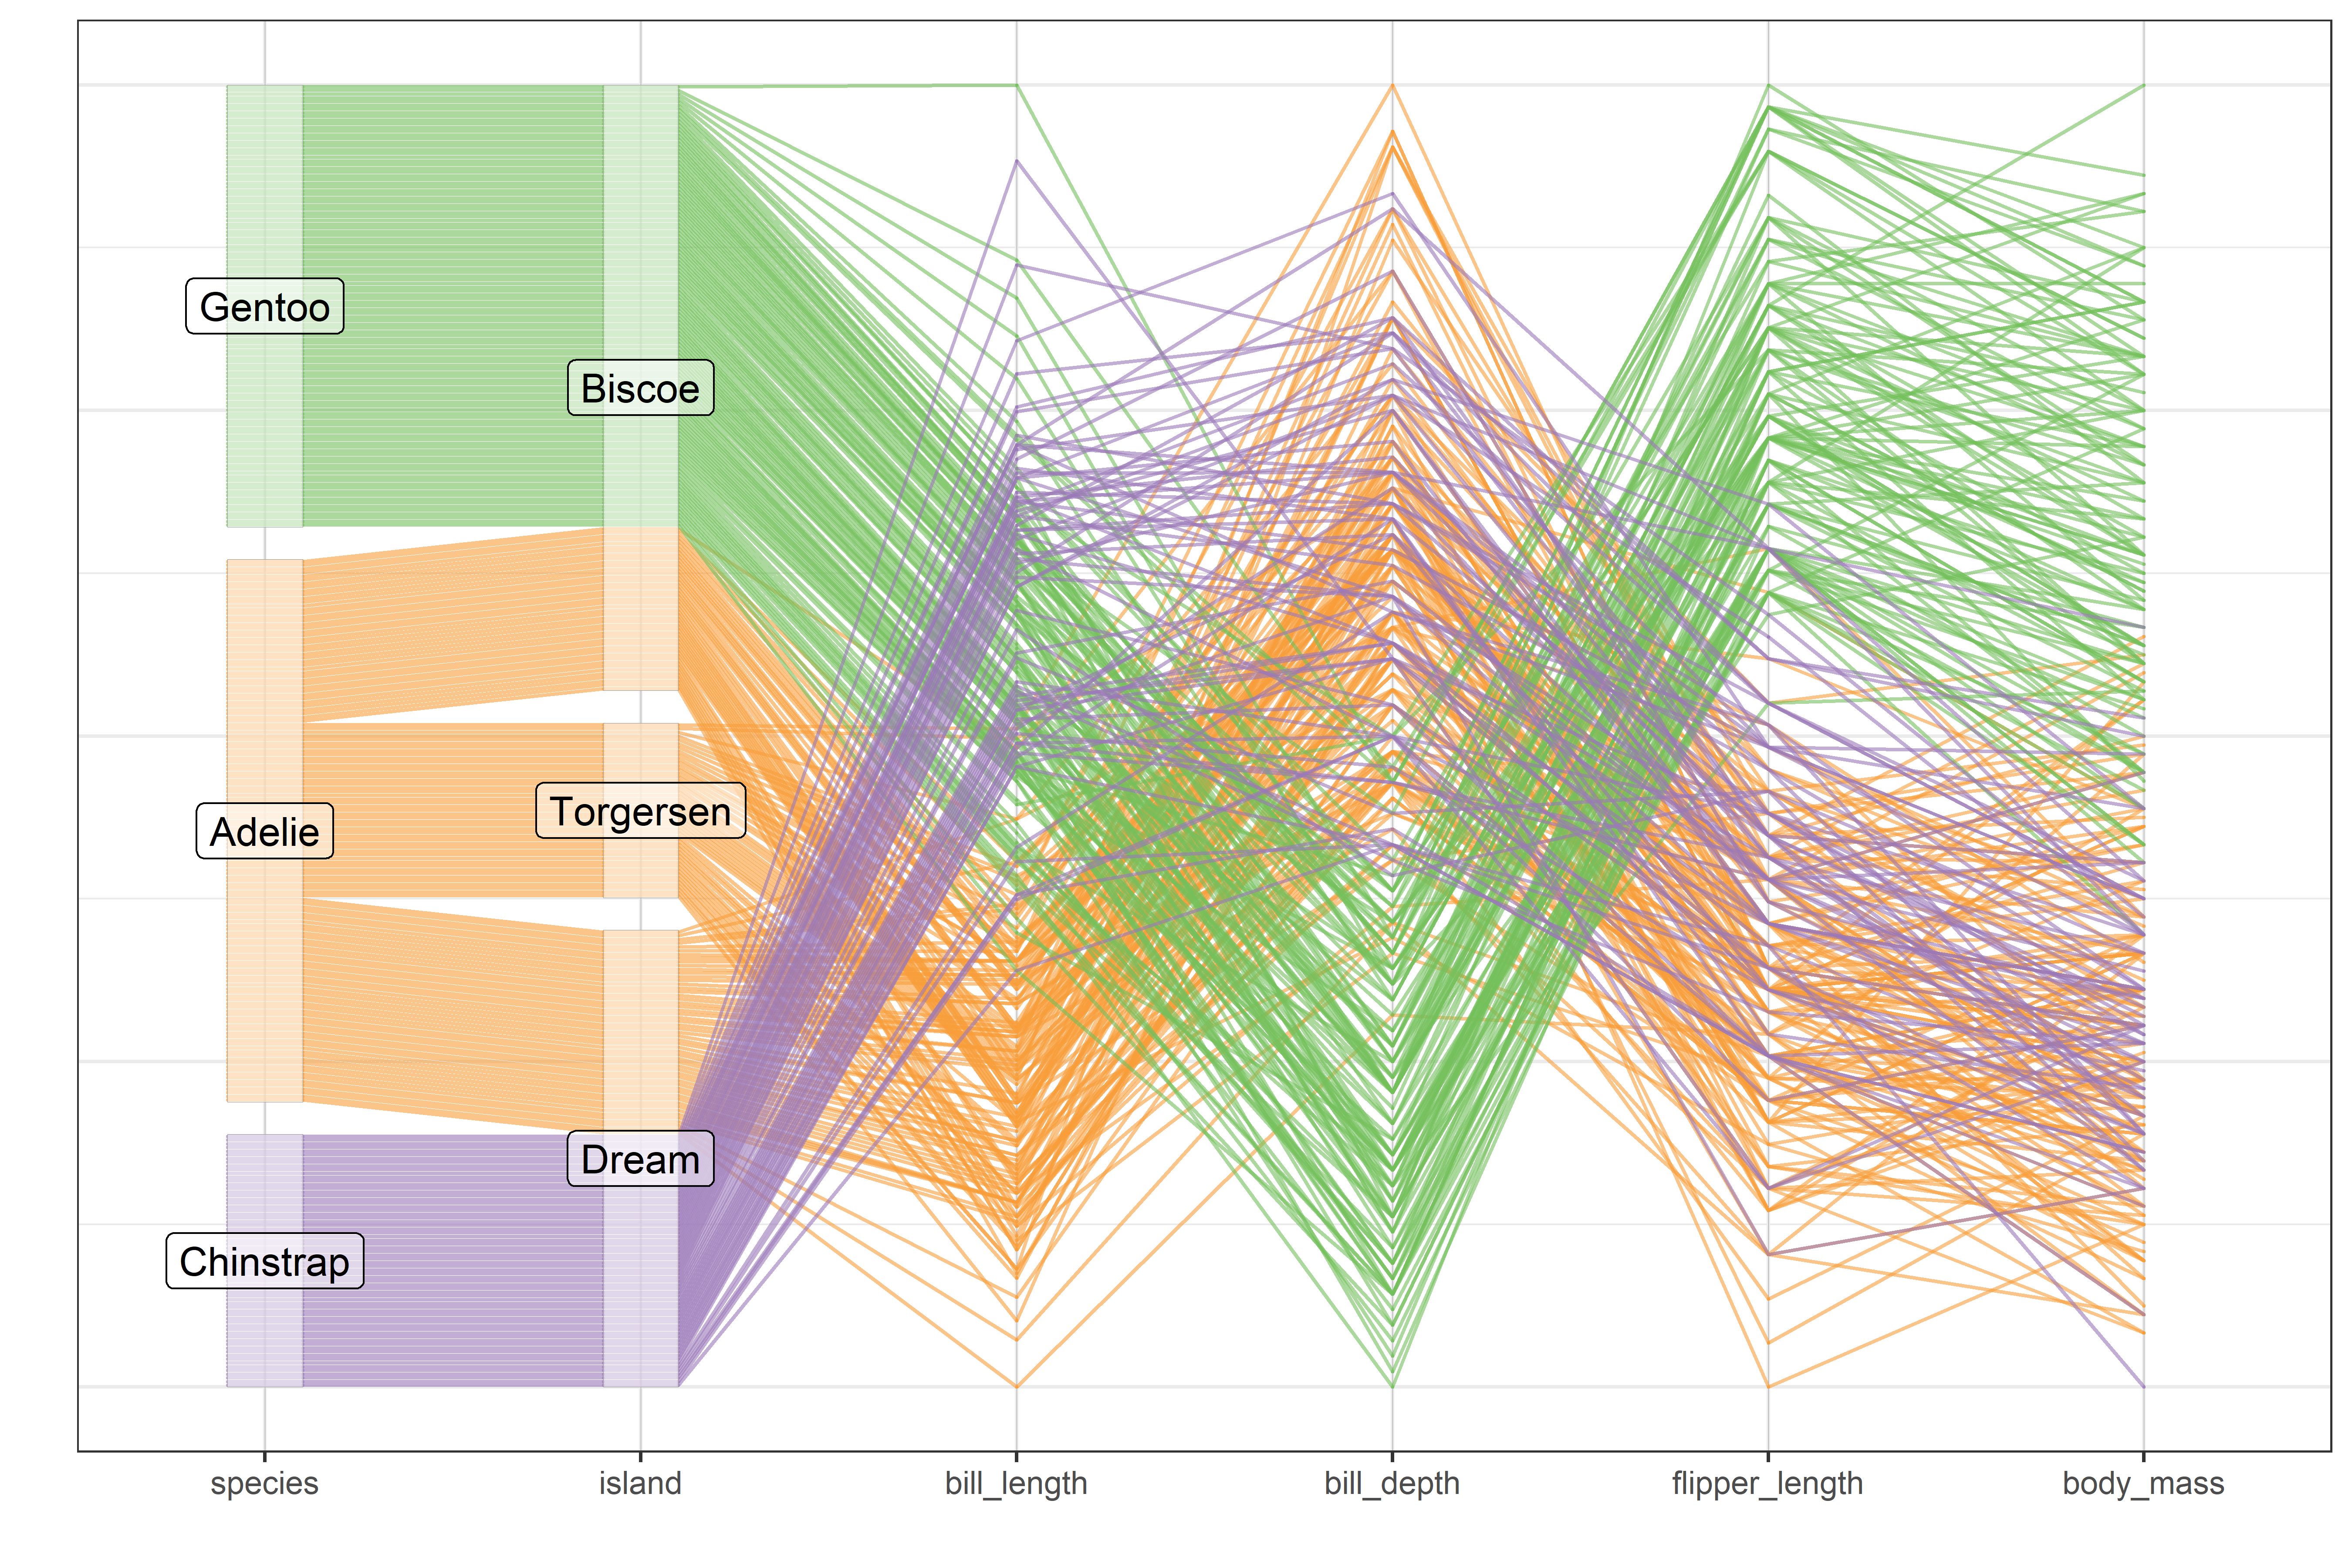
\includegraphics[width=18in,height=\textheight]{figs/fig-peng-ggpcp2-1.png}

}

\end{figure}

This plot emphasizes the relation between penguin species and the island
where they were observed and then shows the values of the quantitative
body size measurements.

Packages used here: 21 packages used here: base, car, carData, corrgram,
corrplot, datasets, dplyr, GGally, ggdensity, ggpcp, ggplot2, graphics,
grDevices, grid, knitr, methods, patchwork, stats, tidyr, utils, vcd

\bookmarksetup{startatroot}

\hypertarget{sec-pca-biplot}{%
\chapter{PCA and Biplots}\label{sec-pca-biplot}}

\hypertarget{sec-spaceland}{%
\section{\texorpdfstring{\emph{Flatland} and
\emph{Spaceland}}{Flatland and Spaceland}}\label{sec-spaceland}}

\begin{quote}
It is high time that I should pass from these brief and discursive notes
about Flatland to the central event of this book, my initiation into the
mysteries of Space. THAT is my subject; all that has gone before is
merely preface --- Edwin Abbott, \emph{Flatland}, p.~57.
\end{quote}

There was a cloud in the sky above \emph{Flatland} one day. But it was a
huge, multidimensional cloud of sparkly points that might contain some
important message, perhaps like the hidden EUREKA
(Figure~\ref{fig-pollen-eureka-fig}), or perhaps forecasting the
upcoming harvest, if only Flatlanders could appreciate it.

A leading citizen, A SQUARE, who had traveled once to Spaceland and
therefore had an inkling of its majesty beyond the simple world of his
life in the plane looked at that cloud and had a brilliant thought, an
OMG moment:

\begin{quote}
``Oh, can I, in my imagination, rotate that cloud and squeeze its' juice
so that it rains down on Flatland with greatest joy?''
\end{quote}

As it happened, our Square friend, although he could never really
\emph{see} in three dimensions, he could now at least \emph{think} of a
world described by \textbf{height} as well as breadth and width, and
think of the \textbf{shadow} cast by a cloud as something mutable,
changing size and shape depending on its' orientation over Flatland.

And what a world it was, inhabited by Pryamids, Cubes and wondrous
creatures called Polyhedrons with many \(C\)orners, \(F\)aces and
\(E\)dges. Not only that, but all those Polyhedra were forced in
Spaceland to obey a magic formula: \(C + F - E = 2\).\footnote{This is
  Euler's (\protect\hyperlink{ref-Euler:1758}{1758}) formula, which
  states that any convex polyheron must obey the formula
  \(V + F - E = 2\) where \(V\) is the number of vertexes (corners),
  \(F\) is the number of faces and \(E\) is the number of edges. For
  example, a tetrahedron or pyramid has \((V, F, E) = (4, 4, 6)\) and a
  cube has \((V, F, E) = (8, 6, 12)\). Stated in words, for all solid
  bodies confined by planes, the sum of the number of vertexes and the
  number of faces is two less than the number of edges.} How cool was
that!

Indeed, there were even exalted Spheres, having so many faces that its
surface became as smooth as a baby's bottom with no need for pointed
corners or edges, just as Circles were the smoothest occupants of his
world with far too many sides to count. It was his dream of a Sphere
passing through Flatland (Figure~\ref{fig-flatland-spheres}) that first
awakened him to a third dimension.

He also marveled at Ellipsoids, as smooth as Spheres, but in Spaceland
having three natural axes of different extent and capable of being
appearing fatter or slimmer when rotated from different views. An
Ellipsoid had magical properties: it could appear as so thin in one or
more dimensions that it became a simple 2D ellipse, or a 1D line, or
even a 0D point
(\protect\hyperlink{ref-Friendly-etal:ellipses:2013}{Friendly et al.,
2013}).

All of these now arose in Square's richer 3D imagination. And, all of
this came from just one more dimension than his life in Flatland.

\hypertarget{multivariate-juicers}{%
\subsection{Multivariate juicers}\label{multivariate-juicers}}

Up to now, we have also been living in Flatland. We have been trying to
understand data in \textbf{data space} of possibly many dimensions, but
confined to the 2D plane of a graph window. Scatterplot matrices and
parallel coordinate plots provided some relief. The former did so by
\textbf{projecting} the data into sets of 2D views in the coordinates of
data space; the latter did so by providing multiple axes in a 2D space
along which we could trace the paths of individual observations.

This chapter is about seeing data in a different projection, a
low-dimensional, usually 2D, space that which squeezes out the most
juice from multidimensional data for a particular purpose
(Figure~\ref{fig-MV-juicer}), where what we want to understand can be
more easily seen.

\begin{figure}

{\centering 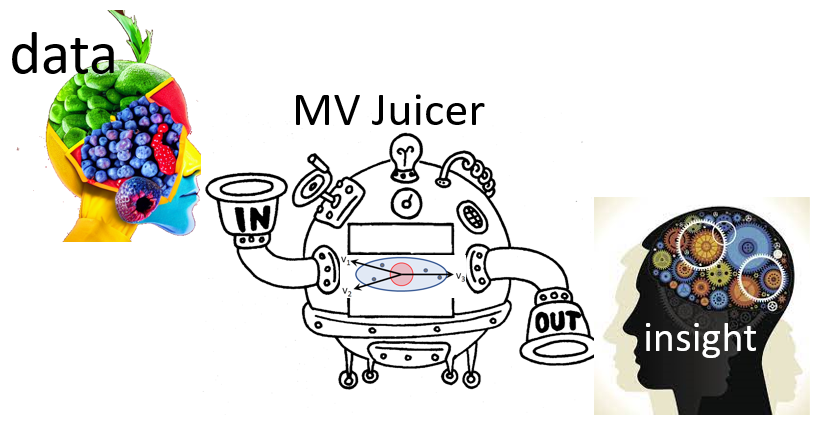
\includegraphics[width=0.9\textwidth,height=\textheight]{images/MV-juicer.png}

}

\caption{\label{fig-MV-juicer}A multivariate juicer takes data from
possibly high-dimensional data space and transforms it to a
lower-dimenional space in which important effects can be more easily
seen.}

\end{figure}

Here, I concentrate on \textbf{principal components analysis} (PCA),
whose goal reflects A Square's desire to see that sparkly cloud of
points in \(nD\) space in the plane showing the greatest variation
(squeezing the most juice) among all other possible views. This appealed
to his sense of geometry, but left him wondering how the variables in
that high-D cloud were related to the dimensions he could see in a
best-fitting plane.

The idea of a \textbf{biplot}, showing the data points in the plane,
together with thick pointed arrows---variable vectors--- in one view is
the other topic explained in this chapter (Section~\ref{sec-biplot}).
The biplot is the simplest example of a multivariate juicer. The
essential idea is to project the cloud of data points in \(n\)
dimensions into the 2D space of principal components and simultaneously
show how the original variables relate to this space. For exploratory
analysis to get an initial, incisive view of a multivariate dataset, a
biplot is often my first choice.

\begin{tcolorbox}[enhanced jigsaw, colback=white, rightrule=.15mm, left=2mm, arc=.35mm, colframe=quarto-callout-note-color-frame, toptitle=1mm, breakable, leftrule=.75mm, opacityback=0, bottomtitle=1mm, colbacktitle=quarto-callout-note-color!10!white, opacitybacktitle=0.6, titlerule=0mm, toprule=.15mm, title=\textcolor{quarto-callout-note-color}{\faInfo}\hspace{0.5em}{Looking ahead}, bottomrule=.15mm, coltitle=black]

I'm using the term \emph{multivariate juicer} here to refer the wider
class of \textbf{dimension reduction} techniques, used for various
purposes in data analysis and visualization. Principal components
analysis is the simplest example and illustrates the general ideas.

The key point is that these methods are designed to transform the data
into a low-dimensional space for a particular goal or purpose. In PCA,
the goal is to extract the greatest amount of total variability in the
data. In the context of univariate multiple regression, the goal is
often to reduce the number of predictors necessary to account for an
outcome variable, called \emph{feature extraction} in the machine
learning literature.

When the goal is to best distinguish among groups \textbf{discriminant
analysis} finds uncorrelated weighted sums of predictors on which the
means of groups are most widely separated in a reduced space of
hopefully fewer dimensions.

The methods I cover in this book are all linear methods, but there is
also a wide variety of non-linear dimension reduction techniques
\ldots{}

\end{tcolorbox}

\textbf{Packages}

In this chapter I use the following packages. Load them now:

\begin{Shaded}
\begin{Highlighting}[]
\FunctionTok{library}\NormalTok{(ggplot2)}
\FunctionTok{library}\NormalTok{(dplyr)}
\FunctionTok{library}\NormalTok{(tidyr)}
\FunctionTok{library}\NormalTok{(patchwork)}
\FunctionTok{library}\NormalTok{(ggbiplot)}
\FunctionTok{library}\NormalTok{(FactoMineR)}
\FunctionTok{library}\NormalTok{(factoextra)}
\end{Highlighting}
\end{Shaded}

\hypertarget{sec-pca}{%
\section{Principal components analysis}\label{sec-pca}}

When Francis Galton (\protect\hyperlink{ref-Galton:1886}{1886}) first
discovered the idea of regression toward the mean and presented his
famous diagram (Figure~\ref{fig-galton-corr}), he had little thought
that he had provided a window to a higher-dimensional world, beyond what
even A Square could imagine. His friend, Karl Pearson
(\protect\hyperlink{ref-Pearson:1896}{1896}) took that idea and
developed it into a theory of regression and a measure of correlation
that would bear his name, Pearson's \(r\).

But then Pearson (\protect\hyperlink{ref-Pearson:1901}{1901}) had a
further inspiration, akin to that of A Square. If he also had a cloud of
sparkly points in \(2, 3, 4, ..., p\) dimensions, could he find a point
(\(0D\)), or line (\(1D\)), or plane (\(2D\)), or even a hyperplane
(\(nD\)) that best summarized --- squeezed out the most juice---from
multivariate data? This was the first trully multivariate problem in the
history of statistics
(\protect\hyperlink{ref-FriendlyWainer:2021:TOGS}{Friendly \& Wainer,
2021, p. 186}).

The best \(0D\) point was easy--- it was simply the centroid, the means
of each of the variables in the data,
\((\bar{x}_1, \bar{x}_2, ..., \bar{x}_p)\), because that was ``closest''
to the data in the sense of minimizing the sum of squared differences,
\(\Sigma_i\Sigma_j (x_{ij} - \bar{x}_j)^2\). In higher dimensions, his
solution was also an application of the method of least squares, but he
argued it geometrically and visually as shown in
Figure~\ref{fig-Pearson1901}.

\begin{figure}

{\centering 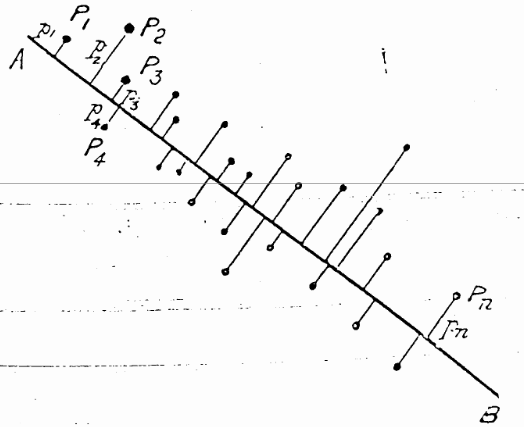
\includegraphics[width=0.7\textwidth,height=\textheight]{images/Pearson1901.png}

}

\caption{\label{fig-Pearson1901}Karl Pearson's (1901) geometric, visual
argument for finding the line or plane of closest fit to a collection of
points, P1, P2, P3, \ldots{}}

\end{figure}

For a \(1D\) summary, the line of best fit to the points
\(P_1, P_2, \dots P_n\) is the line that goes through the centroid and
made the average squared length of the \emph{perpendicular} segments
from those points to a line as small as possible. This was different
from the case in linear regression, for fitting \(y\) from \(x\), where
the average squared length of the \emph{vertical} segments,
\(\Sigma_i (y_i - \hat{y}_i)^2\) was minimized by least squares.

He went on to prove the visual insights from simple smoothing of Galton
(\protect\hyperlink{ref-Galton:1886}{1886}) (shown in
Figure~\ref{fig-galton-corr}) regarding the regression lines of
\texttt{y\ \textasciitilde{}\ x} and \texttt{x\ \textasciitilde{}\ y}.
More importantly, he proved that the cloud of points is captured, for
the purpose of finding a best line, plane or hyperplane, by the
ellipsoid that encloses it, as seen in his diagram,
Figure~\ref{fig-Pearson1901-2}. The major axis of the 2D ellipse is the
line of best fit, along which the data points have the smallest average
squared distance from the line. The axis at right angles to that---the
minor axis--- is labeled ``line of worst fit'' with the largest average
squared distance.

\begin{figure}

{\centering 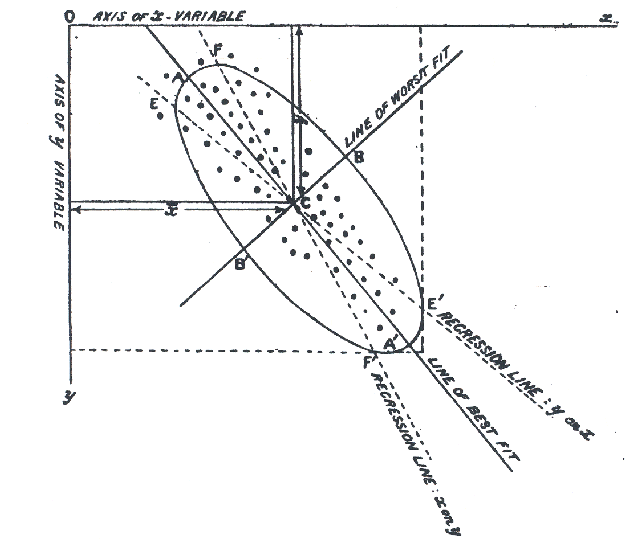
\includegraphics[width=0.8\textwidth,height=\textheight]{images/Pearson1901_2.png}

}

\caption{\label{fig-Pearson1901-2}Karl Pearson's diagram showing the
elliptical geometry of regression and principal components analysis
\ldots{} \emph{Source}: Pearson (1901), p.~566.}

\end{figure}

Even more importantly--- and this is the basis for what we call
\textbf{principal components analysis} (PCA)--- he recognized that the
two orthogonal axes of the ellipse gave new coordinates for the data
which were uncorrelated, whatever the correlation of \(x\) and \(y\).

\begin{quote}
Physically, the axes of the correlation type-ellipse are the directions
of independent and uncorrelated variation. --- Pearson
(\protect\hyperlink{ref-Pearson:1901}{1901}), p.~566.
\end{quote}

It was but a small step to recognize that for two variables, \(x\) and
\(y\):

\begin{itemize}
\tightlist
\item
  the line of best fit, the major axis (PC1) had the greatest variance
  of points projected onto it;
\item
  the line of worst fit, the minor axis (PC2), had the least variance;
\item
  these could be seen as a rotation of the data space of \((x, y)\) to a
  new space (PC1, PC2) with uncorrelated variables;
\item
  the total variation of the points in data space,
  \(\text{Var}(x) + \text{Var}(y)\), being unchanged by rotation, was
  equally well expressed as the total variation
  \(\text{Var}(PC1) + \text{Var}(PC2)\) of the scores on what are now
  called the principal component axes.
\end{itemize}

It would have appealed to Pearson (and also to A Square) to see these
observations demonstrated in a 3D video. \textbf{?@fig-pca-animation}
shows a 3D plot of the variables \texttt{Sepal.Length},
\texttt{Sepal.Width} and \texttt{Petal.Length} in Edgar Anderson's
\texttt{iris} data, with points colored by species and the 95\% data
ellipsoid. This is rotated smoothly by interpolation until the first two
principal axes, PC1 and PC2 are aligned with the horizontal and vertical
dimensions. Because this is a rigid rotation of the cloud of points, the
total variability is obviously unchanged.

\hypertarget{pca-by-springs}{%
\subsection{PCA by springs}\label{pca-by-springs}}

Before delving into the mathematics of PCA, it is useful to see how
Pearson's problem, and fitting by least squares generally, could be
solved in a physical realization.

From elementary statistics, you may be familiar with a physical
demonstration that the mean, \(\bar{x}\), of a sample is the value for
which the sum of deviations, \(\Sigma_i (x_i - \bar{x})\) is zero, so
the mean can be visualized as the point of balance on a line where those
differences \((x_i - \bar{x})\) are placed. Equally well, there is a
physical realization of the mean as the point along an axis where
weights connected by springs will minimize the sum of squared
differences, because springs with a constant stiffness, \(k\), exert
forces proportional to \(k (x_i - \bar{x}) ^2\). That's the reason is
useful as a measure of central tendency: it minimizes the average
squared error.

In two dimensions, imagine that we have points, \((x_i, y_i)\) and these
are attached by springs of equal stiffness \(k\), to a line anchored at
the centroid, \((\bar{x}, \bar{y})\) as shown in
Figure~\ref{fig-pca-springs}. If we rotate the line to some initial
position and release it, the springs will pull the line clockwise or
counterclockwise and the line will bounce around until the forces,
proportional to the squares of the lengths of the springs, will
eventually balance out at the position (shown by the
\textcolor{red}{red} fixed line segments at the ends). This is the
position that minimizes the the sum of squared lengths of the connecting
springs, and also minimizes the kinetic energy in the system.

If you look closely at Figure~\ref{fig-pca-springs} you will see
something else: When the line is at its' final position of minimum
squared length and energy, the positions of the \textcolor{red}{red}
points on this line are spread out furthest, i.e., have \textbf{maximum}
variance. Conversely, when the line line is at right angles to its'
final position (shown by the black line at 90\(^o\)) the projected
points have the smallest possible variance.

\begin{figure}

{\centering 

}

\caption{\label{fig-pca-springs}Animation of PCA fitted by springs. The
\textcolor{blue}{blue} data points are connected to their projections on
the \textcolor{red}{red} line by springs perpendicular to that line.
From an initial position, the springs pull that line in proportion to
their squared distances, until the line finally settles down to the
position where the forces are balanced and the minimum is achieved.
\emph{Source}: Amoeba, https://bit.ly/46tAicu.}

\end{figure}

\textbf{TODO}: Simple PCA example using workers data

\hypertarget{mathematics-and-geometry-of-pca}{%
\subsection{Mathematics and geometry of
PCA}\label{mathematics-and-geometry-of-pca}}

As the ideas of principal components developed, there was a happy
marriage of Galton's geometrical intuition and Pearson's mathematical
analysis. The best men at the wedding were ellipses and
higher-dimensional ellipsoids. The brides maids were eigenvectors,
pointing in as many different directions as space would allow, each
sized according to their associated eigenvalues. Attending the wedding
were the ghosts of uncles, Leonhard Euler, Jean-Louis Lagrange,
Augustin-Louis Cauchy and others who had earlier discovered the
mathematical properties of ellipses and quadratic forms in relation to
problems in physics.

The key idea in the statistical application was that, for a set of
variables \(\mathbf{x}_1, \mathbf{x}_2, \dots, \mathbf{x}_p\), the
\(p \times p\) covariance matrix \(\mathbf{S}\) could be expressed
\textbf{exactly} as a matrix product involving a matrix \(\mathbf{V}\),
whose columns are \emph{eigenvectors} (\(\mathbf{v}_i\)) and a diagonal
matrix \(\mathbf{\Lambda}\), whose diagonal elements (\(\lambda_i\)) are
the corresponding \emph{eigenvalues}.

To explain this, it is helpful to use a bit of matrix math:

$$
\begin{align*}
\mathbf{S}_{p \times p} & = \mathbf{V}_{p \times p} \quad\quad \mathbf{\Lambda}_{p \times p} \quad\quad \mathbf{V}_{p \times p}^T \\
           & = \left( \mathbf{v}_1, \, \mathbf{v}_2, \,\dots, \, \mathbf{v}_p \right)
           \begin{pmatrix}
             \lambda_1 &  &  & \\ 
             & \lambda_2  &   & \\ 
             &  & \ddots & \\ 
             &  &  & \lambda_p 
            \end{pmatrix}
            
            \begin{pmatrix}
            \mathbf{v}_1^T\\ 
            \mathbf{v}_2^T\\ 
            \vdots\\ 
            \mathbf{v}_p^T\\ 
            \end{pmatrix}
           \\
           & = \lambda_1 \mathbf{v}_1 \mathbf{v}_1^T + \lambda_2 \mathbf{v}_2 \mathbf{v}_2^T + \cdots + \lambda_p \mathbf{v}_p \mathbf{v}_p^T
\end{align*}
$$
In this equation,

\begin{itemize}
\item
  The last line follows because \(\mathbf{\Lambda}\) is a diagonal
  matrix, so \(\mathbf{S}\) is expressed as a sum of outer products of
  each \(\mathbf{v}_i\) with itself.\\
\item
  The columns of \(\mathbf{V}\) are the eigenvectors of \(\mathbf{S}\).
  They are orthogonal and of unit length, so
  \(\mathbf{V}^T \mathbf{V} = \mathbf{I}\) and thus they represent
  orthogonal (uncorrelated) directions in data space.
\item
  The columns \(\mathbf{v}_i\) are the weights applied to the variables
  to produce the scores on the principal components. For example, the
  first principal component is the weighted sum:
\end{itemize}

\[
PC1 = v_{11} \mathbf{x}_1 + v_{12} \mathbf{x}_2 + \cdots + v_{1p} \mathbf{x}_p
\]

\begin{itemize}
\item
  The eigenvalues, \(\lambda_1, \lambda_2, \dots, \lambda_p\) are the
  variances of the the components, because
  \(\mathbf{v}_i^T \;\mathbf{S} \; \mathbf{v}_i = \lambda_i\).
\item
  It is usually the case that the variables
  \(\mathbf{x}_1, \mathbf{x}_2, \dots, \mathbf{x}_p\) are linearly
  independent, which means that none of these is an exact linear
  combination of the others. In this case, all eigenvalues \(\lambda_i\)
  are positive and the covariance matrix \(\mathbf{S}\) is said to have
  \textbf{rank} \(p\).
\item
  Here is the key fact: If the eigenvalues are arranged in order, so
  that \(\lambda_1 > \lambda_2 > \dots > \lambda_p\), then the first
  \(d\) components give a \(d\)-dimensional approximation to
  \(\mathbf{S}\), which accounts for
  \(\Sigma_i^d \lambda_i / \Sigma_i^p \lambda_i\) of the total variance.
\end{itemize}

For the case of two variables, \(\mathbf{x}_1\) and \(\mathbf{x}_2\)
Figure~\ref{fig-pca-rotation} shows the transformation from data space
to component space. The eigenvectors, \(\mathbf{v}_1, \mathbf{v}_2\) are
the major and minor axes of the data ellipse, whose lengths are the
square roots \(\sqrt{\lambda_1}, \sqrt{\lambda_2}\) of the eigenvalues.

\begin{figure}

{\centering 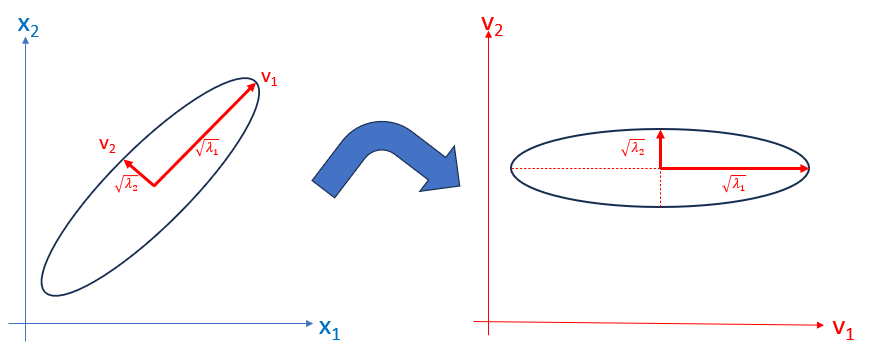
\includegraphics[width=1\textwidth,height=\textheight]{images/pca-rotation.png}

}

\caption{\label{fig-pca-rotation}Geometry of PCA as a rotation from data
space to principal component space, defined by the eigenvectors v1 and
v2 of a covariance matrix}

\end{figure}

\hypertarget{finding-principal-components}{%
\subsection{Finding principal
components}\label{finding-principal-components}}

In R, principal components analysis is most easily carried out using
\texttt{stats::prcomp()} or \texttt{stats::princomp()} or similar
functions in other packages such as \texttt{FactomineR::PCA()}. The
\textbf{FactoMineR} package
(\protect\hyperlink{ref-Husson-etal-2017}{Husson et al., 2017},
\protect\hyperlink{ref-R-FactoMineR}{2023}) has extensive capabilities
for exploratory analysis of multivariate data (PCA, correspondence
analysis, cluster analysis).

A particular strength of FactoMineR for PCA is that it allows the
inclusion of \emph{supplementary variables} (which can be categorical or
quantitative) and \emph{supplementary points} for individuals. These are
not used in the analysis, but are projected into the plots to facilitate
interpretation. For example, in the analysis of the \texttt{crime} data
described below, it would be useful to have measures of other
characteristics of the U.S. states, such as poverty and average level of
education (Section~\ref{sec-supp-vars}).

Unfortunately, although all of these functions perform similar
calculations, the options for analysis and the details of the result
they return differ.

The important options for analysis include:

\begin{itemize}
\tightlist
\item
  whether or not the data variables are \textbf{centered}, to a mean of
  \(\bar{x}_j =0\)
\item
  whether or not the data variables are \textbf{scaled}, to a variance
  of \(\text{Var}(x_j) =1\).
\end{itemize}

It nearly always makes sense to center the variables. The choice of
scaling determines whether the correlation matrix is analyzed, so that
each variable contributes equally to the total variance that is to be
accounted for versus analysis of the covariance matrix, where each
variable contributes its own variance to the total. Analysis of the
covariance matrix makes little sense when the variables are measured on
different scales.\footnote{For example, if two variables in the analysis
  are height and weight, changing the unit of height from inches to
  centimeters would multiply its' variance by \(2.54^2\); changing
  weight from pounds to kilograms would divide its' variance by
  \(2.2^2\).}

\hypertarget{example-crime-data}{%
\subsubsection*{Example: Crime data}\label{example-crime-data}}
\addcontentsline{toc}{subsubsection}{Example: Crime data}

The dataset \texttt{crime}, analysed in Section~\ref{sec-corrgram},
showed all positive correlations among the rates of various crimes in
the corrgram, Figure~\ref{fig-crime-corrplot}. What can we see from a
principal components analysis? Is it possible that a few dimensions can
account for most of the juice in this data?

In this example, you can easily find the PCA solution using
\texttt{prcomp()} in a single line in base-R. You need to specify the
numeric variables to analyze by their columns in the data frame. The
most important option here is \texttt{scale.\ =\ TRUE} \ldots{}

\begin{Shaded}
\begin{Highlighting}[]
\FunctionTok{data}\NormalTok{(crime, }\AttributeTok{package =} \StringTok{"ggbiplot"}\NormalTok{)}
\NormalTok{crime.pca }\OtherTok{\textless{}{-}} \FunctionTok{prcomp}\NormalTok{(crime[, }\DecValTok{2}\SpecialCharTok{:}\DecValTok{8}\NormalTok{], }\AttributeTok{scale. =} \ConstantTok{TRUE}\NormalTok{)}
\end{Highlighting}
\end{Shaded}

The tidy equivalent is more verbose, but also more expressive about what
is being done. It selects the variables to analyze by a function,
\texttt{is.numeric()} applied to each of the columns and feeds the
result to \texttt{prcomp()}.

\begin{Shaded}
\begin{Highlighting}[]
\NormalTok{crime.pca }\OtherTok{\textless{}{-}} 
\NormalTok{  crime }\SpecialCharTok{|\textgreater{}} 
\NormalTok{  dplyr}\SpecialCharTok{::}\FunctionTok{select}\NormalTok{(}\FunctionTok{where}\NormalTok{(is.numeric)) }\SpecialCharTok{|\textgreater{}}
  \FunctionTok{prcomp}\NormalTok{(}\AttributeTok{scale. =} \ConstantTok{TRUE}\NormalTok{)}
\end{Highlighting}
\end{Shaded}

As is typical with models in R, the result, \texttt{crime.pca} of
\texttt{prcomp()} is an object of class \texttt{"prcomp"}, a list of
components, and there are a variety of methods for \texttt{"prcomp"}
objects. Among the simplest is \texttt{summary()}, which gives the
contributions of each component to the total variance in the dataset.

\begin{Shaded}
\begin{Highlighting}[]
\FunctionTok{summary}\NormalTok{(crime.pca) }\SpecialCharTok{|\textgreater{}} \FunctionTok{print}\NormalTok{(}\AttributeTok{digits=}\DecValTok{2}\NormalTok{)}
\CommentTok{\#\textgreater{} Importance of components:}
\CommentTok{\#\textgreater{}                         PC1  PC2  PC3   PC4   PC5   PC6   PC7}
\CommentTok{\#\textgreater{} Standard deviation     2.03 1.11 0.85 0.563 0.508 0.471 0.352}
\CommentTok{\#\textgreater{} Proportion of Variance 0.59 0.18 0.10 0.045 0.037 0.032 0.018}
\CommentTok{\#\textgreater{} Cumulative Proportion  0.59 0.76 0.87 0.914 0.951 0.982 1.000}
\end{Highlighting}
\end{Shaded}

The object, \texttt{crime.pca} returned by \texttt{prcomp()} is a list
of the following the following elements:

\begin{Shaded}
\begin{Highlighting}[]
\FunctionTok{names}\NormalTok{(crime.pca)}
\CommentTok{\#\textgreater{} [1] "sdev"     "rotation" "center"   "scale"    "x"}
\end{Highlighting}
\end{Shaded}

Of these, for \(n\) observations and \(p\) variables,

\begin{itemize}
\tightlist
\item
  \texttt{sdev} is the length \(p\) vector of the standard deviations of
  the principal components (i.e., the square roots \(\sqrt{\lambda_i}\)
  of the eigenvalues of the covariance/correlation matrix). When the
  variables are standardized, the sum of squares of the eigenvalues is
  equal to \(p\).
\item
  \texttt{rotation} is the \(p \times p\) matrix of weights or
  \textbf{loadings} of the variables on the components; the columns are
  the eigenvectors of the covariance or correlation matrix of the data;
\item
  \texttt{x} is the \(n \times p\) matrix of \textbf{scores} for the
  observations on the components, the result of multiplying (rotating)
  the data matrix by the loadings. These are uncorrelated, so
  \texttt{cov(x)} is a \(p \times p\) diagonal matrix whose diagonal
  elements are the eigenvalues \(\lambda_i\) = \texttt{sdev\^{}2}.
\end{itemize}

\hypertarget{visualizing-variance-proportions-screeplots}{%
\subsection{Visualizing variance proportions:
screeplots}\label{visualizing-variance-proportions-screeplots}}

For a high-D dataset, such as the crime data in seven dimensions, a
natural question is how much of the variation in the data can be
captured in 1D, 2D, 3D, \ldots{} summaries and views. This is answered
by considering the proportions of variance accounted by each of the
dimensions, or their cumulative values. The components returned by
various PCA methods have (confusingly) different names, so
\texttt{broom::tidy()} provides methods to unify extraction of these
values.

\begin{Shaded}
\begin{Highlighting}[]
\NormalTok{(crime.eig }\OtherTok{\textless{}{-}}\NormalTok{ crime.pca }\SpecialCharTok{|\textgreater{}} 
\NormalTok{  broom}\SpecialCharTok{::}\FunctionTok{tidy}\NormalTok{(}\AttributeTok{matrix =} \StringTok{"eigenvalues"}\NormalTok{))}
\CommentTok{\#\textgreater{} \# A tibble: 7 x 4}
\CommentTok{\#\textgreater{}      PC std.dev percent cumulative}
\CommentTok{\#\textgreater{}   \textless{}dbl\textgreater{}   \textless{}dbl\textgreater{}   \textless{}dbl\textgreater{}      \textless{}dbl\textgreater{}}
\CommentTok{\#\textgreater{} 1     1   2.03   0.588       0.588}
\CommentTok{\#\textgreater{} 2     2   1.11   0.177       0.765}
\CommentTok{\#\textgreater{} 3     3   0.852  0.104       0.868}
\CommentTok{\#\textgreater{} 4     4   0.563  0.0452      0.914}
\CommentTok{\#\textgreater{} 5     5   0.508  0.0368      0.951}
\CommentTok{\#\textgreater{} 6     6   0.471  0.0317      0.982}
\CommentTok{\#\textgreater{} 7     7   0.352  0.0177      1}
\end{Highlighting}
\end{Shaded}

Then, a simple visualization is a plot of the proportion of variance for
each component (or cumulative proportion) against the component number,
usually called a \textbf{screeplot}. The idea, introduced by Cattell
(\protect\hyperlink{ref-Cattell1966}{1966}), is that after the largest,
dominant components, the remainder should resemble the rubble, or scree
formed by rocks falling from a cliff.

From this plot, imagine drawing a straight line through the plotted
eigenvalues, starting with the largest one. The typical rough guidance
is that the last point to fall on this line represents the last
component to extract, the idea being that beyond this, the amount of
additional variance explained is non-meaningful. Another rule of thumb
is to choose the number of components to extract a desired proportion of
total variance, usually in the range of 80 - 90\%.

\texttt{stats::plot(crime.pca)} would give a bar plot of the variances
of the components, however \texttt{ggbiplot::ggscreeplot()} gives nicer
and more flexible displays as shown in
Figure~\ref{fig-crime-ggscreeplot}.

\begin{Shaded}
\begin{Highlighting}[]
\NormalTok{p1 }\OtherTok{\textless{}{-}} \FunctionTok{ggscreeplot}\NormalTok{(crime.pca) }\SpecialCharTok{+}
  \FunctionTok{stat\_smooth}\NormalTok{(}\AttributeTok{data =}\NormalTok{ crime.eig }\SpecialCharTok{|\textgreater{}} \FunctionTok{filter}\NormalTok{(PC}\SpecialCharTok{\textgreater{}=}\DecValTok{4}\NormalTok{), }
              \FunctionTok{aes}\NormalTok{(}\AttributeTok{x=}\NormalTok{PC, }\AttributeTok{y=}\NormalTok{percent), }\AttributeTok{method =} \StringTok{"lm"}\NormalTok{, }
              \AttributeTok{se =} \ConstantTok{FALSE}\NormalTok{,}
              \AttributeTok{fullrange =} \ConstantTok{TRUE}\NormalTok{) }\SpecialCharTok{+}
  \FunctionTok{theme\_bw}\NormalTok{(}\AttributeTok{base\_size =} \DecValTok{14}\NormalTok{)}

\NormalTok{p2 }\OtherTok{\textless{}{-}} \FunctionTok{ggscreeplot}\NormalTok{(crime.pca, }\AttributeTok{type =} \StringTok{"cev"}\NormalTok{) }\SpecialCharTok{+}
  \FunctionTok{geom\_hline}\NormalTok{(}\AttributeTok{yintercept =} \FunctionTok{c}\NormalTok{(}\FloatTok{0.8}\NormalTok{, }\FloatTok{0.9}\NormalTok{), }\AttributeTok{color =} \StringTok{"blue"}\NormalTok{) }\SpecialCharTok{+}
  \FunctionTok{theme\_bw}\NormalTok{(}\AttributeTok{base\_size =} \DecValTok{14}\NormalTok{)}

\NormalTok{p1 }\SpecialCharTok{+}\NormalTok{ p2}
\end{Highlighting}
\end{Shaded}

\begin{figure}[H]

{\centering 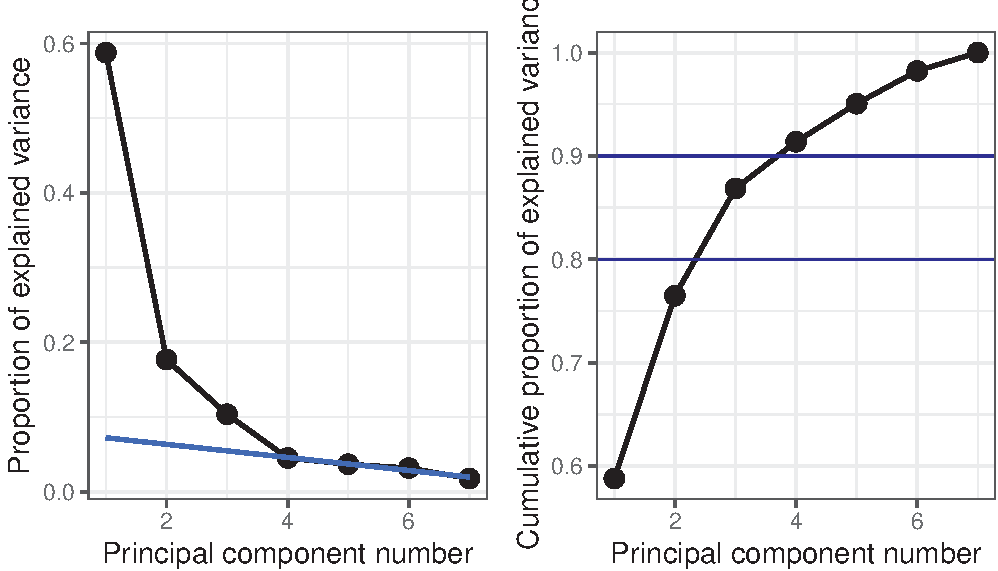
\includegraphics[width=1\textwidth,height=\textheight]{figs/ch04/fig-crime-ggscreeplot-1.pdf}

}

\caption{\label{fig-crime-ggscreeplot}Screeplots for the PCA of the
crime data. The left panel shows the traditional version, plotting
variance proportions against component number, with linear guideline for
the scree rule of thumb. The right panel plots cumulative proportions,
showing cutoffs of 80\%, 90\%.}

\end{figure}

From this we might conclude that four components are necessary to
satisfy the scree criterion or to account for 90\% of the total
variation in these crime statistics. However two components, giving
76.5\%, might be enough juice to tell a reasonable story.

\hypertarget{visualizing-pca-scores-and-variable-vectors}{%
\subsection{Visualizing PCA scores and variable
vectors}\label{visualizing-pca-scores-and-variable-vectors}}

To see and attempt to understand PCA results, it is useful to plot both
the scores for the observations on a few of the largest components and
also the loadings or variable vectors that give the weights for the
variables in determining the principal components.

In Section~\ref{sec-biplot} I discuss the biplot technique that plots
both in a single display. However, I do this directly here, using tidy
processing to explain what is going on in PCA and in these graphical
displays.

\hypertarget{scores}{%
\subsubsection*{Scores}\label{scores}}
\addcontentsline{toc}{subsubsection}{Scores}

The (uncorrelated) principal component scores can be extracted as
\texttt{crime.pca\$x} or using \texttt{purrr::pluck("x")}. As noted
above, these are uncorrelated and have variances equal to the
eigenvalues of the correlation matrix.

\begin{Shaded}
\begin{Highlighting}[]
\NormalTok{scores }\OtherTok{\textless{}{-}}\NormalTok{ crime.pca }\SpecialCharTok{|\textgreater{}}\NormalTok{ purrr}\SpecialCharTok{::}\FunctionTok{pluck}\NormalTok{(}\StringTok{"x"}\NormalTok{) }
\FunctionTok{cov}\NormalTok{(scores) }\SpecialCharTok{|\textgreater{}} \FunctionTok{zapsmall}\NormalTok{()}
\CommentTok{\#\textgreater{}      PC1  PC2  PC3  PC4  PC5  PC6  PC7}
\CommentTok{\#\textgreater{} PC1 4.11 0.00 0.00 0.00 0.00 0.00 0.00}
\CommentTok{\#\textgreater{} PC2 0.00 1.24 0.00 0.00 0.00 0.00 0.00}
\CommentTok{\#\textgreater{} PC3 0.00 0.00 0.73 0.00 0.00 0.00 0.00}
\CommentTok{\#\textgreater{} PC4 0.00 0.00 0.00 0.32 0.00 0.00 0.00}
\CommentTok{\#\textgreater{} PC5 0.00 0.00 0.00 0.00 0.26 0.00 0.00}
\CommentTok{\#\textgreater{} PC6 0.00 0.00 0.00 0.00 0.00 0.22 0.00}
\CommentTok{\#\textgreater{} PC7 0.00 0.00 0.00 0.00 0.00 0.00 0.12}
\end{Highlighting}
\end{Shaded}

For plotting, it is more convenient to use \texttt{broom::augment()}
which extracts the scores (named \texttt{.fittedPC*}) and appends these
to the variables in the dataset.

\begin{Shaded}
\begin{Highlighting}[]
\NormalTok{crime.pca }\SpecialCharTok{|\textgreater{}}
\NormalTok{  broom}\SpecialCharTok{::}\FunctionTok{augment}\NormalTok{(crime) }\SpecialCharTok{|\textgreater{}} \FunctionTok{head}\NormalTok{()}
\CommentTok{\#\textgreater{} \# A tibble: 6 x 18}
\CommentTok{\#\textgreater{}   .rownames state      murder  rape robbery assault burglary larceny}
\CommentTok{\#\textgreater{}   \textless{}chr\textgreater{}     \textless{}chr\textgreater{}       \textless{}dbl\textgreater{} \textless{}dbl\textgreater{}   \textless{}dbl\textgreater{}   \textless{}dbl\textgreater{}    \textless{}dbl\textgreater{}   \textless{}dbl\textgreater{}}
\CommentTok{\#\textgreater{} 1 1         Alabama      14.2  25.2    96.8    278.    1136.   1882.}
\CommentTok{\#\textgreater{} 2 2         Alaska       10.8  51.6    96.8    284     1332.   3370.}
\CommentTok{\#\textgreater{} 3 3         Arizona       9.5  34.2   138.     312.    2346.   4467.}
\CommentTok{\#\textgreater{} 4 4         Arkansas      8.8  27.6    83.2    203.     973.   1862.}
\CommentTok{\#\textgreater{} 5 5         California   11.5  49.4   287      358     2139.   3500.}
\CommentTok{\#\textgreater{} 6 6         Colorado      6.3  42     171.     293.    1935.   3903.}
\CommentTok{\#\textgreater{} \# i 10 more variables: auto \textless{}dbl\textgreater{}, st \textless{}chr\textgreater{}, region \textless{}fct\textgreater{},}
\CommentTok{\#\textgreater{} \#   .fittedPC1 \textless{}dbl\textgreater{}, .fittedPC2 \textless{}dbl\textgreater{}, .fittedPC3 \textless{}dbl\textgreater{},}
\CommentTok{\#\textgreater{} \#   .fittedPC4 \textless{}dbl\textgreater{}, .fittedPC5 \textless{}dbl\textgreater{}, .fittedPC6 \textless{}dbl\textgreater{},}
\CommentTok{\#\textgreater{} \#   .fittedPC7 \textless{}dbl\textgreater{}}
\end{Highlighting}
\end{Shaded}

Then, we can use \texttt{ggplot()} to plot any pair of components. To
aid interpretation, I label the points by their state abbreviation and
color them by \texttt{region} of the U.S.. A geometric interpretation of
the plot requires an aspect ratio of 1.0 (via \texttt{coord\_fixed()})
so that a unit distance on the horizontal axis is the same length as a
unit distance on the vertical. To demonstrate that the components are
uncorrelated, I also added their data ellipse.

\begin{Shaded}
\begin{Highlighting}[]
\NormalTok{crime.pca }\SpecialCharTok{|\textgreater{}}
\NormalTok{  broom}\SpecialCharTok{::}\FunctionTok{augment}\NormalTok{(crime) }\SpecialCharTok{|\textgreater{}} \CommentTok{\# add original dataset back in}
  \FunctionTok{ggplot}\NormalTok{(}\FunctionTok{aes}\NormalTok{(.fittedPC1, .fittedPC2, }\AttributeTok{color =}\NormalTok{ region)) }\SpecialCharTok{+} 
  \FunctionTok{geom\_hline}\NormalTok{(}\AttributeTok{yintercept =} \DecValTok{0}\NormalTok{) }\SpecialCharTok{+}
  \FunctionTok{geom\_vline}\NormalTok{(}\AttributeTok{xintercept =} \DecValTok{0}\NormalTok{) }\SpecialCharTok{+}
  \FunctionTok{geom\_point}\NormalTok{(}\AttributeTok{size =} \FloatTok{1.5}\NormalTok{) }\SpecialCharTok{+}
  \FunctionTok{geom\_text}\NormalTok{(}\FunctionTok{aes}\NormalTok{(}\AttributeTok{label =}\NormalTok{ st), }\AttributeTok{nudge\_x =} \FloatTok{0.2}\NormalTok{) }\SpecialCharTok{+}
  \FunctionTok{stat\_ellipse}\NormalTok{(}\AttributeTok{color =} \StringTok{"grey"}\NormalTok{) }\SpecialCharTok{+}
  \FunctionTok{coord\_fixed}\NormalTok{() }\SpecialCharTok{+}
  \FunctionTok{labs}\NormalTok{(}\AttributeTok{x =} \StringTok{"PC Dimension 1"}\NormalTok{, }\AttributeTok{y =} \StringTok{"PC Dimnension 2"}\NormalTok{) }\SpecialCharTok{+}
  \FunctionTok{theme\_minimal}\NormalTok{(}\AttributeTok{base\_size =} \DecValTok{14}\NormalTok{) }\SpecialCharTok{+}
  \FunctionTok{theme}\NormalTok{(}\AttributeTok{legend.position =} \StringTok{"top"}\NormalTok{) }
\end{Highlighting}
\end{Shaded}

\begin{figure}[H]

{\centering 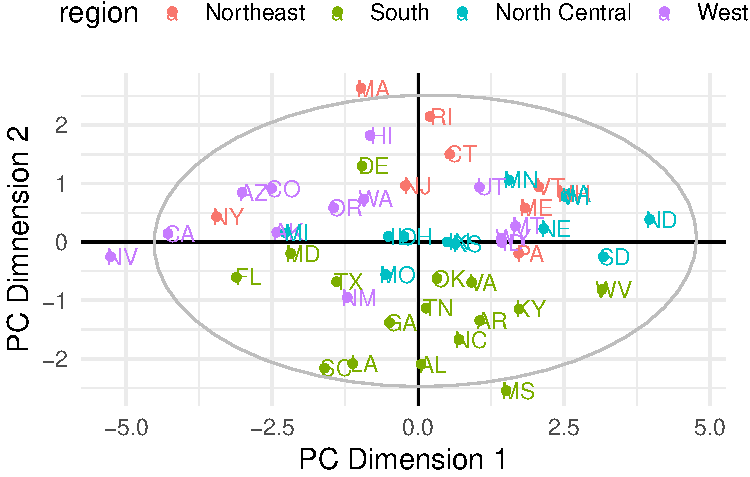
\includegraphics[width=1\textwidth,height=\textheight]{figs/ch04/fig-crime-scores-plot12-1.pdf}

}

\caption{\label{fig-crime-scores-plot12}Plot of component scores on the
first two principal components for the \texttt{crime} data. States are
colored by \texttt{region}.}

\end{figure}

To interpret such plots, it is useful consider the observations that are
a high and low on each of the axes as well as other information, such as
region here, and ask how these differ on the crime statistics. The first
component, PC1, contrasts Nevada and California with North Dakota, South
Dakota and West Virginia. The second component has most of the southern
states on the low end and Massachusetts, Rhode Island and Hawaii on the
high end. However, interpretation is easier when we also consider how
the various crimes contribute to these dimensions.

When, as here, there are more than two components that seem important in
the scree plot, we could obviously go further and plot other pairs.

\hypertarget{variable-vectors}{%
\subsubsection*{Variable vectors}\label{variable-vectors}}
\addcontentsline{toc}{subsubsection}{Variable vectors}

You can extract the variable loadings using either
\texttt{crime.pca\$rotation} or \texttt{purrr::pluck("rotation")},
similar to what I did with the scores.

\begin{Shaded}
\begin{Highlighting}[]
\NormalTok{crime.pca }\SpecialCharTok{|\textgreater{}}\NormalTok{ purrr}\SpecialCharTok{::}\FunctionTok{pluck}\NormalTok{(}\StringTok{"rotation"}\NormalTok{)}
\CommentTok{\#\textgreater{}             PC1     PC2     PC3     PC4     PC5     PC6     PC7}
\CommentTok{\#\textgreater{} murder   {-}0.300 {-}0.6292  0.1782 {-}0.2321  0.5381  0.2591  0.2676}
\CommentTok{\#\textgreater{} rape     {-}0.432 {-}0.1694 {-}0.2442  0.0622  0.1885 {-}0.7733 {-}0.2965}
\CommentTok{\#\textgreater{} robbery  {-}0.397  0.0422  0.4959 {-}0.5580 {-}0.5200 {-}0.1144 {-}0.0039}
\CommentTok{\#\textgreater{} assault  {-}0.397 {-}0.3435 {-}0.0695  0.6298 {-}0.5067  0.1724  0.1917}
\CommentTok{\#\textgreater{} burglary {-}0.440  0.2033 {-}0.2099 {-}0.0576  0.1010  0.5360 {-}0.6481}
\CommentTok{\#\textgreater{} larceny  {-}0.357  0.4023 {-}0.5392 {-}0.2349  0.0301  0.0394  0.6017}
\CommentTok{\#\textgreater{} auto     {-}0.295  0.5024  0.5684  0.4192  0.3698 {-}0.0573  0.1470}
\end{Highlighting}
\end{Shaded}

But note something important in this output: All of the weights for the
first component are negative. In PCA, the directions of the eigenvectors
are completely arbitrary, in the sense that the vector \(-\mathbf{v}_i\)
gives the same linear combination as \(\mathbf{v}_i\), but with its'
sign reversed. For interpretation, it is useful (and usually
recommended) to reflect the loadings to a positive orientation by
multiplying them by -1.

To reflect the PCA loadings and get them into a convenient format for
plotting with \texttt{ggplot()}, it is necessary to do a bit of
processing, including making the \texttt{row.names()} into an explicit
variable for the purpose of labeling.

\textbf{TODO}: Should this be a callout-warning or a footnote??

\begin{tcolorbox}[enhanced jigsaw, colback=white, rightrule=.15mm, left=2mm, arc=.35mm, colframe=quarto-callout-warning-color-frame, toptitle=1mm, breakable, leftrule=.75mm, opacityback=0, bottomtitle=1mm, colbacktitle=quarto-callout-warning-color!10!white, opacitybacktitle=0.6, titlerule=0mm, toprule=.15mm, title=\textcolor{quarto-callout-warning-color}{\faExclamationTriangle}\hspace{0.5em}{\texttt{rownames} in R}, bottomrule=.15mm, coltitle=black]

R software evolved over many years, particularly in conventions for
labeling cases in printed output and graphics. In base-R, the convention
was that the \texttt{row.names()} of a matrix or data.frame served as
observation labels in all printed output and plots, with a default to
use numbers \texttt{1:n} if there were no rownames. In \texttt{ggplot2}
and the \texttt{tidyverse} framework, the decision was made that
observation labels had to be an \textbf{explicit} variable in a ``tidy''
dataset, so it could be used as a variable in constructs like
\texttt{geom\_text(aes(label\ =\ label))} as in this example. This
change often requires extra steps in software that uses the rownames
convention.

\end{tcolorbox}

\begin{Shaded}
\begin{Highlighting}[]
\NormalTok{vectors }\OtherTok{\textless{}{-}}\NormalTok{ crime.pca }\SpecialCharTok{|\textgreater{}} 
\NormalTok{  purrr}\SpecialCharTok{::}\FunctionTok{pluck}\NormalTok{(}\StringTok{"rotation"}\NormalTok{) }\SpecialCharTok{|\textgreater{}}
  \FunctionTok{as.data.frame}\NormalTok{() }\SpecialCharTok{|\textgreater{}}
  \FunctionTok{mutate}\NormalTok{(}\AttributeTok{PC1 =} \SpecialCharTok{{-}}\DecValTok{1} \SpecialCharTok{*}\NormalTok{ PC1, }\AttributeTok{PC2 =} \SpecialCharTok{{-}}\DecValTok{1} \SpecialCharTok{*}\NormalTok{ PC2) }\SpecialCharTok{|\textgreater{}}      \CommentTok{\# reflect axes}
\NormalTok{  tibble}\SpecialCharTok{::}\FunctionTok{rownames\_to\_column}\NormalTok{(}\AttributeTok{var =} \StringTok{"label"}\NormalTok{) }

\NormalTok{vectors[, }\DecValTok{1}\SpecialCharTok{:}\DecValTok{3}\NormalTok{]}
\CommentTok{\#\textgreater{}      label   PC1     PC2}
\CommentTok{\#\textgreater{} 1   murder 0.300  0.6292}
\CommentTok{\#\textgreater{} 2     rape 0.432  0.1694}
\CommentTok{\#\textgreater{} 3  robbery 0.397 {-}0.0422}
\CommentTok{\#\textgreater{} 4  assault 0.397  0.3435}
\CommentTok{\#\textgreater{} 5 burglary 0.440 {-}0.2033}
\CommentTok{\#\textgreater{} 6  larceny 0.357 {-}0.4023}
\CommentTok{\#\textgreater{} 7     auto 0.295 {-}0.5024}
\end{Highlighting}
\end{Shaded}

Then, I plot these using \texttt{geom\_segment()}, taking some care to
use arrows from the origin with a nice shape and add
\texttt{geom\_text()} labels for the variables positioned slightly to
the right. Again, \texttt{coord\_fixed()} ensures equal scales for the
axes, which is important because we want to interpret the angles between
the variable vectors and the PCA coordinate axes.

\begin{Shaded}
\begin{Highlighting}[]
\NormalTok{arrow\_style }\OtherTok{\textless{}{-}} \FunctionTok{arrow}\NormalTok{(}
  \AttributeTok{angle =} \DecValTok{20}\NormalTok{, }\AttributeTok{ends =} \StringTok{"first"}\NormalTok{, }\AttributeTok{type =} \StringTok{"closed"}\NormalTok{, }
  \AttributeTok{length =}\NormalTok{ grid}\SpecialCharTok{::}\FunctionTok{unit}\NormalTok{(}\DecValTok{8}\NormalTok{, }\StringTok{"pt"}\NormalTok{)}
\NormalTok{)}

\NormalTok{vectors }\SpecialCharTok{|\textgreater{}}
  \FunctionTok{ggplot}\NormalTok{(}\FunctionTok{aes}\NormalTok{(PC1, PC2)) }\SpecialCharTok{+}
  \FunctionTok{geom\_hline}\NormalTok{(}\AttributeTok{yintercept =} \DecValTok{0}\NormalTok{) }\SpecialCharTok{+}
  \FunctionTok{geom\_vline}\NormalTok{(}\AttributeTok{xintercept =} \DecValTok{0}\NormalTok{) }\SpecialCharTok{+}
  \FunctionTok{geom\_segment}\NormalTok{(}\AttributeTok{xend =} \DecValTok{0}\NormalTok{, }\AttributeTok{yend =} \DecValTok{0}\NormalTok{, }
               \AttributeTok{linewidth =} \DecValTok{1}\NormalTok{, }
               \AttributeTok{arrow =}\NormalTok{ arrow\_style,}
               \AttributeTok{color =} \StringTok{"brown"}\NormalTok{) }\SpecialCharTok{+}
  \FunctionTok{geom\_text}\NormalTok{(}\FunctionTok{aes}\NormalTok{(}\AttributeTok{label =}\NormalTok{ label), }
            \AttributeTok{size =} \DecValTok{5}\NormalTok{,}
            \AttributeTok{hjust =} \StringTok{"outward"}\NormalTok{,}
            \AttributeTok{nudge\_x =} \FloatTok{0.05}\NormalTok{, }
            \AttributeTok{color =} \StringTok{"brown"}\NormalTok{) }\SpecialCharTok{+}
  \FunctionTok{xlim}\NormalTok{(}\SpecialCharTok{{-}}\FloatTok{0.4}\NormalTok{, }\FloatTok{0.9}\NormalTok{) }\SpecialCharTok{+} 
  \FunctionTok{ylim}\NormalTok{(}\SpecialCharTok{{-}}\FloatTok{0.8}\NormalTok{, }\FloatTok{0.8}\NormalTok{) }\SpecialCharTok{+}
  \FunctionTok{coord\_fixed}\NormalTok{() }\SpecialCharTok{+} 
  \FunctionTok{theme\_minimal}\NormalTok{(}\AttributeTok{base\_size =} \DecValTok{14}\NormalTok{)}
\end{Highlighting}
\end{Shaded}

\begin{figure}[H]

{\centering 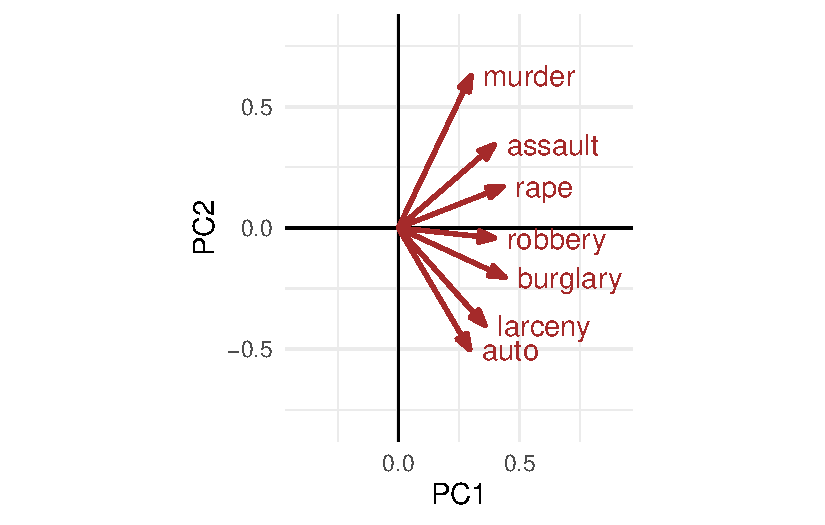
\includegraphics[width=0.8\textwidth,height=\textheight]{figs/ch04/fig-crime-vectors-1.pdf}

}

\caption{\label{fig-crime-vectors}Plot of component loadings the first
two principal components for the \texttt{crime} data. These are
interpreted as the contributions of the variables to the components.}

\end{figure}

What is shown in Figure~\ref{fig-crime-vectors} has the following
interpretations:

\begin{enumerate}
\def\labelenumi{(\arabic{enumi})}
\item
  the lengths of the variable vectors,
  \(||\mathbf{v}_i|| = \sqrt{\Sigma_{j = 1}^{j=2} \; v_{ij}^2}\) give
  the proportion of variance of each variable accounted for in a
  two-dimensional display.
\item
  the value, \(v_{ij}\), of the vector for variable \(\mathbf{x}_i\) on
  component \(j\) gives the correlation of that variable with the
  \(j\)th principal component.
\item
  the cosine of the angle between two variable vectors, \(\mathbf{v}_i\)
  and \(\mathbf{v}_j\) gives the approximation of the correlation
  between \(\mathbf{x}_i\) and \(\mathbf{x}_j\) that is shown in this
  space. This means that two variable vectors that point in the same
  direction are highly correlated, while variable vectors at right
  angles are approximately uncorrelated.
\end{enumerate}

To illustrate point (1), the following indicates that almost 70\% of the
variance of \texttt{murder} is represented in the the 2D plot shown in
Figure~\ref{fig-crime-scores-plot12}, but only 40\% of the variance of
\texttt{robbery} is captured.

\begin{Shaded}
\begin{Highlighting}[]
\NormalTok{vectors }\SpecialCharTok{|\textgreater{}} \FunctionTok{select}\NormalTok{(label, PC1, PC2) }\SpecialCharTok{|\textgreater{}} 
  \FunctionTok{mutate}\NormalTok{(}\AttributeTok{length =} \FunctionTok{sqrt}\NormalTok{(PC1}\SpecialCharTok{\^{}}\DecValTok{2} \SpecialCharTok{+}\NormalTok{ PC2}\SpecialCharTok{\^{}}\DecValTok{2}\NormalTok{))}
\CommentTok{\#\textgreater{}      label   PC1     PC2 length}
\CommentTok{\#\textgreater{} 1   murder 0.300  0.6292  0.697}
\CommentTok{\#\textgreater{} 2     rape 0.432  0.1694  0.464}
\CommentTok{\#\textgreater{} 3  robbery 0.397 {-}0.0422  0.399}
\CommentTok{\#\textgreater{} 4  assault 0.397  0.3435  0.525}
\CommentTok{\#\textgreater{} 5 burglary 0.440 {-}0.2033  0.485}
\CommentTok{\#\textgreater{} 6  larceny 0.357 {-}0.4023  0.538}
\CommentTok{\#\textgreater{} 7     auto 0.295 {-}0.5024  0.583}
\end{Highlighting}
\end{Shaded}

\hypertarget{sec-biplot}{%
\section{Biplots}\label{sec-biplot}}

The biplot is a simple and powerful idea that came from the recognition
that you can overlay a plot of observation scores in a principal
components analysis with the information of the variable loadings
(weights) to give a simultaneous display that is easy to interpret. In
this sense, a biplot is generalization of a scatterplot, projecting from
data space to PCA space, where the observations are shown by points, as
in the plots of component scores in
Figure~\ref{fig-crime-scores-plot12}, but with the variables also shown
by vectors (or scaled linear axes aligned with those vectors).

The idea of the biplot was introduced by Ruben Gabriel
(\protect\hyperlink{ref-Gabriel:71}{1971},
\protect\hyperlink{ref-Gabriel:81}{1981}) and later expanded in scope by
Gower \& Hand (\protect\hyperlink{ref-GowerHand:96}{1996}). The book by
Greenacre (\protect\hyperlink{ref-Greenacre:2010:biplots}{2010}) gives a
practical overview of the many variety of biplots and Gower et al.
(\protect\hyperlink{ref-Gower-etal:2011}{2011}) provide a full treatment
\ldots{}

Biplot methodolgy is far more general than I cover here. Categorical
variables can be incorporated in PCA using category level points.
Two-way frequency tables of categorical variables can be analysed using
\emph{correspondence analysis}, which is similar to PCA, but designed to
account for the maximum amount of the \(\chi^2\) statistic for
association; \emph{multiple correspondence analysis} extends this to
method to multi-way tables
(\protect\hyperlink{ref-FriendlyMeyer:2016:DDAR}{Friendly \& Meyer,
2016}; \protect\hyperlink{ref-Greenacre:84}{Greenacre, 1984}).

\hypertarget{constructing-a-biplot}{%
\subsection{Constructing a biplot}\label{constructing-a-biplot}}

The biplot is constructed by using the singular value decomposition
(SVD) to obtain a low-rank approximation to the data matrix
\(\mathbf{X}_{n \times p}\) (centered, and optionally scaled to unit
variances) whose \(n\) rows are the observations and whose \(p\) columns
are the variables.

\begin{figure}

{\centering \includegraphics[width=0.8\textwidth,height=\textheight]{images/SVD-eqn.jpg}

}

\caption{\label{fig-svd-diagram}The singular value decomposition
expresses a data matrix \textbf{X} as the product of a matrix \textbf{U}
of observation scores, a diagonal matrix \textbf{Lambda} of singular
values and a matrix \textbf{V} of variable weights. \textbf{TODO}:
Re-draw to fix notation.}

\end{figure}

Using the SVD, the matrix \(\mathbf{X}\), of rank \(r \le p\) can be
expressed \emph{exactly} as:
\begin{equation}\protect\hypertarget{eq-svd1}{}{
\mathbf{X} = \mathbf{U} \mathbf{\Lambda} \mathbf{V}'
                 = \sum_i^r \lambda_i \mathbf{u}_i \mathbf{v}_i' \; ,
}\label{eq-svd1}\end{equation}

where

\begin{itemize}
\tightlist
\item
  \(\mathbf{U}\) is an \(n \times r\) orthonormal matrix of uncorrelated
  observation scores; these are also the eigenvectors of
  \(\mathbf{X} \mathbf{X}'\),
\item
  \(\mathbf{\Lambda}\) is an \(r \times r\) diagonal matrix of singular
  values, \(\lambda_1 \ge \lambda_2 \ge \cdots \lambda_r\), which are
  also the square roots of the eigenvalues of
  \(\mathbf{X} \mathbf{X}'\).
\item
  \(\mathbf{V}\) is an \(r \times p\) orthonormal matrix of variable
  weights and also the eigenvectors of \(\mathbf{X}' \mathbf{X}\).
\end{itemize}

Then, a rank 2 (or 3) PCA approximation \(\widehat{\mathbf{X}}\) to the
data matrix used in the biplot can be obtained from the first 2 (or 3)
singular values \(\lambda_i\) and the corresponding
\(\mathbf{u}_i, \mathbf{v}_i\) as:

\[
\mathbf{X} \approx \widehat{\mathbf{X}} = \lambda_1 \mathbf{u}_1 \mathbf{v}_1' + \lambda_2 \mathbf{u}_2 \mathbf{v}_2' \; .
\]

The variance of \(\mathbf{X}\) accounted for by each term is
\(\lambda_i^2\).

A biplot is then obtained by overlaying two scatterplots that share a
common set of axes and have a between-set scalar product interpretation.
Typically, the observations (rows of \(\mathbf{X}\)) are represented as
points and the variables (columns of \(\mathbf{X}\)) are represented as
vectors from the origin.

The \code{scale} factor, \(\alpha\) allows the variances of the
components to be apportioned between the row points and column vectors,
with different interpretations, by representing the approximation
\(\widehat{\mathbf{X}}\) as the product of two matrices,

\[
\widehat{\mathbf{X}} = (\mathbf{U} \mathbf{\Lambda}^\alpha) (\mathbf{\Lambda}^{1-\alpha} \mathbf{V}') = \mathbf{A} \mathbf{B}'
\] This notation uses a little math trick involving a power,
\(0 \le \alpha \le 1\): When \(\alpha = 1\),
\(\mathbf{\Lambda}^\alpha = \mathbf{\Lambda}^1 =\mathbf{\Lambda}\), and
\(\mathbf{\Lambda}^{1-\alpha} = \mathbf{\Lambda}^0 =\mathbf{I}\).
\(\alpha = 1/2\) gives the diagonal matrix \(\mathbf{\Lambda}^{1/2}\)
whose elements are the square roots of the singular values.

The choice \(\alpha = 1\) assigns the singular values totally to the
left factor; then, the angle between two variable vectors, reflecting
the inner product \(\mathbf{x}_j^T, \mathbf{x}_{j'}\) approximates their
correlation or covariance, and the distance between the points
approximates their Mahalanobis distances. \(\alpha = 0\) gives a
distance interpretation to the column display. \(\alpha = 1/2\) gives a
symmetrically scaled biplot. *TODO**: Explain this better.

When the singular values are assigned totally to the left or to the
right factor, the resultant coordinates are called \emph{principal
coordinates} and the sum of squared coordinates on each dimension equal
the corresponding singular value. The other matrix, to which no part of
the singular values is assigned, contains the so-called \emph{standard
coordinates} and have sum of squared values equal to 1.0.

\hypertarget{biplots-in-r}{%
\subsection{Biplots in R}\label{biplots-in-r}}

There are a large number of R packages providing biplots. The most
basic, \texttt{stats::biplot()}, provides methods for \texttt{"prcomp"}
and \texttt{"princomp"} objects. Among other packages,
\textbf{factoextra} package
(\protect\hyperlink{ref-R-factoextra}{Kassambara \& Mundt, 2020}), an
extension of \textbf{FactoMineR}
(\protect\hyperlink{ref-R-FactoMineR}{Husson et al., 2023}), is perhaps
the most comprehensive and provides \texttt{ggplot2} graphics. In
addition to biplot methods for quantitative data using PCA
(\texttt{fviz\_pca()}), it offers biplots for categorical data using
correspondence analysis (\texttt{fviz\_ca()}) and multiple
correspondence analysis (\texttt{fviz\_mca()}); factor analysis with
mixed quantitative and categorical variables (\texttt{fviz\_famd()}) and
cluster analysis (\texttt{fviz\_cluster()}). \textbf{TODO}: Also mention
\textbf{adegraphics} package

Here, I use the \textbf{ggbiplot} package, which aims to provide a
simple interface to biplots within the \texttt{ggplot2} framework. I
also use some convenient utility functions from \textbf{factoextra}.

\hypertarget{example}{%
\subsection{Example}\label{example}}

A basic biplot of the \texttt{crime} data, using standardized principal
components and labeling the observation by their state abbreviation is
shown in Figure~\ref{fig-crime-biplot1}. The correlation circle
indicates that these components are uncorrelated and have equal variance
in the display.

\begin{Shaded}
\begin{Highlighting}[]
\NormalTok{crime.pca }\OtherTok{\textless{}{-}} \FunctionTok{reflect}\NormalTok{(crime.pca) }\CommentTok{\# reflect the axes}

\FunctionTok{ggbiplot}\NormalTok{(crime.pca,}
   \AttributeTok{obs.scale =} \DecValTok{1}\NormalTok{, }\AttributeTok{var.scale =} \DecValTok{1}\NormalTok{,}
   \AttributeTok{labels =}\NormalTok{ crime}\SpecialCharTok{$}\NormalTok{st ,}
   \AttributeTok{circle =} \ConstantTok{TRUE}\NormalTok{,}
   \AttributeTok{varname.size =} \DecValTok{4}\NormalTok{,}
   \AttributeTok{varname.color =} \StringTok{"brown"}\NormalTok{) }\SpecialCharTok{+}
  \FunctionTok{theme\_minimal}\NormalTok{(}\AttributeTok{base\_size =} \DecValTok{14}\NormalTok{) }
\end{Highlighting}
\end{Shaded}

\begin{figure}[H]

{\centering \includegraphics[width=0.8\textwidth,height=\textheight]{figs/ch04/fig-crime-biplot1-1.pdf}

}

\caption{\label{fig-crime-biplot1}Basic biplot of the crime data.
\ldots{}}

\end{figure}

In this dataset the states are grouped by region and we saw some
differences among regions in the plot
(Figure~\ref{fig-crime-scores-plot12}) of component scores.
\texttt{ggbiplot()} provides options to include a \texttt{groups\ =}
variable, used to color the observation points and also to draw their
data ellipses, facilitating interpretation.

\begin{Shaded}
\begin{Highlighting}[]
\FunctionTok{ggbiplot}\NormalTok{(crime.pca,}
   \AttributeTok{obs.scale =} \DecValTok{1}\NormalTok{, }\AttributeTok{var.scale =} \DecValTok{1}\NormalTok{,}
   \AttributeTok{groups =}\NormalTok{ crime}\SpecialCharTok{$}\NormalTok{region,}
   \AttributeTok{labels =}\NormalTok{ crime}\SpecialCharTok{$}\NormalTok{st,}
   \AttributeTok{labels.size =} \DecValTok{4}\NormalTok{,}
   \AttributeTok{var.factor =} \FloatTok{1.4}\NormalTok{,}
   \AttributeTok{ellipse =} \ConstantTok{TRUE}\NormalTok{, }\AttributeTok{ellipse.level =} \FloatTok{0.5}\NormalTok{, }\AttributeTok{ellipse.alpha =} \FloatTok{0.1}\NormalTok{,}
   \AttributeTok{circle =} \ConstantTok{TRUE}\NormalTok{,}
   \AttributeTok{varname.size =} \DecValTok{4}\NormalTok{,}
   \AttributeTok{varname.color =} \StringTok{"black"}\NormalTok{) }\SpecialCharTok{+}
  \FunctionTok{labs}\NormalTok{(}\AttributeTok{fill =} \StringTok{"Region"}\NormalTok{, }\AttributeTok{color =} \StringTok{"Region"}\NormalTok{) }\SpecialCharTok{+}
  \FunctionTok{theme\_minimal}\NormalTok{(}\AttributeTok{base\_size =} \DecValTok{14}\NormalTok{) }\SpecialCharTok{+}
  \FunctionTok{theme}\NormalTok{(}\AttributeTok{legend.direction =} \StringTok{\textquotesingle{}horizontal\textquotesingle{}}\NormalTok{, }\AttributeTok{legend.position =} \StringTok{\textquotesingle{}top\textquotesingle{}}\NormalTok{)}
\end{Highlighting}
\end{Shaded}

\begin{figure}[H]

{\centering \includegraphics[width=0.8\textwidth,height=\textheight]{figs/ch04/fig-crime-biplot2-1.pdf}

}

\caption{\label{fig-crime-biplot2}Enhanced biplot of the crime data,
grouping the states by region and adding data ellipses.}

\end{figure}

This plot provides what is necessary to interpret the nature of the
components and also the variation of the states in relation to these. In
this, the data ellipses for the regions provide a visual summary that
aids interpretation.

\begin{itemize}
\item
  From the variable vectors, it seems that PC1, having all positive and
  nearly equal loadings, reflects a total or overall index of crimes.
  Nevada, California, New York and Florida are highest on this, while
  North Dakota, South Dakota and West Virginia are lowest.
\item
  The second component, PC2, shows a contrast between crimes against
  persons (murder, assault, rape) at the top and property crimes (auto
  theft, larceny) at the bottom. Nearly all the Southern states are high
  on personal crimes; states in the North East are generally higher on
  property crimes.
\item
  Western states tend to be somewhat higher on overall crime rate, while
  North Central are lower on average. In these states there is not much
  variation in the relative proportions of personal vs.~property crimes.
\end{itemize}

Moreover, in this biplot you can interpret the the value for a
particular state on a given crime by considering its projection on the
variable vector, where the origin corresponds to the mean, positions
along the vector have greater than average values on that crime, and the
opposite direction have lower than average values. For example,
Massachusetts has the highest value on auto theft, but a value less than
the mean. Louisiana and South Carolina on the other hand are highest in
the rate of murder and slightly less than average on auto theft.

These 2D plots account for only 76.5\% of the total variance of crimes,
so it is useful to also examine the third principal component, which
accounts for an additional 10.4\%. The \texttt{choices\ =} option
controls which dimensions are plotted.

\begin{Shaded}
\begin{Highlighting}[]
\FunctionTok{ggbiplot}\NormalTok{(crime.pca,}
         \AttributeTok{choices =} \FunctionTok{c}\NormalTok{(}\DecValTok{1}\NormalTok{,}\DecValTok{3}\NormalTok{),}
         \AttributeTok{obs.scale =} \DecValTok{1}\NormalTok{, }\AttributeTok{var.scale =} \DecValTok{1}\NormalTok{,}
         \AttributeTok{groups =}\NormalTok{ crime}\SpecialCharTok{$}\NormalTok{region,}
         \AttributeTok{labels =}\NormalTok{ crime}\SpecialCharTok{$}\NormalTok{st,}
         \AttributeTok{labels.size =} \DecValTok{4}\NormalTok{,}
         \AttributeTok{var.factor =} \DecValTok{2}\NormalTok{,}
         \AttributeTok{ellipse =} \ConstantTok{TRUE}\NormalTok{, }\AttributeTok{ellipse.level =} \FloatTok{0.5}\NormalTok{, }\AttributeTok{ellipse.alpha =} \FloatTok{0.1}\NormalTok{,}
         \AttributeTok{circle =} \ConstantTok{TRUE}\NormalTok{,}
         \AttributeTok{varname.size =} \DecValTok{4}\NormalTok{,}
         \AttributeTok{varname.color =} \StringTok{"black"}\NormalTok{) }\SpecialCharTok{+}
  \FunctionTok{labs}\NormalTok{(}\AttributeTok{fill =} \StringTok{"Region"}\NormalTok{, }\AttributeTok{color =} \StringTok{"Region"}\NormalTok{) }\SpecialCharTok{+}
  \FunctionTok{theme\_minimal}\NormalTok{(}\AttributeTok{base\_size =} \DecValTok{14}\NormalTok{) }\SpecialCharTok{+}
  \FunctionTok{theme}\NormalTok{(}\AttributeTok{legend.direction =} \StringTok{\textquotesingle{}horizontal\textquotesingle{}}\NormalTok{, }\AttributeTok{legend.position =} \StringTok{\textquotesingle{}top\textquotesingle{}}\NormalTok{)}
\end{Highlighting}
\end{Shaded}

\begin{figure}[H]

{\centering \includegraphics[width=0.8\textwidth,height=\textheight]{figs/ch04/fig-crime-biplot3-1.pdf}

}

\caption{\label{fig-crime-biplot3}Biplot of dimensions 1 \& 3 of the
crime data, with data ellipses for the regions.}

\end{figure}

Dimension 3 in Figure~\ref{fig-crime-biplot3} is more subtle. One
interpretation is a contrast between larceny, which is a larceny (simple
theft) and robbery, which involves stealing something from a person and
is considered a more serious crime with an element of possible violence.
In this plot, murder has a relatively short variable vector, so does not
contribute very much to differences among the states.

\hypertarget{biplot-contributions-and-quality}{%
\subsection{Biplot contributions and
quality}\label{biplot-contributions-and-quality}}

To better understand how much each variable contributes to the biplot
dimensions, it is helpful to see information about the variance of
variables along each dimension. Graphically, this is nothing more than a
measure of the lengths of projections of the variables on each of the
dimensions. \texttt{factoextra::get\_pca\_var()} calculates a number of
tables from a \texttt{"prcomp"} or similar object.

\begin{Shaded}
\begin{Highlighting}[]
\NormalTok{var\_info }\OtherTok{\textless{}{-}}\NormalTok{ factoextra}\SpecialCharTok{::}\FunctionTok{get\_pca\_var}\NormalTok{(crime.pca)}
\FunctionTok{names}\NormalTok{(var\_info)}
\CommentTok{\#\textgreater{} [1] "coord"   "cor"     "cos2"    "contrib"}
\end{Highlighting}
\end{Shaded}

The component \texttt{cor} gives correlations of the variables with the
dimensions and \texttt{contrib} gives their variance contributions as
percents, where each row and column sums to 100.

\begin{Shaded}
\begin{Highlighting}[]
\NormalTok{contrib }\OtherTok{\textless{}{-}}\NormalTok{ var\_info}\SpecialCharTok{$}\NormalTok{contrib}
\FunctionTok{cbind}\NormalTok{(contrib, }\AttributeTok{Total =} \FunctionTok{rowSums}\NormalTok{(contrib)) }\SpecialCharTok{|\textgreater{}}
  \FunctionTok{rbind}\NormalTok{(}\AttributeTok{Total =} \FunctionTok{c}\NormalTok{(}\FunctionTok{colSums}\NormalTok{(contrib), }\ConstantTok{NA}\NormalTok{)) }\SpecialCharTok{|\textgreater{}} 
  \FunctionTok{round}\NormalTok{(}\AttributeTok{digits=}\DecValTok{2}\NormalTok{)}
\CommentTok{\#\textgreater{}           Dim.1  Dim.2  Dim.3  Dim.4  Dim.5  Dim.6  Dim.7 Total}
\CommentTok{\#\textgreater{} murder     9.02  39.59   3.18   5.39  28.96   6.71   7.16   100}
\CommentTok{\#\textgreater{} rape      18.64   2.87   5.96   0.39   3.55  59.79   8.79   100}
\CommentTok{\#\textgreater{} robbery   15.75   0.18  24.59  31.14  27.04   1.31   0.00   100}
\CommentTok{\#\textgreater{} assault   15.73  11.80   0.48  39.67  25.67   2.97   3.68   100}
\CommentTok{\#\textgreater{} burglary  19.37   4.13   4.41   0.33   1.02  28.73  42.01   100}
\CommentTok{\#\textgreater{} larceny   12.77  16.19  29.08   5.52   0.09   0.16  36.20   100}
\CommentTok{\#\textgreater{} auto       8.71  25.24  32.31  17.58  13.67   0.33   2.16   100}
\CommentTok{\#\textgreater{} Total    100.00 100.00 100.00 100.00 100.00 100.00 100.00    NA}
\end{Highlighting}
\end{Shaded}

These contributions can be visualized as sorted barcharts for a given
axis using \texttt{factoextra::fviz\_contrib()}. The dashed horizontal
lines are at the average value for each dimension.

\begin{Shaded}
\begin{Highlighting}[]
\NormalTok{p1 }\OtherTok{\textless{}{-}} \FunctionTok{fviz\_contrib}\NormalTok{(crime.pca, }\AttributeTok{choice =} \StringTok{"var"}\NormalTok{, }\AttributeTok{axes =} \DecValTok{1}\NormalTok{,}
                   \AttributeTok{fill =} \StringTok{"lightgreen"}\NormalTok{, }\AttributeTok{color =} \StringTok{"black"}\NormalTok{)}
\NormalTok{p2 }\OtherTok{\textless{}{-}} \FunctionTok{fviz\_contrib}\NormalTok{(crime.pca, }\AttributeTok{choice =} \StringTok{"var"}\NormalTok{, }\AttributeTok{axes =} \DecValTok{2}\NormalTok{,}
                   \AttributeTok{fill =} \StringTok{"lightgreen"}\NormalTok{, }\AttributeTok{color =} \StringTok{"black"}\NormalTok{)}
\NormalTok{p1 }\SpecialCharTok{+}\NormalTok{ p2}
\end{Highlighting}
\end{Shaded}

\begin{figure}[H]

{\centering \includegraphics[width=1\textwidth,height=\textheight]{figs/ch04/fig-fviz-contrib-1.pdf}

}

\caption{\label{fig-fviz-contrib}Contributions of the crime variables to
dimensions 1 (left) \& 2 (right) of the PCA solution}

\end{figure}

A simple rubric for interpreting the dimensions in terms of the variable
contributions is to mention those that are largest or above average on
each dimension. So, burglary and rape contribute most to the first
dimension, while murder and auto theft contribute most to the second.

Another useful measure is called \texttt{cos2}, the \emph{quality} of
representation, meaning how much of a variable is represented in a given
component. The columns sum to the eigenvalue for each dimension. The
rows each sum to 1.0, meaning each variable is completely represented on
all components, but we can find the quality of a \(k\)-D solution by
summing the values in the first \(k\) columns. These can be plotted in a
style similar to Figure~\ref{fig-fviz-contrib} using
\texttt{factoextra::fviz\_cos2()}.

\begin{Shaded}
\begin{Highlighting}[]
\NormalTok{quality }\OtherTok{\textless{}{-}}\NormalTok{ var\_info}\SpecialCharTok{$}\NormalTok{cos2}
\FunctionTok{rowSums}\NormalTok{(quality)}
\CommentTok{\#\textgreater{}   murder     rape  robbery  assault burglary  larceny     auto }
\CommentTok{\#\textgreater{}        1        1        1        1        1        1        1}

\FunctionTok{colSums}\NormalTok{(quality)}
\CommentTok{\#\textgreater{} Dim.1 Dim.2 Dim.3 Dim.4 Dim.5 Dim.6 Dim.7 }
\CommentTok{\#\textgreater{} 4.115 1.239 0.726 0.316 0.258 0.222 0.124}

\FunctionTok{cbind}\NormalTok{(quality[, }\DecValTok{1}\SpecialCharTok{:}\DecValTok{2}\NormalTok{], }
      \AttributeTok{Total =} \FunctionTok{rowSums}\NormalTok{(quality[, }\DecValTok{1}\SpecialCharTok{:}\DecValTok{2}\NormalTok{])) }\SpecialCharTok{|\textgreater{}}
  \FunctionTok{round}\NormalTok{(}\AttributeTok{digits =} \DecValTok{2}\NormalTok{)}
\CommentTok{\#\textgreater{}          Dim.1 Dim.2 Total}
\CommentTok{\#\textgreater{} murder    0.37  0.49  0.86}
\CommentTok{\#\textgreater{} rape      0.77  0.04  0.80}
\CommentTok{\#\textgreater{} robbery   0.65  0.00  0.65}
\CommentTok{\#\textgreater{} assault   0.65  0.15  0.79}
\CommentTok{\#\textgreater{} burglary  0.80  0.05  0.85}
\CommentTok{\#\textgreater{} larceny   0.53  0.20  0.73}
\CommentTok{\#\textgreater{} auto      0.36  0.31  0.67}
\end{Highlighting}
\end{Shaded}

In two dimensions, murder and burglary are best represented; robbery and
larceny are the worst, but as we saw above
(Figure~\ref{fig-crime-biplot3}), these crimes are implicated in the
third dimension.

\hypertarget{sec-supp-vars}{%
\subsection{Supplementary variables}\label{sec-supp-vars}}

An important feature of biplot methodology is that once you have a
reduced-rank display of the relations among a set of variables, you can
use other available data to help interpret what what is shown in the
biplot. In a sense, this is what I did above in
Figure~\ref{fig-crime-biplot2} and Figure~\ref{fig-crime-biplot3} using
\texttt{region} as a grouping variable and summarizing the variability
in the scores for states with their data ellipses by region.

When we have other quantitative variables on the same observations,
these can be represented as supplementary variables in the same space,
by what amounts to regressions of these new variables on the scores for
the principal component dimensions. For example, the left panel of
Figure~\ref{fig-supp-regession} depicts the vector geometry of a
regression of a variable \(\mathbf{y}\) on two predictors,
\(\mathbf{x}_1\) and \(\mathbf{x}_2\). The fitted vector,
\(\widehat{\mathbf{y}}\), is the perpendicular projection of
\(\mathbf{y}\) onto the plane of \(\mathbf{x}_1\) and \(\mathbf{x}_2\).
In the same way, in the right panel the supplementary variable is
projected into the plane of two principal component axes. The fitted
vector shows how that additional variable relates to the biplot
dimensions.

\begin{figure}

{\centering \includegraphics[width=0.9\textwidth,height=\textheight]{images/pca4ds-figure-2-11.png}

}

\caption{\label{fig-supp-regession}Fitting supplementary variables in a
biplot is analogous to regression on the principal component dimensions.
\emph{Source}: Aluja et al.
(\protect\hyperlink{ref-Aluja-etal-2018}{2018}), Figure 2.11}

\end{figure}

For this example, it happens that some suitable supplementary variables
to aid interpretation of crime rates are available in the dataset
\texttt{datsets::state.x77}, which was obtained from the U.S. Bureau of
the Census \emph{Statistical Abstract of the United States} for 1977. I
select a few of these below and make the state name a column variable so
it can be merged with the \texttt{crime} data.

\begin{Shaded}
\begin{Highlighting}[]
\NormalTok{supp\_data }\OtherTok{\textless{}{-}}\NormalTok{ state.x77 }\SpecialCharTok{|\textgreater{}}
  \FunctionTok{as.data.frame}\NormalTok{() }\SpecialCharTok{|\textgreater{}}
\NormalTok{  tibble}\SpecialCharTok{::}\FunctionTok{rownames\_to\_column}\NormalTok{(}\AttributeTok{var =} \StringTok{"state"}\NormalTok{) }\SpecialCharTok{|\textgreater{}}
  \FunctionTok{select}\NormalTok{(state, Income}\SpecialCharTok{:}\StringTok{\textasciigrave{}}\AttributeTok{Life Exp}\StringTok{\textasciigrave{}}\NormalTok{, }\StringTok{\textasciigrave{}}\AttributeTok{HS Grad}\StringTok{\textasciigrave{}}\NormalTok{) }\SpecialCharTok{|\textgreater{}}
  \FunctionTok{rename}\NormalTok{(}\AttributeTok{Life\_Exp =} \StringTok{\textasciigrave{}}\AttributeTok{Life Exp}\StringTok{\textasciigrave{}}\NormalTok{,}
         \AttributeTok{HS\_Grad =} \StringTok{\textasciigrave{}}\AttributeTok{HS Grad}\StringTok{\textasciigrave{}}\NormalTok{)}

\FunctionTok{head}\NormalTok{(supp\_data)}
\CommentTok{\#\textgreater{}        state Income Illiteracy Life\_Exp HS\_Grad}
\CommentTok{\#\textgreater{} 1    Alabama   3624        2.1     69.0    41.3}
\CommentTok{\#\textgreater{} 2     Alaska   6315        1.5     69.3    66.7}
\CommentTok{\#\textgreater{} 3    Arizona   4530        1.8     70.5    58.1}
\CommentTok{\#\textgreater{} 4   Arkansas   3378        1.9     70.7    39.9}
\CommentTok{\#\textgreater{} 5 California   5114        1.1     71.7    62.6}
\CommentTok{\#\textgreater{} 6   Colorado   4884        0.7     72.1    63.9}
\end{Highlighting}
\end{Shaded}

Then, we can merge the \texttt{crime} data with the \texttt{supp\_data}
dataset to produce something suitable for analysis using
\texttt{factoMineR::PCA()}.

\begin{Shaded}
\begin{Highlighting}[]
\NormalTok{crime\_joined }\OtherTok{\textless{}{-}}
\NormalTok{  dplyr}\SpecialCharTok{::}\FunctionTok{left\_join}\NormalTok{(crime[, }\DecValTok{1}\SpecialCharTok{:}\DecValTok{8}\NormalTok{], supp\_data, }\AttributeTok{by =} \StringTok{"state"}\NormalTok{)}
\FunctionTok{names}\NormalTok{(crime\_joined)}
\CommentTok{\#\textgreater{}  [1] "state"      "murder"     "rape"       "robbery"   }
\CommentTok{\#\textgreater{}  [5] "assault"    "burglary"   "larceny"    "auto"      }
\CommentTok{\#\textgreater{}  [9] "Income"     "Illiteracy" "Life\_Exp"   "HS\_Grad"}
\end{Highlighting}
\end{Shaded}

\texttt{PCA()} can only get the labels for the observations from the
\texttt{row.names()} of the dataset, so I assign them explicitly. The
supplementary variables are specified by the argument
\texttt{quanti.sup} as the indices of the columns in what is passed as
the data argument.

\begin{Shaded}
\begin{Highlighting}[]
\FunctionTok{row.names}\NormalTok{(crime\_joined) }\OtherTok{\textless{}{-}}\NormalTok{ crime}\SpecialCharTok{$}\NormalTok{st}
\NormalTok{crime.PCA\_sup }\OtherTok{\textless{}{-}} \FunctionTok{PCA}\NormalTok{(crime\_joined[,}\FunctionTok{c}\NormalTok{(}\DecValTok{2}\SpecialCharTok{:}\DecValTok{8}\NormalTok{, }\DecValTok{9}\SpecialCharTok{:}\DecValTok{12}\NormalTok{)], }
                     \AttributeTok{quanti.sup =} \DecValTok{8}\SpecialCharTok{:}\DecValTok{11}\NormalTok{,}
                     \AttributeTok{scale.unit=}\ConstantTok{TRUE}\NormalTok{, }
                     \AttributeTok{ncp=}\DecValTok{3}\NormalTok{, }
                     \AttributeTok{graph =} \ConstantTok{FALSE}\NormalTok{)}
\end{Highlighting}
\end{Shaded}

The essential difference between the result of \texttt{prcomp()} used
earlier to get the \texttt{crime.pca} object and the result of
\texttt{PCA()} with supplementary variables is that the
\texttt{crime.PCA\_sup} object now contains a \texttt{quanti.sup}
component containing the coordinates for the supplementary variables in
PCA space.

These can be calculated directly as a the coefficients of a multivariate
regression of the standardized supplementary variables on the PCA scores
for the dimensions, with no intercept to force the fitted vectors to go
through the origin. For example, in the plot below
(Figure~\ref{fig-crime-factominer}), the vector for Income has
coordinates (0.192, .530) on the first two PCA dimensions.

\begin{Shaded}
\begin{Highlighting}[]
\NormalTok{reg.data }\OtherTok{\textless{}{-}} \FunctionTok{cbind}\NormalTok{(}\FunctionTok{scale}\NormalTok{(supp\_data[, }\SpecialCharTok{{-}}\DecValTok{1}\NormalTok{]), }
\NormalTok{                  crime.PCA\_sup}\SpecialCharTok{$}\NormalTok{ind}\SpecialCharTok{$}\NormalTok{coord) }\SpecialCharTok{|\textgreater{}}
  \FunctionTok{as.data.frame}\NormalTok{()}

\NormalTok{sup.mod }\OtherTok{\textless{}{-}} \FunctionTok{lm}\NormalTok{(}\FunctionTok{cbind}\NormalTok{(Income, Illiteracy, Life\_Exp, HS\_Grad) }\SpecialCharTok{\textasciitilde{}} 
                    \DecValTok{0} \SpecialCharTok{+}\NormalTok{ Dim}\FloatTok{.1} \SpecialCharTok{+}\NormalTok{ Dim}\FloatTok{.2} \SpecialCharTok{+}\NormalTok{ Dim}\FloatTok{.3}\NormalTok{, }
              \AttributeTok{data =}\NormalTok{ reg.data )}

\NormalTok{(coefs }\OtherTok{\textless{}{-}} \FunctionTok{t}\NormalTok{(}\FunctionTok{coef}\NormalTok{(sup.mod)))}
\CommentTok{\#\textgreater{}             Dim.1  Dim.2   Dim.3}
\CommentTok{\#\textgreater{} Income      0.192  0.530  0.0482}
\CommentTok{\#\textgreater{} Illiteracy  0.112 {-}0.536  0.1689}
\CommentTok{\#\textgreater{} Life\_Exp   {-}0.131  0.649 {-}0.2158}
\CommentTok{\#\textgreater{} HS\_Grad     0.103  0.610 {-}0.4095}
\end{Highlighting}
\end{Shaded}

The \texttt{PCA()} result can be plotted using
\texttt{FactoMiner::plot()} or various \texttt{factoextra} functions
like \texttt{fviz\_pca\_var()} for a plot of the variable vectors or
\texttt{fviz\_pca\_biplot()} for a biplot. When a \texttt{quanti.sup}
component is present, supplementary variables are also shown in the
displays.

For simplicity I use \texttt{FactoMiner::plot()} here and only show the
variable vectors. For consistency with earlier plots, I first reflect
the orientation of the 2nd PCA dimension so that crimes of personal
violence are at the top, as in Figure~\ref{fig-crime-vectors}.

\begin{Shaded}
\begin{Highlighting}[]
\CommentTok{\# reverse coordinates of Dim 2}
\NormalTok{crime.PCA\_sup }\OtherTok{\textless{}{-}}\NormalTok{ ggbiplot}\SpecialCharTok{::}\FunctionTok{reflect}\NormalTok{(crime.PCA\_sup, }\AttributeTok{columns =} \DecValTok{2}\NormalTok{)}
\CommentTok{\# also reverse the orientation of coordinates for supplementary vars on Dim 2}
\CommentTok{\# crime.PCA\_sup$quanti.sup$coord[, 2] \textless{}{-} {-}crime.PCA\_sup$quanti.sup$coord[, 2]}
\FunctionTok{plot}\NormalTok{(crime.PCA\_sup, }\AttributeTok{choix =} \StringTok{"var"}\NormalTok{)}
\end{Highlighting}
\end{Shaded}

\begin{figure}[H]

{\centering \includegraphics[width=0.9\textwidth,height=\textheight]{figs/ch04/fig-crime-factominer-1.pdf}

}

\caption{\label{fig-crime-factominer}PCA plot of variables for the crime
data, with vectors for the supplementary variables showing their
association with the principal component dimensions.}

\end{figure}

Recall that from earlier analyses, I interpreted the the dominant PC1
dimension as reflecting overall rate of crime. The contributions to this
dimension, which are the projections of the variable vectors on the
horizontal axis in Figure~\ref{fig-crime-vectors} and
Figure~\ref{fig-crime-biplot2} were shown graphically by barcharts in
the left panel of Figure~\ref{fig-fviz-contrib}.

But now in Figure~\ref{fig-crime-factominer}, with the addition of
variable vectors for the supplementary variables, you can see how
income, rate of illiteracy, life expectancy and proportion of high
school graduates are related to the variation in rates of crimes for the
U.S. states.

On dimension 1, what stands out is that life expectancy is associated
with lower overall crime, while other supplementary variable have
positive associations. On dimension 2, crimes against persons (murder,
assault, rape) are associated with greater rates of illiteracy among the
states, which as we earlier saw (Figure~\ref{fig-crime-biplot2}) were
more often Southern states. Crimes against property (auto theft,
larceny) at the bottom of this dimension are associated with higher
levels of income and high school graduates

\hypertarget{sec-var-order}{%
\section{Application: Variable ordering for data
displays}\label{sec-var-order}}

In many multivariate data displays, such as scatterplot matrices,
parallel coordinate plots and others reviewed in
Chapter~\ref{sec-multivariate_plots}, the order of different variables
might seem arbitrary. They might appear in alphabetic order, or more
often in the order they appear in your dataset, for example when you use
\texttt{pairs(mydata)}. Yet, the principle of \emph{effect ordering}
(Friendly \& Kwan
(\protect\hyperlink{ref-FriendlyKwan:03:effect}{2003})) for variables
says you should try to arrange the variables so that adjacent ones are
as similar as possible.\footnote{The general topic of arranging items
  (variables, factor values) in an orderly sequence is called
  \emph{seriation}, and stems from methods of dating in archaeology,
  used to arrange stone tools, pottery fragments, and other artifacts in
  time order. In R, the \textbf{seriation} package
  (\protect\hyperlink{ref-R-seriation}{Hahsler et al., 2023}) provides a
  wide range of techniques. \ldots{}}

For example, the \texttt{mtcars} dataset contains data on 32 automobiles
from the 1974 U.S. magazine \emph{Motor Trend} and consists of fuel
comsumption (\texttt{mpg}) and 10 aspects of automobile design
(\texttt{cyl}: number of cyliners; \texttt{hp}: horsepower, \texttt{wt}:
weight) and performance (\texttt{qsec}: time to drive a quarter-mile).
What can we see from a simple \texttt{corrplot()} of their correlations?

\begin{Shaded}
\begin{Highlighting}[]
\FunctionTok{data}\NormalTok{(mtcars)}
\FunctionTok{library}\NormalTok{(corrplot)}
\NormalTok{R }\OtherTok{\textless{}{-}} \FunctionTok{cor}\NormalTok{(mtcars)}
\FunctionTok{corrplot}\NormalTok{(R, }
         \AttributeTok{method =} \StringTok{\textquotesingle{}ellipse\textquotesingle{}}\NormalTok{,}
         \AttributeTok{title =} \StringTok{"Dataset variable order"}\NormalTok{,}
         \AttributeTok{tl.srt =} \DecValTok{0}\NormalTok{, }\AttributeTok{tl.col =} \StringTok{"black"}\NormalTok{, }\AttributeTok{tl.pos =} \StringTok{\textquotesingle{}d\textquotesingle{}}\NormalTok{,}
         \AttributeTok{mar =} \FunctionTok{c}\NormalTok{(}\DecValTok{0}\NormalTok{,}\DecValTok{0}\NormalTok{,}\DecValTok{1}\NormalTok{,}\DecValTok{0}\NormalTok{))}
\end{Highlighting}
\end{Shaded}

\begin{figure}[H]

{\centering \includegraphics[width=0.8\textwidth,height=\textheight]{figs/ch04/fig-mtcars-corrplot-varorder-1.pdf}

}

\caption{\label{fig-mtcars-corrplot-varorder}Corrplot of \texttt{mtcars}
data, with the variables in the order they appear in the dataset.}

\end{figure}

In this display you can scan the rows and columns to ``look up'' the
sign and approximate magnitude of a given correlation; for example, the
correlation between \texttt{mpg} and \texttt{cyl} appears to be about
-0.9, while that between \texttt{mpg} and \texttt{gear} is about 0.5. Of
course, you could print the correlation matrix to find the actual values
(-0.86 and 0.48 respectively):

\begin{Shaded}
\begin{Highlighting}[]
\FunctionTok{print}\NormalTok{(}\FunctionTok{floor}\NormalTok{(}\DecValTok{100}\SpecialCharTok{*}\NormalTok{R))}
\CommentTok{\#\textgreater{}      mpg cyl disp  hp drat  wt qsec  vs  am gear carb}
\CommentTok{\#\textgreater{} mpg  100 {-}86  {-}85 {-}78   68 {-}87   41  66  59   48  {-}56}
\CommentTok{\#\textgreater{} cyl  {-}86 100   90  83  {-}70  78  {-}60 {-}82 {-}53  {-}50   52}
\CommentTok{\#\textgreater{} disp {-}85  90  100  79  {-}72  88  {-}44 {-}72 {-}60  {-}56   39}
\CommentTok{\#\textgreater{} hp   {-}78  83   79 100  {-}45  65  {-}71 {-}73 {-}25  {-}13   74}
\CommentTok{\#\textgreater{} drat  68 {-}70  {-}72 {-}45  100 {-}72    9  44  71   69  {-}10}
\CommentTok{\#\textgreater{} wt   {-}87  78   88  65  {-}72 100  {-}18 {-}56 {-}70  {-}59   42}
\CommentTok{\#\textgreater{} qsec  41 {-}60  {-}44 {-}71    9 {-}18  100  74 {-}23  {-}22  {-}66}
\CommentTok{\#\textgreater{} vs    66 {-}82  {-}72 {-}73   44 {-}56   74 100  16   20  {-}57}
\CommentTok{\#\textgreater{} am    59 {-}53  {-}60 {-}25   71 {-}70  {-}23  16 100   79    5}
\CommentTok{\#\textgreater{} gear  48 {-}50  {-}56 {-}13   69 {-}59  {-}22  20  79  100   27}
\CommentTok{\#\textgreater{} carb {-}56  52   39  74  {-}10  42  {-}66 {-}57   5   27  100}
\end{Highlighting}
\end{Shaded}

Because the angles between variable vectors in the biplot reflect their
correlations, Friendly \& Kwan
(\protect\hyperlink{ref-FriendlyKwan:03:effect}{2003}) defined
\textbf{principal component variable ordering} as the order of angles,
\(a_i\) of the first two eigenvectors, \(\mathbf{v}_1, \mathbf{v}_2\)
around the unit circle. These values are calculated going
counter-clockwise from the 12:00 position as:

\[
a_i = 
  \begin{cases}
    \tan^{-1} (v_{i2}/v_{i1}), & \text{if $v_{i1}>0$;}
     \newline
    \tan^{-1} (v_{i2}/v_{i1}) + \pi, & \text{otherwise.}
  \end{cases}     
\] (read \(\tan^{-1}(x)\) as ``the angle whose tangent is \(x\)''.)

\textbf{TODO}: Make a diagram of this

For the \texttt{mtcars} data the biplot in
Figure~\ref{fig-mtcars-biplot} accounts for 84\% of the total variance
so a 2D representation is fairly good. The plot shows the variables as
widely dispersed. There is a collection at the left of positively
correlated variables and another positively correlated set at the right.

\begin{Shaded}
\begin{Highlighting}[]
\NormalTok{mtcars.pca }\OtherTok{\textless{}{-}} \FunctionTok{prcomp}\NormalTok{(mtcars, }\AttributeTok{scale. =} \ConstantTok{TRUE}\NormalTok{)}
\FunctionTok{ggbiplot}\NormalTok{(mtcars.pca,}
         \AttributeTok{circle =} \ConstantTok{TRUE}\NormalTok{,}
         \AttributeTok{point.size =} \FloatTok{2.5}\NormalTok{,}
         \AttributeTok{varname.size =} \DecValTok{6}\NormalTok{,}
         \AttributeTok{varname.color =} \StringTok{"brown"}\NormalTok{) }\SpecialCharTok{+}
  \FunctionTok{theme\_minimal}\NormalTok{(}\AttributeTok{base\_size =} \DecValTok{14}\NormalTok{) }
\end{Highlighting}
\end{Shaded}

\begin{figure}[H]

{\centering \includegraphics[width=0.7\textwidth,height=\textheight]{figs/ch04/fig-mtcars-biplot-1.pdf}

}

\caption{\label{fig-mtcars-biplot}Biplot of the \texttt{mtcars} data
\ldots{}}

\end{figure}

In \texttt{corrplot()} principal component variable ordering is
implemented using the \texttt{order\ =\ "AOE"} option. There are a
variety of other methods based on hierarchical cluster analysis
described in the
\href{https://cran.r-project.org/web/packages/corrplot/vignettes/corrplot-intro.html}{package
vignette}.

Figure~\ref{fig-mtcars-corrplot-pcaorder} shows the result. A nice
feature of \texttt{corrplot()} is the ability to manually highlight
blocks of variables that have a similar pattern of signs by outlining
them with rectangles. From the biplot, the two main clusters of
positively correlated variables seemed clear, and are outlined in the
plot using \texttt{corrplot::corrRect()}. What became clear in the
corrplot is that \texttt{qsec}, the time to drive a quarter-mile from a
dead start didn't fit this pattern, so I highlighted it separately.

\begin{Shaded}
\begin{Highlighting}[]
\FunctionTok{corrplot}\NormalTok{(R, }
         \AttributeTok{method =} \StringTok{\textquotesingle{}ellipse\textquotesingle{}}\NormalTok{, }
         \AttributeTok{order =} \StringTok{"AOE"}\NormalTok{,}
         \AttributeTok{title =} \StringTok{"PCA variable order"}\NormalTok{,}
         \AttributeTok{tl.srt =} \DecValTok{0}\NormalTok{, }\AttributeTok{tl.col =} \StringTok{"black"}\NormalTok{, }\AttributeTok{tl.pos =} \StringTok{\textquotesingle{}d\textquotesingle{}}\NormalTok{,}
         \AttributeTok{mar =} \FunctionTok{c}\NormalTok{(}\DecValTok{0}\NormalTok{,}\DecValTok{0}\NormalTok{,}\DecValTok{1}\NormalTok{,}\DecValTok{0}\NormalTok{)) }\SpecialCharTok{|\textgreater{}}
  \FunctionTok{corrRect}\NormalTok{(}\FunctionTok{c}\NormalTok{(}\DecValTok{1}\NormalTok{, }\DecValTok{6}\NormalTok{, }\DecValTok{7}\NormalTok{, }\DecValTok{11}\NormalTok{))}
\end{Highlighting}
\end{Shaded}

\begin{figure}[H]

{\centering \includegraphics[width=0.8\textwidth,height=\textheight]{figs/ch04/fig-mtcars-corrplot-pcaorder-1.pdf}

}

\caption{\label{fig-mtcars-corrplot-pcaorder}Corrplot of \texttt{mtcars}
data, with the variables ordered according to the variable vectors in
the biplot.}

\end{figure}

But wait, there is something else to be seen in
Figure~\ref{fig-mtcars-corrplot-pcaorder}. Can you see one cell that
doesn't fit with the rest?

Yes, the correlation of number of forward gears (\texttt{gear}) and
number of carburators (\texttt{carb}) in the upper left and lower right
corners stands out as moderately positive (0.27) while all the others in
their off-diagonal blocks are negative. This is another benefit of
effect ordering: when you arrange the variables so that the most highly
related variable are together, features that deviate from dominant
pattern become visible.

\hypertarget{application-eigenfaces}{%
\section{Application: Eigenfaces}\label{application-eigenfaces}}

There are many applications of principal components analysis beyond the
use for visualization for multivariate data covered here, that rely on
its' ability as a \textbf{dimension reduction} technique, that is, to
find a low-dimensional approximation to a high-dimensional dataset.

\begin{tcolorbox}[enhanced jigsaw, colback=white, rightrule=.15mm, left=2mm, arc=.35mm, colframe=quarto-callout-note-color-frame, toptitle=1mm, breakable, leftrule=.75mm, opacityback=0, bottomtitle=1mm, colbacktitle=quarto-callout-note-color!10!white, opacitybacktitle=0.6, titlerule=0mm, toprule=.15mm, title=\textcolor{quarto-callout-note-color}{\faInfo}\hspace{0.5em}{Machine learning uses}, bottomrule=.15mm, coltitle=black]

In machine learning, for example, PCA is a method used to reduce model
complexity and avoid overfitting by \emph{feature extraction}, which
amounts to fitting a response variable in a low-D space of the
predictors. This is just another name for \emph{principal components
regression}, where, instead of regressing the dependent variable on all
the explanatory variables directly, a smaller number principal
components of the explanatory variables is used as predictors. This has
the added benefit that it avoids problems of collinearity (section-ref)
due to high correlations of the predictors, because the principal
component scores are necessarily uncorrelated. When the goal is model
explanation rather than pure prediction, it has the disadvantage that
the components may be hard to interpret.

\end{tcolorbox}

An interesting class of problems have to do with image processing, where
an image of size width \(\times\) height in pixels can be represented by
a \(w \times h\) array of greyscale values \(x_{ij}\) in the range of
{[}0, 1{]} or \(h \times w \times 3\) array \(x_{ijk}\) of (red, green,
blue) color values. For example a single \(640 \times 640\) photo is
comprised of about 400K pixels in B/W and 1200K pixels in color.

The uses here include

\begin{itemize}
\tightlist
\item
  \textbf{Image compression}: a process applied to a graphics file to
  minimize its size in bytes for storage or transmission, without
  degrading image quality below an acceptable threshold
\item
  \textbf{image enhancement}: improving the quality of an image, with
  applications in Computer Vision tasks, remote sensing, and satellite
  imagery.
\item
  \textbf{facial recognition}: classifying or matching a facial image
  against a large corpus of stored images.
\end{itemize}

When PCA is used on facial images, you can think of the process as
generating \textbf{eigenfaces}, a representation of the pixels in the
image in terms of an eigenvalue decomposition. Dimension reduction means
that a facial image can be considerably compressed by removing the
components associated with small dimensions.

As an example, consider the black and white version of the Mona Lisa
shown in Figure~\ref{fig-MonaLisa}. The idea and code for this example
is adapted from this
\href{https://kieranhealy.org/blog/archives/2019/10/27/reconstructing-images-using-pca/}{blog
post} by Kieran Healy.\footnote{https://kieranhealy.org/blog/archives/2019/10/27/reconstructing-images-using-pca/}

\textbf{TODO}: \st{Web links like this should be footnotes for PDF}

\begin{figure}

{\centering \includegraphics[width=0.4\textwidth,height=\textheight]{images/MonaLisa-BW.jpg}

}

\caption{\label{fig-MonaLisa}640 x 954 black and white image of the
\emph{Mona Lisa}. Source: \href{https://bit.ly/3Rgo41f}{Wikipedia}}

\end{figure}

It would take too long to explain the entire method, so I'll just sketch
the essential parts here. The complete script for this example is
contained in \href{R/PCA-MonaLisa.R}{PCA-MonaLisa.R}. \ldots{}

\textbf{TODO}: Show the necessary parts, including the screeplot.

An image can be imported using \texttt{imager::load.image()} which
creates a \texttt{"cimg"} object, a 4-dimensional array with dimensions
named \texttt{x,y,z,c}. \texttt{x} and \texttt{y} are the usual spatial
dimensions, \texttt{z} is a depth dimension (which would correspond to
time in a movie), and \texttt{c} is a color dimension containing R, G, B
values.

\begin{Shaded}
\begin{Highlighting}[]
\FunctionTok{library}\NormalTok{(imager)}
\NormalTok{img }\OtherTok{\textless{}{-}}\NormalTok{ imager}\SpecialCharTok{::}\FunctionTok{load.image}\NormalTok{(here}\SpecialCharTok{::}\FunctionTok{here}\NormalTok{(}\StringTok{"images"}\NormalTok{, }\StringTok{"MonaLisa{-}BW.jpg"}\NormalTok{))}
\FunctionTok{dim}\NormalTok{(img)}
\CommentTok{\#\textgreater{} [1] 640 954   1   1}
\end{Highlighting}
\end{Shaded}

An \texttt{as.data.frame()} method converts this to a data frame with
\texttt{x} and \texttt{y} coordinates. Each x-y pair is a location in
the 640 by 954 pixel grid, and the \texttt{value} is a grayscale value
ranging from zero to one.

\begin{Shaded}
\begin{Highlighting}[]
\NormalTok{img\_df\_long }\OtherTok{\textless{}{-}} \FunctionTok{as.data.frame}\NormalTok{(img)}
\FunctionTok{head}\NormalTok{(img\_df\_long)}
\CommentTok{\#\textgreater{}   x y value}
\CommentTok{\#\textgreater{} 1 1 1 0.431}
\CommentTok{\#\textgreater{} 2 2 1 0.337}
\CommentTok{\#\textgreater{} 3 3 1 0.467}
\CommentTok{\#\textgreater{} 4 4 1 0.337}
\CommentTok{\#\textgreater{} 5 5 1 0.376}
\CommentTok{\#\textgreater{} 6 6 1 0.361}
\end{Highlighting}
\end{Shaded}

However, to do a PCA we will need a matrix of data in wide format
containing the grayscale pixel values. We can do this using
\texttt{tidyr::pivot\_wider()}, giving a result with 640 rows and 954
columns.

\begin{Shaded}
\begin{Highlighting}[]
\NormalTok{img\_df }\OtherTok{\textless{}{-}} \FunctionTok{pivot\_wider}\NormalTok{(img\_df\_long, }
                     \AttributeTok{names\_from =}\NormalTok{ y, }
                     \AttributeTok{values\_from =}\NormalTok{ value) }\SpecialCharTok{|\textgreater{}}
  \FunctionTok{select}\NormalTok{(}\SpecialCharTok{{-}}\NormalTok{x)}
\FunctionTok{dim}\NormalTok{(img\_df)}
\CommentTok{\#\textgreater{} [1] 640 954}
\end{Highlighting}
\end{Shaded}

Mona's PCA is produced from this \texttt{img\_df} with
\texttt{prcomp()}:

\begin{Shaded}
\begin{Highlighting}[]
\NormalTok{img\_pca }\OtherTok{\textless{}{-}}\NormalTok{ img\_df }\SpecialCharTok{|\textgreater{}}
  \FunctionTok{prcomp}\NormalTok{(}\AttributeTok{scale =} \ConstantTok{TRUE}\NormalTok{, }\AttributeTok{center =} \ConstantTok{TRUE}\NormalTok{)}
\end{Highlighting}
\end{Shaded}

With 955 columns, the PCA comprises 955 eigenvalue/eigenvector pairs.
However, the rank of a matrix is the smaller of the number of rows and
columns, so only 640 eigenvalues can be non-zero. Printing the first 10
shows that the first three dimensions account for 46\% of the variance
and we only get to 63\% with 10 components.

\begin{Shaded}
\begin{Highlighting}[]
\NormalTok{img\_pca }\SpecialCharTok{|\textgreater{}}
\NormalTok{  broom}\SpecialCharTok{::}\FunctionTok{tidy}\NormalTok{(}\AttributeTok{matrix =} \StringTok{"eigenvalues"}\NormalTok{) }\SpecialCharTok{|\textgreater{}} \FunctionTok{head}\NormalTok{(}\DecValTok{10}\NormalTok{)}
\CommentTok{\#\textgreater{} \# A tibble: 10 x 4}
\CommentTok{\#\textgreater{}       PC std.dev percent cumulative}
\CommentTok{\#\textgreater{}    \textless{}dbl\textgreater{}   \textless{}dbl\textgreater{}   \textless{}dbl\textgreater{}      \textless{}dbl\textgreater{}}
\CommentTok{\#\textgreater{}  1     1   14.1  0.209        0.209}
\CommentTok{\#\textgreater{}  2     2   11.6  0.141        0.350}
\CommentTok{\#\textgreater{}  3     3   10.1  0.107        0.457}
\CommentTok{\#\textgreater{}  4     4    7.83 0.0643       0.522}
\CommentTok{\#\textgreater{}  5     5    6.11 0.0392       0.561}
\CommentTok{\#\textgreater{}  6     6    4.75 0.0237       0.585}
\CommentTok{\#\textgreater{}  7     7    3.70 0.0143       0.599}
\CommentTok{\#\textgreater{}  8     8    3.52 0.0130       0.612}
\CommentTok{\#\textgreater{}  9     9    3.12 0.0102       0.622}
\CommentTok{\#\textgreater{} 10    10    2.86 0.00855      0.631}
\end{Highlighting}
\end{Shaded}

Figure~\ref{fig-mona-screeplot} shows a screeplot of proportions of
variance. Because there are so many components and most of the
information is concentrated in the largest dimensions, I've used a
\(\log_{10}()\) scale on the horizontal axis. Beyond 10 or so
dimensions, the variance of additional components looks quite tiny.

\begin{Shaded}
\begin{Highlighting}[]
\FunctionTok{ggscreeplot}\NormalTok{(img\_pca) }\SpecialCharTok{+}
  \FunctionTok{scale\_x\_log10}\NormalTok{()}
\end{Highlighting}
\end{Shaded}

\begin{figure}[H]

{\centering \includegraphics[width=1\textwidth,height=\textheight]{figs/ch04/fig-mona-screeplot-1.pdf}

}

\caption{\label{fig-mona-screeplot}Screeplot of the variance proportions
in the Mona Lisa PCA.}

\end{figure}

Then, if \(\mathbf{M}\) is the \(640 \times 955\) matrix of pixel
values, a best approximation \(\widehat{\mathbf{M}}_k\) using \(k\)
dimensions can be obtained as
\(\widehat{\mathbf{M}}_k = \mathbf{X}_k\;\mathbf{V}_k^T\) where
\(\mathbf{X}_k\) are the principal component scores and \(\mathbf{V}_k\)
are the eigenvectors corresponding to the \(k\) largest eigenvalues. The
function \texttt{approx\_pca()} does this, and also undoes the scaling
and centering carried out in PCA.

\textbf{TODO}: \st{Also, separate approximation from the pivot\_longer
code\ldots{}}

\begin{Shaded}
\begin{Highlighting}[]
\NormalTok{approx\_pca }\OtherTok{\textless{}{-}} \ControlFlowTok{function}\NormalTok{(}\AttributeTok{n\_comp =} \DecValTok{20}\NormalTok{, }\AttributeTok{pca\_object =}\NormalTok{ img\_pca)\{}
  \DocumentationTok{\#\# Multiply the matrix of rotated data (component scores) by the transpose of }
  \DocumentationTok{\#\# the matrix of eigenvectors (i.e. the component loadings) to get back to a }
  \DocumentationTok{\#\# matrix of original data values}

\NormalTok{  recon }\OtherTok{\textless{}{-}}\NormalTok{ pca\_object}\SpecialCharTok{$}\NormalTok{x[, }\DecValTok{1}\SpecialCharTok{:}\NormalTok{n\_comp] }\SpecialCharTok{\%*\%} \FunctionTok{t}\NormalTok{(pca\_object}\SpecialCharTok{$}\NormalTok{rotation[, }\DecValTok{1}\SpecialCharTok{:}\NormalTok{n\_comp])}
  
  \DocumentationTok{\#\# Reverse any scaling and centering that was done by prcomp()}
  \ControlFlowTok{if}\NormalTok{(}\FunctionTok{all}\NormalTok{(pca\_object}\SpecialCharTok{$}\NormalTok{scale }\SpecialCharTok{!=} \ConstantTok{FALSE}\NormalTok{))\{}
    \DocumentationTok{\#\# Rescale by the reciprocal of the scaling factor, i.e. back to}
    \DocumentationTok{\#\# original range.}
\NormalTok{    recon }\OtherTok{\textless{}{-}} \FunctionTok{scale}\NormalTok{(recon, }\AttributeTok{center =} \ConstantTok{FALSE}\NormalTok{, }\AttributeTok{scale =} \DecValTok{1}\SpecialCharTok{/}\NormalTok{pca\_object}\SpecialCharTok{$}\NormalTok{scale)}
\NormalTok{  \}}
  \ControlFlowTok{if}\NormalTok{(}\FunctionTok{all}\NormalTok{(pca\_object}\SpecialCharTok{$}\NormalTok{center }\SpecialCharTok{!=} \ConstantTok{FALSE}\NormalTok{))\{}
    \DocumentationTok{\#\# Remove any mean centering by adding the subtracted mean back in}
\NormalTok{    recon }\OtherTok{\textless{}{-}} \FunctionTok{scale}\NormalTok{(recon, }\AttributeTok{scale =} \ConstantTok{FALSE}\NormalTok{, }\AttributeTok{center =} \SpecialCharTok{{-}}\DecValTok{1} \SpecialCharTok{*}\NormalTok{ pca\_object}\SpecialCharTok{$}\NormalTok{center)}
\NormalTok{  \}}
  
  \DocumentationTok{\#\# Make it a data frame that we can easily pivot to long format}
  \DocumentationTok{\#\# for drawing with ggplot}
\NormalTok{  recon\_df }\OtherTok{\textless{}{-}} \FunctionTok{data.frame}\NormalTok{(}\FunctionTok{cbind}\NormalTok{(}\DecValTok{1}\SpecialCharTok{:}\FunctionTok{nrow}\NormalTok{(recon), recon))}
  \FunctionTok{colnames}\NormalTok{(recon\_df) }\OtherTok{\textless{}{-}} \FunctionTok{c}\NormalTok{(}\StringTok{"x"}\NormalTok{, }\DecValTok{1}\SpecialCharTok{:}\NormalTok{(}\FunctionTok{ncol}\NormalTok{(recon\_df)}\SpecialCharTok{{-}}\DecValTok{1}\NormalTok{))}

  \DocumentationTok{\#\# Return the data to long form }
\NormalTok{  recon\_df\_long }\OtherTok{\textless{}{-}}\NormalTok{ recon\_df }\SpecialCharTok{|\textgreater{}}
\NormalTok{    tidyr}\SpecialCharTok{::}\FunctionTok{pivot\_longer}\NormalTok{(}\AttributeTok{cols =} \SpecialCharTok{{-}}\NormalTok{x, }
                        \AttributeTok{names\_to =} \StringTok{"y"}\NormalTok{, }
                        \AttributeTok{values\_to =} \StringTok{"value"}\NormalTok{) }\SpecialCharTok{|\textgreater{}}
    \FunctionTok{mutate}\NormalTok{(}\AttributeTok{y =} \FunctionTok{as.numeric}\NormalTok{(y)) }\SpecialCharTok{|\textgreater{}}
    \FunctionTok{arrange}\NormalTok{(y) }\SpecialCharTok{|\textgreater{}}
    \FunctionTok{as.data.frame}\NormalTok{()}
  
\NormalTok{  recon\_df\_long}
\NormalTok{\}}
\end{Highlighting}
\end{Shaded}

Finally, the recovered images, using 2, 3 , 4, 5, 10, 15, 20, 50, and
100 principal components can be plotted using ggplot. In the code below,
the \texttt{approx\_pca()} function is run for each of the 9 values
specified by \texttt{n\_pcs} giving a data frame
\texttt{recovered\_imgs} containing all reconstructed images, with
variables \texttt{x}, \texttt{y} and \texttt{value} (the greyscale pixel
value).

\begin{Shaded}
\begin{Highlighting}[]
\NormalTok{n\_pcs }\OtherTok{\textless{}{-}} \FunctionTok{c}\NormalTok{(}\DecValTok{2}\SpecialCharTok{:}\DecValTok{5}\NormalTok{, }\DecValTok{10}\NormalTok{, }\DecValTok{15}\NormalTok{, }\DecValTok{20}\NormalTok{, }\DecValTok{50}\NormalTok{, }\DecValTok{100}\NormalTok{)}
\FunctionTok{names}\NormalTok{(n\_pcs) }\OtherTok{\textless{}{-}} \FunctionTok{paste}\NormalTok{(}\StringTok{"First"}\NormalTok{, n\_pcs, }\StringTok{"Components"}\NormalTok{, }\AttributeTok{sep =} \StringTok{"\_"}\NormalTok{)}

\NormalTok{recovered\_imgs }\OtherTok{\textless{}{-}} \FunctionTok{map\_dfr}\NormalTok{(n\_pcs, }
\NormalTok{                          approx\_pca, }
                          \AttributeTok{.id =} \StringTok{"pcs"}\NormalTok{) }\SpecialCharTok{|\textgreater{}}
  \FunctionTok{mutate}\NormalTok{(}\AttributeTok{pcs =}\NormalTok{ stringr}\SpecialCharTok{::}\FunctionTok{str\_replace\_all}\NormalTok{(pcs, }\StringTok{"\_"}\NormalTok{, }\StringTok{" "}\NormalTok{), }
         \AttributeTok{pcs =} \FunctionTok{factor}\NormalTok{(pcs, }\AttributeTok{levels =} \FunctionTok{unique}\NormalTok{(pcs), }\AttributeTok{ordered =} \ConstantTok{TRUE}\NormalTok{))}
\end{Highlighting}
\end{Shaded}

In \texttt{ggplot()}, each is plotted using \texttt{geom\_raster()},
using \texttt{value} to as the fill color. A quirk of images imported to
R is that origin is taken as the upper left corner, so the Y axis scale
needs to be reversed. The 9 images are then plotted together using
\texttt{facet\_wrap()}.

\begin{Shaded}
\begin{Highlighting}[]
\NormalTok{p }\OtherTok{\textless{}{-}} \FunctionTok{ggplot}\NormalTok{(}\AttributeTok{data =}\NormalTok{ recovered\_imgs, }
            \AttributeTok{mapping =} \FunctionTok{aes}\NormalTok{(}\AttributeTok{x =}\NormalTok{ x, }\AttributeTok{y =}\NormalTok{ y, }\AttributeTok{fill =}\NormalTok{ value))}
\NormalTok{p\_out }\OtherTok{\textless{}{-}}\NormalTok{ p }\SpecialCharTok{+} \FunctionTok{geom\_raster}\NormalTok{() }\SpecialCharTok{+} 
  \FunctionTok{scale\_y\_reverse}\NormalTok{() }\SpecialCharTok{+} 
  \FunctionTok{scale\_fill\_gradient}\NormalTok{(}\AttributeTok{low =} \StringTok{"black"}\NormalTok{, }\AttributeTok{high =} \StringTok{"white"}\NormalTok{) }\SpecialCharTok{+}
  \FunctionTok{facet\_wrap}\NormalTok{(}\SpecialCharTok{\textasciitilde{}}\NormalTok{ pcs, }\AttributeTok{ncol =} \DecValTok{3}\NormalTok{) }\SpecialCharTok{+} 
  \FunctionTok{guides}\NormalTok{(}\AttributeTok{fill =} \StringTok{"none"}\NormalTok{) }\SpecialCharTok{+} 
  \FunctionTok{labs}\NormalTok{(}\AttributeTok{title =} \StringTok{"Recovering Mona Lisa from PCA of her pixels"}\NormalTok{) }\SpecialCharTok{+} 
  \FunctionTok{theme}\NormalTok{(}\AttributeTok{strip.text =} \FunctionTok{element\_text}\NormalTok{(}\AttributeTok{face =} \StringTok{"bold"}\NormalTok{, }\AttributeTok{size =} \FunctionTok{rel}\NormalTok{(}\FloatTok{1.2}\NormalTok{)),}
        \AttributeTok{plot.title =} \FunctionTok{element\_text}\NormalTok{(}\AttributeTok{size =} \FunctionTok{rel}\NormalTok{(}\FloatTok{1.5}\NormalTok{)))}

\NormalTok{p\_out}
\end{Highlighting}
\end{Shaded}

The result, in Figure~\ref{fig-mona-pca} is instructive about how much
visual information is contained in lower-dimensional reconstructions, or
conversely, how much the image can be compressed by omitting the many
small dimensions.

\begin{figure}

{\centering \includegraphics[width=0.9\textwidth,height=\textheight]{images/mona-pca.png}

}

\caption{\label{fig-mona-pca}Re-construction of the Mona Lisa using 2, 3
, 4, 5, 10, 15, 20, 50, and 100 principal components.}

\end{figure}

In this figure, with 4-5 components most people would recognize this as
a blury image of the world's most famous portrait. It is certainly clear
that this is the Mona Lisa with 10--15 components. Details of the
portrait and backgound features become recognizable with 20--50
components, and with 100 components it compares favorably with the
original in Figure~\ref{fig-MonaLisa}. In numbers, the original
\(640 \times 955\)) image is of size 600 Kb. The 100 component version
is only 93 Kb, 15.6\% of this.

\hypertarget{elliptical-insights-outlier-detection}{%
\section{Elliptical insights: Outlier
detection}\label{elliptical-insights-outlier-detection}}

The data ellipse (Section~\ref{sec-data-ellipse}), or ellipsoid in more
than 2D is fundamental in regression. But also, as Pearson showed, it is
key to understanding principal components analysis, where the principal
component directions are simply the axes of the ellipsoid of the data.
As such, observations that are unusual in data space may not stand out
in univariate views of the variables, but will stand out in principal
component space, usually on the \emph{smallest} dimension.

As an illustration, I created a dataset of \(n = 100\) observations with
a linear relation, \(y = x + \mathcal{N}(0, 1)\) and then added two
discrepant points at (1.5, -1.5), (-1.5, 1.5).

\begin{Shaded}
\begin{Highlighting}[]
\FunctionTok{set.seed}\NormalTok{(}\DecValTok{123345}\NormalTok{)}
\NormalTok{x }\OtherTok{\textless{}{-}} \FunctionTok{c}\NormalTok{(}\FunctionTok{rnorm}\NormalTok{(}\DecValTok{100}\NormalTok{),             }\FloatTok{1.5}\NormalTok{, }\SpecialCharTok{{-}}\FloatTok{1.5}\NormalTok{)}
\NormalTok{y }\OtherTok{\textless{}{-}} \FunctionTok{c}\NormalTok{(x[}\DecValTok{1}\SpecialCharTok{:}\DecValTok{100}\NormalTok{] }\SpecialCharTok{+} \FunctionTok{rnorm}\NormalTok{(}\DecValTok{100}\NormalTok{), }\SpecialCharTok{{-}}\FloatTok{1.5}\NormalTok{, }\FloatTok{1.5}\NormalTok{)}
\end{Highlighting}
\end{Shaded}

When these are plotted with a data ellipse in
Figure~\ref{fig-outlier-demo} (left), you can see the discrepant points
labeled 101 and 102, but they do not stand out as unusual on either
\(x\) or \(y\). The transformation to from data space to principal
components space, shown in Figure~\ref{fig-outlier-demo} (right), is
simply a rotation of \((x, y)\) to a space whose coordinate axes are the
major and minor axes of the data ellipse, \((PC_1, PC_2)\). In this
view, the additional points appear a univariate outliers on the smallest
dimension, \(PC_2\).

\begin{figure}

{\centering \includegraphics[width=1\textwidth,height=\textheight]{images/outlier-demo.png}

}

\caption{\label{fig-outlier-demo}\textbf{Outlier demonstration}: The
left panel shows the original data and highlights the two discrepant
points, which do not appear to be unusual on either x or y. The right
panel shows the data rotated to principal components, where the labeled
points stand out on the smallest PCA dimension.}

\end{figure}

To see this more clearly, Figure~\ref{fig-outlier-animation} shows an
animation of the rotation from data space to PCA space. This uses
\texttt{heplots::interpPlot()} \ldots{}

\begin{figure}

{\centering 

}

\caption{\label{fig-outlier-animation}Animation of rotation from data
space to PCA space.}

\end{figure}

Packages used here: 18 packages used here: base, corrplot, datasets,
dplyr, factoextra, FactoMineR, ggbiplot, ggplot2, graphics, grDevices,
imager, knitr, magrittr, methods, patchwork, stats, tidyr, utils

\bookmarksetup{startatroot}

\hypertarget{sec-linear-models}{%
\chapter{Overview of Linear models}\label{sec-linear-models}}

Although this book is primarily about multivariate models, it is useful
to have an overview of the range of available techniques to see their
relations and to appreciate how easily univariate response models
generalize to multivariate ones. Hence, this chapter reviews the
characteristics of the standard univariate methods for explaining or
predicting a single outcome variable from a set of predictors.

The key ideas are:

\begin{itemize}
\item
  For a single quantitative outcome variable \(\mathbf{y}\), methods of
  linear regression and analysis of variance (ANOVA) are comprised
  within a single framework of the \textbf{general linear model} (GLM).
  Regression and ANOVA differ only in that the predictors in the former
  are quantitative, while those in the latter are discrete factors. They
  can all be fit using \texttt{lm()}.
\item
  These models extend directly to the multivariate case of \(q > 1\)
  outcomes,
  \(\mathbf{Y} = (\mathbf{y}_1, \mathbf{y}_2, \dots \mathbf{y}_q)\), and
  are also fit using \texttt{lm()}.
\item
  A binary outcome \(y = (0, 1)\) and categorical outcomes like marital
  status (``never married'', ``married'', ``separated'', ``divorced'')
  can be handled within a different extension, the \textbf{generalized}
  linear model as logistic regression or multinomial regression, fit
  using \texttt{glm()}.
\item
  All of these models involve linear combinations of predictors
  (weighted sums) fit to optimize some criterion, for example minimizing
  some function of the residuals or maximizing some measure of fit.
\item
  Models and data can be more easily understood with graphics, and many
  statistical ideas have a visual representation in geometry.
\end{itemize}

Figure~\ref{fig-techniques} summarizes a variety of methods for linear
models, classified by number of predictors and number of response
variables, and whether these are quantitative vs.~discrete. For the
present purposes, the key columns are the first two, for the case of one
or more quantitative outcome variables.

\begin{figure}

{\centering \includegraphics[width=1\textwidth,height=\textheight]{images/techniques-table.png}

}

\caption{\label{fig-techniques}Techniques for linear models classified
by number of predictors and number of response variables, and whether
these are quantitative vs.~discrete}

\end{figure}

when the predictors are also quantitative, simple regression (\(p=1\))
generalizes to multivariate regression with two or more outcomes, for
example predicting weight and body mass index jointly from a person's
height. The situation is more interesting when there are \(p>1\)
predictors. The most common multivariate generalization is multivariate
multiple regression (MMRA), where each outcome is regressed on the
predictors, as if done separately for each outcome, but using
multivariate tests that take correlations among the predictors into
account. Other methods for this case include canonical correlation
analysis, which tries to explain all relations between \(\mathbf{Y}\)
and a set of \(\mathbf{x}\)s through maximally correlated linear
combinations of each.

When the predictor variables are all categorical, like gender or level
of education, methods like the simple \(t\)-test, one-way ANOVA and
factorial ANOVA with \(q=1\) outcome measures all have simple extensions
to the case of \(q>1\) outcomes.

Not shown in Figure~\ref{fig-techniques} are rows for cases where
predictor variables include both quantitative and discrete variables
-\textgreater{} ANCOVA, Homogeneity of regression \ldots{}

::: \{.callout-note title = ``History Corner''\} Why are there so many
different names for regression vs.~ANOVA techniques? \ldots{} :::

\hypertarget{linear-combinations}{%
\section{Linear combinations}\label{linear-combinations}}

All methods of multivariate statistics involve a simple idea: Finding
weighted sums---\emph{linear combinations}--- of observed variables to
optimize some criterion---maximizing a measure of goodness-of-fit, like
\(R^2\) or minimizing a measure of badness-of-fit like sums of squares
of residuals. Methods differ according to whether:

\begin{itemize}
\item
  All variables belong to \textbf{one set} (say, \(\mathbf{X}\)), not
  distinguished as to whether they are responses or predictors, as in
  PCA and factor analysis, vs.~\textbf{two sets} where one set is
  considered outcome, dependent variables, to be explained by
  predictors, independent variables (\(\mathbf{X}\)), as in multiple
  regression, multivariate analysis of variance, discriminant analysis
  and canonical correlation analysis.
\item
  The variables in \(\mathbf{X}\) and \(\mathbf{Y}\) are discrete,
  \textbf{categorical factors} like sex and level of education or
  \textbf{quantitative} variables like salary and number of years of
  experience.
\end{itemize}

For example, Figure~\ref{fig-lin-comb-pca} illustrates PCA (as we saw in
Chapter~\ref{sec-pca-biplot}) as finding weights to maximize the
variance of linear combinations, \(v_1, v_2, ...\), \begin{eqnarray*}
\mathbf{v}_1 & = & a_1 \mathbf{x}_1 + a_2 \mathbf{x}_2 + a_3 \mathbf{x}_3 + a_4 \mathbf{x}_4 \\
\mathbf{v}_2 & = & b_1 \mathbf{x}_1 + b_2 \mathbf{x}_2 + b_3 \mathbf{x}_3 + b_4 \mathbf{x}_4 \\
\dots & \dots \; , \\
\end{eqnarray*}

subject to all \(\mathbf{v}_i, \mathbf{v}_j\) being uncorrelated,
\(\mathbf{v}_i \;\perp\; \mathbf{v}_j\).

\begin{figure}

{\centering \includegraphics[width=1\textwidth,height=\textheight]{images/lin-comb-pca.png}

}

\caption{\label{fig-lin-comb-pca}Principal components analysis as linear
combinations to maximize variance accounted for. Left: diagram of PCA
showing two uncorrelated linear combinations, v1 and v2. Right: Geometry
of PCA.}

\end{figure}

\hypertarget{multiple-regression}{%
\subsection{Multiple regression}\label{multiple-regression}}

\begin{figure}

{\centering \includegraphics[width=0.4\textwidth,height=\textheight]{images/lin-comb2.pdf}

}

\caption{\label{fig-lin-comb2}Multiple regression as linear combinations
to maximize R squared. \ldots{} \textbf{TODO} Add vector diagram}

\end{figure}

\hypertarget{multivariate-regression}{%
\subsection{Multivariate regression}\label{multivariate-regression}}

\begin{figure}

{\centering \includegraphics[width=0.4\textwidth,height=\textheight]{images/lin-comb3.pdf}

}

\caption{\label{fig-lin-comb3}Multivariate multiple regression as linear
combinations to maximize R squared. \ldots{} \textbf{TODO} Add vector
diagram}

\end{figure}

\hypertarget{canonical-correlation-analysis}{%
\subsection{Canonical correlation
analysis}\label{canonical-correlation-analysis}}

\hypertarget{the-general-linear-model}{%
\subsection{The General Linear Model}\label{the-general-linear-model}}

\hypertarget{model-formulas}{%
\subsection{Model formulas}\label{model-formulas}}

\hypertarget{regression}{%
\section{Regression}\label{regression}}

\hypertarget{anova}{%
\section{ANOVA}\label{anova}}

\hypertarget{ancova}{%
\section{ANCOVA}\label{ancova}}

\hypertarget{regression-trees}{%
\section{Regression trees}\label{regression-trees}}

\bookmarksetup{startatroot}

\hypertarget{sec-linear-models-plots}{%
\chapter{Plots for univariate response
models}\label{sec-linear-models-plots}}

For a univariate linear model fit using \texttt{lm()}, \texttt{glm()}
and similar functions, the standard \texttt{plot()} method gives basic
versions of \emph{diagnostic} plots of residuals and other calculated
quantities for assessing possible violations of the model assumptions.
Some of these can be considerably enhanced using other packages.

Beyond this,

\begin{itemize}
\item
  tables of model coefficients, standard errors and test statistics can
  often be usefully supplemented or even replaced by suitable plots
  providing essentially the same information.
\item
  when there are two or more predictors, you can more easily understand
  their separate impact on the response by plotting the \emph{marginal}
  effects of one or more focal variables, averaging over other variables
  not shown in a given plot.
\item
  when there are highly correlated predictors, some specialized plots
  are useful to understand the nature of \emph{multicolinearity}.
\end{itemize}

The classic reference on regression diagnostics is Belsley et al.
(\protect\hyperlink{ref-Belsley-etal:80}{1980}). My favorite modern
texts are the brief Fox (\protect\hyperlink{ref-Fox2020}{2020}) and the
more complete Fox \& Weisberg
(\protect\hyperlink{ref-FoxWeisberg:2018}{2018}), both of which are
supported by the \textbf{car} package (\protect\hyperlink{ref-R-car}{Fox
et al., 2023}).

\hypertarget{the-regression-quartet}{%
\section{The ``regression quartet''}\label{the-regression-quartet}}

For a fitted model, plotting the model object with \texttt{plot(model)}
provides for any of six basic plots, of which four are produced by
default, giving rise to the term \emph{regression quartet} for this
collection. These are:

\begin{itemize}
\item
  \textbf{Residuals vs.~Fitted}: For well-behaved data, the points
  should hover around a horizontal line at residual = 0, with no obvious
  pattern or trend.
\item
  \textbf{Normal Q-Q plot}: A plot of sorted standardized residuals
  \(e_i\) (obtained from\texttt{rstudent(model)}) against the
  theoretical values those values would have in a standard normal
  \(\mathcal{N}(0, 1)\) distribution.
\item
  \textbf{Scale-Location}: Plots the square-root of the absolute values
  of the standardized residuals \(\sqrt{| e_i |}\) as a measure of
  ``scale'' against the fitted values \(\hat{y}_i\) as a measure of
  ``location''. This provides an assessment of homogeneity of variance,
  which appears as a tendency for scale to vary with location.
\item
  \textbf{Residuals vs.~Leverage}: Plots standardized residuals against
  leverage to help identify possibly influential observations. Leverage,
  or ``hat'' values (given by \texttt{hat(model)}) are proportional to
  the squared Mahalanobis distances of the predictor values
  \(\mathbf{x}_i\) from the means, and measure the potential of an
  observation to change the fitted coefficients if that observation was
  deleted. Actual influence is measured by Cooks's distance
  (\texttt{cooks.distance(model)}) and is proportional to the product of
  residual times leverage. Contours of constant Cook's \(D\) are added
  to the plot.
\end{itemize}

One key feature of these plots is providing \textbf{reference} lines or
smoothed curves for ease of judging the extent to which a plot conforms
to the expected pattern; another is the \textbf{labeling} of
observations which deviate from an assumption.

The base-R \texttt{plot(model)} plots are done much better in a variety
of packages. I illustrate some versions from the \textbf{car}
(\protect\hyperlink{ref-R-car}{Fox et al., 2023}) and
\textbf{performance}
(\protect\hyperlink{ref-Ludecke-etal-performance}{Lüdecke et al., 2021})
packages, part of the \textbf{easystats}
(\protect\hyperlink{ref-R-easystats}{Lüdecke et al., 2022}) suite of
packages.

\textbf{Packages}:

\begin{Shaded}
\begin{Highlighting}[]
\FunctionTok{library}\NormalTok{(car)}
\FunctionTok{library}\NormalTok{(easystats)}
\end{Highlighting}
\end{Shaded}

\hypertarget{example-duncans-occupational-prestige}{%
\subsubsection*{Example: Duncan's occupational
prestige}\label{example-duncans-occupational-prestige}}
\addcontentsline{toc}{subsubsection}{Example: Duncan's occupational
prestige}

In a classic study in sociology, Duncan
(\protect\hyperlink{ref-Duncan:61}{1961}) used data from the U.S. Census
in 1950 to study how one could predict the prestige of occupational
categories --- which is hard to measure --- from available information
in the census for those occupations. His data is available in
\texttt{carData:Duncan}, and contains

\begin{itemize}
\tightlist
\item
  \texttt{type}: the category of occupation, one of \texttt{prof}
  (professional), \texttt{wc} (white collar) or \texttt{bc} (blue
  collar);
\item
  \texttt{income}: the percentage of occupational incumbents with a
  reported income \textgreater{} \$3500 (about \$40,000 in current
  dollars);
\item
  \texttt{education}: the percentage of occupational incumbents who were
  high school graduates;
\item
  \texttt{prestige}: the percentage of respondents in a social survey
  who rated the occupation as ``good'' or better in prestige.
\end{itemize}

These variables are a bit quirky in they are measured in percents,
0-100, rather dollars for \texttt{income} and years for
\texttt{education}, but this common scale permitted Duncan to ask an
interesting sociological question: Assuming that both income and
education predict prestige, are they equally important, as might be
assessed by testing the hypothesis
\(H_0: \beta_{\text{income}} = \beta_{\text{education}}\).

A quick look at the data shows the variables and a selection of the
occupational categories, which are the \texttt{row.names()} of the
dataset.

\begin{Shaded}
\begin{Highlighting}[]
\FunctionTok{data}\NormalTok{(Duncan, }\AttributeTok{package =} \StringTok{"carData"}\NormalTok{)}
\FunctionTok{set.seed}\NormalTok{(}\DecValTok{42}\NormalTok{)}
\NormalTok{car}\SpecialCharTok{::}\FunctionTok{some}\NormalTok{(Duncan)}
\CommentTok{\#\textgreater{}                  type income education prestige}
\CommentTok{\#\textgreater{} accountant       prof     62        86       82}
\CommentTok{\#\textgreater{} professor        prof     64        93       93}
\CommentTok{\#\textgreater{} engineer         prof     72        86       88}
\CommentTok{\#\textgreater{} factory.owner    prof     60        56       81}
\CommentTok{\#\textgreater{} store.clerk        wc     29        50       16}
\CommentTok{\#\textgreater{} carpenter          bc     21        23       33}
\CommentTok{\#\textgreater{} machine.operator   bc     21        20       24}
\CommentTok{\#\textgreater{} barber             bc     16        26       20}
\CommentTok{\#\textgreater{} soda.clerk         bc     12        30        6}
\CommentTok{\#\textgreater{} janitor            bc      7        20        8}
\end{Highlighting}
\end{Shaded}

Let's start by fitting a simple model using just income and education as
predictors. The results look very good! Both \texttt{income} and
\texttt{education} are highly significant and the \(R^2 = 0.828\) for
the model indicates that \texttt{prestige} is very well predicted by
just these variables.

\begin{Shaded}
\begin{Highlighting}[]
\NormalTok{duncan.mod }\OtherTok{\textless{}{-}} \FunctionTok{lm}\NormalTok{(prestige }\SpecialCharTok{\textasciitilde{}}\NormalTok{ income }\SpecialCharTok{+}\NormalTok{ education, }\AttributeTok{data=}\NormalTok{Duncan)}
\FunctionTok{summary}\NormalTok{(duncan.mod)}
\CommentTok{\#\textgreater{} }
\CommentTok{\#\textgreater{} Call:}
\CommentTok{\#\textgreater{} lm(formula = prestige \textasciitilde{} income + education, data = Duncan)}
\CommentTok{\#\textgreater{} }
\CommentTok{\#\textgreater{} Residuals:}
\CommentTok{\#\textgreater{}    Min     1Q Median     3Q    Max }
\CommentTok{\#\textgreater{} {-}29.54  {-}6.42   0.65   6.61  34.64 }
\CommentTok{\#\textgreater{} }
\CommentTok{\#\textgreater{} Coefficients:}
\CommentTok{\#\textgreater{}             Estimate Std. Error t value Pr(\textgreater{}|t|)    }
\CommentTok{\#\textgreater{} (Intercept)  {-}6.0647     4.2719   {-}1.42     0.16    }
\CommentTok{\#\textgreater{} income        0.5987     0.1197    5.00  1.1e{-}05 ***}
\CommentTok{\#\textgreater{} education     0.5458     0.0983    5.56  1.7e{-}06 ***}
\CommentTok{\#\textgreater{} {-}{-}{-}}
\CommentTok{\#\textgreater{} Signif. codes:  0 \textquotesingle{}***\textquotesingle{} 0.001 \textquotesingle{}**\textquotesingle{} 0.01 \textquotesingle{}*\textquotesingle{} 0.05 \textquotesingle{}.\textquotesingle{} 0.1 \textquotesingle{} \textquotesingle{} 1}
\CommentTok{\#\textgreater{} }
\CommentTok{\#\textgreater{} Residual standard error: 13.4 on 42 degrees of freedom}
\CommentTok{\#\textgreater{} Multiple R{-}squared:  0.828,  Adjusted R{-}squared:  0.82 }
\CommentTok{\#\textgreater{} F{-}statistic:  101 on 2 and 42 DF,  p{-}value: \textless{}2e{-}16}
\end{Highlighting}
\end{Shaded}

Beyond this, Duncan was interested in the coefficients and whether
income and education could be said to have equal impacts on predicting
occupational prestige. A nice display of model coefficients with
confidence intervals is provided by
\texttt{parameters::model\_parameters()} and we can test Duncan's
hypothesis with \texttt{car::linearHypothesis()}. The latter is
constructed as a test of a restricted model in which the two
coefficients are forced to be equal against the unrestricted model.
Duncan was very happy with this result.

\begin{Shaded}
\begin{Highlighting}[]
\NormalTok{parameters}\SpecialCharTok{::}\FunctionTok{model\_parameters}\NormalTok{(duncan.mod)}
\CommentTok{\#\textgreater{} Parameter   | Coefficient |   SE |         95\% CI | t(42) |      p}
\CommentTok{\#\textgreater{} {-}{-}{-}{-}{-}{-}{-}{-}{-}{-}{-}{-}{-}{-}{-}{-}{-}{-}{-}{-}{-}{-}{-}{-}{-}{-}{-}{-}{-}{-}{-}{-}{-}{-}{-}{-}{-}{-}{-}{-}{-}{-}{-}{-}{-}{-}{-}{-}{-}{-}{-}{-}{-}{-}{-}{-}{-}{-}{-}{-}{-}{-}{-}{-}{-}{-}}
\CommentTok{\#\textgreater{} (Intercept) |       {-}6.06 | 4.27 | [{-}14.69, 2.56] | {-}1.42 | 0.163 }
\CommentTok{\#\textgreater{} income      |        0.60 | 0.12 | [  0.36, 0.84] |  5.00 | \textless{} .001}
\CommentTok{\#\textgreater{} education   |        0.55 | 0.10 | [  0.35, 0.74] |  5.56 | \textless{} .001}

\NormalTok{car}\SpecialCharTok{::}\FunctionTok{linearHypothesis}\NormalTok{(duncan.mod, }\StringTok{"income = education"}\NormalTok{)}
\CommentTok{\#\textgreater{} Linear hypothesis test}
\CommentTok{\#\textgreater{} }
\CommentTok{\#\textgreater{} Hypothesis:}
\CommentTok{\#\textgreater{} income {-} education = 0}
\CommentTok{\#\textgreater{} }
\CommentTok{\#\textgreater{} Model 1: restricted model}
\CommentTok{\#\textgreater{} Model 2: prestige \textasciitilde{} income + education}
\CommentTok{\#\textgreater{} }
\CommentTok{\#\textgreater{}   Res.Df  RSS Df Sum of Sq    F Pr(\textgreater{}F)}
\CommentTok{\#\textgreater{} 1     43 7519                         }
\CommentTok{\#\textgreater{} 2     42 7507  1      12.2 0.07    0.8}
\end{Highlighting}
\end{Shaded}

But, should Duncan be \textbf{so} happy? It is unlikely that he ran any
model diagnostics or plotted his model; we do so now. Here is the
regression quartet for this model. Each plot shows some trend lines, and
importantly, labels some observations that stand out and might deserve
attention.

\begin{Shaded}
\begin{Highlighting}[]
\NormalTok{op }\OtherTok{\textless{}{-}} \FunctionTok{par}\NormalTok{(}\AttributeTok{mfrow =} \FunctionTok{c}\NormalTok{(}\DecValTok{2}\NormalTok{,}\DecValTok{2}\NormalTok{), }
          \AttributeTok{mar =} \FunctionTok{c}\NormalTok{(}\DecValTok{4}\NormalTok{,}\DecValTok{4}\NormalTok{,}\DecValTok{3}\NormalTok{,}\DecValTok{1}\NormalTok{)}\SpecialCharTok{+}\NormalTok{.}\DecValTok{1}\NormalTok{)}
\FunctionTok{plot}\NormalTok{(duncan.mod, }\AttributeTok{lwd=}\DecValTok{2}\NormalTok{, }\AttributeTok{pch=}\DecValTok{16}\NormalTok{)}
\FunctionTok{par}\NormalTok{(op)}
\end{Highlighting}
\end{Shaded}

\begin{figure}[H]

{\centering \includegraphics[width=1\textwidth,height=\textheight]{figs/fig-duncan-plot-model-1.pdf}

}

\caption{\label{fig-duncan-plot-model}Regression quartet of diagnostic
plots for the \texttt{Duncan} data. Several possibly unusual
observations are labeled.}

\end{figure}

\hypertarget{example-occupational-prestige}{%
\subsubsection*{Example: Occupational
prestige}\label{example-occupational-prestige}}
\addcontentsline{toc}{subsubsection}{Example: Occupational prestige}

\textbf{CUT THIS EXAMPLE}

These examples use the data on the prestige of 102 occupational
categories and other measures from the 1971 Canadian Census, recorded in
\texttt{carData::Prestige}. Our interest is in understanding how
\texttt{prestige} (the Pineo-Ported prestige score, from a social
survey) is related to census measures of the average education, income,
percent women of incumbents in those occupations. Occupation type is a
factor with levels \texttt{"bc"} (blue collar), \texttt{"wc"} (white
collar) and \texttt{"prof"} (professional). \textbf{TODO}: These data
should be introduced earlier with descriptive plots, scatterplots,
\ldots{}

\begin{Shaded}
\begin{Highlighting}[]
\FunctionTok{data}\NormalTok{(Prestige, }\AttributeTok{package=}\StringTok{"carData"}\NormalTok{)}
\CommentTok{\# \textasciigrave{}type\textasciigrave{} is really an ordered factor. Make it so.}
\NormalTok{Prestige}\SpecialCharTok{$}\NormalTok{type }\OtherTok{\textless{}{-}} \FunctionTok{ordered}\NormalTok{(Prestige}\SpecialCharTok{$}\NormalTok{type,}
                         \AttributeTok{levels=}\FunctionTok{c}\NormalTok{(}\StringTok{"bc"}\NormalTok{, }\StringTok{"wc"}\NormalTok{, }\StringTok{"prof"}\NormalTok{))}
\FunctionTok{str}\NormalTok{(Prestige)}
\CommentTok{\#\textgreater{} \textquotesingle{}data.frame\textquotesingle{}:    102 obs. of  6 variables:}
\CommentTok{\#\textgreater{}  $ education: num  13.1 12.3 12.8 11.4 14.6 ...}
\CommentTok{\#\textgreater{}  $ income   : int  12351 25879 9271 8865 8403 11030 8258 14163 11377 11023 ...}
\CommentTok{\#\textgreater{}  $ women    : num  11.16 4.02 15.7 9.11 11.68 ...}
\CommentTok{\#\textgreater{}  $ prestige : num  68.8 69.1 63.4 56.8 73.5 77.6 72.6 78.1 73.1 68.8 ...}
\CommentTok{\#\textgreater{}  $ census   : int  1113 1130 1171 1175 2111 2113 2133 2141 2143 2153 ...}
\CommentTok{\#\textgreater{}  $ type     : Ord.factor w/ 3 levels "bc"\textless{}"wc"\textless{}"prof": 3 3 3 3 3 3 3 3 3 3 ...}
\end{Highlighting}
\end{Shaded}

We fit a main-effects model using all predictors (ignoring
\texttt{census}, the Canadian Census occupational code):

\begin{Shaded}
\begin{Highlighting}[]
\NormalTok{prestige.mod }\OtherTok{\textless{}{-}} \FunctionTok{lm}\NormalTok{(prestige }\SpecialCharTok{\textasciitilde{}}\NormalTok{ education }\SpecialCharTok{+}\NormalTok{ income }\SpecialCharTok{+}\NormalTok{ women }\SpecialCharTok{+}\NormalTok{ type,}
                   \AttributeTok{data=}\NormalTok{Prestige)}
\end{Highlighting}
\end{Shaded}

\texttt{plot(model)} produces four separate plots. For a quick look, I
like to arrange them in a single 2x2 figure.

\begin{Shaded}
\begin{Highlighting}[]
\NormalTok{op }\OtherTok{\textless{}{-}} \FunctionTok{par}\NormalTok{(}\AttributeTok{mfrow =} \FunctionTok{c}\NormalTok{(}\DecValTok{2}\NormalTok{,}\DecValTok{2}\NormalTok{), }
          \AttributeTok{mar=}\FunctionTok{c}\NormalTok{(}\DecValTok{4}\NormalTok{,}\DecValTok{4}\NormalTok{,}\DecValTok{3}\NormalTok{,}\DecValTok{1}\NormalTok{)}\SpecialCharTok{+}\NormalTok{.}\DecValTok{1}\NormalTok{)}
\FunctionTok{plot}\NormalTok{(prestige.mod, }\AttributeTok{lwd=}\DecValTok{2}\NormalTok{, }\AttributeTok{cex.lab=}\FloatTok{1.4}\NormalTok{)}
\FunctionTok{par}\NormalTok{(op)}
\end{Highlighting}
\end{Shaded}

\begin{figure}[H]

{\centering \includegraphics[width=1\textwidth,height=\textheight]{figs/fig-plot-prestige-mod-1.pdf}

}

\caption{\label{fig-plot-prestige-mod}Regression quartet of diagnostic
plots for the \texttt{Prestige} data. Several possibly unusual
observations are labeled.}

\end{figure}

\hypertarget{other-diagnostic-plots}{%
\section{Other Diagnostic plots}\label{other-diagnostic-plots}}

\hypertarget{spread-level-plot}{%
\subsection{Spread-level plot}\label{spread-level-plot}}

\hypertarget{coefficient-plots}{%
\section{Coefficient plots}\label{coefficient-plots}}

\hypertarget{added-variable-plots}{%
\section{Added-variable plots}\label{added-variable-plots}}

\hypertarget{marginal-plots}{%
\section{Marginal plots}\label{marginal-plots}}

\hypertarget{sec-leverage}{%
\section{Outliers, leverage and influence}\label{sec-leverage}}

In small to moderate samples, ``unusual'' observations can have dramatic
effects on a fitted regression model, as we saw in the analysis of
Davis's data on reported and measured weight (Section~\ref{sec-davis})
where one erroneous observations hugely altered the fitted line.

An observation can be unusual in three archetypal ways, with different
consequences:

\begin{itemize}
\item
  Unusual in the response \(y\), but typical in the predictor(s),
  \(\mathbf{x}\) --- a badly fitted case with a large absolute residual,
  but with \(x\) not far from the mean, as in
  Figure~\ref{fig-ch02-davis-reg2}. This case does not do much harm to
  the fitted model.
\item
  Unusual in the predictor(s) \(\mathbf{x}\), but typical in \(y\) ---
  an otherwise well-fitted point. This case also does litle harm, and in
  fact can be considered to improve precision, a ``good leverage''
  point.
\item
  Unusual in \textbf{both} \(\mathbf{x}\) and \(y\) --- This is the
  case, a ``bad leverage'' point, revealed in the analysis of Davis's
  data, Figure~\ref{fig-ch02-davis-reg1}, where the one erroneous point
  for women was highly influential, pulling the regression line towards
  it and affecting the estimated coefficient as well as all the fitted
  values.
\end{itemize}

Influential cases are the ones that matter most. As suggested above, to
be influential an observation must be unusual in \textbf{both}
\(\mathbf{x}\) and \(y\), and affects the estimated coefficients,
thereby also altering the predicted values for all observations. A
heuristic formula capturing the relations among leverage,
``outlyingness'' on \(y\) and influence is

\[
\text{Influence}_{\text{coefficients}} \;=\; X_\text{leverage} \;\times\; Y_\text{residual}
\] As described below, leverage is proportional to the squared distance
\((x_i - \bar{x})^2\) of an observation \(x_i\) from its mean in simple
regression and to the squared Mahalanobis distance in the general case.
The \(Y_\text{residual}\) is best measured by a \emph{studentized}
residual, obtained by omitting each case \(i\) in turn and calculating
its residual from the coefficients obtained from the remaining cases.

\hypertarget{the-leverage-influence-quartet}{%
\subsection{The leverage-influence
quartet}\label{the-leverage-influence-quartet}}

These ideas can be illustrated in the ``leverage-influence quartet'' by
considering a standard simple linear regression for a sample and then
adding one additional point reflecting the three situations described
above. Below, I generate a sample of \(N = 15\) points with \(x\)
uniformly distributed between (40, 60) and
\(y \sim 10 + 0.75 x + \mathcal{N}(0, 1.25^2)\), duplicated four times.

\begin{Shaded}
\begin{Highlighting}[]
\FunctionTok{library}\NormalTok{(tidyverse)}
\FunctionTok{library}\NormalTok{(car)}
\FunctionTok{set.seed}\NormalTok{(}\DecValTok{42}\NormalTok{)}
\NormalTok{N }\OtherTok{\textless{}{-}} \DecValTok{15}
\NormalTok{case\_labels }\OtherTok{\textless{}{-}} \FunctionTok{paste}\NormalTok{(}\DecValTok{1}\SpecialCharTok{:}\DecValTok{4}\NormalTok{, }\FunctionTok{c}\NormalTok{(}\StringTok{"OK"}\NormalTok{, }\StringTok{"Outlier"}\NormalTok{, }\StringTok{"Leverage"}\NormalTok{, }\StringTok{"Influence"}\NormalTok{))}
\NormalTok{levdemo }\OtherTok{\textless{}{-}} \FunctionTok{tibble}\NormalTok{(}
    \AttributeTok{case =} \FunctionTok{rep}\NormalTok{(case\_labels, }
               \AttributeTok{each =}\NormalTok{ N),}
    \AttributeTok{x =} \FunctionTok{rep}\NormalTok{(}\FunctionTok{round}\NormalTok{(}\DecValTok{40} \SpecialCharTok{+} \DecValTok{20} \SpecialCharTok{*} \FunctionTok{runif}\NormalTok{(N), }\DecValTok{1}\NormalTok{), }\DecValTok{4}\NormalTok{),}
    \AttributeTok{y =} \FunctionTok{rep}\NormalTok{(}\FunctionTok{round}\NormalTok{(}\DecValTok{10} \SpecialCharTok{+}\NormalTok{ .}\DecValTok{75} \SpecialCharTok{*}\NormalTok{ x }\SpecialCharTok{+} \FunctionTok{rnorm}\NormalTok{(N, }\DecValTok{0}\NormalTok{, }\FloatTok{1.25}\NormalTok{), }\DecValTok{4}\NormalTok{)),}
    \AttributeTok{id =} \StringTok{" "}
\NormalTok{)}

\NormalTok{mod }\OtherTok{\textless{}{-}} \FunctionTok{lm}\NormalTok{(y }\SpecialCharTok{\textasciitilde{}}\NormalTok{ x, }\AttributeTok{data=}\NormalTok{levdemo)}
\FunctionTok{coef}\NormalTok{(mod)}
\CommentTok{\#\textgreater{} (Intercept)           x }
\CommentTok{\#\textgreater{}      13.332       0.697}
\end{Highlighting}
\end{Shaded}

The additional points, one for each situation are set to the values
below.

\begin{itemize}
\tightlist
\item
  \texttt{Outlier}: (52, 60) a low leverage point, but an outlier
  (\texttt{O}) with a large residual
\item
  \texttt{Leverage}: (75, 65) a ``good'' high leverage point
  (\texttt{L}) that fits well with the regression line
\item
  \texttt{Influence}: (70, 40) a ``bad'' high leverage point
  (\texttt{OL}) with a large residual.
\end{itemize}

\begin{Shaded}
\begin{Highlighting}[]
\NormalTok{extra }\OtherTok{\textless{}{-}} \FunctionTok{tibble}\NormalTok{(}
  \AttributeTok{case =}\NormalTok{ case\_labels,}
  \AttributeTok{x  =} \FunctionTok{c}\NormalTok{(}\DecValTok{65}\NormalTok{, }\DecValTok{52}\NormalTok{, }\DecValTok{75}\NormalTok{, }\DecValTok{70}\NormalTok{),}
  \AttributeTok{y  =} \FunctionTok{c}\NormalTok{(}\ConstantTok{NA}\NormalTok{, }\DecValTok{65}\NormalTok{, }\DecValTok{65}\NormalTok{, }\DecValTok{40}\NormalTok{),}
  \AttributeTok{id =} \FunctionTok{c}\NormalTok{(}\StringTok{"  "}\NormalTok{, }\StringTok{"O"}\NormalTok{, }\StringTok{"L"}\NormalTok{, }\StringTok{"OL"}\NormalTok{)}
\NormalTok{)}

\CommentTok{\#\textquotesingle{} Join these to the data}
\NormalTok{both }\OtherTok{\textless{}{-}} \FunctionTok{bind\_rows}\NormalTok{(levdemo, extra) }\SpecialCharTok{|\textgreater{}}
  \FunctionTok{mutate}\NormalTok{(}\AttributeTok{case =} \FunctionTok{factor}\NormalTok{(case))}
\end{Highlighting}
\end{Shaded}

We can plot these four situations with \texttt{ggplot2} in panels
faceted by \texttt{case} as shown below. The standard version of this
plot shows the regression line for the \textcolor{blue}{original data}
and that for the \textcolor{red}{ammended data} with the additional
point. Note that we use the \texttt{levdemo} dataset in
\texttt{geom\_smooth()} for the regression line with the original data,
but specify \texttt{data\ =\ both} for that with the additional point.

\begin{Shaded}
\begin{Highlighting}[]
\FunctionTok{ggplot}\NormalTok{(levdemo, }\FunctionTok{aes}\NormalTok{(}\AttributeTok{x =}\NormalTok{ x, }\AttributeTok{y =}\NormalTok{ y)) }\SpecialCharTok{+}
  \FunctionTok{geom\_point}\NormalTok{(}\AttributeTok{color =} \StringTok{"blue"}\NormalTok{, }\AttributeTok{size =} \DecValTok{2}\NormalTok{) }\SpecialCharTok{+}
  \FunctionTok{geom\_smooth}\NormalTok{(}\AttributeTok{data =}\NormalTok{ both, }
              \AttributeTok{method =} \StringTok{"lm"}\NormalTok{, }\AttributeTok{formula =}\NormalTok{ y }\SpecialCharTok{\textasciitilde{}}\NormalTok{ x, }\AttributeTok{se =} \ConstantTok{FALSE}\NormalTok{,}
              \AttributeTok{color =} \StringTok{"red"}\NormalTok{, }\AttributeTok{linewidth =} \FloatTok{1.3}\NormalTok{, }\AttributeTok{linetype =} \DecValTok{1}\NormalTok{) }\SpecialCharTok{+}
  \FunctionTok{geom\_smooth}\NormalTok{(}\AttributeTok{method =} \StringTok{"lm"}\NormalTok{, }\AttributeTok{formula =}\NormalTok{ y }\SpecialCharTok{\textasciitilde{}}\NormalTok{ x, }\AttributeTok{se =} \ConstantTok{FALSE}\NormalTok{,}
              \AttributeTok{color =} \StringTok{"blue"}\NormalTok{, }\AttributeTok{linewidth =} \DecValTok{1}\NormalTok{, }\AttributeTok{linetype =} \StringTok{"longdash"}\NormalTok{ ) }\SpecialCharTok{+}
  \FunctionTok{stat\_ellipse}\NormalTok{(}\AttributeTok{data =}\NormalTok{ both, }\AttributeTok{level =} \FloatTok{0.5}\NormalTok{, }\AttributeTok{color=}\StringTok{"blue"}\NormalTok{, }\AttributeTok{type=}\StringTok{"norm"}\NormalTok{, }\AttributeTok{linewidth =} \FloatTok{1.4}\NormalTok{) }\SpecialCharTok{+}
  \FunctionTok{geom\_point}\NormalTok{(}\AttributeTok{data=}\NormalTok{extra, }\AttributeTok{color =} \StringTok{"red"}\NormalTok{, }\AttributeTok{size =} \DecValTok{4}\NormalTok{) }\SpecialCharTok{+}
  \FunctionTok{geom\_text}\NormalTok{(}\AttributeTok{data=}\NormalTok{extra, }\FunctionTok{aes}\NormalTok{(}\AttributeTok{label =}\NormalTok{ id), }\AttributeTok{nudge\_x =} \SpecialCharTok{{-}}\DecValTok{2}\NormalTok{, }\AttributeTok{size =} \DecValTok{5}\NormalTok{) }\SpecialCharTok{+}
  \FunctionTok{facet\_wrap}\NormalTok{(}\SpecialCharTok{\textasciitilde{}}\NormalTok{case, }\AttributeTok{labeller =}\NormalTok{ label\_both) }\SpecialCharTok{+}
  \FunctionTok{theme\_bw}\NormalTok{(}\AttributeTok{base\_size =} \DecValTok{14}\NormalTok{)}
\end{Highlighting}
\end{Shaded}

\begin{figure}[H]

{\centering \includegraphics[width=1\textwidth,height=\textheight]{figs/fig-levdemo-1.pdf}

}

\caption{\label{fig-levdemo}Leverage influence quartet with data 50\%
ellipses. Case (1) original data; (2) adding one low-leverage outlier,
``O''; (3) adding one ``good'' leverage point, ``L''; (4) adding one
``bad'' leverage point, ``OL''. The dashed line is the fitted line for
the original data, while the solid line reflects the additional point.
The data ellipses show the effect of the additional point on precision.}

\end{figure}

The standard version of this graph shows only the fitted regression
lines in each panel. As can be seen, the fitted line doesn't change very
much in panels (2) and (3); only the bad leverage point, ``OL'' in panel
(4) is harmful. Adding data ellipses to each panel immediately makes it
clear that there is another part to this story--- the effect of the
unusual point on \emph{precision} (standard errors) of our estimates of
the coefficients.

Now, we see \emph{directly} that there is a big difference in impact
between the low-leverage outlier {[}panel (2){]} and the high-leverage,
small-residual case {[}panel (3){]}, even though their effect on
coefficient estimates is negligible. In panel (2), the single outlier
inflates the estimate of residual variance (the size of the vertical
slice of the data ellipse at \(\bar{x}\)), while in panel (3) this is
decreased.

To allow direct comparison and make the added value of the data ellipse
more apparent, we overlay the data ellipses from
Figure~\ref{fig-levdemo} in a single graph, shown in
Figure~\ref{fig-levdemo2}.\\
Here, we can also see why the high-leverage point ``L'' added in panel
(c) of~\ref{fig-levdemo} is called a ``good leverage'' point. By
increasing the standard deviation of \(x\), it makes the data ellipse
somewhat more elongated, giving increased precision of our estimates of
\(\vec{\beta}\).

\begin{Shaded}
\begin{Highlighting}[]
\NormalTok{colors }\OtherTok{\textless{}{-}} \FunctionTok{c}\NormalTok{(}\StringTok{"black"}\NormalTok{, }\StringTok{"blue"}\NormalTok{, }\StringTok{"darkgreen"}\NormalTok{, }\StringTok{"red"}\NormalTok{)}
\FunctionTok{with}\NormalTok{(both,}
\NormalTok{     \{}\FunctionTok{dataEllipse}\NormalTok{(x, y, }\AttributeTok{groups =}\NormalTok{ case, }
          \AttributeTok{levels =} \FloatTok{0.68}\NormalTok{,}
          \AttributeTok{plot.points =} \ConstantTok{FALSE}\NormalTok{, }\AttributeTok{add =} \ConstantTok{FALSE}\NormalTok{,}
          \AttributeTok{center.pch =} \StringTok{"+"}\NormalTok{,}
          \AttributeTok{col =}\NormalTok{ colors,}
          \AttributeTok{fill =} \ConstantTok{TRUE}\NormalTok{, }\AttributeTok{fill.alpha =} \FloatTok{0.1}\NormalTok{)}
\NormalTok{     \})}

\NormalTok{case1 }\OtherTok{\textless{}{-}}\NormalTok{ both }\SpecialCharTok{|\textgreater{}} \FunctionTok{filter}\NormalTok{(case }\SpecialCharTok{==} \StringTok{"1 OK"}\NormalTok{)}
\FunctionTok{points}\NormalTok{(case1[, }\FunctionTok{c}\NormalTok{(}\StringTok{"x"}\NormalTok{, }\StringTok{"y"}\NormalTok{)], }\AttributeTok{cex=}\DecValTok{1}\NormalTok{)}

\FunctionTok{points}\NormalTok{(extra[, }\FunctionTok{c}\NormalTok{(}\StringTok{"x"}\NormalTok{, }\StringTok{"y"}\NormalTok{)], }
       \AttributeTok{col =}\NormalTok{ colors,}
       \AttributeTok{pch =} \DecValTok{16}\NormalTok{, }\AttributeTok{cex =} \DecValTok{2}\NormalTok{)}

\FunctionTok{text}\NormalTok{(extra[, }\FunctionTok{c}\NormalTok{(}\StringTok{"x"}\NormalTok{, }\StringTok{"y"}\NormalTok{)],}
     \AttributeTok{labels =}\NormalTok{ extra}\SpecialCharTok{$}\NormalTok{id,}
     \AttributeTok{col =}\NormalTok{ colors, }\AttributeTok{pos =} \DecValTok{2}\NormalTok{, }\AttributeTok{offset =} \FloatTok{0.5}\NormalTok{)}
\end{Highlighting}
\end{Shaded}

\begin{figure}[H]

{\centering \includegraphics[width=0.8\textwidth,height=\textheight]{figs/fig-levdemo2-1.pdf}

}

\caption{\label{fig-levdemo2}Data ellipses in the Leverage-influence
quartet. This graph overlays the data ellipses and additional points
from the four panels of Figure~\ref{fig-levdemo2}. It can be seen that
only the OL point affects the slope, while the O and L points affect
precision of the estimates in opposite directions.}

\end{figure}

\hypertarget{measuring-leverage}{%
\subsection{Measuring leverage}\label{measuring-leverage}}

Leverage is thus an index of the \emph{potential} impact of an
observation on the model due to its' atypical value in the X space of
the predictor(s). It is commonly measured by the ``hat'' value, \(h_i\),
so called because it puts the hat \(\hat{(\bullet)}\) on \(\mathbf{y}\),
i.e., the vector of fitted values can be expressed as

\begin{eqnarray*}
\hat{\mathbf{y}} & = & \mathbf{H} \mathbf{y} \\
                 & = & [\mathbf{X} (\mathbf{X}^T \mathbf{X})^{-1} \mathbf{X}^T] \; \mathbf{y} \; ,
\end{eqnarray*}

where \(h_i \equiv h_{ii}\) are the diagonal elements of the Hat matrix
\(\mathbf{H}\). In simple regression, hat values are proportional to the
squared distance of the observation \(x_i\) from the mean,
\(h_i \propto (x_i - \bar{x})^2\), \[
h_i = \frac{1}{n} + \frac{(x_i - \bar{x})^2}{\Sigma_i (x_i - \bar{x})^2} \; ,
\] and range from \(1/n\) to 1, with an average value \(\bar{h} = 2/n\).
Consequently, observations with \(h_i\) greater than \(2 \bar{h}\) or
\(3 \bar{h}\) are commonly considered to be of high leverage.

With \(p \ge 2\) predictors, it is demonstrated below that
\(h_i \propto D^2 (\mathbf{x} - \bar{\mathbf{x}})\), the squared
distance of \(\mathbf{x}\) from the centroid
\(\bar{\mathbf{x}}\)\footnote{If group sizes are greatly unequal
  \textbf{and} homogeneity of variance is violated, then the \(F\)
  statistic is too liberal (\(p\) values too large) when large sample
  variances are associated with small group sizes. Conversely, the \(F\)
  statistic is too conservative if large variances are associated with
  large group sizes.}. \footnote{If group sizes are greatly unequal
  \textbf{and} homogeneity of variance is violated, then the \(F\)
  statistic is too liberal (\(p\) values too large) when large sample
  variances are associated with small group sizes. Conversely, the \(F\)
  statistic is too conservative if large variances are associated with
  large group sizes.}: See \href{https://bit.ly/45x2T0Q}{this Stats
StackExchange discussion} for a proof. The analogous formula is

\[
h_i = \frac{1}{n} + \frac{1}{n-1} D^2 (\mathbf{x} - \bar{\mathbf{x}}) \; ,
\]

where
\(D^2 (\mathbf{x} - \bar{\mathbf{x}}) = (\mathbf{x} - \bar{\mathbf{x}})^T \mathbf{S}_X^{-1} (\mathbf{x} - \bar{\mathbf{x}})\).
From Section~\ref{sec-data-ellipse}, it follows that contours of
constant leverage correspond to data ellipses or ellipsoids of the
predictors in \(\mathbf{x}\), whose boundaries, assuming normality,
correspond to quantiles of the \(\chi^2_p\) distribution

\textbf{Example}:

To illustrate, I generate \(N = 100\) points from a bivariate normal
distribution with means \(\mu = (30, 30)\), variances = 10, and a
correlation \(\rho = 0.7\) and add two noteworthy points that show an
apparently paradoxical result.

\begin{Shaded}
\begin{Highlighting}[]
\FunctionTok{set.seed}\NormalTok{(}\DecValTok{421}\NormalTok{)}
\NormalTok{N }\OtherTok{\textless{}{-}} \DecValTok{100}
\NormalTok{r }\OtherTok{\textless{}{-}} \FloatTok{0.7}
\NormalTok{mu }\OtherTok{\textless{}{-}} \FunctionTok{c}\NormalTok{(}\DecValTok{30}\NormalTok{, }\DecValTok{30}\NormalTok{)}
\NormalTok{cov }\OtherTok{\textless{}{-}} \FunctionTok{matrix}\NormalTok{(}\FunctionTok{c}\NormalTok{(}\DecValTok{10}\NormalTok{,   }\DecValTok{10}\SpecialCharTok{*}\NormalTok{r,}
                \DecValTok{10}\SpecialCharTok{*}\NormalTok{r, }\DecValTok{10}\NormalTok{), }\AttributeTok{ncol=}\DecValTok{2}\NormalTok{)}

\NormalTok{X }\OtherTok{\textless{}{-}}\NormalTok{ MASS}\SpecialCharTok{::}\FunctionTok{mvrnorm}\NormalTok{(N, mu, cov) }\SpecialCharTok{|\textgreater{}} \FunctionTok{as.data.frame}\NormalTok{()}
\FunctionTok{colnames}\NormalTok{(X) }\OtherTok{\textless{}{-}} \FunctionTok{c}\NormalTok{(}\StringTok{"x1"}\NormalTok{, }\StringTok{"x2"}\NormalTok{)}

\CommentTok{\# add 2 points}
\NormalTok{X }\OtherTok{\textless{}{-}} \FunctionTok{rbind}\NormalTok{(X,}
           \FunctionTok{data.frame}\NormalTok{(}\AttributeTok{x1 =} \FunctionTok{c}\NormalTok{(}\DecValTok{28}\NormalTok{, }\DecValTok{38}\NormalTok{),}
                      \AttributeTok{x2 =} \FunctionTok{c}\NormalTok{(}\DecValTok{42}\NormalTok{, }\DecValTok{35}\NormalTok{)))}
\end{Highlighting}
\end{Shaded}

The Mahalanobis squared distances of these points can be calculated
using \texttt{heplots::Mahalanobis()}, and their corresponding hatvalues
found using \texttt{hatvalues()} for any linear model using both
\texttt{x1} and \texttt{x2}.

\begin{Shaded}
\begin{Highlighting}[]
\NormalTok{X }\OtherTok{\textless{}{-}}\NormalTok{ X }\SpecialCharTok{|\textgreater{}}
  \FunctionTok{mutate}\NormalTok{(}\AttributeTok{Dsq =}\NormalTok{ heplots}\SpecialCharTok{::}\FunctionTok{Mahalanobis}\NormalTok{(X)) }\SpecialCharTok{|\textgreater{}}
  \FunctionTok{mutate}\NormalTok{(}\AttributeTok{y =} \DecValTok{2}\SpecialCharTok{*}\NormalTok{x1 }\SpecialCharTok{+} \DecValTok{3}\SpecialCharTok{*}\NormalTok{x2 }\SpecialCharTok{+} \FunctionTok{rnorm}\NormalTok{(}\FunctionTok{nrow}\NormalTok{(X), }\DecValTok{0}\NormalTok{, }\DecValTok{5}\NormalTok{),}
         \AttributeTok{hat =} \FunctionTok{hatvalues}\NormalTok{(}\FunctionTok{lm}\NormalTok{(y }\SpecialCharTok{\textasciitilde{}}\NormalTok{ x1 }\SpecialCharTok{+}\NormalTok{ x2))) }
\end{Highlighting}
\end{Shaded}

Plotting \texttt{x1} and \texttt{x2} with data ellipses shows the
relation of leverage to squared distance from the mean. The
\textcolor{blue}{blue} point looks to be farther from the
\textcolor{green}{mean}, but the \textcolor{red}{red} point is actually
very much further by Mahalanobis squared distance, which takes the
correlation into account; it thus has much greater leverage.

\begin{Shaded}
\begin{Highlighting}[]
\FunctionTok{par}\NormalTok{(}\AttributeTok{mar =} \FunctionTok{c}\NormalTok{(}\DecValTok{4}\NormalTok{, }\DecValTok{4}\NormalTok{, }\DecValTok{1}\NormalTok{, }\DecValTok{1}\NormalTok{) }\SpecialCharTok{+} \FloatTok{0.1}\NormalTok{)}
\FunctionTok{dataEllipse}\NormalTok{(X}\SpecialCharTok{$}\NormalTok{x1, X}\SpecialCharTok{$}\NormalTok{x2, }
            \AttributeTok{levels =} \FunctionTok{c}\NormalTok{(}\FloatTok{0.40}\NormalTok{, }\FloatTok{0.68}\NormalTok{, }\FloatTok{0.95}\NormalTok{),}
            \AttributeTok{fill =} \ConstantTok{TRUE}\NormalTok{, }\AttributeTok{fill.alpha =} \FloatTok{0.05}\NormalTok{,}
            \AttributeTok{col =} \StringTok{"darkgreen"}\NormalTok{,}
            \AttributeTok{xlab =} \StringTok{"X1"}\NormalTok{, }\AttributeTok{ylab =} \StringTok{"X2"}\NormalTok{)}
\FunctionTok{points}\NormalTok{(X[}\DecValTok{1}\SpecialCharTok{:}\FunctionTok{nrow}\NormalTok{(X) }\SpecialCharTok{\textgreater{}}\NormalTok{ N, }\DecValTok{1}\SpecialCharTok{:}\DecValTok{2}\NormalTok{], }\AttributeTok{pch =} \DecValTok{16}\NormalTok{, }\AttributeTok{col=}\FunctionTok{c}\NormalTok{(}\StringTok{"red"}\NormalTok{, }\StringTok{"blue"}\NormalTok{), }\AttributeTok{cex =} \DecValTok{2}\NormalTok{)}
\NormalTok{X }\SpecialCharTok{|\textgreater{}} \FunctionTok{slice\_tail}\NormalTok{(}\AttributeTok{n =} \DecValTok{2}\NormalTok{) }\SpecialCharTok{|\textgreater{}}      \CommentTok{\# last two rows}
  \FunctionTok{points}\NormalTok{(}\AttributeTok{pch =} \DecValTok{16}\NormalTok{, }\AttributeTok{col=}\FunctionTok{c}\NormalTok{(}\StringTok{"red"}\NormalTok{, }\StringTok{"blue"}\NormalTok{), }\AttributeTok{cex =} \DecValTok{2}\NormalTok{)}
\end{Highlighting}
\end{Shaded}

\begin{figure}[H]

{\centering \includegraphics{figs/fig-hatvalues-demo1-1.pdf}

}

\caption{\label{fig-hatvalues-demo1}Data ellipses for a bivariate normal
sample with correlation 0.7, and two additional noteworthy points. The
blue point looks to be farther from the mean, but the red point is
actually more than 5 times further by Mahalanobis squared distance, and
thus has much greater leverage.}

\end{figure}

The fact that hatvalues are proportional to leverage can be seen by
plotting one against the other. I highlight the two noteworthy points in
their colors from Figure~\ref{fig-hatvalues-demo1} to illustrate how
much greater leverage the \textcolor{red}{red} point has compared to the
\textcolor{blue}{blue} point.

\begin{Shaded}
\begin{Highlighting}[]
\FunctionTok{plot}\NormalTok{(hat }\SpecialCharTok{\textasciitilde{}}\NormalTok{ Dsq, }\AttributeTok{data =}\NormalTok{ X,}
     \AttributeTok{cex =} \FunctionTok{c}\NormalTok{(}\FunctionTok{rep}\NormalTok{(}\DecValTok{1}\NormalTok{, N), }\FunctionTok{rep}\NormalTok{(}\DecValTok{2}\NormalTok{, }\DecValTok{2}\NormalTok{)), }
     \AttributeTok{col =} \FunctionTok{c}\NormalTok{(}\FunctionTok{rep}\NormalTok{(}\StringTok{"black"}\NormalTok{, N), }\StringTok{"red"}\NormalTok{, }\StringTok{"blue"}\NormalTok{),}
     \AttributeTok{pch =} \DecValTok{16}\NormalTok{,}
     \AttributeTok{ylab =} \StringTok{"Hatvalue"}\NormalTok{,}
     \AttributeTok{xlab =} \StringTok{"Mahalanobis Dsq"}\NormalTok{)}
\end{Highlighting}
\end{Shaded}

\begin{figure}[H]

{\centering \includegraphics{figs/fig-hatvalues-demo2-1.pdf}

}

\caption{\label{fig-hatvalues-demo2}Hat values are proportional to
squared Mahalanobis distances from the mean.}

\end{figure}

Look back at these two points in Figure~\ref{fig-hatvalues-demo1}. Can
you guess how much further the \textcolor{red}{red} point is from the
mean than the \textcolor{blue}{blue} point? You might be surprised that
its' \(D^2\) and leverage are about five times as great!

\begin{Shaded}
\begin{Highlighting}[]
\NormalTok{X }\SpecialCharTok{|\textgreater{}} \FunctionTok{slice\_tail}\NormalTok{(}\AttributeTok{n=}\DecValTok{2}\NormalTok{)}
\CommentTok{\#\textgreater{}   x1 x2   Dsq   y    hat}
\CommentTok{\#\textgreater{} 1 28 42 25.65 179 0.2638}
\CommentTok{\#\textgreater{} 2 38 35  4.95 175 0.0588}
\end{Highlighting}
\end{Shaded}

\hypertarget{outliers-measuring-residuals}{%
\subsection{Outliers: Measuring
residuals}\label{outliers-measuring-residuals}}

From the discussion in Section~\ref{sec-leverage}, outliers for the
response \(y\) are those observations for which the residual
\(e_i = y_i - \hat{y}_i\) are unusually large in magnitude. However, as
demonstrated in Figure~\ref{fig-levdemo}, a high-leverage point will
pull the fitted line towards it, reducing its' residual and thus making
them look less unusual.

The standard approach (\protect\hyperlink{ref-CookWeisberg:82}{Cook \&
Weisberg, 1982}; \protect\hyperlink{ref-HoaglinWelsch1978}{Hoaglin \&
Welsch, 1978}) is to consider a \emph{deleted residual} \(e_{(-i)}\),
conceptually as that obtained by re-fitting the model with observation
\(i\) omitted and obtaining the fitted value \(\hat{y}_{(-i)}\) from the
remaining \(n-1\) observations, \[
e_{(-i)} = y_i - \hat{y}_{(-i)} \; .
\] The (externally) \emph{studentized residual} is then obtained by
dividing \(e_{(-i)}\) by it's estimated standard error, giving \[
e^\star_{(-i)} = \frac{e_{(-i)}}{\text{sd}(e_{(-i)})} = \frac{e_i}{\sqrt{\text{MSE}_{(-i)}\; (1 - h_i)}} \; .
\]

This is just the ordinary residual \(e_i\) divided by a factor that
increases with the residual variance but decreases with leverage. It can
be shown that these studentized residuals follow a \(t\) distribution
with \(n - p -2\) degrees of freedom, so a value
\(|e^\star_{(-i)}| > 2\) can be considered large enough to pay attention
to.\\
In practice for classical linear models, it is unnecessary to actually
re-fit the model \(n\) times \ldots{}

\hypertarget{measuring-influence}{%
\subsection{Measuring influence}\label{measuring-influence}}

As described at the start of this section, the actual influence of a
given case depends multiplicatively on its' leverage and residual. But
how can we measure it?

The essential idea introduced above, is to delete the observations one
at a time, each time refitting the regression model on the remaining
\(n–1\) observations. Then, for observation \(i\) compare the results
using all \(n\) observations to those with the \(i^{th}\) observation
deleted to see how much influence the observation has on the analysis.

The simplest such measure, called DFFITS, compares the predicted value
for case \(i\) with what would be obtained when that observation is
excluded.

\begin{eqnarray*}
\text{DFFITS}_i & = & \frac{\hat{y}_i - \hat{y}_{(-i)}}{\sqrt{\text{MSE}_{(-i)}\; h_i}} \\
   & = & e^\star_{(-i)} \times \sqrt{\frac{h_i}{1-h_i}} \;\; .
\end{eqnarray*}

The first equation gives the signed difference in fitted values in units
of the standard deviation of that difference weighted by leverage; the
second version (\protect\hyperlink{ref-Belsley-etal:80}{Belsley et al.,
1980}) represents that as a product of residual and leverage. A rule of
thumb is that an observation is deemed to be influential if
\(| \text{DFFITS}_i | > 2 \sqrt{(p+1) / n}\).

\begin{verbatim}
#> Writing packages to  C:/R/Projects/Vis-MLM-book/bib/pkgs.txt
#> 31  packages used here:
#>  base, bayestestR, car, carData, correlation, datasets, datawizard, dplyr, easystats, effectsize, forcats, ggplot2, graphics, grDevices, insight, knitr, lubridate, methods, modelbased, parameters, performance, purrr, readr, report, see, stats, stringr, tibble, tidyr, tidyverse, utils
\end{verbatim}

\bookmarksetup{startatroot}

\hypertarget{sec-collin}{%
\chapter{Collinearity \& Ridge Regression}\label{sec-collin}}

\begin{quote}
Some of my collinearity diagnostics have large values, or small values,
or whatever they are not supposed to be * What is bad? * If bad, what
can I do about it?
\end{quote}

In univariate multiple regression models, we usually hope to have high
correlations between the outcome \(y\) and each of the predictors,
\(x_1, x_2, \dots\), but high correlations \emph{among} the predictors
can cause problems in estimating and testing their effects. The quote
above shows the a typical quandary of some researchers in trying do
understand these problems and and take steps to resolve them. This
chapter illustrates the problems of collinearity, describes diagnostic
measures to asses its effects, and presents some novel visual tools for
these purposes using the \textbf{VisCollin} package.

One class of solutions for collinearity involves \emph{regularization
methods} such as ridge regression. Another collection of graphical
methods, generalized ridge trace plots, implemented in the
\textbf{genridge} package, sheds further light on what is accomplished
by this technique.

\textbf{Packages}

In this chapter we use the following packages. Load them now.

\begin{Shaded}
\begin{Highlighting}[]
\FunctionTok{library}\NormalTok{(car)}
\FunctionTok{library}\NormalTok{(VisCollin)}
\FunctionTok{library}\NormalTok{(genridge)}
\FunctionTok{library}\NormalTok{(MASS)}
\FunctionTok{library}\NormalTok{(dplyr)}
\FunctionTok{library}\NormalTok{(factoextra)}
\FunctionTok{library}\NormalTok{(ggrepel)}
\FunctionTok{library}\NormalTok{(patchwork)}
\end{Highlighting}
\end{Shaded}

\hypertarget{what-is-collinearity}{%
\section{What is collinearity?}\label{what-is-collinearity}}

The chapter quote above is not untypical of researchers who have read
standard treatments of linear models (eg.: ???) and yet are still
confused about what collinearity is, how to find its sources and how to
correct them. In Friendly \& Kwan
(\protect\hyperlink{ref-FriendlyKwan:2009}{2009}), we liken this problem
to that of the reader of Martin Hansford's successful series of books,
\emph{Where's Waldo}. These consist of a series of full-page
illustrations of hundreds of people and things and a few Waldos--- a
character wearing a red and white striped shirt and hat, glasses, and
carrying a walking stick or other paraphernalia. Waldo was never
disguised, yet the complex arrangement of misleading visual cues in the
pictures made him very hard to find. Collinearity diagnostics often
provide a similar puzzle.

Recall the standard classical linear model for a response variable \(y\)
with a collection of predictors in
\(\mathbf{X} = (\mathbf{x}_1, \mathbf{x}_2, ..., \mathbf{x}_p)\)

\begin{eqnarray*}
\mathbf{y} & =&  \beta_0 + \beta_1 \mathbf{x}_1 + \beta_2 \mathbf{x}_2 + \cdots + \beta_p \mathbf{x}_p + \mathbf{\epsilon} \\
         & = & \mathbf{X} \mathbf{\beta} + \mathbf{\epsilon} \; ,
\end{eqnarray*} for which the ordinary least squares solution is:

\[
\widehat{\mathbf{b}} = (\mathbf{X}^T \mathbf{X})^{-1} \; \mathbf{X}^T \mathbf{y} \; ,
\] with sampling variances and covariances
\(\text{Var} (\widehat{\mathbf{b}}) = \sigma^2 \times (\mathbf{X}^T \mathbf{X})^{-1}\)
and \(\sigma^2\) is the variance of the residuals \(\mathbf{\epsilon}\),
estimated by the mean squared error (MSE).

In the limiting case, when one \(x_i\) is \emph{perfectly} predictable
from the other \(x\)s, i.e., \(R^2 (x_i | \text{other }x) = 1\),

\begin{itemize}
\tightlist
\item
  there is no \emph{unique} solution for the regression coefficients
  \(\mathbf{b} = (\mathbf{X}^T \mathbf{X})^{-1} \mathbf{X} \mathbf{y}\);
\item
  the standard errors \(s (b_i)\) of the estimated coefficients are
  infinite and \emph{t} statistics \(t_i = b_i / s (b_i)\) are 0.
\end{itemize}

This extreme case reflects a situation when one or more predictors are
effectively redundant, for example when you include two variables \(x\)
and \(y\) and their sum \(z = x + y\) in a model, or use
\emph{ipsatized} scores that sum to a constant. More generally,
collinearity refers to the case when there are very high
\textbf{multiple correlations} among the predictors, such as
\(R^2 (x_i | \text{other }x) \ge 0.9\). Note that you can't tell simply
by looking at the simple correlations. A large correlation \(r_{ij}\) is
\emph{sufficient} for collinearity, but not \emph{necessary} --- you can
have variables \(x_1, x_2, x_3\) for which the pairwise correlation are
low, but the multiple correlation is high.

The consequences are:

\begin{itemize}
\tightlist
\item
  The estimated coefficients have large standard errors,
  \(s(\hat{b_j})\). They are multiplied by the square root of the
  variance inflation factor, \(\sqrt{\text{VIF}}\), discussed below.
\item
  This deflates the \(t\)-statistics, \(t = \hat{b_j} / s(\hat{b_j})\)
  by the same factor.
\item
  Thus you may find a situation where an overall model is highly
  significant (large \(F\)-statistic), while no (or few) of the
  individual predictors are. This is a puzzlement!
\item
  Beyond this, the least squares solution may have poor numerical
  accurracy (\protect\hyperlink{ref-Longley:1967}{Longley, 1967}),
  because the solution depends on the determinant
  \(|\,\mathbf{X}^T \mathbf{X}\,|\), which approaches 0 as multiple
  correlations increase.
\item
  As well, recall that the coefficients \(\hat{b}\) are \textbf{partial
  coefficients}, meaning the estimated change \(\Delta y\) in \(y\) when
  \(x\) changes by one unit \(\Delta x\), but \textbf{holding all other
  variables constant}. Then, the model may be trying to estimate
  something that does not occur in the data.
\end{itemize}

\hypertarget{visualizing-collinearity}{%
\subsection{Visualizing collinearity}\label{visualizing-collinearity}}

Collinearity can be illustrated in data space for two predictors in
terms of the stability of the regression plane for a linear model
\texttt{Y\ =\ X1\ +\ X2}. In Figure~\ref{fig-collin-demo} (adapted from
Fox (\protect\hyperlink{ref-Fox:2016:ARA}{2016}), Fig. 13.2):

\begin{enumerate}
\def\labelenumi{(\alph{enumi})}
\item
  shows a case where \(X_1\) and \(X_2\) are uncorrelated as can be seen
  in their scatter in the horizontal plane (\texttt{+} symbols). The
  regression plane is well-supported; a small change in Y for one
  observation won't make much difference.
\item
  In panel (b), \(X_1\) and \(X_2\) have a perfect correlation,
  \(r (x_1, x_2) = 1.0\). The regression plane is not unique; in fact
  there are an infinite number of planes that fit the data equally well.
  Note that, if all we care about is prediction (not the coefficients),
  we could use \(X_1\) or \(X_2\), or both, or any weighted sum of them
  in a model and get the same predicted values.
\item
  Shows a typical case where there is a strong correlation between
  \(X_1\) and \(X_2\). The regression plane here is unique, but is not
  well determined. A small change in Y \textbf{can} make quite a
  difference in the fitted value or coefficients, depending on the
  values of \(X_1\) and \(X_2\). Where \(X_1\) and \(X_2\) are far from
  their near linear relation in the botom plane, you can imagine that it
  is easy to tilt the plane substantially by a small change in \(Y\).
\end{enumerate}

\begin{figure}

{\centering \includegraphics[width=1\textwidth,height=\textheight]{images/collin-demo.png}

}

\caption{\label{fig-collin-demo}Effect of collinearity on the least
squares regression plane. (a) Small correlation between predictors; (b)
Perfect correlation ; (c) Very strong correlation. The black points show
the data Y values, white points are the fitted values in the regression
plane, and + signs represent the values of X1 and X2. \emph{Source}:
Adapted from Fox (\protect\hyperlink{ref-Fox:2016:ARA}{2016}), Fig.
13.2}

\end{figure}

\hypertarget{data-space-and-beta-space}{%
\subsection{\texorpdfstring{Data space and \(\beta\)
space}{Data space and \textbackslash beta space}}\label{data-space-and-beta-space}}

It is also useful to visualize collinearity by comparing the
representation in \textbf{data space} with the analogous view of the
confidence ellipses for coefficients in \textbf{beta space}. To do so,
we generate data from a known model \(y = 3 x_1 + 3 x_2 + \epsilon\)
with \(\epsilon \sim \mathcal{N} (0, 100)\) and various true
correlations between \(x_1\) and \(x_2\), \(\rho_{12} = (0, 0.8, 0.97)\)
\footnote{If group sizes are greatly unequal \textbf{and} homogeneity of
  variance is violated, then the \(F\) statistic is too liberal (\(p\)
  values too large) when large sample variances are associated with
  small group sizes. Conversely, the \(F\) statistic is too conservative
  if large variances are associated with large group sizes.}.

\marginnote{\begin{footnotesize}

Working file: \texttt{R/collin-data-beta.R}

\end{footnotesize}}

First, we use \texttt{MASS:mvrnorm()} to construct a list of data frames
\texttt{XY} with specified values for the means and covariance matrices
and a corresponding list of models, \texttt{mods}.

\begin{Shaded}
\begin{Highlighting}[]
\FunctionTok{library}\NormalTok{(MASS)}
\FunctionTok{library}\NormalTok{(car)}

\FunctionTok{set.seed}\NormalTok{(}\DecValTok{421}\NormalTok{)            }\CommentTok{\# reproducibility}
\NormalTok{N }\OtherTok{\textless{}{-}} \DecValTok{200}                 \CommentTok{\# sample size}
\NormalTok{mu }\OtherTok{\textless{}{-}} \FunctionTok{c}\NormalTok{(}\DecValTok{0}\NormalTok{, }\DecValTok{0}\NormalTok{)            }\CommentTok{\# means}
\NormalTok{s }\OtherTok{\textless{}{-}} \FunctionTok{c}\NormalTok{(}\DecValTok{1}\NormalTok{, }\DecValTok{1}\NormalTok{)             }\CommentTok{\# standard deviations}
\NormalTok{rho }\OtherTok{\textless{}{-}} \FunctionTok{c}\NormalTok{(}\DecValTok{0}\NormalTok{, }\FloatTok{0.8}\NormalTok{, }\FloatTok{0.97}\NormalTok{)   }\CommentTok{\# correlations}
\NormalTok{beta }\OtherTok{\textless{}{-}} \FunctionTok{c}\NormalTok{(}\DecValTok{3}\NormalTok{, }\DecValTok{3}\NormalTok{)          }\CommentTok{\# true coefficients}

\CommentTok{\# Specify a covariance matrix, with standard deviations s[1], s[2] and correlation r}
\NormalTok{Cov }\OtherTok{\textless{}{-}} \ControlFlowTok{function}\NormalTok{(s, r)\{}
  \FunctionTok{matrix}\NormalTok{(}\FunctionTok{c}\NormalTok{(s[}\DecValTok{1}\NormalTok{],    r }\SpecialCharTok{*} \FunctionTok{prod}\NormalTok{(s),}
\NormalTok{         r }\SpecialCharTok{*} \FunctionTok{prod}\NormalTok{(s), s[}\DecValTok{2}\NormalTok{]), }\AttributeTok{nrow =} \DecValTok{2}\NormalTok{, }\AttributeTok{ncol =} \DecValTok{2}\NormalTok{)}
\NormalTok{\}}

\CommentTok{\# Generate a dataframe of X, y for each rho}
\CommentTok{\# Fit the model for each}
\NormalTok{XY }\OtherTok{\textless{}{-}} \FunctionTok{vector}\NormalTok{(}\AttributeTok{mode =}\StringTok{"list"}\NormalTok{, }\AttributeTok{length =} \FunctionTok{length}\NormalTok{(rho))}
\NormalTok{mods }\OtherTok{\textless{}{-}} \FunctionTok{vector}\NormalTok{(}\AttributeTok{mode =}\StringTok{"list"}\NormalTok{, }\AttributeTok{length =} \FunctionTok{length}\NormalTok{(rho))}
\ControlFlowTok{for}\NormalTok{ (i }\ControlFlowTok{in} \FunctionTok{seq\_along}\NormalTok{(rho)) \{}
\NormalTok{  r }\OtherTok{\textless{}{-}}\NormalTok{ rho[i]}
\NormalTok{  X }\OtherTok{\textless{}{-}} \FunctionTok{mvrnorm}\NormalTok{(N, mu, }\AttributeTok{Sigma =} \FunctionTok{Cov}\NormalTok{(s, r))}
  \FunctionTok{colnames}\NormalTok{(X) }\OtherTok{\textless{}{-}} \FunctionTok{c}\NormalTok{(}\StringTok{"x1"}\NormalTok{, }\StringTok{"x2"}\NormalTok{)}
\NormalTok{  y }\OtherTok{\textless{}{-}}\NormalTok{ beta[}\DecValTok{1}\NormalTok{] }\SpecialCharTok{*}\NormalTok{ X[,}\DecValTok{1}\NormalTok{] }\SpecialCharTok{+}\NormalTok{ beta[}\DecValTok{2}\NormalTok{] }\SpecialCharTok{*}\NormalTok{ X[,}\DecValTok{2}\NormalTok{] }\SpecialCharTok{+} \FunctionTok{rnorm}\NormalTok{(N, }\DecValTok{0}\NormalTok{, }\DecValTok{10}\NormalTok{)}

\NormalTok{  XY[[i]] }\OtherTok{\textless{}{-}} \FunctionTok{data.frame}\NormalTok{(X, }\AttributeTok{y=}\NormalTok{y)}
\NormalTok{  mods[[i]] }\OtherTok{\textless{}{-}} \FunctionTok{lm}\NormalTok{(y }\SpecialCharTok{\textasciitilde{}}\NormalTok{ x1 }\SpecialCharTok{+}\NormalTok{ x2, }\AttributeTok{data=}\NormalTok{XY[[i]])}
\NormalTok{\}}
\end{Highlighting}
\end{Shaded}

The estimated coefficients in these models are:

\begin{Shaded}
\begin{Highlighting}[]
\NormalTok{coefs }\OtherTok{\textless{}{-}} \FunctionTok{sapply}\NormalTok{(mods, coef)}
\FunctionTok{colnames}\NormalTok{(coefs) }\OtherTok{\textless{}{-}} \FunctionTok{c}\NormalTok{(}\StringTok{"Intercept"}\NormalTok{, }\StringTok{"b1"}\NormalTok{, }\StringTok{"b2"}\NormalTok{)}
\NormalTok{coefs}
\CommentTok{\#\textgreater{}             Intercept      b1    b2}
\CommentTok{\#\textgreater{} (Intercept)      1.01 {-}0.0535 0.141}
\CommentTok{\#\textgreater{} x1               3.18  3.4719 3.053}
\CommentTok{\#\textgreater{} x2               1.68  2.9734 2.059}
\end{Highlighting}
\end{Shaded}

Then, we define a function to plot the data ellipse
(\texttt{car::dataEllipse()}) for each data frame and confidence ellipse
(\texttt{car::dataEllipse()}) in the corresponding fitted model. In this
figure, I specify the x, y limits for each plot so that the relative
sizes of these ellipses are comparable, so that variance inflation can
be assesed visually.

\begin{Shaded}
\begin{Highlighting}[]
\NormalTok{do\_plots }\OtherTok{\textless{}{-}} \ControlFlowTok{function}\NormalTok{(XY, mod, r) \{}
\NormalTok{  X }\OtherTok{\textless{}{-}} \FunctionTok{as.matrix}\NormalTok{(XY[, }\DecValTok{1}\SpecialCharTok{:}\DecValTok{2}\NormalTok{])}
  \FunctionTok{dataEllipse}\NormalTok{(X,}
              \AttributeTok{levels=} \FloatTok{0.95}\NormalTok{,}
              \AttributeTok{col =} \StringTok{"darkgreen"}\NormalTok{,}
              \AttributeTok{fill =} \ConstantTok{TRUE}\NormalTok{, }\AttributeTok{fill.alpha =} \FloatTok{0.05}\NormalTok{,}
              \AttributeTok{xlim =} \FunctionTok{c}\NormalTok{(}\SpecialCharTok{{-}}\DecValTok{3}\NormalTok{, }\DecValTok{3}\NormalTok{),}
              \AttributeTok{ylim =} \FunctionTok{c}\NormalTok{(}\SpecialCharTok{{-}}\DecValTok{3}\NormalTok{, }\DecValTok{3}\NormalTok{), }\AttributeTok{asp =} \DecValTok{1}\NormalTok{)}
  \FunctionTok{text}\NormalTok{(}\DecValTok{0}\NormalTok{, }\DecValTok{3}\NormalTok{, }\FunctionTok{bquote}\NormalTok{(rho }\SpecialCharTok{==}\NormalTok{ .(r)), }\AttributeTok{cex =} \DecValTok{2}\NormalTok{, }\AttributeTok{pos =} \ConstantTok{NULL}\NormalTok{)}

  \FunctionTok{confidenceEllipse}\NormalTok{(mod,}
                    \AttributeTok{col =} \StringTok{"red"}\NormalTok{,}
                    \AttributeTok{fill =} \ConstantTok{TRUE}\NormalTok{, }\AttributeTok{fill.alpha =} \FloatTok{0.1}\NormalTok{,}
                    \AttributeTok{xlab =} \StringTok{"x1 coefficient"}\NormalTok{,}
                    \AttributeTok{ylab =} \StringTok{"x2 coefficient"}\NormalTok{,}
                    \AttributeTok{xlim =} \FunctionTok{c}\NormalTok{(}\SpecialCharTok{{-}}\DecValTok{5}\NormalTok{, }\DecValTok{10}\NormalTok{),}
                    \AttributeTok{ylim =} \FunctionTok{c}\NormalTok{(}\SpecialCharTok{{-}}\DecValTok{5}\NormalTok{, }\DecValTok{10}\NormalTok{),}
                    \AttributeTok{asp =} \DecValTok{1}\NormalTok{)}
  \FunctionTok{points}\NormalTok{(beta[}\DecValTok{1}\NormalTok{], beta[}\DecValTok{2}\NormalTok{], }\AttributeTok{pch =} \StringTok{"+"}\NormalTok{, }\AttributeTok{cex=}\DecValTok{2}\NormalTok{)}
  \FunctionTok{abline}\NormalTok{(}\AttributeTok{v=}\DecValTok{0}\NormalTok{, }\AttributeTok{h=}\DecValTok{0}\NormalTok{, }\AttributeTok{lwd=}\DecValTok{2}\NormalTok{)}
\NormalTok{\}}

\NormalTok{op }\OtherTok{\textless{}{-}} \FunctionTok{par}\NormalTok{(}\AttributeTok{mar =} \FunctionTok{c}\NormalTok{(}\DecValTok{4}\NormalTok{,}\DecValTok{4}\NormalTok{,}\DecValTok{1}\NormalTok{,}\DecValTok{1}\NormalTok{)}\SpecialCharTok{+}\FloatTok{0.1}\NormalTok{,}
          \AttributeTok{mfcol =} \FunctionTok{c}\NormalTok{(}\DecValTok{2}\NormalTok{, }\DecValTok{3}\NormalTok{),}
          \AttributeTok{cex.lab =} \FloatTok{1.5}\NormalTok{)}

\ControlFlowTok{for}\NormalTok{ (i }\ControlFlowTok{in} \FunctionTok{seq\_along}\NormalTok{(rho)) \{}
  \FunctionTok{do\_plots}\NormalTok{(XY[[i]], mods[[i]], rho[i])}
\NormalTok{\}}
\FunctionTok{par}\NormalTok{(op)}
\end{Highlighting}
\end{Shaded}

\begin{figure}[H]

{\centering \includegraphics[width=1\textwidth,height=\textheight]{figs/fig-collin-data-beta-1.pdf}

}

\caption{\label{fig-collin-data-beta}95\% Ddata ellipses for x1, x2 and
the corresponding 95\% confidence ellipses for their coefficients. In
the confidence ellipse plots, reference lines show the value (0,0) for
the null hypothesis and ``+'' marks the true values for the
coefficients. This figure adapts an example by John Fox (2022).}

\end{figure}

Recall (Section \#sec-data-beta) that the confidence ellipse for
\((\beta_1, \beta_2)\) is just a 90 degree rotation (and rescaling) of
the data ellipse for \((x_1, x_2)\): it is wide (more variance) in any
direction where the data ellipse is narrow.

The shadows of the confidence ellipses on the coordinate axes in
Figure~\ref{fig-collin-data-beta} represent the standard errors of the
coefficients, and get larger with increasing \(\rho\). This is the
effect of variance inflation, described in the following section.

\hypertarget{sec-measure-collin}{%
\section{Measuring collinearity}\label{sec-measure-collin}}

\hypertarget{sec-vif}{%
\subsection{Variance inflation factors}\label{sec-vif}}

How can we measure the effect of collinearity? The essential idea is to
compare, for each predictor the variance \(s^2 (\widehat{b_j})\) that
the coefficient that \(x_j\) would have if it was totally unrelated to
the other predictors to the actual variance it has in the given model.

For two predictors such as shown in Figure~\ref{fig-collin-data-beta}
the sampling variance of \(x_1\) can be expressed as

\[
s^2 (\widehat{b_1}) = \frac{MSE}{(n-1) \; s^2(x_1)} \; \times \; \left[ \frac{1}{1-r^2_{12}} \right]
\] The first term here is the variance of \(b_1\) when the two
predictors are uncorrelated. The term in brackets represents the
\textbf{variance inflation factor}
(\protect\hyperlink{ref-Marquardt:1970}{Marquardt, 1970}), the amount by
which the variance of the coefficient is multiplied as a consequence of
the correlation \(r_{12}\) of the predictors. As
\(r_{12} \rightarrow 1\), the variances approaches infinity.

More generally, with any number of predictors, this relation has a
similar form, replacing the simple correlation \(r_{12}\) with the
multiple correlation predicting \(x_j\) from all others,

\[
s^2 (\widehat{b_j}) = \frac{MSE}{(n-1) \; s^2(x_j)} \; \times \; \left[ \frac{1}{1-R^2_{j | \text{others}}} \right]
\] So, we have that the variance inflation factors are:

\[
\text{VIF}_j = \frac{1}{1-R^2_{j \,|\, \text{others}}} 
\] In practice, it is often easier to think in terms of the square root,
\(\sqrt{\text{VIF}_j}\) as the multiplier of the standard errors. The
denominator, \(1-R^2_{j | \text{others}}\) is sometimes called
\textbf{tolerance}, a term I don't find particularly useful.

For the cases shown in Figure~\ref{fig-collin-data-beta} the VIFs and
their square roots are:

\begin{Shaded}
\begin{Highlighting}[]
\NormalTok{vifs }\OtherTok{\textless{}{-}} \FunctionTok{sapply}\NormalTok{(mods, car}\SpecialCharTok{::}\NormalTok{vif)}
\FunctionTok{colnames}\NormalTok{(vifs) }\OtherTok{\textless{}{-}} \FunctionTok{paste}\NormalTok{(}\StringTok{"rho:"}\NormalTok{, rho)}
\NormalTok{vifs}
\CommentTok{\#\textgreater{}    rho: 0 rho: 0.8 rho: 0.97}
\CommentTok{\#\textgreater{} x1      1     3.09      18.6}
\CommentTok{\#\textgreater{} x2      1     3.09      18.6}

\FunctionTok{sqrt}\NormalTok{(vifs)}
\CommentTok{\#\textgreater{}    rho: 0 rho: 0.8 rho: 0.97}
\CommentTok{\#\textgreater{} x1      1     1.76      4.31}
\CommentTok{\#\textgreater{} x2      1     1.76      4.31}
\end{Highlighting}
\end{Shaded}

Note that when there are terms in the model with more than one df, such
as education with four levels (and hence 3 df) or a polynomial term
specified as \texttt{poly(x,\ 3)}, the standard VIF calculation gives
results that vary with how those terms are coded in the model. Fox \&
Monette (\protect\hyperlink{ref-FoxMonette:92}{1992}) define
\emph{generalized}, GVIFs as the inflation in the squared area of the
confidence ellipse for the coefficients of such terms, relative to what
would be obtained with uncorrelated data. Visually, this can be seen by
comparing the areas of the ellipses in the bottom row of
Figure~\ref{fig-collin-data-beta}. Because the magnitude of the GVIF
increases with the number of degrees of freedom for the set of
parameters, Fox \& Monette suggest the analog
\(\sqrt{\text{GVIF}^{1/2 \text{df}}}\) as the measure of impact on
standard errors.

\textbf{Example}: This example uses the \texttt{cars} dataset in the
\texttt{VisCollin} package containing various measures of size and
performance on 406 models of automobiles from 1982. Interest is focused
on predicting gas mileage, \texttt{mpg}.

\begin{Shaded}
\begin{Highlighting}[]
\FunctionTok{data}\NormalTok{(cars, }\AttributeTok{package =} \StringTok{"VisCollin"}\NormalTok{)}
\FunctionTok{str}\NormalTok{(cars)}
\CommentTok{\#\textgreater{} \textquotesingle{}data.frame\textquotesingle{}:    406 obs. of  10 variables:}
\CommentTok{\#\textgreater{}  $ make    : Factor w/ 30 levels "amc","audi","bmw",..: 6 4 22 1 12 12 6 22 23 1 ...}
\CommentTok{\#\textgreater{}  $ model   : chr  "chevelle" "skylark" "satellite" "rebel" ...}
\CommentTok{\#\textgreater{}  $ mpg     : num  18 15 18 16 17 15 14 14 14 15 ...}
\CommentTok{\#\textgreater{}  $ cylinder: int  8 8 8 8 8 8 8 8 8 8 ...}
\CommentTok{\#\textgreater{}  $ engine  : num  307 350 318 304 302 429 454 440 455 390 ...}
\CommentTok{\#\textgreater{}  $ horse   : int  130 165 150 150 140 198 220 215 225 190 ...}
\CommentTok{\#\textgreater{}  $ weight  : int  3504 3693 3436 3433 3449 4341 4354 4312 4425 3850 ...}
\CommentTok{\#\textgreater{}  $ accel   : num  12 11.5 11 12 10.5 10 9 8.5 10 8.5 ...}
\CommentTok{\#\textgreater{}  $ year    : int  70 70 70 70 70 70 70 70 70 70 ...}
\CommentTok{\#\textgreater{}  $ origin  : Factor w/ 3 levels "Amer","Eur","Japan": 1 1 1 1 1 1 1 1 1 1 ...}
\end{Highlighting}
\end{Shaded}

We fit a model predicting gas mileage (\texttt{mpg}) from the number of
cylinders, engine displacement, horsepower, weight, time to accelerate
from 0 -- 60 mph and model year (1970--1982). Perhaps surprisingly, only
\texttt{weight} and \texttt{year} appear to significantly predict gas
mileage. What's going on here?

\begin{Shaded}
\begin{Highlighting}[]
\NormalTok{cars.mod }\OtherTok{\textless{}{-}} \FunctionTok{lm}\NormalTok{ (mpg }\SpecialCharTok{\textasciitilde{}}\NormalTok{ cylinder }\SpecialCharTok{+}\NormalTok{ engine }\SpecialCharTok{+}\NormalTok{ horse }\SpecialCharTok{+}\NormalTok{ weight }\SpecialCharTok{+}\NormalTok{ accel }\SpecialCharTok{+}\NormalTok{ year, }
                \AttributeTok{data=}\NormalTok{cars)}
\FunctionTok{Anova}\NormalTok{(cars.mod)}
\CommentTok{\#\textgreater{} Anova Table (Type II tests)}
\CommentTok{\#\textgreater{} }
\CommentTok{\#\textgreater{} Response: mpg}
\CommentTok{\#\textgreater{}           Sum Sq  Df F value Pr(\textgreater{}F)    }
\CommentTok{\#\textgreater{} cylinder      12   1    0.99   0.32    }
\CommentTok{\#\textgreater{} engine        13   1    1.09   0.30    }
\CommentTok{\#\textgreater{} horse          0   1    0.00   0.98    }
\CommentTok{\#\textgreater{} weight      1214   1  102.84 \textless{}2e{-}16 ***}
\CommentTok{\#\textgreater{} accel          8   1    0.70   0.40    }
\CommentTok{\#\textgreater{} year        2419   1  204.99 \textless{}2e{-}16 ***}
\CommentTok{\#\textgreater{} Residuals   4543 385                   }
\CommentTok{\#\textgreater{} {-}{-}{-}}
\CommentTok{\#\textgreater{} Signif. codes:  0 \textquotesingle{}***\textquotesingle{} 0.001 \textquotesingle{}**\textquotesingle{} 0.01 \textquotesingle{}*\textquotesingle{} 0.05 \textquotesingle{}.\textquotesingle{} 0.1 \textquotesingle{} \textquotesingle{} 1}
\end{Highlighting}
\end{Shaded}

We check the variance inflation factors, using \texttt{car::vif()}. We
see that most predictors have very high VIFs, indicating moderately
severe multicollinearity.

\begin{Shaded}
\begin{Highlighting}[]
\FunctionTok{vif}\NormalTok{(cars.mod)}
\CommentTok{\#\textgreater{} cylinder   engine    horse   weight    accel     year }
\CommentTok{\#\textgreater{}    10.63    19.64     9.40    10.73     2.63     1.24}

\FunctionTok{sqrt}\NormalTok{(}\FunctionTok{vif}\NormalTok{(cars.mod))}
\CommentTok{\#\textgreater{} cylinder   engine    horse   weight    accel     year }
\CommentTok{\#\textgreater{}     3.26     4.43     3.07     3.28     1.62     1.12}
\end{Highlighting}
\end{Shaded}

According to \(\sqrt{\text{VIF}}\), the standard error of
\texttt{cylinder} has been multiplied by 3.26 and it's \(t\)-value
divided by this number, compared with the case when all predictors are
uncorrelated. \texttt{engine}, \texttt{horse} and \texttt{weight} suffer
a similar fate.

\begin{tcolorbox}[enhanced jigsaw, colback=white, rightrule=.15mm, left=2mm, arc=.35mm, colframe=quarto-callout-tip-color-frame, toptitle=1mm, breakable, leftrule=.75mm, opacityback=0, bottomtitle=1mm, colbacktitle=quarto-callout-tip-color!10!white, opacitybacktitle=0.6, titlerule=0mm, toprule=.15mm, title=\textcolor{quarto-callout-tip-color}{\faLightbulb}\hspace{0.5em}{Connection with inverse of correlation matrix}, bottomrule=.15mm, coltitle=black]

In the linear regression model with standardized predictors, the
covariance matrix of the estimated intercept-excluding parameter vector
\(\mathbf{b}^\star\) has the simpler form, \[
\mathcal{V} (\mathbf{b}^\star) = \frac{\sigma^2}{n-1} \mathbf{R}^{-1}_{X} \; .
\] where \(\mathbf{R}_{X}\) is the correlation matrix among the
predictors. It can then be seen that the VIF\(_j\) are just the diagonal
entries of \(\mathbf{R}^{-1}_{X}\).

More generally, the matrix \(\mathbf{R}^{-1}_{X} = (r^{ij})\), when
standardized to a correlation matrix as
\(-r^{ij} / \sqrt{r^{ii} \; r^{jj}}\) gives the matrix of all partial
correlations, \(r_{ij \,|\, \textrm{others}}\). \}

\end{tcolorbox}

\hypertarget{sec-colldiag}{%
\subsection{Collinearity diagnostics}\label{sec-colldiag}}

OK, we now know that large VIF\(_j\) indicate predictor coefficients
whose estimation is degraded due to large
\(R^2_{j \,|\, \text{others}}\). But for this to be useful, we need to
determine:

\begin{itemize}
\tightlist
\item
  how many dimensions in the space of the predictors are associated with
  nearly collinear relations?
\item
  which predictors are most strongly implicated in each of these?
\end{itemize}

Answers to these questions are provided using measures developed by
Belsley and colleagues (\protect\hyperlink{ref-Belsley-etal:80}{Belsley
et al., 1980}; \protect\hyperlink{ref-Belsley:91a}{Belsley, 1991}).
These measures are based on the eigenvalues
\(\lambda_1, \lambda_2, \dots \lambda_p\) of the correlation matrix
\(R_{X}\) of the predictors (preferably centered and scaled, and not
including the constant term for the intercept), and the corresponding
eigenvectors in the columns of \(\mathbf{V}_{p \times p}\), given by the
the eigen decomposition \[
\mathbf{R}_{X} = \mathbf{V} \mathbf{\Lambda} \mathbf{V}^T
\] By elementary matrix algebra, the eigen decomposition of
\(\mathbf{R}_{XX}^{-1}\) is then
\begin{equation}\protect\hypertarget{eq-rxinv-eigen}{}{
\mathbf{R}_{X}^{-1} = \mathbf{V} \mathbf{\Lambda}^{-1} \mathbf{V}^T \; ,
}\label{eq-rxinv-eigen}\end{equation} so, \(\mathbf{R}_{X}\) and
\(\mathbf{R}_{XX}^{-1}\) have the same eigenvectors, and the eigenvalues
of \(\mathbf{R}_{X}^{-1}\) are just \(\lambda_i^{-1}\). Using
Equation~\ref{eq-rxinv-eigen}, the variance inflation factors may be
expressed as \[
\text{VIF}_j = \sum_{k=1}^p \frac{V^2_{jk}}{\lambda_k} \; ,
\] which shows that only the \emph{small} eigenvalues contribute to
variance inflation, but only for those predictors that have large
eigenvector coefficients on those small components. These facts lead to
the following diagnostic statistics for collinearity:

\begin{itemize}
\item
  \textbf{Condition indices}: The smallest of the eigenvalues, those for
  which \(\lambda_j \approx 0\), indicate collinearity and the number of
  small values indicates the number of near collinear relations. Because
  the sum of the eigenvalues, \(\Sigma \lambda_i = p\) increases with
  the number of predictors \(p\), it is useful to scale them all in
  relation to the largest. This leads to \emph{condition indices},
  defined as \(\kappa_j = \sqrt{ \lambda_1 / \lambda_j}\). These have
  the property that the resulting numbers have common interpretations
  regardless of the number of predictors.

  \begin{itemize}
  \tightlist
  \item
    For completely uncorrelated predictors, all \(\kappa_j = 1\).
  \item
    \(\kappa_j \rightarrow \infty\) as any \(\lambda_k \rightarrow 0\).
  \end{itemize}
\item
  \textbf{Variance decomposition proportions}: Large VIFs indicate
  variables that are involved in \emph{some} nearly collinear relations,
  but they don't indicate \emph{which} other variable(s) each is
  involved with. For this purpose, Belsley et al.
  (\protect\hyperlink{ref-Belsley-etal:80}{1980}) and Belsley
  (\protect\hyperlink{ref-Belsley:91a}{1991}) proposed calculation of
  the proportions of variance of each variable associated with each
  principal component as a decomposition of the coefficient variance for
  each dimension.
\end{itemize}

These measures can be calculated using \texttt{VisCollin::colldiag()}.
For the current model, the usual display contains both the condition
indices and variance proportions. However, even for a small example, it
is often difficult to know what numbers to pay attention to.

\begin{Shaded}
\begin{Highlighting}[]
\NormalTok{(cd }\OtherTok{\textless{}{-}} \FunctionTok{colldiag}\NormalTok{(cars.mod, }\AttributeTok{center=}\ConstantTok{TRUE}\NormalTok{))}
\CommentTok{\#\textgreater{} Condition}
\CommentTok{\#\textgreater{} Index    Variance Decomposition Proportions}
\CommentTok{\#\textgreater{}           cylinder engine horse weight accel year }
\CommentTok{\#\textgreater{} 1   1.000 0.005    0.003  0.005 0.004  0.009 0.010}
\CommentTok{\#\textgreater{} 2   2.252 0.004    0.002  0.000 0.007  0.022 0.787}
\CommentTok{\#\textgreater{} 3   2.515 0.004    0.001  0.002 0.010  0.423 0.142}
\CommentTok{\#\textgreater{} 4   5.660 0.309    0.014  0.306 0.087  0.063 0.005}
\CommentTok{\#\textgreater{} 5   8.342 0.115    0.000  0.654 0.715  0.469 0.052}
\CommentTok{\#\textgreater{} 6  10.818 0.563    0.981  0.032 0.176  0.013 0.004}
\end{Highlighting}
\end{Shaded}

Belsley (\protect\hyperlink{ref-Belsley:91a}{1991}) recommends that the
sources of collinearity be diagnosed (a) only for those components with
large \(\kappa_j\), and (b) for those components for which the variance
proportion is large (say, \(\ge 0.5\)) on \emph{two} or more predictors.
The print method for \texttt{"colldiag"} objects has a \texttt{fuzz}
argument controlling this.

\begin{Shaded}
\begin{Highlighting}[]
\FunctionTok{print}\NormalTok{(cd, }\AttributeTok{fuzz =} \FloatTok{0.5}\NormalTok{)}
\CommentTok{\#\textgreater{} Condition}
\CommentTok{\#\textgreater{} Index    Variance Decomposition Proportions}
\CommentTok{\#\textgreater{}           cylinder engine horse weight accel year }
\CommentTok{\#\textgreater{} 1   1.000  .        .      .     .      .     .   }
\CommentTok{\#\textgreater{} 2   2.252  .        .      .     .      .    0.787}
\CommentTok{\#\textgreater{} 3   2.515  .        .      .     .      .     .   }
\CommentTok{\#\textgreater{} 4   5.660  .        .      .     .      .     .   }
\CommentTok{\#\textgreater{} 5   8.342  .        .     0.654 0.715   .     .   }
\CommentTok{\#\textgreater{} 6  10.818 0.563    0.981   .     .      .     .}
\end{Highlighting}
\end{Shaded}

The mystery is solved, if you can read that table with these
recommendations in mind. There are two nearly collinear relations among
the predictors, corresponding to the two smallest dimensions.

\begin{itemize}
\tightlist
\item
  Dimension 5 reflects the high correlation between horsepower and
  weight,
\item
  Dimension 6 reflects the high correlation between number of cylinders
  and engine displacement.
\end{itemize}

Note that the high variance proportion for \texttt{year} (0.787) on the
second component creates no problem and should be ignored because (a)
the condition index is low and (b) it shares nothing with other
predictors.

\hypertarget{tableplots}{%
\subsection{Tableplots}\label{tableplots}}

The default tabular display of condition indices and variance
proportions from \texttt{colldiag()} is what triggered the comparison to
``Where's Waldo''. It suffers from the fact that the important
information --- (a) how many Waldos? (b) where are they hiding --- is
disguised by being embedded in a sea of mostly irrelevant numbers. The
simple option of using a principled \texttt{fuzz} factor helps
considerably, but not entirely.

The simplified tabular display above can be improved to make the
patterns of collinearity more visually apparent and to signify warnings
directly to the eyes. A \textbf{tableplot}
(\protect\hyperlink{ref-Kwan-etal:2009}{Kwan et al., 2009}) is a
semi-graphic display that presents numerical information in a table
using shapes proportional to the value in a cell and other visual
attributes (shape type, color fill, and so forth) to encode other
information.

For collinearity diagnostics, these show:

\begin{itemize}
\item
  the condition indices, using using \emph{squares} whose background
  color is red for condition indices \textgreater{} 10, green for values
  \textgreater{} 5 and green otherwise, reflecting danger, warning and
  OK respectively. The value of the condition index is encoded within
  this using a white square whose side is proportional to the value (up
  to some maximum value, \texttt{cond.max} that fills the cell).
\item
  Variance decomposition proportions are shown by filled \emph{circles}
  whose radius is proportional to those values and are filled (by
  default) with shades ranging from white through pink to red. Rounded
  values of those diagnostics are printed in the cells.
\end{itemize}

The tableplot below (Figure~\ref{fig-cars-tableplot}) encodes all the
information from the values of \texttt{colldiag()} printed above (but
using \texttt{prop.col} color breaks such that variance proportions
\textless{} 0.3 are shaded white). The visual message is that one should
attend to collinearities with large condition indices \textbf{and} large
variance proportions implicating two or more predictors.

\begin{Shaded}
\begin{Highlighting}[]
\FunctionTok{tableplot}\NormalTok{(cd, }\AttributeTok{title =} \StringTok{"Tableplot of cars data"}\NormalTok{, }\AttributeTok{cond.max =} \DecValTok{30}\NormalTok{ )}
\end{Highlighting}
\end{Shaded}

\begin{figure}[H]

{\centering \includegraphics[width=0.9\textwidth,height=\textheight]{figs/fig-cars-tableplot-1.pdf}

}

\caption{\label{fig-cars-tableplot}Tableplot of condition indices and
variance proportions for the Cars data. In column 1, the square symbols
are scaled relative to a maximum condition index of 30. In the remaining
columns, variance proportions (times 100) are shown as circles scaled
relative to a maximum of 100.}

\end{figure}

\hypertarget{collinearity-biplots}{%
\subsection{Collinearity biplots}\label{collinearity-biplots}}

As we have seen, the collinearity diagnostics are all functions of the
eigenvalues and eigenvectors of the correlation matrix of the predictors
in the regression model, or alternatively, the SVD of the \(\mathbf{X}\)
matrix in the linear model (excluding the constant). The standard biplot
(\protect\hyperlink{ref-Gabriel:71}{Gabriel, 1971};
\protect\hyperlink{ref-GowerHand:96}{Gower \& Hand, 1996}) (see:
Section~\ref{sec-biplot}) can be regarded as a multivariate analog of a
scatterplot, obtained by projecting a multivariate sample into a
low-dimensional space (typically of 2 or 3 dimensions) accounting for
the greatest variance in the data.

However the standard biplot is less useful for visualizing the relations
among the predictors that lead to nearly collinear relations. Instead,
biplots of the \textbf{smallest dimensions} show these relations
directly, and can show other features of the data as well, such as
outliers and leverage points. We use \texttt{prcomp(X,\ scale.=TRUE)} to
obtain the PCA of the correlation matrix of the predictors:

\begin{Shaded}
\begin{Highlighting}[]
\NormalTok{cars.X }\OtherTok{\textless{}{-}}\NormalTok{ cars }\SpecialCharTok{|\textgreater{}}
  \FunctionTok{select}\NormalTok{(}\FunctionTok{where}\NormalTok{(is.numeric)) }\SpecialCharTok{|\textgreater{}}
  \FunctionTok{select}\NormalTok{(}\SpecialCharTok{{-}}\NormalTok{mpg) }\SpecialCharTok{|\textgreater{}}
\NormalTok{  tidyr}\SpecialCharTok{::}\FunctionTok{drop\_na}\NormalTok{()}
\NormalTok{cars.pca }\OtherTok{\textless{}{-}} \FunctionTok{prcomp}\NormalTok{(cars.X, }\AttributeTok{scale. =} \ConstantTok{TRUE}\NormalTok{)}
\NormalTok{cars.pca}
\CommentTok{\#\textgreater{} Standard deviations (1, .., p=6):}
\CommentTok{\#\textgreater{} [1] 2.070 0.911 0.809 0.367 0.245 0.189}
\CommentTok{\#\textgreater{} }
\CommentTok{\#\textgreater{} Rotation (n x k) = (6 x 6):}
\CommentTok{\#\textgreater{}             PC1    PC2    PC3    PC4     PC5     PC6}
\CommentTok{\#\textgreater{} cylinder {-}0.454 0.1869 {-}0.168  0.659 {-}0.2711  0.4725}
\CommentTok{\#\textgreater{} engine   {-}0.467 0.1628 {-}0.134  0.193 {-}0.0109 {-}0.8364}
\CommentTok{\#\textgreater{} horse    {-}0.462 0.0177  0.123 {-}0.620 {-}0.6123  0.1067}
\CommentTok{\#\textgreater{} weight   {-}0.444 0.2598 {-}0.278 {-}0.350  0.6860  0.2539}
\CommentTok{\#\textgreater{} accel     0.330 0.2098 {-}0.865 {-}0.143 {-}0.2774 {-}0.0337}
\CommentTok{\#\textgreater{} year      0.237 0.9092  0.335 {-}0.025 {-}0.0624 {-}0.0142}
\end{Highlighting}
\end{Shaded}

The standard deviations above are the square roots \(\sqrt{\lambda_j}\)
of the eigenvalues of the correlation matrix, and are returned in the
\texttt{sdev} component of the \texttt{"prcomp"} object. The
eigenvectors are returned in the \texttt{rotation} component, whose
directions are arbitrary. Because we are interested in seeing the
relative magnitude of variable vectors, we are free to multiply them by
any constant to make them more visible in relation to the scores for the
cars.

\begin{Shaded}
\begin{Highlighting}[]
\NormalTok{cars.pca}\SpecialCharTok{$}\NormalTok{rotation }\OtherTok{\textless{}{-}} \SpecialCharTok{{-}}\FloatTok{2.5} \SpecialCharTok{*}\NormalTok{ cars.pca}\SpecialCharTok{$}\NormalTok{rotation    }\CommentTok{\# reflect \& scale the variable vectors}

\NormalTok{ggp }\OtherTok{\textless{}{-}} \FunctionTok{fviz\_pca\_biplot}\NormalTok{(}
\NormalTok{  cars.pca,}
  \AttributeTok{axes =} \DecValTok{6}\SpecialCharTok{:}\DecValTok{5}\NormalTok{,}
  \AttributeTok{geom =} \StringTok{"point"}\NormalTok{,}
  \AttributeTok{col.var =} \StringTok{"blue"}\NormalTok{,}
  \AttributeTok{labelsize =} \DecValTok{5}\NormalTok{,}
  \AttributeTok{pointsize =} \FloatTok{1.5}\NormalTok{,}
  \AttributeTok{arrowsize =} \FloatTok{1.5}\NormalTok{,}
  \AttributeTok{addEllipses =} \ConstantTok{TRUE}\NormalTok{,}
  \AttributeTok{ggtheme =}\NormalTok{ ggplot2}\SpecialCharTok{::}\FunctionTok{theme\_bw}\NormalTok{(}\AttributeTok{base\_size =} \DecValTok{14}\NormalTok{),}
  \AttributeTok{title =} \StringTok{"Collinearity biplot for cars data"}\NormalTok{)}

\CommentTok{\# add point labels for outlying points}
\NormalTok{dsq }\OtherTok{\textless{}{-}}\NormalTok{ heplots}\SpecialCharTok{::}\FunctionTok{Mahalanobis}\NormalTok{(cars.pca}\SpecialCharTok{$}\NormalTok{x[, }\DecValTok{6}\SpecialCharTok{:}\DecValTok{5}\NormalTok{])}
\NormalTok{scores }\OtherTok{\textless{}{-}} \FunctionTok{as.data.frame}\NormalTok{(cars.pca}\SpecialCharTok{$}\NormalTok{x[, }\DecValTok{6}\SpecialCharTok{:}\DecValTok{5}\NormalTok{])}
\NormalTok{scores}\SpecialCharTok{$}\NormalTok{name }\OtherTok{\textless{}{-}} \FunctionTok{rownames}\NormalTok{(scores)}

\NormalTok{ggp }\SpecialCharTok{+} \FunctionTok{geom\_text\_repel}\NormalTok{(}\AttributeTok{data =}\NormalTok{ scores[dsq }\SpecialCharTok{\textgreater{}} \FunctionTok{qchisq}\NormalTok{(}\FloatTok{0.95}\NormalTok{, }\AttributeTok{df =} \DecValTok{6}\NormalTok{),],}
                \FunctionTok{aes}\NormalTok{(}\AttributeTok{x =}\NormalTok{ PC6,}
                    \AttributeTok{y =}\NormalTok{ PC5,}
                    \AttributeTok{label =}\NormalTok{ name),}
                \AttributeTok{vjust =} \SpecialCharTok{{-}}\FloatTok{0.5}\NormalTok{,}
                \AttributeTok{size =} \DecValTok{5}\NormalTok{)}
\end{Highlighting}
\end{Shaded}

\begin{figure}[H]

{\centering \includegraphics[width=1\textwidth,height=\textheight]{figs/fig-cars-collin-biplot-1.pdf}

}

\caption{\label{fig-cars-collin-biplot}Collinearity biplot of the Cars
data, showing the last two dimensions. The projections of the variable
vectors on the coordinate axes are proportional to their variance
proportions. To reduce graphic clutter, only the most outlying
observations in predictor space are identified by case labels. An
extreme outlier (case 20) appears in the lower left corner.}

\end{figure}

As with the tabular display of variance proportions, Waldo is hiding in
the dimensions associated with the smallest eigenvalues (largest
condition indices).\\
As well, it turns out that outliers in the predictor space (also high
leverage observations) can often be seen as observations far from the
centroid in the space of the smallest principal components.

The projections of the variable vectors in
Figure~\ref{fig-cars-collin-biplot} on the Dimension 5 and Dimension 6
axes are proportional to their variance proportions shown above. The
relative lengths of these variable vectors can be considered to indicate
the extent to which each variable contributes to collinearity for these
two near-singular dimensions.

Thus, we see again that Dimension 6 is largely determined by
\texttt{engine} size, with a substantial (negative) relation to
\texttt{cylinder}. Dimension 5 has its' strongest relations to
\texttt{weight} and \texttt{horse}.

Moreover, there is one observation, \#20, that stands out as an outlier
in predictor space, far from the centroid. It turns out that this
vehicle, a Buick Estate wagon, is an early-year (1970) American
behemoth, with an 8-cylinder, 455 cu. in, 225 horse-power engine, and
able to go from 0 to 60 mph in 10 sec. (Its MPG is only slightly
under-predicted from the regression model, however.)

\hypertarget{sec-remedies}{%
\section{Remedies for collinearity: What can I do?}\label{sec-remedies}}

Collinearity is often a \textbf{data} problem, for which there is no
magic cure. Nevertheless there are some general guidelines and useful
techniques to address this problem.

\begin{itemize}
\item
  \textbf{Pure prediction}: If we are only interested in predicting /
  explaining an outcome, and not the model coefficients or which are
  ``significant'', collinearity can be largely ignored. The fitted
  values are unaffected by collinearity, even in the case of perfect
  collinearity as shown in Figure~\ref{fig-collin-demo} (b).
\item
  \textbf{structural collinearity}: Sometimes collinearity results from
  structural relations among the variables that relate to how they have
  been defined.

  \begin{itemize}
  \item
    For example, polynomial terms, like \(x, x^2, x^3\) or interaction
    terms like \(x_1, x_2, x_1 * x_2\) are necessarily correlated. A
    simple cure is to \emph{center} the predictors at their means, using
    \(x - \bar{x}, (x - \bar{x})^2, (x - \bar{x})^3\) or
    \((x_1 - \bar{x}_1), (x_2 - \bar{x}_2), (x_1 - \bar{x}_1) * (x_2 - \bar{x}_2)\).
    Centering removes the spurious ill-conditioning, thus reducing the
    VIFs. Note that in polynomial models, using
    \texttt{y\ \textasciitilde{}\ poly(x,\ 3)} to specify a cubic model
    generates \emph{orthogonal} (uncorrelated) regressors, whereas in
    \texttt{y\ \textasciitilde{}\ x\ +\ I(x\^{}2)\ +\ I(x\^{}3)} the
    terms have built-in correlations.
  \item
    When some predictors share a common cause, as in GNP or population
    in time-series or cross-national data, you can reduce collinearity
    by re-defining predictors to reflect \emph{per capita measures}. In
    a related example with sports data, when you have cumulative totals
    (e.g., runs, hits, homeruns in baseball) for players over years,
    expressing these measures as \emph{per year} will reduce the common
    effect of longevity on these measures.
  \end{itemize}
\item
  \textbf{Model re-specification}:

  \begin{itemize}
  \item
    Drop one or more regressors that have a high VIF if they are not
    deemed to be essential
  \item
    Replace highly correlated regressors with linear combination(s) of
    them. For example, two related variables, \(x_1\) and \(x_2\) can be
    replaced without any loss of information by replacing them with
    their sum and difference, \(z_1 = x_1 + x_2\) and
    \(z_2 = x_1 - x_2\). For example, in a dataset on fitness, we may
    have correlated predictors of resting pulse rate and pulse rate
    while running. Transforming these to average pulse rate and their
    difference gives new variables which are interpretable and less
    correlated.
  \end{itemize}
\item
  \textbf{Statistical remedies}:

  \begin{itemize}
  \item
    Transform the predictors \(\mathbf{X}\) to uncorrelated principal
    component scores \(\mathbf{Z} = \mathbf{X} \mathbf{V}\), and regress
    \(\mathbf{y}\) on \(\mathbf{Z}\). These will have the identical
    overall model fit without loss of information. A related technique
    is \emph{incomplete} principal components regression, where some of
    the smallest dimensions (those causing collinearity) are omitted
    from the model. The trade-off is that it may be more difficult to
    interpret what the model means, but this can be countered with a
    biplot, showing the projections of the original variables into the
    reduced space of the principal components.
  \item
    use \textbf{regularization methods} such as ridge regression and
    lasso, which correct for collinearity by introducing shrinking
    coefficients towards 0, introducing a small amount of bias, . See
    the \href{https://CRAN.R-project.org/package=genridge}{genridge}
    package and its
    \href{https://friendly.github.io/genridge/}{\texttt{pkgdown}
    documentation} for visualization methods.
  \item
    use Bayesian regression; if multicollinearity prevents a regression
    coefficient from being estimated precisely, then a prior on that
    coefficient will help to reduce its posterior variance.
  \end{itemize}
\end{itemize}

\textbf{Example}: Centering

To illustrate the effect of centering a predictor in a polynomial model,
we generate a perfect quadratic relationship, \(y = x^2\) and consider
the correlations of \(y\) with \(x\) and with \((x - \bar{x})^2\). The
correlation of \(y\) with \(x\) is 0.97, while the correlation of \(y\)
with \((x - \bar{x})^2\) is zero.

\begin{Shaded}
\begin{Highlighting}[]
\NormalTok{x }\OtherTok{\textless{}{-}} \DecValTok{1}\SpecialCharTok{:}\DecValTok{20}
\NormalTok{y1 }\OtherTok{\textless{}{-}}\NormalTok{ x}\SpecialCharTok{\^{}}\DecValTok{2}
\NormalTok{y2 }\OtherTok{\textless{}{-}}\NormalTok{ (x }\SpecialCharTok{{-}} \FunctionTok{mean}\NormalTok{(x))}\SpecialCharTok{\^{}}\DecValTok{2}
\NormalTok{XY }\OtherTok{\textless{}{-}} \FunctionTok{data.frame}\NormalTok{(x, y1, y2)}

\NormalTok{(R }\OtherTok{\textless{}{-}} \FunctionTok{cor}\NormalTok{(XY))}
\CommentTok{\#\textgreater{}        x    y1    y2}
\CommentTok{\#\textgreater{} x  1.000 0.971 0.000}
\CommentTok{\#\textgreater{} y1 0.971 1.000 0.238}
\CommentTok{\#\textgreater{} y2 0.000 0.238 1.000}
\end{Highlighting}
\end{Shaded}

The effect of centering here is remove the linear association in what is
a purely quadratic relationship, as can be seen by plotting \texttt{y1}
and \texttt{y2} against \texttt{x}.

\begin{Shaded}
\begin{Highlighting}[]
\NormalTok{r1 }\OtherTok{\textless{}{-}}\NormalTok{ R[}\DecValTok{1}\NormalTok{, }\DecValTok{2}\NormalTok{]}
\NormalTok{r2 }\OtherTok{\textless{}{-}}\NormalTok{ R[}\DecValTok{1}\NormalTok{, }\DecValTok{3}\NormalTok{]}

\NormalTok{gg1 }\OtherTok{\textless{}{-}}
\FunctionTok{ggplot}\NormalTok{(XY, }\FunctionTok{aes}\NormalTok{(}\AttributeTok{x =}\NormalTok{ x, }\AttributeTok{y =}\NormalTok{ y1)) }\SpecialCharTok{+}
  \FunctionTok{geom\_point}\NormalTok{(}\AttributeTok{size =} \DecValTok{3}\NormalTok{) }\SpecialCharTok{+}
  \FunctionTok{geom\_smooth}\NormalTok{(}\AttributeTok{method =} \StringTok{"lm"}\NormalTok{, }\AttributeTok{formula =}\NormalTok{ y}\SpecialCharTok{\textasciitilde{}}\NormalTok{x, }\AttributeTok{linewidth =} \DecValTok{2}\NormalTok{, }\AttributeTok{se =} \ConstantTok{FALSE}\NormalTok{) }\SpecialCharTok{+}
  \FunctionTok{labs}\NormalTok{(}\AttributeTok{x =} \StringTok{"X"}\NormalTok{, }\AttributeTok{y =} \StringTok{"Y"}\NormalTok{) }\SpecialCharTok{+}
  \FunctionTok{theme\_bw}\NormalTok{(}\AttributeTok{base\_size =} \DecValTok{16}\NormalTok{) }\SpecialCharTok{+}
  \FunctionTok{annotate}\NormalTok{(}\StringTok{"text"}\NormalTok{, }\AttributeTok{x =} \DecValTok{5}\NormalTok{, }\AttributeTok{y =} \DecValTok{350}\NormalTok{, }\AttributeTok{size =} \DecValTok{6}\NormalTok{,}
           \AttributeTok{label =} \FunctionTok{paste}\NormalTok{(}\StringTok{"X Uncentered}\SpecialCharTok{\textbackslash{}n}\StringTok{r ="}\NormalTok{, }\FunctionTok{round}\NormalTok{(r1, }\DecValTok{3}\NormalTok{)))}

\NormalTok{gg2 }\OtherTok{\textless{}{-}}
  \FunctionTok{ggplot}\NormalTok{(XY, }\FunctionTok{aes}\NormalTok{(}\AttributeTok{x =}\NormalTok{ x, }\AttributeTok{y =}\NormalTok{ y2)) }\SpecialCharTok{+}
  \FunctionTok{geom\_point}\NormalTok{(}\AttributeTok{size =} \DecValTok{3}\NormalTok{) }\SpecialCharTok{+}
  \FunctionTok{geom\_smooth}\NormalTok{(}\AttributeTok{method =} \StringTok{"lm"}\NormalTok{, }\AttributeTok{formula =}\NormalTok{ y}\SpecialCharTok{\textasciitilde{}}\NormalTok{x, }\AttributeTok{linewidth =} \DecValTok{2}\NormalTok{, }\AttributeTok{se =} \ConstantTok{FALSE}\NormalTok{) }\SpecialCharTok{+}
  \FunctionTok{labs}\NormalTok{(}\AttributeTok{x =} \StringTok{"X"}\NormalTok{, }\AttributeTok{y =} \StringTok{"Y"}\NormalTok{) }\SpecialCharTok{+}
  \FunctionTok{theme\_bw}\NormalTok{(}\AttributeTok{base\_size =} \DecValTok{16}\NormalTok{) }\SpecialCharTok{+}
  \FunctionTok{annotate}\NormalTok{(}\StringTok{"text"}\NormalTok{, }\AttributeTok{x =} \DecValTok{5}\NormalTok{, }\AttributeTok{y =} \DecValTok{80}\NormalTok{, }\AttributeTok{size =} \DecValTok{6}\NormalTok{,}
           \AttributeTok{label =} \FunctionTok{paste}\NormalTok{(}\StringTok{"X Centered}\SpecialCharTok{\textbackslash{}n}\StringTok{r ="}\NormalTok{, }\FunctionTok{round}\NormalTok{(r2, }\DecValTok{3}\NormalTok{)))}

\NormalTok{gg1 }\SpecialCharTok{+}\NormalTok{ gg2         }\CommentTok{\# show plots side{-}by{-}side}
\end{Highlighting}
\end{Shaded}

\begin{figure}[H]

{\centering \includegraphics[width=1\textwidth,height=\textheight]{figs/fig-collin-centering-1.pdf}

}

\caption{\label{fig-collin-centering}Centering a predictor removes the
nessessary correlation in a quadratic regression}

\end{figure}

\textbf{Example}: Interactions

The dataset \texttt{genridge::Acetylene} gives data from Marquardt \&
Snee (\protect\hyperlink{ref-MarquardtSnee1975}{1975}) on the
\texttt{yield} of a chemical manufacturing process to produce acetylene
in relation to reactor temperature (\texttt{temp}), the \texttt{ratio}
of two components and the contact \texttt{time} in the reactor. A naive
response surface model might suggest that yield is quadratic in time and
there are potential interactions among all pairs of predictors.

\begin{Shaded}
\begin{Highlighting}[]
\FunctionTok{data}\NormalTok{(Acetylene, }\AttributeTok{package =} \StringTok{"genridge"}\NormalTok{)}
\NormalTok{acetyl.mod0 }\OtherTok{\textless{}{-}} \FunctionTok{lm}\NormalTok{(yield }\SpecialCharTok{\textasciitilde{}}\NormalTok{ temp }\SpecialCharTok{+}\NormalTok{ ratio }\SpecialCharTok{+}\NormalTok{ time }\SpecialCharTok{+} \FunctionTok{I}\NormalTok{(time}\SpecialCharTok{\^{}}\DecValTok{2}\NormalTok{) }\SpecialCharTok{+} 
\NormalTok{                          temp}\SpecialCharTok{:}\NormalTok{time }\SpecialCharTok{+}\NormalTok{ temp}\SpecialCharTok{:}\NormalTok{ratio }\SpecialCharTok{+}\NormalTok{ time}\SpecialCharTok{:}\NormalTok{ratio,}
                  \AttributeTok{data=}\NormalTok{Acetylene)}

\NormalTok{(acetyl.vif0 }\OtherTok{\textless{}{-}} \FunctionTok{vif}\NormalTok{(acetyl.mod0))}
\CommentTok{\#\textgreater{}       temp      ratio       time  I(time\^{}2)  temp:time temp:ratio }
\CommentTok{\#\textgreater{}        383      10555      18080        564       9719       9693 }
\CommentTok{\#\textgreater{} ratio:time }
\CommentTok{\#\textgreater{}        225}
\end{Highlighting}
\end{Shaded}

These results are horrible! How much does centering help? I first center
all three predictors and then use \texttt{update()} to re-fit the same
model using the centered data.

\begin{Shaded}
\begin{Highlighting}[]
\NormalTok{Acetylene.centered }\OtherTok{\textless{}{-}}
\NormalTok{  Acetylene }\SpecialCharTok{|\textgreater{}}
  \FunctionTok{mutate}\NormalTok{(}\AttributeTok{temp =}\NormalTok{ temp }\SpecialCharTok{{-}} \FunctionTok{mean}\NormalTok{(temp),}
         \AttributeTok{time =}\NormalTok{ time }\SpecialCharTok{{-}} \FunctionTok{mean}\NormalTok{(time),}
         \AttributeTok{ratio =}\NormalTok{ ratio }\SpecialCharTok{{-}} \FunctionTok{mean}\NormalTok{(ratio))}

\NormalTok{acetyl.mod1 }\OtherTok{\textless{}{-}} \FunctionTok{update}\NormalTok{(acetyl.mod0, }\AttributeTok{data=}\NormalTok{Acetylene.centered)}
\NormalTok{(acetyl.vif1 }\OtherTok{\textless{}{-}} \FunctionTok{vif}\NormalTok{(acetyl.mod1))}
\CommentTok{\#\textgreater{}       temp      ratio       time  I(time\^{}2)  temp:time temp:ratio }
\CommentTok{\#\textgreater{}      57.09       1.09      81.57      51.49      44.67      30.69 }
\CommentTok{\#\textgreater{} ratio:time }
\CommentTok{\#\textgreater{}      33.33}
\end{Highlighting}
\end{Shaded}

This is far better, although still not great in terms of VIF. But, how
much have we improved the situation by the simple act of centering the
predictors? The square roots of the ratios of VIFs tell us the impact of
centering on the standard errors.

\begin{Shaded}
\begin{Highlighting}[]
\FunctionTok{sqrt}\NormalTok{(acetyl.vif0 }\SpecialCharTok{/}\NormalTok{ acetyl.vif1)}
\CommentTok{\#\textgreater{}       temp      ratio       time  I(time\^{}2)  temp:time temp:ratio }
\CommentTok{\#\textgreater{}       2.59      98.24      14.89       3.31      14.75      17.77 }
\CommentTok{\#\textgreater{} ratio:time }
\CommentTok{\#\textgreater{}       2.60}
\end{Highlighting}
\end{Shaded}

Finally, we use \texttt{poly(time,\ 2)} in the model for the centered
data. Because there are multiple degree of freedom terms in the model,
\texttt{car::vif()} calculates GVIFs here. The final column gives
\(\sqrt{\text{GVIF}^{1/2 \text{df}}}\), the remaining effect of
collinearity on the standard errors of terms in this model.

\begin{Shaded}
\begin{Highlighting}[]
\NormalTok{acetyl.mod2 }\OtherTok{\textless{}{-}} \FunctionTok{lm}\NormalTok{(yield }\SpecialCharTok{\textasciitilde{}}\NormalTok{ temp }\SpecialCharTok{+}\NormalTok{ ratio }\SpecialCharTok{+} \FunctionTok{poly}\NormalTok{(time, }\DecValTok{2}\NormalTok{) }\SpecialCharTok{+} 
\NormalTok{                          temp}\SpecialCharTok{:}\NormalTok{time }\SpecialCharTok{+}\NormalTok{ temp}\SpecialCharTok{:}\NormalTok{ratio }\SpecialCharTok{+}\NormalTok{ time}\SpecialCharTok{:}\NormalTok{ratio,}
                  \AttributeTok{data=}\NormalTok{Acetylene.centered)}

\FunctionTok{vif}\NormalTok{(acetyl.mod2, }\AttributeTok{type =} \StringTok{"term"}\NormalTok{)}
\CommentTok{\#\textgreater{}                  GVIF Df GVIF\^{}(1/(2*Df))}
\CommentTok{\#\textgreater{} temp            57.09  1            7.56}
\CommentTok{\#\textgreater{} ratio            1.09  1            1.05}
\CommentTok{\#\textgreater{} poly(time, 2) 1733.56  2            6.45}
\CommentTok{\#\textgreater{} temp:time       44.67  1            6.68}
\CommentTok{\#\textgreater{} temp:ratio      30.69  1            5.54}
\CommentTok{\#\textgreater{} ratio:time      33.33  1            5.77}
\end{Highlighting}
\end{Shaded}

\hypertarget{sec:ridge}{%
\section{Ridge regression}\label{sec:ridge}}

\hypertarget{what-is-ridge-regression}{%
\subsection{What is ridge regression?}\label{what-is-ridge-regression}}

\hypertarget{univariate-ridge-trace-plots}{%
\subsection{Univariate ridge trace
plots}\label{univariate-ridge-trace-plots}}

\hypertarget{bivariate-ridge-trace-plots}{%
\subsection{Bivariate ridge trace
plots}\label{bivariate-ridge-trace-plots}}

\begin{verbatim}
#> Writing packages to  C:/R/Projects/Vis-MLM-book/bib/pkgs.txt
#> 18  packages used here:
#>  base, car, carData, datasets, dplyr, factoextra, genridge, ggplot2, ggrepel, graphics, grDevices, knitr, MASS, methods, patchwork, stats, utils, VisCollin
\end{verbatim}

\hypertarget{references}{%
\section*{References}\label{references}}
\addcontentsline{toc}{section}{References}

\markright{References}

\bookmarksetup{startatroot}

\hypertarget{sec-Hotelling}{%
\chapter{\texorpdfstring{Hotelling's
\(T^2\)}{Hotelling's T\^{}2}}\label{sec-Hotelling}}

Just as the one- and two- sample univariate \(t\)-test is the gateway
drug for understanding analysis of variance, so too Hotelling's \(T^2\)
test provides an entry point to multivariate analysis of variance. This
simple case provides an entry point to understanding the collection of
methods I call the \textbf{HE plot framework} for visualizing effects in
multivariate linear models, which are a main focus of this book.

The essential idea is that Hotelling's \(T^2\) provides a test of the
difference in means between two groups on a \emph{collection} of
variables, \(\mathbf{x} = x_1, x_2, \dots x_p\) \emph{simultaneously},
rather than one by one. This has the advantages that it:

\begin{itemize}
\tightlist
\item
  does not require \(p\)-value corrections for multiple tests (e.g.,
  Bonferroni);
\item
  combines the evidence from the multiple response variables, and
  \emph{pools strength}, accumulating support across measures;
\item
  clarifies how the multiple response are \emph{jointly} related to the
  group effect along a single dimension, the \emph{discriminant axis};
\item
  in so doing, it reduces the problem of testing differences for two
  (and potentially more) response variables to testing the difference on
  a single variable that best captures the multivariable relations.
\end{itemize}

After describing it's features, I use an example of a two-group \(T^2\)
test to illustrate the basic ideas behind multivariate tests and
hypothesis error plots.

\textbf{Packages}

In this chapter we use the following packages. Load them now.

\begin{Shaded}
\begin{Highlighting}[]
\FunctionTok{library}\NormalTok{(car)}
\FunctionTok{library}\NormalTok{(heplots)}
\FunctionTok{library}\NormalTok{(Hotelling)}
\FunctionTok{library}\NormalTok{(ggplot2)}
\FunctionTok{library}\NormalTok{(dplyr)}
\FunctionTok{library}\NormalTok{(tidyr)}
\FunctionTok{library}\NormalTok{(ggbiplot)}
\end{Highlighting}
\end{Shaded}

\hypertarget{t2-as-a-generalized-t-test}{%
\section{\texorpdfstring{\(T^2\) as a generalized
\(t\)-test}{T\^{}2 as a generalized t-test}}\label{t2-as-a-generalized-t-test}}

Hotelling's \(T^2\) (\protect\hyperlink{ref-Hotelling:1931}{Hotelling,
1931}) is an analog the square of a univariate \(t\) statistic, extended
to the Consider the basic one-sample \(t\)-test, where we wish to test
the hypothesis that the mean \(\bar{x}\) of a set of \(N\) measures on a
test of basic math, with standard deviation \(s\) does not differ from
an assumed mean \(\mu_0 = 150\) for a population. The \(t\) statistic
for testing \(H_0 : \mu = \mu_0\) against the two-sided alternative,
\(H_0 : \mu \ne \mu_0\) is \[
t = \frac{(\bar{x} - \mu_0)}{s / \sqrt{N}} = \frac{(\bar{x} - \mu_0)\sqrt{N}}{s}
\]

Squaring this gives

\[
t^2 = \frac{N (\bar{x} - \mu_0)^2}{s} = N (\bar{x} - \mu_0)(s^2)^{-1} (\bar{x} - \mu_0)
\]

Now consider we also have measures on a test of solving word problems
for the same sample. Then, a hypothesis test for the means on basic math
(BM) and word problems (WP) is the test of the means of these two
variables jointly equal their separate values, say, \((150, 100)\).

\[
H_0 : \mathbf{\mu} = \mathbf{\mu_0} =
  \begin{pmatrix}
    \mu_{0,BM} \\ \mu_{0,WP}
  \end{pmatrix}
  =
  \begin{pmatrix}
    150 \\ 100
  \end{pmatrix}
\]

Hotelling's \(T^2\) is then the analog of \(t^2\), with the
variance-covariance matrix \(\mathbf{S}\) of the scores on (BM, WP)
replacing the variance of a single score. This is nothing more than the
squared Mahalanobis distance between the sample mean vector
\((\bar{x}_{BM}, \bar{x}_{WP})^T\) and the hypothesized means
\(\mathbf{\mu}_0\), in the metric of \(\mathbf{S}\), as shown in
Figure~\ref{fig-T2-diagram}.

\begin{align*}
T^2 &= N (\bar{\mathbf{x}} - \mathbf{\mu}_0)^T \; \mathbf{S}^{-1} \; (\bar{\mathbf{x}} - \mathbf{\mu}_0) \\
    &= N D^2_M (\bar{\mathbf{x}}, \mathbf{\mu}_0)
\end{align*}

\begin{figure}

{\centering \includegraphics[width=0.5\textwidth,height=\textheight]{images/T2-diagram.png}

}

\caption{\label{fig-T2-diagram}Hotelling's T\^{}2 statistic as the
squared distance between the sample means and hypothesized means
relative to the variance-covariance matrix. \emph{Source}: Author}

\end{figure}

\hypertarget{t2-properties}{%
\section{\texorpdfstring{\(T^2\)
properties}{T\^{}2 properties}}\label{t2-properties}}

Aside from it's elegant geometric interpretation Hotelling's \(T^2\) has
simple properties that aid in understanding the extension to more
complex multivariate tests.

\begin{itemize}
\item
  \textbf{Maximum \(t^2\)} : Consider constructing a new variable \(w\)
  as a linear combination of the scores in a matrix
  \(\mathbf{X} = [ \mathbf{x_1}, \mathbf{x_2}, \dots, \mathbf{x_p}]\)
  with weights \(\mathbf{a}\), \[
  w = a_1 \mathbf{x_1} + a_2 \mathbf{x_2} + \dots + a_p \mathbf{x_p} = \mathbf{X} \mathbf{a}
  \] Hotelling's \(T^2\) is then the maximum value of a univariate
  \(t^2 (\mathbf{a})\) over all possible choices of the weights in
  \(\mathbf{a}\). In this way, Hotellings test reduces a multivariate
  problem to a univariate one.
\item
  \textbf{Eigenvalue} : Hotelling showed that \(T^2\) is the one
  non-zero eigenvalue (latent root) \(\lambda\) of the matrix
  \(\mathbf{Q}_H = N (\bar{\mathbf{x}} - \mathbf{\mu}_0)^T (\bar{\mathbf{x}} - \mathbf{\mu}_0)\)
  relative to \(\mathbf{Q}_E = \mathbf{S}\) that solves the equation
  \begin{equation}\protect\hypertarget{eq-eigen}{}{
  (\mathbf{Q}_H - \lambda \mathbf{Q}_E) \mathbf{a} = 0
  }\label{eq-eigen}\end{equation} In more complex MANOVA problems, there
  are more than one non-zero latent roots,
  \(\lambda_1, \lambda_2, \dots \lambda_s\), and test statistics (Wilks'
  \(\Lambda\), Pillai and Hotelling-Lawley trace criteria, Roy's maximum
  root test) are functions of these.
\item
  \textbf{Eigenvector} : The corresponding eigenvector is
  \(\mathbf{a} = \mathbf{S}^{-1} (\bar{\mathbf{x}} - \mathbf{\mu}_0)\).
  These are the (raw) \emph{discriminant coefficients}, giving the
  relative contribution of each variable to \(T^2\).
\item
  \textbf{Critical values} : For a single response, the square of a
  \(t\) statistic with \(N-1\) degrees of freedom is an \(F (1, N-1)\)
  statistic. But we chose \(\mathbf{a}\) to give the \emph{maximum}
  \(t^2 (\mathbf{a})\); this can be taken into account with a
  transformation of \(T^2\) to give an \textbf{exact} \(F\) test with
  the correct sampling distribution:
  \begin{equation}\protect\hypertarget{eq-Fstat}{}{
  F^* = \frac{N - p}{p (N-1)} T^2 \; \sim \; F (p, N - p)
  }\label{eq-Fstat}\end{equation}
\item
  \textbf{Invariance under linear transformation} : Just as a univariate
  \(t\)-test is unchanged if we apply a linear transformation to the
  variable, \(x \rightarrow a x + b\), \(T^2\) is invariant under all
  linear (\emph{affine}) transformations, \[
  \mathbf{x}_{p \times 1} \rightarrow \mathbf{C}_{p \times p} \mathbf{x} + \mathbf{b}
  \] So, you get the same results if you convert penguins flipper
  lengths from millimeters to centimeters or inches. The same is true
  for all MANOVA tests.
\item
  \textbf{Two-sample tests} : With minor variations in notation,
  everything above applies to the more usual test of equality of
  multivariate means in a two sample test of
  \(H_0 : \mathbf{\mu}_1 = \mathbf{\mu}_2\). \[
  T^2 = N (\bar{\mathbf{x}}_1 - \bar{\mathbf{x}}_2)^T \; \mathbf{S}_p^{-1} \; (\bar{\mathbf{x}}_1 - \bar{\mathbf{x}}_2)
  \] where \(\mathbf{S}_p\) is the pooled within-sample variance
  covariance matrix.
\end{itemize}

\hypertarget{example-1}{%
\subsection*{Example}\label{example-1}}
\addcontentsline{toc}{subsection}{Example}

The data set \texttt{heplots::mathscore} gives (fictitious) scores on a
test of basic math skills (BM) and solving word problems (WP) for two
groups of \(N=6\) students in an algebra course, each taught by
different instructors.

\begin{Shaded}
\begin{Highlighting}[]
\FunctionTok{data}\NormalTok{(mathscore, }\AttributeTok{package =} \StringTok{"heplots"}\NormalTok{)}
\FunctionTok{str}\NormalTok{(mathscore)}
\CommentTok{\#\textgreater{} \textquotesingle{}data.frame\textquotesingle{}:    12 obs. of  3 variables:}
\CommentTok{\#\textgreater{}  $ group: Factor w/ 2 levels "1","2": 1 1 1 1 1 1 2 2 2 2 ...}
\CommentTok{\#\textgreater{}  $ BM   : int  190 170 180 200 150 180 160 190 150 160 ...}
\CommentTok{\#\textgreater{}  $ WP   : int  90 80 80 120 60 70 120 150 90 130 ...}
\end{Highlighting}
\end{Shaded}

You can carry out the test that the means for both variables are jointly
equal using either \texttt{Hotelling::hotelling.test()}
(\protect\hyperlink{ref-R-Hotelling}{Curran \& Hersh, 2021}) or
\texttt{car::Anova()},

\begin{Shaded}
\begin{Highlighting}[]
\FunctionTok{hotelling.test}\NormalTok{(}\FunctionTok{cbind}\NormalTok{(BM, WP) }\SpecialCharTok{\textasciitilde{}}\NormalTok{ group, }\AttributeTok{data=}\NormalTok{mathscore) }\SpecialCharTok{|\textgreater{}} \FunctionTok{print}\NormalTok{()}
\CommentTok{\#\textgreater{} Test stat:  64.174 }
\CommentTok{\#\textgreater{} Numerator df:  2 }
\CommentTok{\#\textgreater{} Denominator df:  9 }
\CommentTok{\#\textgreater{} P{-}value:  0.0001213}

\NormalTok{math.mod }\OtherTok{\textless{}{-}} \FunctionTok{lm}\NormalTok{(}\FunctionTok{cbind}\NormalTok{(BM, WP) }\SpecialCharTok{\textasciitilde{}}\NormalTok{ group, }\AttributeTok{data=}\NormalTok{mathscore)}
\FunctionTok{Anova}\NormalTok{(math.mod)}
\CommentTok{\#\textgreater{} }
\CommentTok{\#\textgreater{} Type II MANOVA Tests: Pillai test statistic}
\CommentTok{\#\textgreater{}       Df test stat approx F num Df den Df  Pr(\textgreater{}F)    }
\CommentTok{\#\textgreater{} group  1     0.865     28.9      2      9 0.00012 ***}
\CommentTok{\#\textgreater{} {-}{-}{-}}
\CommentTok{\#\textgreater{} Signif. codes:  0 \textquotesingle{}***\textquotesingle{} 0.001 \textquotesingle{}**\textquotesingle{} 0.01 \textquotesingle{}*\textquotesingle{} 0.05 \textquotesingle{}.\textquotesingle{} 0.1 \textquotesingle{} \textquotesingle{} 1}
\end{Highlighting}
\end{Shaded}

What's wrong with just doing the two \(t\)-tests (or equivalent
\(F\)-test with \texttt{lm()})?

\begin{Shaded}
\begin{Highlighting}[]
\FunctionTok{Anova}\NormalTok{(mod1 }\OtherTok{\textless{}{-}} \FunctionTok{lm}\NormalTok{(BM }\SpecialCharTok{\textasciitilde{}}\NormalTok{ group, }\AttributeTok{data=}\NormalTok{mathscore))}
\CommentTok{\#\textgreater{} Anova Table (Type II tests)}
\CommentTok{\#\textgreater{} }
\CommentTok{\#\textgreater{} Response: BM}
\CommentTok{\#\textgreater{}           Sum Sq Df F value Pr(\textgreater{}F)  }
\CommentTok{\#\textgreater{} group       1302  1    4.24  0.066 .}
\CommentTok{\#\textgreater{} Residuals   3071 10                 }
\CommentTok{\#\textgreater{} {-}{-}{-}}
\CommentTok{\#\textgreater{} Signif. codes:  0 \textquotesingle{}***\textquotesingle{} 0.001 \textquotesingle{}**\textquotesingle{} 0.01 \textquotesingle{}*\textquotesingle{} 0.05 \textquotesingle{}.\textquotesingle{} 0.1 \textquotesingle{} \textquotesingle{} 1}
\FunctionTok{Anova}\NormalTok{(mod2 }\OtherTok{\textless{}{-}} \FunctionTok{lm}\NormalTok{(WP }\SpecialCharTok{\textasciitilde{}}\NormalTok{ group, }\AttributeTok{data=}\NormalTok{mathscore))}
\CommentTok{\#\textgreater{} Anova Table (Type II tests)}
\CommentTok{\#\textgreater{} }
\CommentTok{\#\textgreater{} Response: WP}
\CommentTok{\#\textgreater{}           Sum Sq Df F value Pr(\textgreater{}F)   }
\CommentTok{\#\textgreater{} group       4408  1    10.4  0.009 **}
\CommentTok{\#\textgreater{} Residuals   4217 10                  }
\CommentTok{\#\textgreater{} {-}{-}{-}}
\CommentTok{\#\textgreater{} Signif. codes:  0 \textquotesingle{}***\textquotesingle{} 0.001 \textquotesingle{}**\textquotesingle{} 0.01 \textquotesingle{}*\textquotesingle{} 0.05 \textquotesingle{}.\textquotesingle{} 0.1 \textquotesingle{} \textquotesingle{} 1}
\end{Highlighting}
\end{Shaded}

From this, we might conclude that the two groups do \emph{not} differ
significantly on Basic Math but strongly differ on Word problems. But
the two univariate tests do not take the correlation among the mean
differences into account.

To see the differences between the groups on both variables together, we
draw their data (68\%) ellipses, using \texttt{heplots::covEllpses()}

\begin{Shaded}
\begin{Highlighting}[]
\NormalTok{colors }\OtherTok{\textless{}{-}} \FunctionTok{c}\NormalTok{(}\StringTok{"darkgreen"}\NormalTok{, }\StringTok{"blue"}\NormalTok{)}
\FunctionTok{covEllipses}\NormalTok{(mathscore[,}\FunctionTok{c}\NormalTok{(}\StringTok{"BM"}\NormalTok{, }\StringTok{"WP"}\NormalTok{)], mathscore}\SpecialCharTok{$}\NormalTok{group,}
            \AttributeTok{pooled=}\ConstantTok{FALSE}\NormalTok{, }
            \AttributeTok{col =}\NormalTok{ colors,}
            \AttributeTok{fill =} \ConstantTok{TRUE}\NormalTok{, }
            \AttributeTok{fill.alpha =} \FloatTok{0.05}\NormalTok{,}
            \AttributeTok{cex =} \DecValTok{2}\NormalTok{, }\AttributeTok{cex.lab =} \FloatTok{1.5}\NormalTok{,}
            \AttributeTok{asp =} \DecValTok{1}\NormalTok{,}
            \AttributeTok{xlab=}\StringTok{"Basic math"}\NormalTok{, }\AttributeTok{ylab=}\StringTok{"Word problems"}\NormalTok{)}
\CommentTok{\# plot points}
\NormalTok{pch }\OtherTok{\textless{}{-}} \FunctionTok{ifelse}\NormalTok{(mathscore}\SpecialCharTok{$}\NormalTok{group}\SpecialCharTok{==}\DecValTok{1}\NormalTok{, }\DecValTok{15}\NormalTok{, }\DecValTok{16}\NormalTok{)}
\NormalTok{col }\OtherTok{\textless{}{-}} \FunctionTok{ifelse}\NormalTok{(mathscore}\SpecialCharTok{$}\NormalTok{group}\SpecialCharTok{==}\DecValTok{1}\NormalTok{, colors[}\DecValTok{1}\NormalTok{], colors[}\DecValTok{2}\NormalTok{])}
\FunctionTok{points}\NormalTok{(mathscore[,}\DecValTok{2}\SpecialCharTok{:}\DecValTok{3}\NormalTok{], }\AttributeTok{pch=}\NormalTok{pch, }\AttributeTok{col=}\NormalTok{col, }\AttributeTok{cex=}\FloatTok{1.25}\NormalTok{)}
\end{Highlighting}
\end{Shaded}

\begin{figure}[H]

{\centering \includegraphics[width=0.7\textwidth,height=\textheight]{figs/fig-mathscore-cov1-1.pdf}

}

\caption{\label{fig-mathscore-cov1}Data ellipses for the
\texttt{mathscore} data, enclosing approximately 68\% of the
observations in each group}

\end{figure}

We can see that:

\begin{itemize}
\tightlist
\item
  Group 1 \textgreater{} Group 2 on Basic Math, but worse on Word
  Problems
\item
  Group 2 \textgreater{} Group 1 on Word Problems, but worse on Basic
  Math
\item
  Within each group, those who do better on Basic Math also do better on
  Word Problems
\end{itemize}

We can also see why the univariate test, at least for Basic math is
non-significant: the scores for the two groups overlap considerably on
the horizontal axis. They are slightly better separated along the
vertical axis for word problems. The plot also reveals why Hotelling's
\(T^2\) reveals such a strongly significant result: the two groups are
very widely separated along an approximately 45\(^o\) line between them.

A relatively simple interpretation is that the groups don't really
differ in overall math ability, but perhaps the instructor in Group 1
put more focus on basic math skills, while the instructor for Group 2
placed greater emphasis on solving word problems.

In Hotelling's \(T^2\), the ``size'' of the difference between the means
(labeled ``1'' and ``2'') is assessed relative to the pooled
within-group covariance matrix \(\mathbf{S}_p\), which is just a
size-weighted average of the two within-sample matrices,
\(\mathbf{S}_1\) and \(\mathbf{S}_2\),

\[
\mathbf{S}_p = [ (n_1 - 1) \mathbf{S}_1 + (n_2 - 1) \mathbf{S}_2 ] / (n_1 + n_2 - 2)
\]

Visually, imagine sliding the the separate data ellipses to the grand
mean, \((\bar{x}_{\text{BM}}, \bar{x}_{\text{WP}})\) and finding their
combined data ellipse. This is just the data ellipse of the sample of
deviations of the scores from their group means, or that of the
residuals from the model
\texttt{lm(cbind(BM,\ WP)\ \textasciitilde{}\ group,\ data=mathscore)}

To see this, we plot \(\mathbf{S}_1\), \(\mathbf{S}_2\) and
\(\mathbf{S}_p\) together,

\begin{Shaded}
\begin{Highlighting}[]
\FunctionTok{covEllipses}\NormalTok{(mathscore[,}\FunctionTok{c}\NormalTok{(}\StringTok{"BM"}\NormalTok{, }\StringTok{"WP"}\NormalTok{)], mathscore}\SpecialCharTok{$}\NormalTok{group,}
            \AttributeTok{col =} \FunctionTok{c}\NormalTok{(colors, }\StringTok{"red"}\NormalTok{),}
            \AttributeTok{fill =} \FunctionTok{c}\NormalTok{(}\ConstantTok{FALSE}\NormalTok{, }\ConstantTok{FALSE}\NormalTok{, }\ConstantTok{TRUE}\NormalTok{), }
            \AttributeTok{fill.alpha =} \FloatTok{0.3}\NormalTok{,}
            \AttributeTok{cex =} \DecValTok{2}\NormalTok{, }\AttributeTok{cex.lab =} \FloatTok{1.5}\NormalTok{,}
            \AttributeTok{asp =} \DecValTok{1}\NormalTok{,}
            \AttributeTok{xlab=}\StringTok{"Basic math"}\NormalTok{, }\AttributeTok{ylab=}\StringTok{"Word problems"}\NormalTok{)}
\end{Highlighting}
\end{Shaded}

\begin{figure}[H]

{\centering \includegraphics[width=0.7\textwidth,height=\textheight]{figs/fig-mathscore-cov2-1.pdf}

}

\caption{\label{fig-mathscore-cov2}Data ellipses and the pooled
covariance matrix \texttt{mathscore} data.}

\end{figure}

One of the assumptions of the \(T^2\) test (and of MANOVA) is that the
within-group variance covariance matrices, \(\mathbf{S}_1\) and
\(\mathbf{S}_2\), are the same. In Figure~\ref{fig-mathscore-cov2}, you
can see how the shapes of \(\mathbf{S}_1\) and \(\mathbf{S}_2\) are very
similar, differing in that the variance of word Problems is slightly
greater for group 2. In Chapter XX we take of the topic of visualizing
tests of this assumption, based on Box's \(M\)-test.

\hypertarget{he-plot-and-discriminant-axis}{%
\section{HE plot and discriminant
axis}\label{he-plot-and-discriminant-axis}}

As we describe in detail in Chapter XX, all the information relevant to
the \(T^2\) test and MANOVA can be captured in the remarkably simple
\emph{Hypothesis Error} plot, which shows the relative size of two data
ellipses,

\begin{itemize}
\tightlist
\item
  \(\mathbf{H}\): the data ellipse of the \emph{fitted} values, which
  are just the group means on the two variables, \(\bar{\mathbf{x}}\),
  corresponding to \(\mathbf{Q}_H\) in Equation~\ref{eq-eigen}. In case
  of \(T^2\), the \(\mathbf{H}\) matrix is of rank 1, so the ``ellipse''
  plots as a line.
\end{itemize}

\begin{Shaded}
\begin{Highlighting}[]
\CommentTok{\# calculate H directly}
\NormalTok{fit }\OtherTok{\textless{}{-}} \FunctionTok{fitted}\NormalTok{(math.mod)}
\NormalTok{xbar }\OtherTok{\textless{}{-}} \FunctionTok{colMeans}\NormalTok{(mathscore[,}\DecValTok{2}\SpecialCharTok{:}\DecValTok{3}\NormalTok{])}
\NormalTok{N }\OtherTok{\textless{}{-}} \FunctionTok{nrow}\NormalTok{(mathscore)}
\FunctionTok{crossprod}\NormalTok{(fit) }\SpecialCharTok{{-}}\NormalTok{ N }\SpecialCharTok{*} \FunctionTok{outer}\NormalTok{(xbar, xbar)}
\CommentTok{\#\textgreater{}       BM    WP}
\CommentTok{\#\textgreater{} BM  1302 {-}2396}
\CommentTok{\#\textgreater{} WP {-}2396  4408}

\CommentTok{\# same as: SSP for group effect from Anova}
\NormalTok{math.aov }\OtherTok{\textless{}{-}} \FunctionTok{Anova}\NormalTok{(math.mod)}
\NormalTok{(H }\OtherTok{\textless{}{-}}\NormalTok{ math.aov}\SpecialCharTok{$}\NormalTok{SSP)}
\CommentTok{\#\textgreater{} $group}
\CommentTok{\#\textgreater{}       BM    WP}
\CommentTok{\#\textgreater{} BM  1302 {-}2396}
\CommentTok{\#\textgreater{} WP {-}2396  4408}
\end{Highlighting}
\end{Shaded}

\begin{itemize}
\tightlist
\item
  \(\mathbf{E}\): the data ellipse of the \emph{residuals}, the
  deviations of the scores from the group means,
  \(\mathbf{x} - \bar{\mathbf{x}}\), corresponding to \(\mathbf{Q}_E\).
\end{itemize}

\begin{Shaded}
\begin{Highlighting}[]
\CommentTok{\# calculate E directly}
\NormalTok{resids }\OtherTok{\textless{}{-}} \FunctionTok{residuals}\NormalTok{(math.mod)}
\FunctionTok{crossprod}\NormalTok{(resids)}
\CommentTok{\#\textgreater{}      BM   WP}
\CommentTok{\#\textgreater{} BM 3071 2808}
\CommentTok{\#\textgreater{} WP 2808 4217}

\CommentTok{\# same as: SSPE from Anova}
\NormalTok{(E }\OtherTok{\textless{}{-}}\NormalTok{ math.aov}\SpecialCharTok{$}\NormalTok{SSPE)}
\CommentTok{\#\textgreater{}      BM   WP}
\CommentTok{\#\textgreater{} BM 3071 2808}
\CommentTok{\#\textgreater{} WP 2808 4217}
\end{Highlighting}
\end{Shaded}

\hypertarget{heplot}{%
\subsection{\texorpdfstring{\texttt{heplot()}}{heplot()}}\label{heplot}}

\texttt{heplots::heplot()} takes the model object, extracts the
\(\mathbf{H}\) and \(\mathbf{E}\) matrices (from
\texttt{summary(Anova(math.mod))}) and plots them. There are many
options to control the details.

\begin{Shaded}
\begin{Highlighting}[]
\FunctionTok{heplot}\NormalTok{(math.mod, }
       \AttributeTok{fill=}\ConstantTok{TRUE}\NormalTok{, }\AttributeTok{lwd =} \DecValTok{3}\NormalTok{,}
       \AttributeTok{asp =} \DecValTok{1}\NormalTok{,}
       \AttributeTok{cex=}\DecValTok{2}\NormalTok{, }\AttributeTok{cex.lab=}\FloatTok{1.8}\NormalTok{,}
       \AttributeTok{xlab=}\StringTok{"Basic math"}\NormalTok{, }\AttributeTok{ylab=}\StringTok{"Word problems"}\NormalTok{)}
\end{Highlighting}
\end{Shaded}

\begin{figure}[H]

{\centering \includegraphics[width=0.7\textwidth,height=\textheight]{figs/fig-mathscore-HE-1.pdf}

}

\caption{\label{fig-mathscore-HE}Hypothesis error plot of the
\texttt{mathscore} data. The line through the group means is the H
ellipse, which plots as a line here. The red ellipse labeled `Error'
represents the pooled within-group covariance matrix.}

\end{figure}

But the HE plot offers more:

\begin{itemize}
\item
  A visual test of significance: the \(\mathbf{H}\) ellipse is scaled so
  that it projects \emph{anywhere} outside the \(\mathbf{E}\) ellipse,
  if and only if the test is significant at a given \(\alpha\) level
  (\(\alpha = 0.05\) by default)
\item
  The \(\mathbf{H}\) ellipse, which appears as a line, goes through the
  means of the two groups. This is also the \emph{discriminant axis},
  the direction in the space of the variables which maximally
  discriminates between the groups. That is, if we project the data
  points onto this line, we get the linear combination \(w\) which has
  the maximum possible univariate \(t^2\).
\end{itemize}

You can see how the HE plot relates to the plots of the separate data
ellipses by overlaying them in a single figure. We also plot the scores
on the discriminant axis, by using this small function to find the
orthogonal projection of a point \(\mathbf{a}\) on the line joining two
points, \(\mathbf{p}_1\) and \(\mathbf{p}_2\), which in math is
\(\mathbf{p}_1 + \frac{\mathbf{d}^T (\mathbf{a} - \mathbf{p}_1)} {\mathbf{d}^T \mathbf{d}}\),
letting \(\mathbf{d} = \mathbf{p}_1 - \mathbf{p}_2\).

\begin{Shaded}
\begin{Highlighting}[]
\NormalTok{dot }\OtherTok{\textless{}{-}} \ControlFlowTok{function}\NormalTok{(x, y) }\FunctionTok{sum}\NormalTok{(x}\SpecialCharTok{*}\NormalTok{y)}
\NormalTok{project\_on }\OtherTok{\textless{}{-}} \ControlFlowTok{function}\NormalTok{(a, p1, p2) \{}
\NormalTok{    a }\OtherTok{\textless{}{-}} \FunctionTok{as.numeric}\NormalTok{(a)}
\NormalTok{    p1 }\OtherTok{\textless{}{-}} \FunctionTok{as.numeric}\NormalTok{(p1)}
\NormalTok{    p2 }\OtherTok{\textless{}{-}} \FunctionTok{as.numeric}\NormalTok{(p2)}
\NormalTok{    dot }\OtherTok{\textless{}{-}} \ControlFlowTok{function}\NormalTok{(x,y) }\FunctionTok{sum}\NormalTok{( x }\SpecialCharTok{*}\NormalTok{ y)    }
\NormalTok{    t }\OtherTok{\textless{}{-}} \FunctionTok{dot}\NormalTok{(p2}\SpecialCharTok{{-}}\NormalTok{p1, a}\SpecialCharTok{{-}}\NormalTok{p1) }\SpecialCharTok{/} \FunctionTok{dot}\NormalTok{(p2}\SpecialCharTok{{-}}\NormalTok{p1, p2}\SpecialCharTok{{-}}\NormalTok{p1)}
\NormalTok{    C }\OtherTok{\textless{}{-}}\NormalTok{ p1 }\SpecialCharTok{+}\NormalTok{ t}\SpecialCharTok{*}\NormalTok{(p2}\SpecialCharTok{{-}}\NormalTok{p1)}
\NormalTok{    C}
\NormalTok{\}}
\end{Highlighting}
\end{Shaded}

Then, we run the same code as before to plot the data ellipses, and
follow this with a call to \texttt{heplot()} using the option
\texttt{add=TRUE} which adds to an existing plot. Following this, we
find the group means and draw lines projecting the points on the line
between them.

\begin{Shaded}
\begin{Highlighting}[]
\FunctionTok{covEllipses}\NormalTok{(mathscore[,}\FunctionTok{c}\NormalTok{(}\StringTok{"BM"}\NormalTok{, }\StringTok{"WP"}\NormalTok{)], mathscore}\SpecialCharTok{$}\NormalTok{group,}
            \AttributeTok{pooled=}\ConstantTok{FALSE}\NormalTok{, }
            \AttributeTok{col =}\NormalTok{ colors,}
            \AttributeTok{cex=}\DecValTok{2}\NormalTok{, }\AttributeTok{cex.lab=}\FloatTok{1.5}\NormalTok{,}
            \AttributeTok{asp=}\DecValTok{1}\NormalTok{, }
            \AttributeTok{xlab=}\StringTok{"Basic math"}\NormalTok{, }\AttributeTok{ylab=}\StringTok{"Word problems"}
\NormalTok{            )}
\NormalTok{pch }\OtherTok{\textless{}{-}} \FunctionTok{ifelse}\NormalTok{(mathscore}\SpecialCharTok{$}\NormalTok{group}\SpecialCharTok{==}\DecValTok{1}\NormalTok{, }\DecValTok{15}\NormalTok{, }\DecValTok{16}\NormalTok{)}
\NormalTok{col }\OtherTok{\textless{}{-}} \FunctionTok{ifelse}\NormalTok{(mathscore}\SpecialCharTok{$}\NormalTok{group}\SpecialCharTok{==}\DecValTok{1}\NormalTok{, }\StringTok{"red"}\NormalTok{, }\StringTok{"blue"}\NormalTok{)}
\FunctionTok{points}\NormalTok{(mathscore[,}\DecValTok{2}\SpecialCharTok{:}\DecValTok{3}\NormalTok{], }\AttributeTok{pch=}\NormalTok{pch, }\AttributeTok{col=}\NormalTok{col, }\AttributeTok{cex=}\FloatTok{1.25}\NormalTok{)}

\CommentTok{\# overlay with HEplot (add = TRUE)}
\FunctionTok{heplot}\NormalTok{(math.mod, }
       \AttributeTok{fill=}\ConstantTok{TRUE}\NormalTok{, }
       \AttributeTok{cex=}\DecValTok{2}\NormalTok{, }\AttributeTok{cex.lab=}\FloatTok{1.8}\NormalTok{, }
       \AttributeTok{fill.alpha=}\FloatTok{0.2}\NormalTok{, }\AttributeTok{lwd=}\FunctionTok{c}\NormalTok{(}\DecValTok{1}\NormalTok{,}\DecValTok{3}\NormalTok{),}
       \AttributeTok{add =} \ConstantTok{TRUE}\NormalTok{, }
       \AttributeTok{error.ellipse=}\ConstantTok{TRUE}\NormalTok{)}

\CommentTok{\# find group means}
\NormalTok{means }\OtherTok{\textless{}{-}}\NormalTok{ mathscore }\SpecialCharTok{|\textgreater{}}
  \FunctionTok{group\_by}\NormalTok{(group) }\SpecialCharTok{|\textgreater{}}
  \FunctionTok{summarize}\NormalTok{(}\AttributeTok{BM =} \FunctionTok{mean}\NormalTok{(BM), }\AttributeTok{WP =} \FunctionTok{mean}\NormalTok{(WP))}

\ControlFlowTok{for}\NormalTok{(i }\ControlFlowTok{in} \DecValTok{1}\SpecialCharTok{:}\FunctionTok{nrow}\NormalTok{(mathscore)) \{}
\NormalTok{    gp }\OtherTok{\textless{}{-}}\NormalTok{ mathscore}\SpecialCharTok{$}\NormalTok{group[i]}
\NormalTok{    pt }\OtherTok{\textless{}{-}} \FunctionTok{project\_on}\NormalTok{( mathscore[i, }\DecValTok{2}\SpecialCharTok{:}\DecValTok{3}\NormalTok{], means[}\DecValTok{1}\NormalTok{, }\DecValTok{2}\SpecialCharTok{:}\DecValTok{3}\NormalTok{], means[}\DecValTok{2}\NormalTok{, }\DecValTok{2}\SpecialCharTok{:}\DecValTok{3}\NormalTok{]) }
    \FunctionTok{segments}\NormalTok{(mathscore[i, }\StringTok{"BM"}\NormalTok{], mathscore[i, }\StringTok{"WP"}\NormalTok{], pt[}\DecValTok{1}\NormalTok{], pt[}\DecValTok{2}\NormalTok{], }\AttributeTok{lwd =} \FloatTok{1.2}\NormalTok{)}
\NormalTok{\}}
\end{Highlighting}
\end{Shaded}

\begin{figure}[H]

{\centering \includegraphics[width=0.7\textwidth,height=\textheight]{figs/fig-mathscore-HE-overlay-1.pdf}

}

\caption{\label{fig-mathscore-HE-overlay}HE plot overlaid on top of the
within-group data ellipses, with lines showing the projection of each
point on the discriminant axis.}

\end{figure}

\hypertarget{discriminant-analysis}{%
\section{Discriminant analysis}\label{discriminant-analysis}}

Discriminant analysis for two-group designs or for one-way MANOVA
essentially turns the problem around: Instead of asking whether the mean
vectors for two or more groups are equal, discriminant analysis tries to
find the linear combination \(w\) of the response variables that has the
greatest separation among the groups, allowing cases to be best
classified. It was developed by Fisher
(\protect\hyperlink{ref-Fisher:1936}{1936}) as a solution to the
biological taxonomy problem of developing a rule to classify instances
of flowers---in his famous case, Iris flowers---into known species
(\emph{I. setosa}, \emph{I. versicolor}, \emph{I. virginica}) on the
basis of multiple measurements (length and width of their sepals and
petals).

\begin{Shaded}
\begin{Highlighting}[]
\NormalTok{(math.lda }\OtherTok{\textless{}{-}}\NormalTok{ MASS}\SpecialCharTok{::}\FunctionTok{lda}\NormalTok{(group }\SpecialCharTok{\textasciitilde{}}\NormalTok{ ., }\AttributeTok{data=}\NormalTok{mathscore))}
\CommentTok{\#\textgreater{} Call:}
\CommentTok{\#\textgreater{} lda(group \textasciitilde{} ., data = mathscore)}
\CommentTok{\#\textgreater{} }
\CommentTok{\#\textgreater{} Prior probabilities of groups:}
\CommentTok{\#\textgreater{}   1   2 }
\CommentTok{\#\textgreater{} 0.5 0.5 }
\CommentTok{\#\textgreater{} }
\CommentTok{\#\textgreater{} Group means:}
\CommentTok{\#\textgreater{}    BM    WP}
\CommentTok{\#\textgreater{} 1 178  83.3}
\CommentTok{\#\textgreater{} 2 158 121.7}
\CommentTok{\#\textgreater{} }
\CommentTok{\#\textgreater{} Coefficients of linear discriminants:}
\CommentTok{\#\textgreater{}        LD1}
\CommentTok{\#\textgreater{} BM {-}0.0835}
\CommentTok{\#\textgreater{} WP  0.0753}
\end{Highlighting}
\end{Shaded}

The coefficients give \(w = -0.84 \text{BM} + 0.75 \text{WP}\). This is
exactly the direction given by the line for the \(\mathbf{H}\) ellipse
in Figure~\ref{fig-mathscore-HE-overlay}.

To round this out, we can calculate the discriminant scores by
multiplying the matrix \(\mathbf{X}\) by the vector
\(\mathbf{a} = \mathbf{S}^{-1} (\bar{\mathbf{x}}_1 - \bar{\mathbf{x}}_2)\)
of the discriminant weights.

\begin{Shaded}
\begin{Highlighting}[]
\NormalTok{math.lda}\SpecialCharTok{$}\NormalTok{scaling}
\CommentTok{\#\textgreater{}        LD1}
\CommentTok{\#\textgreater{} BM {-}0.0835}
\CommentTok{\#\textgreater{} WP  0.0753}

\NormalTok{scores }\OtherTok{\textless{}{-}} \FunctionTok{cbind}\NormalTok{(}\AttributeTok{group =}\NormalTok{ mathscore}\SpecialCharTok{$}\NormalTok{group,}
                \FunctionTok{as.matrix}\NormalTok{(mathscore[, }\DecValTok{2}\SpecialCharTok{:}\DecValTok{3}\NormalTok{]) }\SpecialCharTok{\%*\%}\NormalTok{ math.lda}\SpecialCharTok{$}\NormalTok{scaling) }\SpecialCharTok{|\textgreater{}}
  \FunctionTok{as.data.frame}\NormalTok{()}
\NormalTok{scores }\SpecialCharTok{|\textgreater{}}
  \FunctionTok{group\_by}\NormalTok{(group) }\SpecialCharTok{|\textgreater{}}
  \FunctionTok{slice}\NormalTok{(}\DecValTok{1}\SpecialCharTok{:}\DecValTok{3}\NormalTok{)}
\CommentTok{\#\textgreater{} \# A tibble: 6 x 2}
\CommentTok{\#\textgreater{} \# Groups:   group [2]}
\CommentTok{\#\textgreater{}   group   LD1}
\CommentTok{\#\textgreater{}   \textless{}dbl\textgreater{} \textless{}dbl\textgreater{}}
\CommentTok{\#\textgreater{} 1     1 {-}9.09}
\CommentTok{\#\textgreater{} 2     1 {-}8.17}
\CommentTok{\#\textgreater{} 3     1 {-}9.01}
\CommentTok{\#\textgreater{} 4     2 {-}4.33}
\CommentTok{\#\textgreater{} 5     2 {-}4.58}
\CommentTok{\#\textgreater{} 6     2 {-}5.75}
\end{Highlighting}
\end{Shaded}

Then a \(t\)-test on these scores gives Hotelling's \(T\), accessed via
the \texttt{statistic} component of \texttt{t.test()}

\begin{Shaded}
\begin{Highlighting}[]
\NormalTok{t }\OtherTok{\textless{}{-}} \FunctionTok{t.test}\NormalTok{(LD1 }\SpecialCharTok{\textasciitilde{}}\NormalTok{ group, }\AttributeTok{data=}\NormalTok{scores)}\SpecialCharTok{$}\NormalTok{statistic}
\FunctionTok{c}\NormalTok{(t, }\AttributeTok{T2 =}\NormalTok{t}\SpecialCharTok{\^{}}\DecValTok{2}\NormalTok{)}
\CommentTok{\#\textgreater{}     t  T2.t }
\CommentTok{\#\textgreater{} {-}8.01 64.17}
\end{Highlighting}
\end{Shaded}

Finally, it is instructive to compare violin plots for the three
measures, \texttt{BM}, \texttt{WP} and \texttt{LD1}. To do this with
\texttt{ggplot2} requires reshaping the data from wide to long format so
the plots can be faceted.

\begin{Shaded}
\begin{Highlighting}[]
\NormalTok{scores }\OtherTok{\textless{}{-}}\NormalTok{ mathscore }\SpecialCharTok{|\textgreater{}}
  \FunctionTok{bind\_cols}\NormalTok{(}\AttributeTok{LD1 =}\NormalTok{ scores[, }\StringTok{"LD1"}\NormalTok{]) }

\NormalTok{scores }\SpecialCharTok{|\textgreater{}}
\NormalTok{  tidyr}\SpecialCharTok{::}\FunctionTok{gather}\NormalTok{(}\AttributeTok{key =} \StringTok{"measure"}\NormalTok{, }\AttributeTok{value =}\StringTok{"Score"}\NormalTok{, BM}\SpecialCharTok{:}\NormalTok{LD1) }\SpecialCharTok{|\textgreater{}}
  \FunctionTok{mutate}\NormalTok{(}\AttributeTok{measure =} \FunctionTok{factor}\NormalTok{(measure, }\AttributeTok{levels =} \FunctionTok{c}\NormalTok{(}\StringTok{"BM"}\NormalTok{, }\StringTok{"WP"}\NormalTok{, }\StringTok{"LD1"}\NormalTok{))) }\SpecialCharTok{|\textgreater{}}
  \FunctionTok{ggplot}\NormalTok{(}\FunctionTok{aes}\NormalTok{(}\AttributeTok{x =}\NormalTok{ group, }\AttributeTok{y =}\NormalTok{ Score, }\AttributeTok{color =}\NormalTok{ group, }\AttributeTok{fill =}\NormalTok{ group)) }\SpecialCharTok{+}
    \FunctionTok{geom\_violin}\NormalTok{(}\AttributeTok{alpha =} \FloatTok{0.2}\NormalTok{) }\SpecialCharTok{+}
    \FunctionTok{geom\_jitter}\NormalTok{(}\AttributeTok{width =}\NormalTok{ .}\DecValTok{2}\NormalTok{, }\AttributeTok{size =} \DecValTok{2}\NormalTok{) }\SpecialCharTok{+}
    \FunctionTok{facet\_wrap}\NormalTok{( }\SpecialCharTok{\textasciitilde{}}\NormalTok{ measure, }\AttributeTok{scales =} \StringTok{"free"}\NormalTok{, }\AttributeTok{labeller =}\NormalTok{ label\_both) }\SpecialCharTok{+}
    \FunctionTok{scale\_fill\_manual}\NormalTok{(}\AttributeTok{values =} \FunctionTok{c}\NormalTok{(}\StringTok{"darkgreen"}\NormalTok{, }\StringTok{"blue"}\NormalTok{)) }\SpecialCharTok{+}
    \FunctionTok{scale\_color\_manual}\NormalTok{(}\AttributeTok{values =} \FunctionTok{c}\NormalTok{(}\StringTok{"darkgreen"}\NormalTok{, }\StringTok{"blue"}\NormalTok{)) }\SpecialCharTok{+}
    \FunctionTok{theme\_bw}\NormalTok{(}\AttributeTok{base\_size =} \DecValTok{14}\NormalTok{) }\SpecialCharTok{+}
    \FunctionTok{theme}\NormalTok{(}\AttributeTok{legend.position =} \StringTok{"none"}\NormalTok{)}
\end{Highlighting}
\end{Shaded}

\begin{figure}[H]

{\centering \includegraphics[width=0.9\textwidth,height=\textheight]{figs/fig-mathscore-violins-1.pdf}

}

\caption{\label{fig-mathscore-violins}Violin plots comparing group 1 and
2 for the two observed measures and the linear discriminant score.}

\end{figure}

You can readily see how well the groups are separated on the
discriminant axes, relative to the two individual variables.

\hypertarget{more-variables}{%
\section{More variables}\label{more-variables}}

The \texttt{mathscore} data gave a simple example with two outcomes to
explain the essential ideas behind Hotelling's \(T^2\) and multivariate
tests. Multivariate methods become increasingly useful as the number of
response variables increases because it is harder to show them all
together and see how they relate to differences between groups.

A classic example is the dataset \texttt{mbclust::banknote}, containing
six size measures made on 100 genuine and 100 counterfeit old-Swiss
1000-franc bank notes (\protect\hyperlink{ref-FluryReidwyl-1988}{Flury
\& Riedwyl, 1988}). The goal is to see how well the real and fake
banknotes can be distinguished. The measures are the \texttt{Length} and
\texttt{Diagonal} lengths of a banknote and the \texttt{Left},
\texttt{Right}, \texttt{Top} and \texttt{Bottom} edge margins in mm.

Before considering hypothesis tests, let's look at some exploratory
graphics. Figure~\ref{fig-banknote-violin} shows univariate violin and
boxplots of each of the measures. To make this plot, faceted by measure,
I first reshape the data from wide to long and make \texttt{measure} a
factor with levels in the order of the variables in the data set.

\begin{Shaded}
\begin{Highlighting}[]
\FunctionTok{data}\NormalTok{(banknote, }\AttributeTok{package=} \StringTok{"mclust"}\NormalTok{)}
\NormalTok{banknote }\SpecialCharTok{|\textgreater{}}
\NormalTok{  tidyr}\SpecialCharTok{::}\FunctionTok{gather}\NormalTok{(}\AttributeTok{key =} \StringTok{"measure"}\NormalTok{, }
                \AttributeTok{value =} \StringTok{"Size"}\NormalTok{, }
\NormalTok{                Length}\SpecialCharTok{:}\NormalTok{Diagonal) }\SpecialCharTok{|\textgreater{}} 
  \FunctionTok{mutate}\NormalTok{(}\AttributeTok{measure =} \FunctionTok{factor}\NormalTok{(measure, }
                          \AttributeTok{levels =} \FunctionTok{c}\NormalTok{(}\FunctionTok{names}\NormalTok{(banknote)[}\SpecialCharTok{{-}}\DecValTok{1}\NormalTok{]))) }\SpecialCharTok{|\textgreater{}} 

  \FunctionTok{ggplot}\NormalTok{(}\FunctionTok{aes}\NormalTok{(}\AttributeTok{x =}\NormalTok{ Status, }\AttributeTok{y =}\NormalTok{ Size, }\AttributeTok{color =}\NormalTok{ Status)) }\SpecialCharTok{+}
  \FunctionTok{geom\_violin}\NormalTok{(}\FunctionTok{aes}\NormalTok{(}\AttributeTok{fill =}\NormalTok{ Status), }\AttributeTok{alpha =} \FloatTok{0.2}\NormalTok{) }\SpecialCharTok{+}           \CommentTok{\# (1)}
  \FunctionTok{geom\_jitter}\NormalTok{(}\AttributeTok{width =}\NormalTok{ .}\DecValTok{2}\NormalTok{, }\AttributeTok{size =} \FloatTok{1.2}\NormalTok{) }\SpecialCharTok{+}                    \CommentTok{\# (2)}
  \FunctionTok{geom\_boxplot}\NormalTok{(}\AttributeTok{width =} \FloatTok{0.25}\NormalTok{,                               }\CommentTok{\# (3)}
               \AttributeTok{linewidth =} \FloatTok{1.1}\NormalTok{, }
               \AttributeTok{color =} \StringTok{"black"}\NormalTok{, }
               \AttributeTok{alpha =} \FloatTok{0.5}\NormalTok{) }\SpecialCharTok{+}
  \FunctionTok{labs}\NormalTok{(}\AttributeTok{y =} \StringTok{"Size (mm)"}\NormalTok{) }\SpecialCharTok{+}
  \FunctionTok{facet\_wrap}\NormalTok{( }\SpecialCharTok{\textasciitilde{}}\NormalTok{ measure, }\AttributeTok{scales =} \StringTok{"free"}\NormalTok{, }\AttributeTok{labeller =}\NormalTok{ label\_both) }\SpecialCharTok{+}
  \FunctionTok{theme\_bw}\NormalTok{(}\AttributeTok{base\_size =} \DecValTok{14}\NormalTok{) }\SpecialCharTok{+}
  \FunctionTok{theme}\NormalTok{(}\AttributeTok{legend.position =} \StringTok{"top"}\NormalTok{)}
\end{Highlighting}
\end{Shaded}

\begin{figure}[H]

{\centering \includegraphics[width=1\textwidth,height=\textheight]{figs/fig-banknote-violin-1.pdf}

}

\caption{\label{fig-banknote-violin}Overlaid violin and boxplots of the
banknote variables. The violin plots give a sense of the shapes of the
distributions, while the boxplots highlight the center and spread.}

\end{figure}

A quick glance at Figure~\ref{fig-banknote-violin} shows that the
counterfeit and genuine bills differ in their means on most of the
measures, with the counterfeit ones slightly larger on Left, Right,
Bottom and Top margins. But univariate plots don't give an overall sense
of how these variables are related to one another.

\begin{tcolorbox}[enhanced jigsaw, colback=white, rightrule=.15mm, left=2mm, arc=.35mm, colframe=quarto-callout-note-color-frame, toptitle=1mm, breakable, leftrule=.75mm, opacityback=0, bottomtitle=1mm, colbacktitle=quarto-callout-note-color!10!white, opacitybacktitle=0.6, titlerule=0mm, toprule=.15mm, title=\textcolor{quarto-callout-note-color}{\faInfo}\hspace{0.5em}{\textbf{Graph craft}: Layers and transparency}, bottomrule=.15mm, coltitle=black]

Figure~\ref{fig-banknote-violin} is somewhat complex, so it is useful to
understand the steps needed to make this figure show what I wanted. The
plot in each panel contains three layers:

\begin{enumerate}
\def\labelenumi{(\arabic{enumi})}
\tightlist
\item
  the violin plot based on a density estimate, showing the shape of each
  distribution;
\item
  the data points, but they are jittered horizontally using
  \texttt{geom\_jiter()} because otherwise they would all overlap on the
  X axis;
\item
  the boxplot, showing the center (median) and spread (IQR) of each
  distribution.
\end{enumerate}

In composing graphs with layers, order matters, and also does the
\texttt{alpha} transparency, because each layer adds data ink on top of
earlier ones. I plotted these in the order shown because I wanted the
violin plot to provide the background, and the boxplot to show a simple
univariate summary, not obscured by the other layers. The \texttt{alpha}
values allow the data ink to be blended for each layer, and in this
case, \texttt{alpha\ =\ 0.5} for the boxplot let the earlier layers show
through.

\end{tcolorbox}

\hypertarget{biplots}{%
\subsection{Biplots}\label{biplots}}

Multivariate relations among these six variables could be explored in
data space using scatterplots or other methods, but I turn to my trusty
multivariate juicer, a biplot, to give a 2D summary. Two dimensions
account for 70\% of the total variance of all the banknotes, while three
would give 85\%.

\begin{Shaded}
\begin{Highlighting}[]
\NormalTok{banknote.pca }\OtherTok{\textless{}{-}} \FunctionTok{prcomp}\NormalTok{(banknote[, }\SpecialCharTok{{-}}\DecValTok{1}\NormalTok{], }\AttributeTok{scale =} \ConstantTok{TRUE}\NormalTok{)}
\FunctionTok{summary}\NormalTok{(banknote.pca)}
\CommentTok{\#\textgreater{} Importance of components:}
\CommentTok{\#\textgreater{}                          PC1   PC2   PC3   PC4    PC5    PC6}
\CommentTok{\#\textgreater{} Standard deviation     1.716 1.131 0.932 0.671 0.5183 0.4346}
\CommentTok{\#\textgreater{} Proportion of Variance 0.491 0.213 0.145 0.075 0.0448 0.0315}
\CommentTok{\#\textgreater{} Cumulative Proportion  0.491 0.704 0.849 0.924 0.9685 1.0000}
\end{Highlighting}
\end{Shaded}

The biplot in Figure~\ref{fig-banknote-biplot} gives a nicely coherent
overview, at least in two dimensions. The first component shows the
positive correlations among the measures of the margins, where the
counterfeit bills are larger than the real ones and a negative
correlation of the Diagonal with the other measures. The length of bills
only distinguishes the types of banknotes on the second dimension.

\begin{Shaded}
\begin{Highlighting}[]
\NormalTok{banknote.pca }\OtherTok{\textless{}{-}} \FunctionTok{reflect}\NormalTok{(banknote.pca)}
\FunctionTok{ggbiplot}\NormalTok{(banknote.pca,}
   \AttributeTok{obs.scale =} \DecValTok{1}\NormalTok{, }\AttributeTok{var.scale =} \DecValTok{1}\NormalTok{,}
   \AttributeTok{groups =}\NormalTok{ banknote}\SpecialCharTok{$}\NormalTok{Status,}
   \AttributeTok{ellipse =} \ConstantTok{TRUE}\NormalTok{, }
   \AttributeTok{ellipse.level =} \FloatTok{0.5}\NormalTok{, }
   \AttributeTok{ellipse.alpha =} \FloatTok{0.1}\NormalTok{, }
   \AttributeTok{ellipse.linewidth =} \DecValTok{0}\NormalTok{,}
   \AttributeTok{varname.size =} \DecValTok{4}\NormalTok{,}
   \AttributeTok{varname.color =} \StringTok{"black"}\NormalTok{) }\SpecialCharTok{+}
  \FunctionTok{labs}\NormalTok{(}\AttributeTok{fill =} \StringTok{"Status"}\NormalTok{, }
       \AttributeTok{color =} \StringTok{"Status"}\NormalTok{) }\SpecialCharTok{+}
  \FunctionTok{theme\_minimal}\NormalTok{(}\AttributeTok{base\_size =} \DecValTok{14}\NormalTok{) }\SpecialCharTok{+}
  \FunctionTok{theme}\NormalTok{(}\AttributeTok{legend.position =} \StringTok{\textquotesingle{}top\textquotesingle{}}\NormalTok{)}
\end{Highlighting}
\end{Shaded}

\begin{figure}[H]

{\centering \includegraphics[width=1\textwidth,height=\textheight]{figs/fig-banknote-biplot-1.pdf}

}

\caption{\label{fig-banknote-biplot}Biplot of the banknote variables,
showing how the size measurements are related to each other. The points
and data ellipses for the component scores are colored by Status,
showing how the counterfeit and genuine bills are distinguished by these
measures.}

\end{figure}

\hypertarget{testing-mean-differences}{%
\subsection{Testing mean differences}\label{testing-mean-differences}}

As noted above, Hotelling's \(T^2\) is equivalent to a one-way MANOVA,
fitting the size measures to the \texttt{Status} of the banknotes.
\texttt{Anova()} reports only the \(F\)-statistic based on Pillai's
trace criterion.

\begin{Shaded}
\begin{Highlighting}[]
\NormalTok{banknote.mlm }\OtherTok{\textless{}{-}} \FunctionTok{lm}\NormalTok{(}\FunctionTok{cbind}\NormalTok{(Length, Left, Right, Bottom, Top, Diagonal) }\SpecialCharTok{\textasciitilde{}}\NormalTok{ Status,}
                    \AttributeTok{data =}\NormalTok{ banknote)}
\FunctionTok{Anova}\NormalTok{(banknote.mlm)}
\CommentTok{\#\textgreater{} }
\CommentTok{\#\textgreater{} Type II MANOVA Tests: Pillai test statistic}
\CommentTok{\#\textgreater{}        Df test stat approx F num Df den Df Pr(\textgreater{}F)    }
\CommentTok{\#\textgreater{} Status  1     0.924      392      6    193 \textless{}2e{-}16 ***}
\CommentTok{\#\textgreater{} {-}{-}{-}}
\CommentTok{\#\textgreater{} Signif. codes:  0 \textquotesingle{}***\textquotesingle{} 0.001 \textquotesingle{}**\textquotesingle{} 0.01 \textquotesingle{}*\textquotesingle{} 0.05 \textquotesingle{}.\textquotesingle{} 0.1 \textquotesingle{} \textquotesingle{} 1}
\end{Highlighting}
\end{Shaded}

You can see all the multivariate test statistics with the
\texttt{summary()} method for \texttt{"Anova.mlm"} objects. With two
groups, and hence a 1 df test, these all translate into identical
\(F\)-statistics.

\begin{Shaded}
\begin{Highlighting}[]
\FunctionTok{summary}\NormalTok{(}\FunctionTok{Anova}\NormalTok{(banknote.mlm)) }\SpecialCharTok{|\textgreater{}} \FunctionTok{print}\NormalTok{(}\AttributeTok{SSP =} \ConstantTok{FALSE}\NormalTok{)}
\CommentTok{\#\textgreater{} }
\CommentTok{\#\textgreater{} Type II MANOVA Tests:}
\CommentTok{\#\textgreater{} }
\CommentTok{\#\textgreater{} {-}{-}{-}{-}{-}{-}{-}{-}{-}{-}{-}{-}{-}{-}{-}{-}{-}{-}{-}{-}{-}{-}{-}{-}{-}{-}{-}{-}{-}{-}{-}{-}{-}{-}{-}{-}{-}{-}{-}{-}{-}{-}}
\CommentTok{\#\textgreater{}  }
\CommentTok{\#\textgreater{} Term: Status }
\CommentTok{\#\textgreater{} }
\CommentTok{\#\textgreater{} Multivariate Tests: Status}
\CommentTok{\#\textgreater{}                  Df test stat approx F num Df den Df Pr(\textgreater{}F)    }
\CommentTok{\#\textgreater{} Pillai            1      0.92      392      6    193 \textless{}2e{-}16 ***}
\CommentTok{\#\textgreater{} Wilks             1      0.08      392      6    193 \textless{}2e{-}16 ***}
\CommentTok{\#\textgreater{} Hotelling{-}Lawley  1     12.18      392      6    193 \textless{}2e{-}16 ***}
\CommentTok{\#\textgreater{} Roy               1     12.18      392      6    193 \textless{}2e{-}16 ***}
\CommentTok{\#\textgreater{} {-}{-}{-}}
\CommentTok{\#\textgreater{} Signif. codes:  0 \textquotesingle{}***\textquotesingle{} 0.001 \textquotesingle{}**\textquotesingle{} 0.01 \textquotesingle{}*\textquotesingle{} 0.05 \textquotesingle{}.\textquotesingle{} 0.1 \textquotesingle{} \textquotesingle{} 1}
\end{Highlighting}
\end{Shaded}

If you wish, you can extract the univariate \(t\)-tests or equivalent
\(F = t^2\) statistics from the \texttt{"mlm"} object using
\texttt{broom::tidy.mlm()}. What is given as the \texttt{estimate} is
the difference in the mean for the genuine banknotes relative to the
counterfeit ones.

\begin{Shaded}
\begin{Highlighting}[]
\NormalTok{broom}\SpecialCharTok{::}\FunctionTok{tidy}\NormalTok{(banknote.mlm) }\SpecialCharTok{|\textgreater{}} 
  \FunctionTok{filter}\NormalTok{(term }\SpecialCharTok{!=} \StringTok{"(Intercept)"}\NormalTok{) }\SpecialCharTok{|\textgreater{}}
\NormalTok{  dplyr}\SpecialCharTok{::}\FunctionTok{select}\NormalTok{(}\SpecialCharTok{{-}}\NormalTok{term) }\SpecialCharTok{|\textgreater{}}
  \FunctionTok{rename}\NormalTok{(}\AttributeTok{t =}\NormalTok{ statistic) }\SpecialCharTok{|\textgreater{}}
  \FunctionTok{mutate}\NormalTok{(}\AttributeTok{F =}\NormalTok{ t}\SpecialCharTok{\^{}}\DecValTok{2}\NormalTok{) }\SpecialCharTok{|\textgreater{}}
  \FunctionTok{relocate}\NormalTok{(F, }\AttributeTok{.after =}\NormalTok{ t)}
\CommentTok{\#\textgreater{} \# A tibble: 6 x 6}
\CommentTok{\#\textgreater{}   response estimate std.error      t      F  p.value}
\CommentTok{\#\textgreater{}   \textless{}chr\textgreater{}       \textless{}dbl\textgreater{}     \textless{}dbl\textgreater{}  \textless{}dbl\textgreater{}  \textless{}dbl\textgreater{}    \textless{}dbl\textgreater{}}
\CommentTok{\#\textgreater{} 1 Length      0.146    0.0524   2.79   7.77 5.82e{-} 3}
\CommentTok{\#\textgreater{} 2 Left       {-}0.357    0.0445  {-}8.03  64.5  8.50e{-}14}
\CommentTok{\#\textgreater{} 3 Right      {-}0.473    0.0464 {-}10.2  104.   6.84e{-}20}
\CommentTok{\#\textgreater{} 4 Bottom     {-}2.22     0.130  {-}17.1  292.   7.78e{-}41}
\CommentTok{\#\textgreater{} 5 Top        {-}0.965    0.0909 {-}10.6  113.   3.85e{-}21}
\CommentTok{\#\textgreater{} 6 Diagonal    2.07     0.0715  28.9  836.   5.35e{-}73}
\end{Highlighting}
\end{Shaded}

The individual \(F_{(1, 198)}\) statistics can be compared to the
\(F_{(6, 193)} = 392\) value for the overall multivariate test. While
all of the individual tests are highly significant, the average of the
univariate \(F\)s is only 236. The multivariate test gains power by
taking the correlations of the size measures into account.

\hypertarget{variance-accounted-for-eta-square-eta2}{%
\section{\texorpdfstring{Variance accounted for: Eta square
(\(\eta^2\))}{Variance accounted for: Eta square (\textbackslash eta\^{}2)}}\label{variance-accounted-for-eta-square-eta2}}

In a univariate multiple regression model, the coefficient of
determination \(R^2 = \text{SS}_H / \text{SS}_\text{Total}\) gives the
proportion of variance accounted for by hypothesized terms in \(H\)
relative to the total variance. An analog for ANOVA-type models with
categorical, group factors as predictors is \(\eta^2\)
(\protect\hyperlink{ref-Pearson-1903}{Pearson, 1903}), defined as \[
\eta^2 = \frac{\text{SS}_\text{Between groups}}{\text{SS}_\text{Total}}
\] For multivariate response models, the generalization of \(\eta^2\)
uses multivariate analogs of these sums of squares, \(\mathbf{Q}_H\) and
\(\mathbf{Q}_T = \mathbf{Q}_H + \mathbf{Q}_E\), and there are different
different calculations for a single measure corresponding to the various
test statistics (Wilks' \(\Lambda\), etc.), as described in
\textbf{Chapter XX}.

Let's calculate the \(\eta^2\) for the multivariate model
\texttt{banknote.mlm} with \texttt{Status} as the only predictor, giving
\(\eta^2 = 0.92\), or 92\% of the total variance.

\begin{Shaded}
\begin{Highlighting}[]
\NormalTok{heplots}\SpecialCharTok{::}\FunctionTok{etasq}\NormalTok{(banknote.mlm)}
\CommentTok{\#\textgreater{}        eta\^{}2}
\CommentTok{\#\textgreater{} Status 0.924}
\end{Highlighting}
\end{Shaded}

This can be compared (unfavorably) to the principal components analysis
and the biplot in Figure~\ref{fig-banknote-biplot}, where two components
accounted for 70\% of total variance and it took four PCA dimensions to
account for over 90\%. The goals of PCA and MANOVA are different, of
course, but they are both concerned with accounting for variance of
multivariate data. We will meet another multivariate juicer,
\textbf{canonical discriminant analysis} in \textbf{Chapter XX}.

\hypertarget{exercises}{%
\section{Exercises}\label{exercises}}

\begin{enumerate}
\def\labelenumi{\arabic{enumi}.}
\tightlist
\item
  The value of Hotelling's \(T^2\) found by \texttt{hotelling.test()} is
  64.17. The value of the equivalent \(F\) statistic found by
  \texttt{Anova()} is 28.9. Verify that Equation~\ref{eq-Fstat} gives
  this result.
\end{enumerate}

\textbf{Packages}

\begin{verbatim}
#> 18 packages used here:
#> base, broom, car, carData, corpcor, datasets, dplyr,
ggbiplot, ggplot2, graphics, grDevices, heplots, Hotelling,
knitr, methods, stats, tidyr, utils
\end{verbatim}

\bookmarksetup{startatroot}

\hypertarget{sec-vis-mlm}{%
\chapter{Visualizing Multivariate Models}\label{sec-vis-mlm}}

Tests of multivariate models, including multivariate analysis of
variance (MANOVA) for group differences and multivariate multiple
regression (MMRA) can be easily visualized by plots of a hypothesis
(``H'') data ellipse for the fitted values relative to the corresponding
plot of the error ellipse (``E'') of the residuals, which I call the HE
plot framework.

For more than a few response variables, these result can be projected
onto a lower-dimensional ``canonical discriminant'' space providing an
even simpler description.

\textbf{Packages}

In this chapter we use the following packages. Load them now

\begin{Shaded}
\begin{Highlighting}[]
\FunctionTok{library}\NormalTok{(car)}
\FunctionTok{library}\NormalTok{(heplots)}
\FunctionTok{library}\NormalTok{(ggplot2)}
\FunctionTok{library}\NormalTok{(dplyr)}
\FunctionTok{library}\NormalTok{(tidyr)}
\end{Highlighting}
\end{Shaded}

\hypertarget{sec-he-framework}{%
\section{HE plot framework}\label{sec-he-framework}}

Chapter~\ref{sec-Hotelling} illustrated the basic ideas of the framework
for visualizing multivariate linear models in the context of a simple
two group design, using Hotelling's \(T^2\). These are illustrated in
Figure~\ref{fig-HE-framework}.

\begin{itemize}
\item
  In data space, each group is summarized by its \textbf{data ellipse},
  representing the means and covariances.
\item
  Variation against the hypothesis of equal means can be seen by the
  \(\mathbf{H}\) ellipse in the \textbf{HE plot}, representing the data
  ellipse of the fitted values. Error variance is shown in the
  \(\mathbf{E}\) ellipse, representing the pooled within-group
  covariance matrix, \(\mathbf{S}_p\) and the data ellipse of the
  residuals from the model.
\item
  The MANOVA (or Hotelling's \(T^2\)) is formally equivalent to a
  \textbf{discriminant analysis}, predicting group membership from the
  response variables which can be seen in data space.
\item
  This effectively projects the \(p\)-dimensional space of the
  predictors into the smaller \textbf{canonical space} that shows the
  greatest differences among the groups.
\end{itemize}

\begin{figure}

{\centering \includegraphics[width=1\textwidth,height=\textheight]{images/HE-framework.png}

}

\caption{\label{fig-HE-framework}The Hypothesis Error plot framework.
\emph{Source}: author}

\end{figure}

For more complex models such as MANOVA with multiple factors or
multivariate multivariate regression, there is one \(\mathbf{H}\)
ellipse for each term in the model. \ldots{}

\hypertarget{he-plot-details}{%
\subsection{HE plot details}\label{he-plot-details}}

\hypertarget{sec-candisc}{%
\section{Canonical discriminant analysis}\label{sec-candisc}}

\begin{verbatim}
#> Writing packages to  C:/R/Projects/Vis-MLM-book/bib/pkgs.txt
#> 15  packages used here:
#>  base, broom, car, carData, datasets, dplyr, ggplot2, graphics, grDevices, heplots, knitr, methods, stats, tidyr, utils
\end{verbatim}

\bookmarksetup{startatroot}

\hypertarget{sec-mlm-review}{%
\chapter{Brief review of the multivariate linear
model}\label{sec-mlm-review}}

The general multivariate linear model (MLM) can be understood as an
extension of the univariate linear model, with the main difference being
that there are multiple response variables instead of just one.

In this context, there are multiple techniques that can be applied
depending on the structure of the variables at hand. For instance, with
one or more continuous predictors and multiple response variables, one
could use multivariate regression to obtain estimates useful for
prediction. Instead, if the predictors are categorical, multivariate
analysis of variance (MANOVA) can be applied to test for differences
between groups. Again, this is akin to multiple regression and ANOVA in
the univariate context -- the same underlying model is utilized, but the
tests for terms in the model are multivariate ones for the collection of
all response variables, rather than univariate ones for a single
response.

In each of these cases, the underlying MLM is given most compactly using
the matrix equation,

\[
\mathbf{Y}_{n \times p} = 
\mathbf{X}_{n \times q} \, \mathbf{B}_{q \times p} + \mathbf{U}_{n \times p} \:\: ,
\]

where

\begin{itemize}
\tightlist
\item
  \(\mathbf{Y} = (\mathbf{y}_1 , \mathbf{y}_2, \dots , \mathbf{y}_p )\)
  is the matrix of \(n\) observations on \(p\) responses;
\item
  \(\mathbf{X}\) is the model matrix with columns for \(q\) regressors,
  which typically includes an initial column of 1s for the intercept;
\item
  \(\mathbf{B}\) is a matrix of regression coefficients, one column for
  each response variable; and \(\mathbf{U}\) is a matrix of errors.
\end{itemize}

The structure of the model matrix \(\mathbf{X}\) is the same as the
univariate linear model, and may contain, therefore,

\begin{itemize}
\tightlist
\item
  quantitative predictors, such as \texttt{age}, \texttt{income}, years
  of \texttt{education}
\item
  transformed predictors like \(\sqrt{\text{age}}\) or
  \(\log{\text{income}}\)
\item
  polynomial terms: \(\text{age}^2\), \(\text{age}^3, \dots\) (using
  \texttt{poly(age,\ k)} in R)
\item
  categorical predictors (``factors''), such as treatment (Control, Drug
  A, drug B), or sex; internally a factor with \texttt{k} levels is
  transformed to \texttt{k-1} dummy (0, 1) variables, representing
  comparisons with a reference level, typically the first.
\item
  interaction terms, involving either quantitative or categorical
  predictors, e.g., \texttt{age\ *\ sex}, \texttt{treatment\ *\ sex}.
\end{itemize}

\hypertarget{anova---manova}{%
\section{ANOVA -\textgreater{} MANOVA}\label{anova---manova}}

\hypertarget{mra---mmra}{%
\section{MRA -\textgreater{} MMRA}\label{mra---mmra}}

\hypertarget{ancova---mancova}{%
\section{ANCOVA -\textgreater{} MANCOVA}\label{ancova---mancova}}

\hypertarget{repeated-measures-designs}{%
\section{Repeated measures designs}\label{repeated-measures-designs}}

\bookmarksetup{startatroot}

\hypertarget{case-studies}{%
\chapter{Case studies}\label{case-studies}}

This chapter presents some complete analyses of datasets that will be
prominent in the book. Some of this material may later be moved to
earlier chapters.

\textbf{Packages}

In this chapter we use the following packages. Load them now

\begin{Shaded}
\begin{Highlighting}[]
\FunctionTok{library}\NormalTok{(car)}
\FunctionTok{library}\NormalTok{(heplots)}
\FunctionTok{library}\NormalTok{(candisc)}
\FunctionTok{library}\NormalTok{(ggplot2)}
\FunctionTok{library}\NormalTok{(dplyr)}
\FunctionTok{library}\NormalTok{(tidyr)}
\FunctionTok{library}\NormalTok{(corrgram)}
\end{Highlighting}
\end{Shaded}

\hypertarget{neuro--and-social-cognitive-measures-in-psychiatric-groups}{%
\section{Neuro- and Social-cognitive measures in psychiatric
groups}\label{neuro--and-social-cognitive-measures-in-psychiatric-groups}}

A Ph.D.~dissertation by Laura Hartman
(\protect\hyperlink{ref-Hartman:2016}{2016}) at York University was
designed to evaluate whether and how clinical patients diagnosed (on the
DSM-IV) as schizophrenic or with schizoaffective disorder could be
distinguished from each other and from a normal, control sample on
collections of standardized tests in the following domains:

\begin{itemize}
\item
  \textbf{Neuro-cognitive}: processing speed, attention, verbal
  learning, visual learning and problem solving;
\item
  \textbf{Social-cognitive}: managing emotions, theory of mind,
  externalizing, personalizing bias.
\end{itemize}

The study is an important contribution to clinical research because the
two diagnostic categories are subtly different and their symptoms often
overlap. Yet, they're very different and often require different
treatments. A key difference between schizoaffective disorder and
schizophrenia is the prominence of mood disorder involving bipolar,
manic and depressive moods. With schizoaffective disorder, mood
disorders are front and center. With schizophrenia, that is not a
dominant part of the disorder, but psychotic ideation (hearing voices,
seeing imaginary people) is.

\hypertarget{research-questions}{%
\subsection{Research questions}\label{research-questions}}

This example is concerned with the following substantitive questions:

\begin{itemize}
\item
  To what extent can patients diagnosed as schizophrenic or with
  schizoaffective disorder be distinguished from each other and from a
  normal control sample using a well-validated, comprehensive
  neurocognitive battery specifically designed for individuals with
  psychosis (\protect\hyperlink{ref-Heinrichs-etal:2015}{Heinrichs et
  al., 2015}) ?
\item
  If the groups differ, do any of the cognitive domains show
  particularly larger or smaller differences among these groups?
\item
  Do the neurocognitive measures discriminate among the in the same or
  different ways? If different, how many separate aspects or dimensions
  are distinguished?
\end{itemize}

Apart from the research interest, it could aid diagnosis and treatment
if these similar mental disorders could be distinguished by tests in the
cognitive domain.

\hypertarget{data}{%
\subsection{Data}\label{data}}

The clinical sample comprised 116 male and female patients who met the
following criteria: 1) a diagnosis of schizophrenia (\(n\) = 70) or
schizoaffective disorder (\(n\) = 46) confirmed by the Structured
Clinical Interview for DSM-IV-TR Axis I Disorders; 2) were outpatients;
3) a history free of developmental or learning disability; 4) age 18-65;
5) a history free of neurological or endocrine disorder; and 6) no
concurrent diagnosis of substance use disorder. Non-psychiatric control
participants (\(n\) = 146) were screened for medical and psychiatric
illness and history of substance abuse and were recruited from three
outpatient clinics.

\begin{Shaded}
\begin{Highlighting}[]
\FunctionTok{data}\NormalTok{(NeuroCog, }\AttributeTok{package=}\StringTok{"heplots"}\NormalTok{)}
\FunctionTok{glimpse}\NormalTok{(NeuroCog)}
\CommentTok{\#\textgreater{} Rows: 242}
\CommentTok{\#\textgreater{} Columns: 10}
\CommentTok{\#\textgreater{} $ Dx        \textless{}fct\textgreater{} Schizophrenia, Schizophrenia, Schizophrenia, Sch\textasciitilde{}}
\CommentTok{\#\textgreater{} $ Speed     \textless{}int\textgreater{} 19, 8, 14, 7, 21, 31, {-}1, 17, 7, 37, 30, 26, 32,\textasciitilde{}}
\CommentTok{\#\textgreater{} $ Attention \textless{}int\textgreater{} 9, 25, 23, 18, 9, 10, 8, 20, 30, 15, 27, 20, 23,\textasciitilde{}}
\CommentTok{\#\textgreater{} $ Memory    \textless{}int\textgreater{} 19, 15, 15, 14, 35, 26, 3, 27, 26, 17, 28, 22, 2\textasciitilde{}}
\CommentTok{\#\textgreater{} $ Verbal    \textless{}int\textgreater{} 33, 28, 20, 34, 28, 29, 20, 30, 26, 33, 34, 33, \textasciitilde{}}
\CommentTok{\#\textgreater{} $ Visual    \textless{}int\textgreater{} 24, 24, 13, 16, 29, 21, 12, 32, 27, 21, 19, 18, \textasciitilde{}}
\CommentTok{\#\textgreater{} $ ProbSolv  \textless{}int\textgreater{} 39, 40, 32, 31, 45, 33, 29, 29, 30, 33, 30, 39, \textasciitilde{}}
\CommentTok{\#\textgreater{} $ SocialCog \textless{}int\textgreater{} 28, 37, 24, 36, 28, 28, 28, 44, 39, 24, 32, 36, \textasciitilde{}}
\CommentTok{\#\textgreater{} $ Age       \textless{}int\textgreater{} 44, 26, 55, 53, 51, 21, 53, 56, 48, 46, 48, 31, \textasciitilde{}}
\CommentTok{\#\textgreater{} $ Sex       \textless{}fct\textgreater{} Female, Male, Female, Male, Male, Male, Male, Fe\textasciitilde{}}
\end{Highlighting}
\end{Shaded}

The diagnostic classification variable is called \texttt{Dx} in the
dataset. To facilitate answering questions regarding group differences,
the following contrasts were applied: the first column compares the
control group to the average of the diagnosed groups, the second
compares the schizophrenia group against the schizoaffective group.

\begin{Shaded}
\begin{Highlighting}[]
\FunctionTok{contrasts}\NormalTok{(NeuroCog}\SpecialCharTok{$}\NormalTok{Dx)}
\CommentTok{\#\textgreater{}                 [,1] [,2]}
\CommentTok{\#\textgreater{} Schizophrenia   {-}0.5    1}
\CommentTok{\#\textgreater{} Schizoaffective {-}0.5   {-}1}
\CommentTok{\#\textgreater{} Control          1.0    0}
\end{Highlighting}
\end{Shaded}

In this analysis, we ignore the \texttt{SocialCog} variable. The primary
focus is on the variables \texttt{Attention\ :\ ProbSolv}.

\hypertarget{a-first-look}{%
\subsection{A first look}\label{a-first-look}}

As always, plot the data first! We want an overview of the distributions
of the variables to see the centers, spread, shape and possible outliers
for each group on each variable.

The plot below combines the use of boxplots and violin plots to give an
informative display. As we saw earlier (Chapter XXX), doing this with
\texttt{ggplot2} requires reshaping the data to long format.

\begin{Shaded}
\begin{Highlighting}[]
\CommentTok{\# Reshape from wide to long}
\NormalTok{NC\_long }\OtherTok{\textless{}{-}}\NormalTok{ NeuroCog }\SpecialCharTok{|\textgreater{}}
\NormalTok{  dplyr}\SpecialCharTok{::}\FunctionTok{select}\NormalTok{(}\SpecialCharTok{{-}}\NormalTok{SocialCog, }\SpecialCharTok{{-}}\NormalTok{Age, }\SpecialCharTok{{-}}\NormalTok{Sex) }\SpecialCharTok{|\textgreater{}}
\NormalTok{  tidyr}\SpecialCharTok{::}\FunctionTok{gather}\NormalTok{(}\AttributeTok{key =}\NormalTok{ response, }\AttributeTok{value =} \StringTok{"value"}\NormalTok{, Speed}\SpecialCharTok{:}\NormalTok{ProbSolv)}
\CommentTok{\# view 3 observations per group and measure}
\NormalTok{NC\_long }\SpecialCharTok{|\textgreater{}}
  \FunctionTok{group\_by}\NormalTok{(Dx) }\SpecialCharTok{|\textgreater{}}
  \FunctionTok{sample\_n}\NormalTok{(}\DecValTok{3}\NormalTok{) }\SpecialCharTok{|\textgreater{}} \FunctionTok{ungroup}\NormalTok{()}
\CommentTok{\#\textgreater{} \# A tibble: 9 x 3}
\CommentTok{\#\textgreater{}   Dx              response  value}
\CommentTok{\#\textgreater{}   \textless{}fct\textgreater{}           \textless{}chr\textgreater{}     \textless{}int\textgreater{}}
\CommentTok{\#\textgreater{} 1 Schizophrenia   Speed        39}
\CommentTok{\#\textgreater{} 2 Schizophrenia   Visual       21}
\CommentTok{\#\textgreater{} 3 Schizophrenia   Memory       40}
\CommentTok{\#\textgreater{} 4 Schizoaffective ProbSolv     40}
\CommentTok{\#\textgreater{} 5 Schizoaffective Speed        25}
\CommentTok{\#\textgreater{} 6 Schizoaffective Verbal       48}
\CommentTok{\#\textgreater{} 7 Control         Speed        33}
\CommentTok{\#\textgreater{} 8 Control         ProbSolv     43}
\CommentTok{\#\textgreater{} 9 Control         Attention    37}
\end{Highlighting}
\end{Shaded}

In the plot, we take care to adjust the transparency (\texttt{alpha})
values for the points, violin plots and boxplots so that all can be
seen. Options for \texttt{geom\_boxplot()} are used to give these
greater visual prominence.

\begin{Shaded}
\begin{Highlighting}[]
\FunctionTok{ggplot}\NormalTok{(NC\_long, }\FunctionTok{aes}\NormalTok{(}\AttributeTok{x=}\NormalTok{Dx, }\AttributeTok{y=}\NormalTok{value, }\AttributeTok{fill=}\NormalTok{Dx)) }\SpecialCharTok{+}
  \FunctionTok{geom\_jitter}\NormalTok{(}\AttributeTok{shape=}\DecValTok{16}\NormalTok{, }\AttributeTok{alpha=}\FloatTok{0.8}\NormalTok{, }\AttributeTok{size=}\DecValTok{1}\NormalTok{, }\AttributeTok{width=}\FloatTok{0.2}\NormalTok{) }\SpecialCharTok{+}
  \FunctionTok{geom\_violin}\NormalTok{(}\AttributeTok{alpha =} \FloatTok{0.1}\NormalTok{) }\SpecialCharTok{+}
  \FunctionTok{geom\_boxplot}\NormalTok{(}\AttributeTok{width=}\FloatTok{0.5}\NormalTok{, }\AttributeTok{alpha=}\FloatTok{0.4}\NormalTok{, }
               \AttributeTok{outlier.alpha=}\DecValTok{1}\NormalTok{, }\AttributeTok{outlier.size =} \DecValTok{3}\NormalTok{, }\AttributeTok{outlier.color =} \StringTok{"red"}\NormalTok{) }\SpecialCharTok{+}
  \FunctionTok{scale\_x\_discrete}\NormalTok{(}\AttributeTok{labels =} \FunctionTok{c}\NormalTok{(}\StringTok{"Schizo"}\NormalTok{, }\StringTok{"SchizAff"}\NormalTok{, }\StringTok{"Control"}\NormalTok{)) }\SpecialCharTok{+}
  \FunctionTok{facet\_wrap}\NormalTok{(}\SpecialCharTok{\textasciitilde{}}\NormalTok{response, }\AttributeTok{scales =} \StringTok{"free\_y"}\NormalTok{, }\AttributeTok{as.table =} \ConstantTok{FALSE}\NormalTok{) }\SpecialCharTok{+}
  \FunctionTok{theme\_bw}\NormalTok{() }\SpecialCharTok{+}
  \FunctionTok{theme}\NormalTok{(}\AttributeTok{legend.position=}\StringTok{"bottom"}\NormalTok{,}
        \AttributeTok{axis.title =} \FunctionTok{element\_text}\NormalTok{(}\AttributeTok{size =} \FunctionTok{rel}\NormalTok{(}\FloatTok{1.2}\NormalTok{)),}
        \AttributeTok{axis.text  =} \FunctionTok{element\_text}\NormalTok{(}\AttributeTok{face =} \StringTok{"bold"}\NormalTok{),}
        \AttributeTok{strip.text =} \FunctionTok{element\_text}\NormalTok{(}\AttributeTok{size =} \FunctionTok{rel}\NormalTok{(}\FloatTok{1.2}\NormalTok{)))}
\end{Highlighting}
\end{Shaded}

\begin{figure}[H]

{\centering \includegraphics[width=1.2\textwidth,height=\textheight]{figs/fig-NC-boxplot-1.pdf}

}

\caption{\label{fig-NC-boxplot}Boxplots and violin plots of the
\texttt{NeuroCog} data.}

\end{figure}

We can see that the control participants score higher on all measures,
but there is no consistent pattern of medians for the two patient
groups. But these univariate summaries do not inform about the relations
among variables.

\hypertarget{bivariate-views}{%
\subsection{Bivariate views}\label{bivariate-views}}

\hypertarget{corrgram}{%
\subsubsection*{Corrgram}\label{corrgram}}
\addcontentsline{toc}{subsubsection}{Corrgram}

A corrgram (\protect\hyperlink{ref-Friendly:02:corrgram}{Friendly,
2002}) provides a useful reconnaisance plot of the bivariate
correlations in the dataset. It suppresses details, and allows focus on
the overall pattern. The \texttt{corrgram::corrgram()} function has the
ability to enhance perception by permuting the variables in the order of
their variable vectors in a biplot, so more highly correlated variables
are adjacent in the plot, and example of \emph{effect ordering} for data
displays (\protect\hyperlink{ref-FriendlyKwan:03:effect}{Friendly \&
Kwan, 2003}).

The plot below includes all variables except for \texttt{Dx} group.
There are a number of \texttt{panel.*} functions for choosing how the
correlation for each pair is rendered.

\begin{Shaded}
\begin{Highlighting}[]
\NormalTok{NeuroCog }\SpecialCharTok{|\textgreater{}}
  \FunctionTok{select}\NormalTok{(}\SpecialCharTok{{-}}\NormalTok{Dx) }\SpecialCharTok{|\textgreater{}}
  \FunctionTok{corrgram}\NormalTok{(}\AttributeTok{order =} \ConstantTok{TRUE}\NormalTok{,}
           \AttributeTok{diag.panel =}\NormalTok{ panel.density,}
           \AttributeTok{upper.panel =}\NormalTok{ panel.pie)}
\end{Highlighting}
\end{Shaded}

\begin{figure}[H]

{\centering \includegraphics[width=0.9\textwidth,height=\textheight]{figs/fig-NC-corrgram-1.pdf}

}

\caption{\label{fig-NC-corrgram}corrgram of the \texttt{NeuroCog} data.
The upper and lower triangles use two different ways of encoding the
value of the correlation for each pair of variables.}

\end{figure}

In this plot you can see that adjacent variables are more highly
correlated than those more widely separated. The diagonal panels show
that most variables are reasonably symmetric in their distributions.
\texttt{Age}, not included in this analysis is negatively correlated
with the others: older participants tend to do less well on these tests.

\hypertarget{scatterplot-matrix}{%
\subsubsection*{Scatterplot matrix}\label{scatterplot-matrix}}
\addcontentsline{toc}{subsubsection}{Scatterplot matrix}

A scatterplot matrix gives a more detailed overview of all pairwise
relations. The plot below suppresses the data points and summarizes the
relation using data ellipses and regression lines. The model syntax,
\texttt{\textasciitilde{}\ Speed\ +\ ...\ \textbar{}Dx}, treats
\texttt{Dx} as a conditioning variable (similar to the use of the
\texttt{color} aestheic in \texttt{ggplot2}) giving a separate data
ellipse and regression line for each group. (The legend is suppressed
here. The groups are \textcolor{red}{Schizophrenic},
\textcolor{green}{SchizoAffective}, \textcolor{blue}{Normal}.)

\begin{Shaded}
\begin{Highlighting}[]
\FunctionTok{scatterplotMatrix}\NormalTok{(}\SpecialCharTok{\textasciitilde{}}\NormalTok{ Speed }\SpecialCharTok{+}\NormalTok{ Attention }\SpecialCharTok{+}\NormalTok{ Memory }\SpecialCharTok{+}\NormalTok{ Verbal }\SpecialCharTok{+}\NormalTok{ Visual }\SpecialCharTok{+}\NormalTok{ ProbSolv }\SpecialCharTok{|}\NormalTok{ Dx,}
  \AttributeTok{data=}\NormalTok{NeuroCog,}
  \AttributeTok{plot.points =} \ConstantTok{FALSE}\NormalTok{,}
  \AttributeTok{smooth =} \ConstantTok{FALSE}\NormalTok{,}
  \AttributeTok{legend =} \ConstantTok{FALSE}\NormalTok{,}
  \AttributeTok{col =}\NormalTok{ scales}\SpecialCharTok{::}\FunctionTok{hue\_pal}\NormalTok{()(}\DecValTok{3}\NormalTok{),}
  \AttributeTok{ellipse=}\FunctionTok{list}\NormalTok{(}\AttributeTok{levels=}\FloatTok{0.68}\NormalTok{))}
\end{Highlighting}
\end{Shaded}

\begin{figure}[H]

{\centering \includegraphics[width=1\textwidth,height=\textheight]{figs/fig-NC-scatmat-1.pdf}

}

\caption{\label{fig-NC-scatmat}Scatterplot matrix of the
\texttt{NeuroCog} data. Points are suppressed here, focusing on the data
ellipses and regression lines. Colors for the groups: Schizophrenic
(red), SchizoAffective (green), Normal (blue)}

\end{figure}

In this figure, we can see that the regression lines have similar slopes
and similar data ellipses for the groups, though with a few exceptions.

\textbf{TODO}: Should we add biplot here?

\hypertarget{fitting-the-mlm}{%
\section{Fitting the MLM}\label{fitting-the-mlm}}

We proceed to fit the one-way MANOVA model.

\begin{Shaded}
\begin{Highlighting}[]
\NormalTok{NC.mlm }\OtherTok{\textless{}{-}} \FunctionTok{lm}\NormalTok{(}\FunctionTok{cbind}\NormalTok{(Speed, Attention, Memory, Verbal, Visual, ProbSolv) }\SpecialCharTok{\textasciitilde{}}\NormalTok{ Dx,}
             \AttributeTok{data=}\NormalTok{NeuroCog)}
\FunctionTok{Anova}\NormalTok{(NC.mlm)}
\CommentTok{\#\textgreater{} }
\CommentTok{\#\textgreater{} Type II MANOVA Tests: Pillai test statistic}
\CommentTok{\#\textgreater{}    Df test stat approx F num Df den Df  Pr(\textgreater{}F)    }
\CommentTok{\#\textgreater{} Dx  2     0.299     6.89     12    470 1.6e{-}11 ***}
\CommentTok{\#\textgreater{} {-}{-}{-}}
\CommentTok{\#\textgreater{} Signif. codes:  0 \textquotesingle{}***\textquotesingle{} 0.001 \textquotesingle{}**\textquotesingle{} 0.01 \textquotesingle{}*\textquotesingle{} 0.05 \textquotesingle{}.\textquotesingle{} 0.1 \textquotesingle{} \textquotesingle{} 1}
\end{Highlighting}
\end{Shaded}

The first research question is captured by the contrasts for the
\texttt{Dx} factor shown above. We can test these with
\texttt{car::linearHypothesis()}. The contrast \texttt{Dx1} for control
vs.~the diagnosed groups is highly significant,

\begin{Shaded}
\begin{Highlighting}[]
\CommentTok{\# control vs. patients}
\FunctionTok{print}\NormalTok{(}\FunctionTok{linearHypothesis}\NormalTok{(NC.mlm, }\StringTok{"Dx1"}\NormalTok{), }\AttributeTok{SSP=}\ConstantTok{FALSE}\NormalTok{)}
\CommentTok{\#\textgreater{} }
\CommentTok{\#\textgreater{} Multivariate Tests: }
\CommentTok{\#\textgreater{}                  Df test stat approx F num Df den Df  Pr(\textgreater{}F)    }
\CommentTok{\#\textgreater{} Pillai            1     0.289     15.9      6    234 2.8e{-}15 ***}
\CommentTok{\#\textgreater{} Wilks             1     0.711     15.9      6    234 2.8e{-}15 ***}
\CommentTok{\#\textgreater{} Hotelling{-}Lawley  1     0.407     15.9      6    234 2.8e{-}15 ***}
\CommentTok{\#\textgreater{} Roy               1     0.407     15.9      6    234 2.8e{-}15 ***}
\CommentTok{\#\textgreater{} {-}{-}{-}}
\CommentTok{\#\textgreater{} Signif. codes:  0 \textquotesingle{}***\textquotesingle{} 0.001 \textquotesingle{}**\textquotesingle{} 0.01 \textquotesingle{}*\textquotesingle{} 0.05 \textquotesingle{}.\textquotesingle{} 0.1 \textquotesingle{} \textquotesingle{} 1}
\end{Highlighting}
\end{Shaded}

but the second contrast, \texttt{Dx2}, comparing the schizophrenic and
schizoaffective group, is not.

\begin{Shaded}
\begin{Highlighting}[]
\CommentTok{\# Schizo vs SchizAff}
\FunctionTok{print}\NormalTok{(}\FunctionTok{linearHypothesis}\NormalTok{(NC.mlm, }\StringTok{"Dx2"}\NormalTok{), }\AttributeTok{SSP=}\ConstantTok{FALSE}\NormalTok{)}
\CommentTok{\#\textgreater{} }
\CommentTok{\#\textgreater{} Multivariate Tests: }
\CommentTok{\#\textgreater{}                  Df test stat approx F num Df den Df Pr(\textgreater{}F)}
\CommentTok{\#\textgreater{} Pillai            1     0.006    0.249      6    234   0.96}
\CommentTok{\#\textgreater{} Wilks             1     0.994    0.249      6    234   0.96}
\CommentTok{\#\textgreater{} Hotelling{-}Lawley  1     0.006    0.249      6    234   0.96}
\CommentTok{\#\textgreater{} Roy               1     0.006    0.249      6    234   0.96}
\end{Highlighting}
\end{Shaded}

\hypertarget{he-plot}{%
\subsection{HE plot}\label{he-plot}}

So the question becomes: how to understand these results.\\
\texttt{heplot()} shows the visualization of the multivariate model in
the space of two response variables (the first two by default). The
result (Figure~\ref{fig-NC-HEplot}) tells a very simple story: The
control group performs higher on higher measures than the diagnosed
groups, which do not differ between themselves.

(For technical reasons, to abbreviate the group labels in the plot, we
need to \texttt{update()} the MLM model after the labels are
reassigned.)

\begin{Shaded}
\begin{Highlighting}[]
\CommentTok{\# abbreviate levels for plots}
\NormalTok{NeuroCog}\SpecialCharTok{$}\NormalTok{Dx }\OtherTok{\textless{}{-}} \FunctionTok{factor}\NormalTok{(NeuroCog}\SpecialCharTok{$}\NormalTok{Dx, }
                      \AttributeTok{labels =} \FunctionTok{c}\NormalTok{(}\StringTok{"Schiz"}\NormalTok{, }\StringTok{"SchAff"}\NormalTok{, }\StringTok{"Contr"}\NormalTok{))}
\NormalTok{NC.mlm }\OtherTok{\textless{}{-}} \FunctionTok{update}\NormalTok{(NC.mlm)}
\end{Highlighting}
\end{Shaded}

\begin{Shaded}
\begin{Highlighting}[]
\NormalTok{op }\OtherTok{\textless{}{-}} \FunctionTok{par}\NormalTok{(}\AttributeTok{mar=}\FunctionTok{c}\NormalTok{(}\DecValTok{5}\NormalTok{,}\DecValTok{4}\NormalTok{,}\DecValTok{1}\NormalTok{,}\DecValTok{1}\NormalTok{)}\SpecialCharTok{+}\NormalTok{.}\DecValTok{1}\NormalTok{)}
\FunctionTok{heplot}\NormalTok{(NC.mlm, }
       \AttributeTok{fill=}\ConstantTok{TRUE}\NormalTok{, }\AttributeTok{fill.alpha=}\FloatTok{0.1}\NormalTok{,}
       \AttributeTok{cex.lab=}\FloatTok{1.3}\NormalTok{, }\AttributeTok{cex=}\FloatTok{1.25}\NormalTok{)}
\FunctionTok{par}\NormalTok{(op)}
\end{Highlighting}
\end{Shaded}

\begin{figure}[H]

{\centering \includegraphics[width=0.7\textwidth,height=\textheight]{figs/fig-NC-HEplot-1.pdf}

}

\caption{\label{fig-NC-HEplot}HE plot of Speed and Attention in the MLM
for the \texttt{NeuroCog} data. The labeled points show the means of the
groups on the two variables. The blue H ellipse for groups indicates the
strong positive correlation of the group means.}

\end{figure}

This pattern is consistent across all of the response variables, as we
see from a plot of \texttt{pairs(NC.mlm)}:

\begin{Shaded}
\begin{Highlighting}[]
\FunctionTok{pairs}\NormalTok{(NC.mlm, }
      \AttributeTok{fill=}\ConstantTok{TRUE}\NormalTok{, }\AttributeTok{fill.alpha=}\FloatTok{0.1}\NormalTok{,}
      \AttributeTok{var.cex=}\DecValTok{2}\NormalTok{)}
\end{Highlighting}
\end{Shaded}

\begin{figure}[H]

{\centering \includegraphics[width=1\textwidth,height=\textheight]{figs/fig-NC-HE-pairs-1.pdf}

}

\caption{\label{fig-NC-HE-pairs}HE plot matrix of the MLM for
\texttt{NeuroCog} data.}

\end{figure}

\hypertarget{canonical-space}{%
\subsection{Canonical space}\label{canonical-space}}

We can gain further insight, and a simplified plot showing all the
response variables by projecting the MANOVA into the canonical space,
which is entirely 2-dimensional (because \(df_h=2\)). However, the
output from \texttt{candisc()} shows that 98.5\% of the mean differences
among groups can be accounted for in one canonical dimension. :::
\{.cell layout-align=``center''\}

\begin{Shaded}
\begin{Highlighting}[]
\NormalTok{NC.can }\OtherTok{\textless{}{-}} \FunctionTok{candisc}\NormalTok{(NC.mlm)}
\NormalTok{NC.can}
\CommentTok{\#\textgreater{} }
\CommentTok{\#\textgreater{} Canonical Discriminant Analysis for Dx:}
\CommentTok{\#\textgreater{} }
\CommentTok{\#\textgreater{}    CanRsq Eigenvalue Difference Percent Cumulative}
\CommentTok{\#\textgreater{} 1 0.29295    0.41433      0.408    98.5       98.5}
\CommentTok{\#\textgreater{} 2 0.00625    0.00629      0.408     1.5      100.0}
\CommentTok{\#\textgreater{} }
\CommentTok{\#\textgreater{} Test of H0: The canonical correlations in the }
\CommentTok{\#\textgreater{} current row and all that follow are zero}
\CommentTok{\#\textgreater{} }
\CommentTok{\#\textgreater{}   LR test stat approx F numDF denDF Pr(\textgreater{} F)    }
\CommentTok{\#\textgreater{} 1        0.703     7.53    12   468   9e{-}13 ***}
\CommentTok{\#\textgreater{} 2        0.994     0.30     5   235    0.91    }
\CommentTok{\#\textgreater{} {-}{-}{-}}
\CommentTok{\#\textgreater{} Signif. codes:  0 \textquotesingle{}***\textquotesingle{} 0.001 \textquotesingle{}**\textquotesingle{} 0.01 \textquotesingle{}*\textquotesingle{} 0.05 \textquotesingle{}.\textquotesingle{} 0.1 \textquotesingle{} \textquotesingle{} 1}
\end{Highlighting}
\end{Shaded}

:::

Figure~\ref{fig-NC-candisc} is the result of the \texttt{plot()} method
for class \texttt{"candisc"} objects, that is, the result of calling
\texttt{plot(NC.can,\ ...)}. It plots the two canonical scores,
\(\mathbf{Z}_{n \times 2}\) for the subjects, together with data
ellipses for each of the three groups.

\begin{Shaded}
\begin{Highlighting}[]
\NormalTok{pos }\OtherTok{\textless{}{-}} \FunctionTok{c}\NormalTok{(}\DecValTok{4}\NormalTok{, }\DecValTok{1}\NormalTok{, }\DecValTok{4}\NormalTok{, }\DecValTok{4}\NormalTok{, }\DecValTok{1}\NormalTok{, }\DecValTok{3}\NormalTok{)}
\NormalTok{col }\OtherTok{\textless{}{-}} \FunctionTok{c}\NormalTok{(}\StringTok{"red"}\NormalTok{, }\StringTok{"darkgreen"}\NormalTok{, }\StringTok{"blue"}\NormalTok{)}
\NormalTok{op }\OtherTok{\textless{}{-}} \FunctionTok{par}\NormalTok{(}\AttributeTok{mar=}\FunctionTok{c}\NormalTok{(}\DecValTok{5}\NormalTok{,}\DecValTok{4}\NormalTok{,}\DecValTok{1}\NormalTok{,}\DecValTok{1}\NormalTok{)}\SpecialCharTok{+}\NormalTok{.}\DecValTok{1}\NormalTok{)}
\FunctionTok{plot}\NormalTok{(NC.can, }
     \AttributeTok{ellipse=}\ConstantTok{TRUE}\NormalTok{, }
     \AttributeTok{rev.axes=}\FunctionTok{c}\NormalTok{(}\ConstantTok{TRUE}\NormalTok{,}\ConstantTok{FALSE}\NormalTok{), }
     \AttributeTok{pch=}\FunctionTok{c}\NormalTok{(}\DecValTok{7}\NormalTok{,}\DecValTok{9}\NormalTok{,}\DecValTok{10}\NormalTok{),}
     \AttributeTok{var.cex=}\FloatTok{1.2}\NormalTok{, }\AttributeTok{cex.lab=}\FloatTok{1.5}\NormalTok{, }\AttributeTok{var.lwd=}\DecValTok{2}\NormalTok{,  }\AttributeTok{scale=}\FloatTok{4.5}\NormalTok{, }
     \AttributeTok{col=}\NormalTok{col,}
       \AttributeTok{var.col=}\StringTok{"black"}\NormalTok{, }\AttributeTok{var.pos=}\NormalTok{pos,}
     \AttributeTok{prefix=}\StringTok{"Canonical dimension "}\NormalTok{)}
\FunctionTok{par}\NormalTok{(op)}
\end{Highlighting}
\end{Shaded}

\begin{figure}[H]

{\centering \includegraphics[width=1\textwidth,height=\textheight]{figs/fig-NC-candisc-1.pdf}

}

\caption{\label{fig-NC-candisc}Canonical discriminant plot for the
\texttt{NeuroCog} data MANOVA. Scores on the two canonical dimensions
are plotted, together with 68\% data ellipses for each group.}

\end{figure}

The interpretation of Figure~\ref{fig-NC-candisc} is again fairly
straightforward. As noted earlier (REF???), the projections of the
variable vectors in this plot on the coordinate axes are proportional to
the correlations of the responses with the canonical scores. From this,
we see that the normal group differs from the two patient groups, having
higher scores on all the neurocognitive variables, most of which are
highyl correlated. The problem solving measure is slightly different,
and this, compared to the cluster of memory, verbal and attention, is
what distinguishes the schizophrenic group from the schizoaffectives.

The separation of the groups is essentially one-dimensional, with the
control group higher on all measures. Moreover, the variables processing
speed and visual memory are the purest measures of this dimension, but
all variables contribute positively. The second canonical dimension
accounts for only 1.5\% of group mean differences and is non-significant
(by a likelihood ratio test). Yet, if we were to interpret it, we would
note that the schizophrenia group is slightly higher on this dimension,
scoring better in problem solving and slightly worse on working memory,
attention, and verbal learning tasks.

\textbf{Summary}

This analysis gives a very simple description of the data, in relation
to the research questions posed earlier:

\begin{itemize}
\item
  On the basis of these neurocognitive tests, the schizophrenic and
  schizoaffective groups do not differ significantly overall, but these
  groups differ greatly from the normal controls.
\item
  All cognitive domains distinguish the groups in the same direction,
  with the greatest differences shown for the variables most closely
  aligned with the horizontal axis in Figure~\ref{fig-NC-candisc}.
\end{itemize}

\hypertarget{social-cognitive-measures}{%
\section{Social cognitive measures}\label{social-cognitive-measures}}

The social cognitive measures were designed to tap various aspects of
the perception and cognitive processing of emotions of others. Emotion
perception was assessed using a Managing Emotions score from the MCCB. A
``theory of mind'' (\texttt{ToM}) score assessed ability to read the
emotions of others from photographs of the eye region of male and female
faces. Two other measures, externalizing bias (\texttt{ExtBias}) and
personalizing bias (\texttt{PersBias}) were calculated from a scale
measuring the degree to which individuals attribute internal, personal
or situational causal attributions to positive and negative social
events.

The analysis of the \texttt{SocialCog} data proceeds in a similar way:
first we fit the MANOVA model, then test the overall differences among
groups using \texttt{Anova()}. We find that the overall multivariate
test is again significant,

\begin{Shaded}
\begin{Highlighting}[]
\FunctionTok{data}\NormalTok{(SocialCog, }\AttributeTok{package=}\StringTok{"heplots"}\NormalTok{)}
\NormalTok{SC.mlm }\OtherTok{\textless{}{-}}  \FunctionTok{lm}\NormalTok{(}\FunctionTok{cbind}\NormalTok{(MgeEmotions,ToM, ExtBias, PersBias) }\SpecialCharTok{\textasciitilde{}}\NormalTok{ Dx,}
               \AttributeTok{data=}\NormalTok{SocialCog)}
\FunctionTok{Anova}\NormalTok{(SC.mlm)}
\CommentTok{\#\textgreater{} }
\CommentTok{\#\textgreater{} Type II MANOVA Tests: Pillai test statistic}
\CommentTok{\#\textgreater{}    Df test stat approx F num Df den Df  Pr(\textgreater{}F)    }
\CommentTok{\#\textgreater{} Dx  2     0.212     3.97      8    268 0.00018 ***}
\CommentTok{\#\textgreater{} {-}{-}{-}}
\CommentTok{\#\textgreater{} Signif. codes:  0 \textquotesingle{}***\textquotesingle{} 0.001 \textquotesingle{}**\textquotesingle{} 0.01 \textquotesingle{}*\textquotesingle{} 0.05 \textquotesingle{}.\textquotesingle{} 0.1 \textquotesingle{} \textquotesingle{} 1}
\end{Highlighting}
\end{Shaded}

Testing the same two contrasts using \texttt{linearHypothesis()}
(results not shown), w e find that the overall multivariate test is
again significant, but now \emph{both} contrasts are significant (Dx1:
\(F(4, 133)=5.21, p < 0.001\); Dx2: \(F(4, 133)=2.49, p = 0.0461\)), the
test for \texttt{Dx2} just barely.

\begin{Shaded}
\begin{Highlighting}[]
\CommentTok{\# control vs. patients}
\FunctionTok{print}\NormalTok{(}\FunctionTok{linearHypothesis}\NormalTok{(SC.mlm, }\StringTok{"Dx1"}\NormalTok{), }\AttributeTok{SSP=}\ConstantTok{FALSE}\NormalTok{)}
\CommentTok{\# Schizo vs. SchizAff}
\FunctionTok{print}\NormalTok{(}\FunctionTok{linearHypothesis}\NormalTok{(SC.mlm, }\StringTok{"Dx2"}\NormalTok{), }\AttributeTok{SSP=}\ConstantTok{FALSE}\NormalTok{)}
\end{Highlighting}
\end{Shaded}

These results are important, because, if they are reliable and make
sense substantively, they imply that patients with schizophrenia and
schizoaffective diagnoses \emph{can} be distinguished by their
performance on tasks assessing social perception and cognition. This was
potentially a new finding in the literature on schizophrenia.

As we did above, it is useful to visualize the nature of these
differences among groups with HE plots for the \texttt{SC.mlm} model.
Each contrast has a corresponding \(\mathbf{H}\) ellipse, which we can
show in the plot using the \texttt{hypotheses} argument. With a single
degree of freedom, these degenerate ellipses plot as lines.

\begin{Shaded}
\begin{Highlighting}[]
\NormalTok{op }\OtherTok{\textless{}{-}} \FunctionTok{par}\NormalTok{(}\AttributeTok{mar=}\FunctionTok{c}\NormalTok{(}\DecValTok{5}\NormalTok{,}\DecValTok{4}\NormalTok{,}\DecValTok{1}\NormalTok{,}\DecValTok{1}\NormalTok{)}\SpecialCharTok{+}\NormalTok{.}\DecValTok{1}\NormalTok{)}
\FunctionTok{heplot}\NormalTok{(SC.mlm, }
       \AttributeTok{hypotheses=}\FunctionTok{list}\NormalTok{(}\StringTok{"Dx1"}\OtherTok{=}\StringTok{"Dx1"}\NormalTok{, }\StringTok{"Dx2"}\OtherTok{=}\StringTok{"Dx2"}\NormalTok{),}
       \AttributeTok{fill=}\ConstantTok{TRUE}\NormalTok{, }\AttributeTok{fill.alpha=}\NormalTok{.}\DecValTok{1}\NormalTok{,}
       \AttributeTok{cex.lab=}\FloatTok{1.5}\NormalTok{, }\AttributeTok{cex=}\FloatTok{1.2}\NormalTok{)}
\FunctionTok{par}\NormalTok{(op)}
\end{Highlighting}
\end{Shaded}

\begin{figure}[H]

{\centering \includegraphics[width=0.7\textwidth,height=\textheight]{figs/fig-SC-HEplot-1.pdf}

}

\caption{\label{fig-SC-HEplot}HE plot of Speed and Attention in the MLM
for the \texttt{SocialCog} data. The labeled points show the means of
the groups on the two variables. The lines for Dx1 and Dx2 show the
tests of the contrasts among groups.}

\end{figure}

It can be seen that the three group means are approximately equally
spaced on the \texttt{ToM} measure, whereas for \texttt{MgeEmotions},
the control and schizoaffective groups are quite similar, and both are
higher than the schizophrenic group. This ordering of the three groups
was somewhat similar for the other responses, as we could see in a
\texttt{pairs(SC.mlm)} plot.

\hypertarget{model-checking}{%
\subsection{Model checking}\label{model-checking}}

Normally, we would continue this analysis, and consider other HE and
canonical discriminant plots to further interpret the results, in
particular the relations of the cognitive measures to group differences,
or perhaps an analysis of the relationships between the neuro- and
social-cognitive measures. We don't pursue this here for reasons of
length, but this example actually has a more important lesson to
demonstrate.

Before beginning the MANOVA analyses, extensive data screening was done
by the client using SPSS, in which all the response \emph{and} predictor
variables were checked for univariate normality and multivariate
normality (MVN) for both sets. This traditional approach yielded a huge
amount of tabular output and no graphs, and did not indicate any major
violation of assumptions.\footnote{Actually, multivariate normality of
  the predictors in \(\mathbf{X}\) is not required in the MLM. This
  assumption applies only to the conditional values
  \(\mathbf{Y} \;|\; \mathbf{X}\), i.e., that the errors
  \(\mathbf{u}_{i}' \sim \mathcal{N}_{p}(\mathbf{0},\boldsymbol{\Sigma})\)
  with constant covariance matrix. Moreover, the widely used MVN test
  statistics, such as Mardia's
  (\protect\hyperlink{ref-Mardia:1970:MMS}{1970}) test based on
  multivariate skewness and kurtosis are known to be quite sensitive to
  mild departures in kurtosis
  (\protect\hyperlink{ref-Mardia:1974}{Mardia, 1974}) which do not
  threaten the validity of the multivariate tests.}

A simple visual test of MVN and the possible presence of multivariate
outliers is related to the theory of the data ellipse: Under MVN, the
squared Mahalanobis distances
\(D^2_M (\mathbf{y}) = (\mathbf{y} - \bar{\mathbf{y}})' \, \mathbf{S}^{-1} \, (\mathbf{y} - \bar{\mathbf{y}})\)
should follow a \(\chi^2_p\) distribution. Thus, a quantile-quantile
plot of the ordered \(D^2_M\) values vs.~corresponding quantiles of the
\(\chi^2\) distribution should approximate a straight line
(\protect\hyperlink{ref-Cox:1968}{Cox, 1968};
\protect\hyperlink{ref-Healy:1968:MNP}{Healy, 1968}). Note that this
should be applied to the \emph{residuals} from the model --
\texttt{residuals(SC.mlm)} -- and not to the response variables
directly.

\texttt{heplots::cqplot()} implements this for \texttt{"mlm"} objects
Calling this function for the model \texttt{SC.mlm} produces
Figure~\ref{fig-SC-cqplot}. It is immediately apparent that there is one
extreme multivariate outlier; three other points are identified, but the
remaining observations are nearly within the 95\% confidence envelope
(using a robust MVE estimate of \(\mathbf{S}\)).

\begin{Shaded}
\begin{Highlighting}[]
\NormalTok{op }\OtherTok{\textless{}{-}} \FunctionTok{par}\NormalTok{(}\AttributeTok{mar=}\FunctionTok{c}\NormalTok{(}\DecValTok{5}\NormalTok{,}\DecValTok{4}\NormalTok{,}\DecValTok{1}\NormalTok{,}\DecValTok{1}\NormalTok{)}\SpecialCharTok{+}\NormalTok{.}\DecValTok{1}\NormalTok{)}
\FunctionTok{cqplot}\NormalTok{(SC.mlm, }\AttributeTok{method=}\StringTok{"mve"}\NormalTok{, }
       \AttributeTok{id.n=}\DecValTok{4}\NormalTok{, }
       \AttributeTok{main=}\StringTok{""}\NormalTok{, }
       \AttributeTok{cex.lab=}\FloatTok{1.25}\NormalTok{)}
\FunctionTok{par}\NormalTok{(op)}
\end{Highlighting}
\end{Shaded}

\begin{figure}[H]

{\centering \includegraphics[width=0.7\textwidth,height=\textheight]{figs/fig-SC-cqplot-1.pdf}

}

\caption{\label{fig-SC-cqplot}Chi-square quantile-quantile plot for
residuals from the model \texttt{SC.mlm}. The confidence band gives a
point-wise 95\% envelope, providing information about uncertainty. One
extreme multivariate outlier is highlighted.}

\end{figure}

Further checking revealed that this was a data entry error where one
case (15) in the schizophrenia group had a score of -33 recorded on the
\texttt{ExtBias} measure, whose valid range was (-10, +10). In R, it is
very easy to re-fit a model to a subset of observations (rather than
modifying the dataset itself) using \texttt{update()}. The result of the
overall Anova and the test of \texttt{Dx1} were unchanged; however, the
multivariate test for the most interesting contrast \texttt{Dx2}
comparing the schizophrenia and schizoaffective groups became
non-significant at the \(\alpha=0.05\) level
(\(F(4, 133)=2.18, p = 0.0742\)).

\begin{Shaded}
\begin{Highlighting}[]
\NormalTok{SC.mlm1 }\OtherTok{\textless{}{-}} \FunctionTok{update}\NormalTok{(SC.mlm, }
                  \AttributeTok{subset=}\FunctionTok{rownames}\NormalTok{(SocialCog)}\SpecialCharTok{!=}\StringTok{"15"}\NormalTok{)}

\FunctionTok{Anova}\NormalTok{(SC.mlm1)}
\FunctionTok{print}\NormalTok{(}\FunctionTok{linearHypothesis}\NormalTok{(SC.mlm1, }\StringTok{"Dx1"}\NormalTok{), }\AttributeTok{SSP=}\ConstantTok{FALSE}\NormalTok{)}
\FunctionTok{print}\NormalTok{(}\FunctionTok{linearHypothesis}\NormalTok{(SC.mlm1, }\StringTok{"Dx2"}\NormalTok{), }\AttributeTok{SSP=}\ConstantTok{FALSE}\NormalTok{)}
\end{Highlighting}
\end{Shaded}

\hypertarget{canonical-he-plot}{%
\subsection{Canonical HE plot}\label{canonical-he-plot}}

This outcome creates a bit of a quandry for further analysis (do
univariate follow-up tests? try a robust model?) and reporting (what to
claim about the \texttt{Dx2} contrast?) that we don't explore here.
Rather, we proceed to attempt to interpret the MLM with the aid of
canonical analysis and a canonical HE plot. The canonical analysis of
the model \texttt{SC.mlm1} now shows that both canonical dimensions are
significant, and account for 83.9\% and 16.1\% of between group mean
differences respectively.

\begin{Shaded}
\begin{Highlighting}[]
\NormalTok{SC.can1 }\OtherTok{\textless{}{-}} \FunctionTok{candisc}\NormalTok{(SC.mlm1)}
\NormalTok{SC.can1}
\CommentTok{\#\textgreater{} }
\CommentTok{\#\textgreater{} Canonical Discriminant Analysis for Dx:}
\CommentTok{\#\textgreater{} }
\CommentTok{\#\textgreater{}   CanRsq Eigenvalue Difference Percent Cumulative}
\CommentTok{\#\textgreater{} 1 0.1645     0.1969      0.159    83.9       83.9}
\CommentTok{\#\textgreater{} 2 0.0364     0.0378      0.159    16.1      100.0}
\CommentTok{\#\textgreater{} }
\CommentTok{\#\textgreater{} Test of H0: The canonical correlations in the }
\CommentTok{\#\textgreater{} current row and all that follow are zero}
\CommentTok{\#\textgreater{} }
\CommentTok{\#\textgreater{}   LR test stat approx F numDF denDF Pr(\textgreater{} F)    }
\CommentTok{\#\textgreater{} 1        0.805     3.78     8   264 0.00032 ***}
\CommentTok{\#\textgreater{} 2        0.964     1.68     3   133 0.17537    }
\CommentTok{\#\textgreater{} {-}{-}{-}}
\CommentTok{\#\textgreater{} Signif. codes:  0 \textquotesingle{}***\textquotesingle{} 0.001 \textquotesingle{}**\textquotesingle{} 0.01 \textquotesingle{}*\textquotesingle{} 0.05 \textquotesingle{}.\textquotesingle{} 0.1 \textquotesingle{} \textquotesingle{} 1}
\end{Highlighting}
\end{Shaded}

\begin{Shaded}
\begin{Highlighting}[]
\NormalTok{op }\OtherTok{\textless{}{-}} \FunctionTok{par}\NormalTok{(}\AttributeTok{mar=}\FunctionTok{c}\NormalTok{(}\DecValTok{5}\NormalTok{,}\DecValTok{4}\NormalTok{,}\DecValTok{1}\NormalTok{,}\DecValTok{1}\NormalTok{)}\SpecialCharTok{+}\NormalTok{.}\DecValTok{1}\NormalTok{)}
\FunctionTok{heplot}\NormalTok{(SC.can1, }
    \AttributeTok{fill=}\ConstantTok{TRUE}\NormalTok{, }\AttributeTok{fill.alpha=}\NormalTok{.}\DecValTok{1}\NormalTok{,}
    \AttributeTok{hypotheses=}\FunctionTok{list}\NormalTok{(}\StringTok{"Dx1"}\OtherTok{=}\StringTok{"Dx1"}\NormalTok{, }\StringTok{"Dx2"}\OtherTok{=}\StringTok{"Dx2"}\NormalTok{),}
    \AttributeTok{lwd =} \FunctionTok{c}\NormalTok{(}\DecValTok{1}\NormalTok{, }\DecValTok{2}\NormalTok{, }\DecValTok{3}\NormalTok{, }\DecValTok{3}\NormalTok{),}
    \AttributeTok{col=}\FunctionTok{c}\NormalTok{(}\StringTok{"red"}\NormalTok{, }\StringTok{"blue"}\NormalTok{, }\StringTok{"darkgreen"}\NormalTok{, }\StringTok{"darkgreen"}\NormalTok{),}
    \AttributeTok{var.lwd=}\DecValTok{2}\NormalTok{, }
    \AttributeTok{var.col=}\StringTok{"black"}\NormalTok{, }
    \AttributeTok{label.pos=}\FunctionTok{c}\NormalTok{(}\DecValTok{3}\NormalTok{,}\DecValTok{1}\NormalTok{), }
    \AttributeTok{var.cex=}\FloatTok{1.2}\NormalTok{, }
    \AttributeTok{cex=}\FloatTok{1.25}\NormalTok{, }\AttributeTok{cex.lab=}\FloatTok{1.2}\NormalTok{, }
    \AttributeTok{scale=}\FloatTok{2.8}\NormalTok{,}
    \AttributeTok{prefix=}\StringTok{"Canonical dimension "}\NormalTok{)}
\FunctionTok{par}\NormalTok{(op)}
\end{Highlighting}
\end{Shaded}

\begin{figure}[H]

{\centering \includegraphics[width=0.7\textwidth,height=\textheight]{figs/fig-SC1-hecan-1.pdf}

}

\caption{\label{fig-SC1-hecan}Canonical HE plot for the corrected
\texttt{SocialCog} MANOVA. The variable vectors show the correlations of
the responses with the canonical variables. The embedded green lines
show the projections of the \textbf{H} ellipses for the contrasts
\texttt{Dx1} and \texttt{Dx2} in canonical space.}

\end{figure}

The HE plot version of this canonical plot is shown in
Figure~\ref{fig-SC1-hecan}. Because the \texttt{heplot()} method for a
\texttt{"candisc"} object refits the original model to the
\(\mathbf{Z}\) canonical scores, it is easy to also project other linear
hypotheses into this space. Note that in this view, both the
\texttt{Dx1} and \texttt{Dx2} contrasts project outside \(\mathbf{E}\)
ellipse.\footnote{The direct application of significance tests to
  canonical scores probably requires some adjustment because these are
  computed to have the optimal between-group discrimination.}.

This canonical HE plot has a very simple description:

\begin{itemize}
\tightlist
\item
  Dimension 1 orders the groups from control to schizoaffective to
  schizophrenia, while dimension 2 separates the schizoaffective group
  from the others;
\item
  Externalizing bias and theory of mind contributes most to the first
  dimension, while personal bias and managing emotions are more aligned
  with the second; and,
\item
  The relations of the two contrasts to group differences and to the
  response variables can be easily read from this plot.
\end{itemize}

\begin{Shaded}
\begin{Highlighting}[]
\CommentTok{\#cat("Packages used here:\textbackslash{}n")}
\FunctionTok{write\_pkgs}\NormalTok{(}\AttributeTok{file =}\NormalTok{ .pkg\_file)}
\CommentTok{\#\textgreater{} 17  packages used here:}
\CommentTok{\#\textgreater{}  base, broom, candisc, car, carData, corrgram, datasets, dplyr, ggplot2, graphics, grDevices, heplots, knitr, methods, stats, tidyr, utils}
\end{Highlighting}
\end{Shaded}

\hypertarget{references-1}{%
\section*{References}\label{references-1}}
\addcontentsline{toc}{section}{References}

\markright{References}

\bookmarksetup{startatroot}

\hypertarget{sec-eqcov}{%
\chapter{Visualizing Tests for Equality of Covariance
Matrices}\label{sec-eqcov}}

\begin{quote}
\emph{To make the preliminary test on variances is rather like putting
to sea in a rowing boat to find out whether conditions are sufficiently
calm for an ocean liner to leave port.} --- G. E. P. Box
(\protect\hyperlink{ref-Box:1953}{1953})
\end{quote}

This chapter concerns the extension of tests of homogeneity of variance
from the classical univariate ANOVA setting to the analogous
multivariate (MANOVA) setting. Such tests are a routine but important
aspect of data analysis, as particular violations can drastically impact
model estimates (\protect\hyperlink{ref-Lix:1996}{Lix \& Keselman,
1996}).

We provide some answers to the following questions:

\begin{itemize}
\item
  \textbf{Visualization}: How can we visualize differences among group
  variances and covariance matrices, perhaps in a way that is analogous
  to what is done to visualize differences among group means? As will be
  illustrated, differences among covariance matrices can be comprised of
  spread in overall size (``scatter'') and shape (``orientation'').
  These can be seen in data space with data ellipses, particularly if
  the data is centered by shifting all groups to the grand mean,
\item
  \textbf{Low-D views}: When there are more than a few response
  variables, what low-dimensional views can show the most interesting
  properties related to the equality of covariance matrices? Projecting
  the data into the space of the principal components serves well again
  here. Surprisingly, we will see that the small dimensions contain
  useful information about differences among the group covariance
  matrices.
\item
  \textbf{Other statistics}: Box's \(M\)-test is most widely used. Are
  there other worthwhile test statistics? We will see that graphics
  methods suggest alternatives.
\end{itemize}

The following subsections provide a capsule summary of the issues in
this topic. Most of the discussion is couched in terms of a one-way
design for simplicity, but the same ideas can apply to two-way (and
higher) designs, where a ``group'' factor is defined as the product
combination (interaction) of two or more factor variables. When there
are also numeric covariates, this topic can also be extended to the
multivariate analysis of covaraiance (MANCOVA) setting. This can be
accomplished by applying these techniques to the residuals from
predictions by the covariates alone.

\textbf{Packages}

In this chapter we use the following packages. Load them now

\begin{Shaded}
\begin{Highlighting}[]
\FunctionTok{library}\NormalTok{(car)}
\FunctionTok{library}\NormalTok{(heplots)}
\FunctionTok{library}\NormalTok{(candisc)}
\FunctionTok{library}\NormalTok{(ggplot2)}
\FunctionTok{library}\NormalTok{(dplyr)}
\FunctionTok{library}\NormalTok{(tidyr)}
\end{Highlighting}
\end{Shaded}

\hypertarget{sec-homogeneity-ANOVA}{%
\section{Homogeneity of Variance in Univariate
ANOVA}\label{sec-homogeneity-ANOVA}}

In classical (Gaussian) univariate ANOVA models, the main interest is
typically on tests of mean differences in a response \(y\) according to
one or more factors. The validity of the typical \(F\) test, however,
relies on the assumption of \emph{homogeneity of variance}: all groups
have the same (or similar) variance, \[
\sigma_1^2 = \sigma_2^2 = \cdots = \sigma_g^2 \; .
\]

It turns out that the \(F\) test for differences in means is relatively
robust to violation of this assumption
(\protect\hyperlink{ref-Harwell:1992}{Harwell et al., 1992}), as long as
the group sizes are roughly equal.\footnote{If group sizes are greatly
  unequal \textbf{and} homogeneity of variance is violated, then the
  \(F\) statistic is too liberal (\(p\) values too large) when large
  sample variances are associated with small group sizes. Conversely,
  the \(F\) statistic is too conservative if large variances are
  associated with large group sizes.}

A variety of classical test statistics for homogeneity of variance are
available, including Hartley's \(F_{max}\)
(\protect\hyperlink{ref-Hartley:1950}{Hartley, 1950}), Cochran's
\emph{C} (\protect\hyperlink{ref-Cochran:1941}{Cochran, 1941}),and
Bartlett's test (\protect\hyperlink{ref-Bartlett:1937}{Bartlett, 1937}),
but these have been found to have terrible statistical properties
(\protect\hyperlink{ref-Rogan:1977}{Rogan \& Keselman, 1977}), which
prompted Box's famous quote.

Levene (\protect\hyperlink{ref-Levene:1960}{1960}) introduced a
different form of test, based on the simple idea that when variances are
equal across groups, the average absolute values of differences between
the observations and group means will also be equal, i.e., substituting
an \(L_1\) norm for the \(L_2\) norm of variance. In a one-way design,
this is equivalent to a test of group differences in the means of the
auxilliary variable \(z_{ij} = | y_{ij} - \bar{y}_i |\).

More robust versions of this test were proposed by Brown \& Forsythe
(\protect\hyperlink{ref-BrownForsythe:1974}{1974}). These tests
substitute the group mean by either the group median or a trimmed mean
in the ANOVA of the absolute deviations, and should be almost always
preferred to Levene's version. See Conover et al.
(\protect\hyperlink{ref-Conover-etal:1981}{1981}) for an early review
and Gastwirth et al. (\protect\hyperlink{ref-Gastwirth-etal:2009}{2009})
for a general discussion of these tests. In what follows, we refer to
this class of tests as ``Levene-type'' tests and suggest a multivariate
extension described below (Section~\ref{sec-mlevene}).

\hypertarget{sec-mlevene}{%
\section{Homogeneity of variance in ANOVA}\label{sec-mlevene}}

\hypertarget{sec-homogeneity-MANOVA}{%
\section{Homogeneity of variance in
MANOVA}\label{sec-homogeneity-MANOVA}}

In the MANOVA context, the main emphasis, of course, is on differences
among mean vectors, testing \[
H_0 : \mathbf{\mu}_1 = \mathbf{\mu}_2 = \cdots = \mathbf{\mu}_g \; .
\] However, the standard test statistics (Wilks' Lambda,
Hotelling-Lawley trace, Pillai-Bartlett trace, Roy's maximum root) rely
upon the analogous assumption that the within-group covariance matrices
for all groups are equal, \[
\mathbf{\Sigma}_1 = \mathbf{\Sigma}_2 = \cdots = \mathbf{\Sigma}_g \; .
\]

\textbf{Insert} pairs covEllipses for penguins data

To preview the main example, Figure~\ref{fig-peng-covEllipse0} shows
data ellipses for the main size variables in the
\texttt{palmerpenguins::penguins} data.

\begin{figure}

{\centering \includegraphics[width=1\textwidth,height=\textheight]{figs/fig-peng-covEllipse0-1.pdf}

}

\caption{\label{fig-peng-covEllipse0}Data ellipses for the penguins
data.}

\end{figure}

They covariance ellipses look pretty similar in size, shape and
orientation. But what does Box's M test (described below) say? As you
can see, it concludes strongly against the null hypothesis.

\begin{Shaded}
\begin{Highlighting}[]
\FunctionTok{boxM}\NormalTok{(}\FunctionTok{cbind}\NormalTok{(bill\_length, bill\_depth, flipper\_length, body\_mass) }\SpecialCharTok{\textasciitilde{}}\NormalTok{ species, }\AttributeTok{data=}\NormalTok{peng)}
\CommentTok{\#\textgreater{} }
\CommentTok{\#\textgreater{}  Box\textquotesingle{}s M{-}test for Homogeneity of Covariance Matrices}
\CommentTok{\#\textgreater{} }
\CommentTok{\#\textgreater{} data:  Y}
\CommentTok{\#\textgreater{} Chi{-}Sq (approx.) = 75, df = 20, p{-}value = 3e{-}08}
\end{Highlighting}
\end{Shaded}

\hypertarget{sec-boxM}{%
\section{Assessing heterogeneity of covariance matrices: Box's M
test}\label{sec-boxM}}

Box (\protect\hyperlink{ref-Box:1949}{1949}) proposed the following
likelihood-ratio test (LRT) statistic for testing the hypothesis of
equal covariance matrices, \[
M = (N -g) \ln \;|\; \mathbf{S}_p \;|\; - \sum_{i=1}^g (n_i -1) \ln \;|\; \mathbf{S}_i \;|\; \; ,
\] \{eq-boxm\}

where \(N = \sum n_i\) is the total sample size and
\(\mathbf{S}_p = (N-g)^{-1} \sum_{i=1}^g (n_i - 1) \mathbf{S}_i\) is the
pooled covariance matrix. \(M\) can thus be thought of as a ratio of the
determinant of the pooled \(\mathbf{S}_p\) to the geometric mean of the
determinants of the separate \(\mathbf{S}_i\).

In practice, there are various transformations of the value of \(M\) to
yield a test statistic with an approximately known distribution
(\protect\hyperlink{ref-Timm:75}{Timm, 1975}). Roughly speaking, when
each \(n_i > 20\), a \(\chi^2\) approximation is often used; otherwise
an \(F\) approximation is known to be more accurate.

Asymptotically, \(-2 \ln (M)\) has a \(\chi^2\) distribution. The
\(\chi^2\) approximation due to Box
(\protect\hyperlink{ref-Box:1949}{1949},
\protect\hyperlink{ref-Box:1950}{1950}) is that \[
X^2 = -2 (1-c_1) \ln (M) \quad \sim \quad \chi^2_{df}
\] with \(df = (g-1) p (p+1)/2\) degrees of freedom, and a bias
correction constant: \[
c_1 = \left( 
\sum_i \frac{1}{n_i -1}
- \frac{1}{N-g}
\right)
\frac{2p^2 +3p -1}{6 (p+1)(g-1)} \; .
\]

In this form, Bartlett's test for equality of variances in the
univariate case is the special case of Box's M when there is only one
response variable, so Bartlett's test is sometimes used as univariate
follow-up to determine which response variables show heterogeneity of
variance.

Yet, like its univariate counterpart, Box's test is well-known to be
highly sensitive to violation of (multivariate) normality and the
presence of outliers. For example, Tiku \& Balakrishnan
(\protect\hyperlink{ref-TikuBalakrishnan:1984}{1984}) concluded from
simulation studies that the normal-theory LRT provides poor control of
Type I error under even modest departures from normality. O'Brien
(\protect\hyperlink{ref-OBrien:1992}{1992}) proposed some robust
alternatives, and showed that Box's normal theory approximation suffered
both in controlling the null size of the test and in power. Zhang \&
Boos (\protect\hyperlink{ref-ZhangBoos:1992:BCV}{1992}) also carried out
simulation studies with similar conclusions and used bootstrap methods
to obtain corrected critical values.

\hypertarget{visualizing-heterogeneity}{%
\section{Visualizing heterogeneity}\label{visualizing-heterogeneity}}

The goal of this chapter is to use the above background as a platform
for discussing approaches to visualizing and testing the heterogeneity
of covariance matrices in multivariate designs. While researchers often
rely on a single number to determine if their data have met a particular
threshold, such compression will often obscure interesting information,
particularly when a test concludes that differences exist, and one is
left to wonder ``why?'\,'. It is within this context where, again,
visualizations often reign supreme. In fact, we find it somewhat
surprising that this issue has not been addressed before graphically in
any systematic way. \textbf{TODO: cut this down}

In what follows, we propose three visualization-based approaches to
questions of heterogeneity of covariance in MANOVA designs:

\begin{enumerate}
\def\labelenumi{(\alph{enumi})}
\item
  direct visualization of the information in the \(\mathbf{S}_i\) and
  \(\mathbf{S}_p\) using \emph{data ellipsoids} to show size and shape
  as minimal schematic summaries;
\item
  a simple dotplot of the components of Box's M test: the log
  determinants of the \(\mathbf{S}_i\) together with that of the pooled
  \(\mathbf{S}_p\). Extensions of these simple plots raise the question
  of whether measures of heterogeneity other than that captured in Box's
  test might also be useful; and,
\item
  the connection between Levene-type tests and an ANOVA (of centered
  absolute differences) suggests a parallel with a multivariate
  extension of Levene-type tests and a MANOVA. We explore this with a
  version of Hypothesis-Error (HE) plots we have found useful for
  visualizing mean differences in MANOVA designs.
\end{enumerate}

\begin{verbatim}
#> Writing packages to  C:/R/Projects/Vis-MLM-book/bib/pkgs.txt
#> 16  packages used here:
#>  base, broom, candisc, car, carData, datasets, dplyr, ggplot2, graphics, grDevices, heplots, knitr, methods, stats, tidyr, utils
\end{verbatim}

\hypertarget{references-2}{%
\section{References}\label{references-2}}

\bookmarksetup{startatroot}

\hypertarget{summary}{%
\chapter{Summary}\label{summary}}

This will grow into a summary of the book. But for now, I leave it as
the most beautiful of identities, Euler's \(e^{\pi i} + 1 = 0\)

\begin{Shaded}
\begin{Highlighting}[]
\FunctionTok{exp}\NormalTok{(pi }\SpecialCharTok{*}\NormalTok{ 0i) }
\end{Highlighting}
\end{Shaded}

\begin{verbatim}
[1] 1+0i
\end{verbatim}

\bookmarksetup{startatroot}

\hypertarget{references-3}{%
\chapter*{References}\label{references-3}}
\addcontentsline{toc}{chapter}{References}

\markboth{References}{References}

\hypertarget{refs}{}
\begin{CSLReferences}{1}{0}
\leavevmode\vadjust pre{\hypertarget{ref-Abbott:1884}{}}%
Abbott, E. A. (1884). \emph{Flatland: A romance of many dimensions}.
Buccaneer Books.

\leavevmode\vadjust pre{\hypertarget{ref-R-rgl}{}}%
Adler, D., \& Murdoch, D. (2023). \emph{Rgl: 3D visualization using
OpenGL}. \url{https://CRAN.R-project.org/package=rgl}

\leavevmode\vadjust pre{\hypertarget{ref-Aluja-etal-2018}{}}%
Aluja, T., Morineau, A., \& Sanchez, G. (2018). \emph{Principal
component analysis for data science}. \url{https://pca4ds.github.io/}

\leavevmode\vadjust pre{\hypertarget{ref-Andrews:72}{}}%
Andrews, D. F. (1972). Plots of high dimensional data.
\emph{Biometrics}, \emph{28}, 123--136.

\leavevmode\vadjust pre{\hypertarget{ref-Anscombe:73}{}}%
Anscombe, F. J. (1973). Graphs in statistical analysis. \emph{The
American Statistician}, \emph{27}, 17--21.

\leavevmode\vadjust pre{\hypertarget{ref-Bartlett:1937}{}}%
Bartlett, M. S. (1937). Properties of sufficiency and statistical tests.
\emph{Proceedings of the Royal Society of London. Series A},
\emph{160}(901), 268--282. \url{https://doi.org/10.2307/96803}

\leavevmode\vadjust pre{\hypertarget{ref-Becker:1996:VDC}{}}%
Becker, R. A., Cleveland, W. S., \& Shyu, M.-J. (1996). The visual
design and control of trellis display. \emph{Journal of Computational
and Graphical Statistics}, \emph{5}(2), 123--155.

\leavevmode\vadjust pre{\hypertarget{ref-Belsley:91a}{}}%
Belsley, D. A. (1991). \emph{Conditioning diagnostics: Collinearity and
weak data in regression}. Wiley.

\leavevmode\vadjust pre{\hypertarget{ref-Belsley-etal:80}{}}%
Belsley, D. A., Kuh, E., \& Welsch, R. E. (1980). \emph{Regression
diagnostics: Identifying influential data and sources of collinearity}.
John Wiley; Sons.

\leavevmode\vadjust pre{\hypertarget{ref-Biecek-etal:2023}{}}%
Biecek, P., Baniecki, H., Krzyzinski, M., \& Cook, D. (2023).
\emph{Performance is not enough: A story of the rashomon's quartet}.
\url{https://arxiv.org/abs/2302.13356}

\leavevmode\vadjust pre{\hypertarget{ref-Box:1949}{}}%
Box, G. E. P. (1949). A general distribution theory for a class of
likelihood criteria. \emph{Biometrika}, \emph{36}(3-4), 317--346.
\url{https://doi.org/10.1093/biomet/36.3-4.317}

\leavevmode\vadjust pre{\hypertarget{ref-Box:1950}{}}%
Box, G. E. P. (1950). \href{}{Problems in the analysis of growth and
wear curves}. \emph{Biometrics}, \emph{6}, 362--389.

\leavevmode\vadjust pre{\hypertarget{ref-Box:1953}{}}%
Box, G. E. P. (1953). Non-normality and tests on variances.
\emph{Biometrika}, \emph{40}(3/4), 318--335.
\url{https://doi.org/10.2307/2333350}

\leavevmode\vadjust pre{\hypertarget{ref-BrownForsythe:1974}{}}%
Brown, M. B., \& Forsythe, A. B. (1974). Robust tests for equality of
variances. \emph{Journal of the American Statistical Association},
\emph{69}(346), 364--367.
\url{https://doi.org/10.1080/01621459.1974.10482955}

\leavevmode\vadjust pre{\hypertarget{ref-Ocagne:1885}{}}%
cagne, M. (1885). \emph{Coordonn{é}es parall{è}les et axiales: M{é}thode
de transformation g{é}om{é}trique et proc{é}d{é} nouveau de calcul
graphique d{é}duits de la consid{é}ration des coordonn{é}es
parall{è}lles}. Gauthier-Villars.
\url{http://historical.library.cornell.edu/cgi-bin/cul.math/docviewer?did=00620001\&seq=3}

\leavevmode\vadjust pre{\hypertarget{ref-Cajori:1926}{}}%
Cajori, F. (1926). Origins of fourth dimension concepts. \emph{The
American Mathematical Monthly}, \emph{33}(8), 397--406.
\url{https://doi.org/10.1080/00029890.1926.11986607}

\leavevmode\vadjust pre{\hypertarget{ref-Cattell1966}{}}%
Cattell, R. B. (1966). The scree test for the number of factors.
\emph{Multivariate Behavioral Research}, \emph{1}(2), 245--276.
\url{https://doi.org/10.1207/s15327906mbr0102_10}

\leavevmode\vadjust pre{\hypertarget{ref-ChambersHastie1991}{}}%
Chambers, J. M., \& Hastie, T. J. (1991). \emph{Statistical models in s}
(p. 624). Chapman \& Hall/CRC.

\leavevmode\vadjust pre{\hypertarget{ref-Cleveland:79}{}}%
Cleveland, W. S. (1979). Robust locally weighted regression and
smoothing scatterplots. \emph{Journal of the American Statistical
Association}, \emph{74}, 829--836.

\leavevmode\vadjust pre{\hypertarget{ref-Cleveland:85}{}}%
Cleveland, W. S. (1985). \emph{The elements of graphing data}. Wadsworth
Advanced Books.

\leavevmode\vadjust pre{\hypertarget{ref-ClevelandDevlin:88}{}}%
Cleveland, W. S., \& Devlin, S. J. (1988). Locally weighted regression:
An approach to regression analysis by local fitting. \emph{Journal of
the American Statistical Association}, \emph{83}, 596--610.

\leavevmode\vadjust pre{\hypertarget{ref-ClevelandMcGill:84b}{}}%
Cleveland, W. S., \& McGill, R. (1984). Graphical perception: Theory,
experimentation and application to the development of graphical methods.
\emph{Journal of the American Statistical Association}, \emph{79},
531--554.

\leavevmode\vadjust pre{\hypertarget{ref-ClevelandMcGill:85}{}}%
Cleveland, W. S., \& McGill, R. (1985). Graphical perception and
graphical methods for analyzing scientific data. \emph{Science},
\emph{229}, 828--833.

\leavevmode\vadjust pre{\hypertarget{ref-Cochran:1941}{}}%
Cochran, W. G. (1941). The distribution of the largest of a set of
estimated variances as a fraction of their total. \emph{Annals of
Eugenics}, \emph{11}(1), 47--52.
\url{https://doi.org/10.1111/j.1469-1809.1941.tb02271.x}

\leavevmode\vadjust pre{\hypertarget{ref-Conover-etal:1981}{}}%
Conover, W. J., Johnson, M. E., \& Johnson, M. M. (1981). A comparative
study of tests for homogeneity of variances, with applications to the
outer continental shelf bidding data. \emph{Technometrics},
\emph{23}(4), 351--361.
\url{https://doi.org/10.1080/00401706.1981.10487680}

\leavevmode\vadjust pre{\hypertarget{ref-CookWeisberg:82}{}}%
Cook, R. D., \& Weisberg, S. (1982). \emph{Residuals and influence in
regression}. Chapman; Hall.

\leavevmode\vadjust pre{\hypertarget{ref-Cotton-2013}{}}%
Cotton, R. (2013). \emph{{Learning R}}. O'Reilly Media.

\leavevmode\vadjust pre{\hypertarget{ref-Cox:1968}{}}%
Cox, D. R. (1968). Notes on some aspects of regression analysis.
\emph{Journal of the Royal Statistical Society Series A}, \emph{131},
265--279.

\leavevmode\vadjust pre{\hypertarget{ref-R-Hotelling}{}}%
Curran, J., \& Hersh, T. (2021). \emph{Hotelling: Hotelling's t\^{}2
test and variants}. \url{https://CRAN.R-project.org/package=Hotelling}

\leavevmode\vadjust pre{\hypertarget{ref-R-datasauRus}{}}%
Davies, R., Locke, S., \& D'Agostino McGowan, L. (2022).
\emph{datasauRus: Datasets from the datasaurus dozen}.
\url{https://CRAN.R-project.org/package=datasauRus}

\leavevmode\vadjust pre{\hypertarget{ref-Davis:1990}{}}%
Davis, C. (1990). Body image and weight preoccupation: A comparison
between exercising and non-exercising women. \emph{Appetite},
\emph{16}(1), 84. \url{https://doi.org/10.1016/0195-6663(91)90115-9}

\leavevmode\vadjust pre{\hypertarget{ref-Dempster:69}{}}%
Dempster, A. P. (1969). \emph{Elements of continuous multivariate
analysis}. Addison-Wesley.

\leavevmode\vadjust pre{\hypertarget{ref-Duncan:61}{}}%
Duncan, O. D. (1961). A socioeconomic index for all occupations. In Jr.
A. J. Reiss, P. K. H. O. D. Duncan, \& C. C. North (Eds.),
\emph{Occupations and social status}. The Free Press.

\leavevmode\vadjust pre{\hypertarget{ref-Emerson-etal:2013}{}}%
Emerson, J. W., Green, W. A., Schloerke, B., Crowley, J., Cook, D.,
Hofmann, H., \& Wickham, H. (2013). The generalized pairs plot.
\emph{Journal of Computational and Graphical Statistics}, \emph{22}(1),
79--91.
\url{http://www.tandfonline.com/doi/ref/10.1080/10618600.2012.694762}

\leavevmode\vadjust pre{\hypertarget{ref-Euler:1758}{}}%
Euler, L. (1758). Elementa doctrinae solidorum. \emph{Novi Commentarii
Academiae Scientiarum Petropolitanae}, \emph{4}, 109--140.
\url{https://scholarlycommons.pacific.edu/euler-works/230/}

\leavevmode\vadjust pre{\hypertarget{ref-FarquharFarquhar:91}{}}%
Farquhar, A. B., \& Farquhar, H. (1891). \emph{Economic and industrial
delusions: A discourse of the case for protection}. Putnam.

\leavevmode\vadjust pre{\hypertarget{ref-Fisher:1936}{}}%
Fisher, R. A. (1936). The use of multiple measurements in taxonomic
problems. \emph{Annals of Eugenics}, \emph{7}(2), 179--188.
\url{https://doi.org/10.1111/j.1469-1809.1936.tb02137.x}

\leavevmode\vadjust pre{\hypertarget{ref-FluryReidwyl-1988}{}}%
Flury, B., \& Riedwyl, H. (1988). \emph{Multivariate statistics: A
practical approach}. Chapman \& Hall.

\leavevmode\vadjust pre{\hypertarget{ref-Fox:2016:ARA}{}}%
Fox, J. (2016). \emph{Applied regression analysis and generalized linear
models} (Third edition.). SAGE.

\leavevmode\vadjust pre{\hypertarget{ref-Fox2020}{}}%
Fox, J. (2020). \emph{Regression diagnostics} (2nd ed.). {SAGE}
Publications, Inc. \url{https://doi.org/10.4135/9781071878651}

\leavevmode\vadjust pre{\hypertarget{ref-FoxMonette:92}{}}%
Fox, J., \& Monette, G. (1992). Generalized collinearity diagnostics.
\emph{Journal of the American Statistical Association}, \emph{87}(417),
178--183.

\leavevmode\vadjust pre{\hypertarget{ref-FoxWeisberg:2018}{}}%
Fox, J., \& Weisberg, S. (2018). \emph{An r companion to applied
regression} (Third). SAGE Publications.
\url{https://books.google.ca/books?id=uPNrDwAAQBAJ}

\leavevmode\vadjust pre{\hypertarget{ref-R-car}{}}%
Fox, J., Weisberg, S., \& Price, B. (2023). \emph{Car: Companion to
applied regression}. \url{https://CRAN.R-project.org/package=car}

\leavevmode\vadjust pre{\hypertarget{ref-Friendly:91}{}}%
Friendly, M. (1991). \emph{{SAS System} for statistical graphics} (1st
ed.). SAS Institute.
\href{http://www.sas.\%20com/service/doc/pubcat/uspubcat/ind_files/56143.html}{http://www.sas.
com/service/doc/pubcat/uspubcat/ind\_files/56143.html}

\leavevmode\vadjust pre{\hypertarget{ref-Friendly:94a}{}}%
Friendly, M. (1994). Mosaic displays for multi-way contingency tables.
\emph{Journal of the American Statistical Association}, \emph{89},
190--200. \url{http://www.jstor.org/stable/2291215}

\leavevmode\vadjust pre{\hypertarget{ref-Friendly:02:corrgram}{}}%
Friendly, M. (2002). Corrgrams: Exploratory displays for correlation
matrices. \emph{The American Statistician}, \emph{56}(4), 316--324.
\url{https://doi.org/10.1198/000313002533}

\leavevmode\vadjust pre{\hypertarget{ref-Friendly-07-manova}{}}%
Friendly, M. (2007). {HE} plots for multivariate general linear models.
\emph{Journal of Computational and Graphical Statistics}, \emph{16}(2),
421--444. \url{https://doi.org/10.1198/106186007X208407}

\leavevmode\vadjust pre{\hypertarget{ref-Friendly:2008:golden}{}}%
Friendly, M. (2008). The {Golden Age} of statistical graphics.
\emph{Statistical Science}, \emph{23}(4), 502--535.
\url{https://doi.org/10.1214/08-STS268}

\leavevmode\vadjust pre{\hypertarget{ref-Friendly2022}{}}%
Friendly, M. (2022). The life and works of andr{é}-michel guerry,
revisited. \emph{Sociological Spectrum}, \emph{42}(4-6), 233--259.
\url{https://doi.org/10.1080/02732173.2022.2078450}

\leavevmode\vadjust pre{\hypertarget{ref-R-vcdExtra}{}}%
Friendly, M. (2023). \emph{vcdExtra: Vcd extensions and additions}.
\url{https://friendly.github.io/vcdExtra/}

\leavevmode\vadjust pre{\hypertarget{ref-FriendlyKwan:03:effect}{}}%
Friendly, M., \& Kwan, E. (2003). Effect ordering for data displays.
\emph{Computational Statistics and Data Analysis}, \emph{43}(4),
509--539. \url{https://doi.org/10.1016/S0167-9473(02)00290-6}

\leavevmode\vadjust pre{\hypertarget{ref-FriendlyKwan:2009}{}}%
Friendly, M., \& Kwan, E. (2009). Where's {Waldo}: Visualizing
collinearity diagnostics. \emph{The American Statistician},
\emph{63}(1), 56--65. \url{https://doi.org/10.1198/tast.2009.0012}

\leavevmode\vadjust pre{\hypertarget{ref-FriendlyMeyer:2016:DDAR}{}}%
Friendly, M., \& Meyer, D. (2016). \emph{Discrete data analysis with
{R}: Visualization and modeling techniques for categorical and count
data}. Chapman \& Hall/CRC.

\leavevmode\vadjust pre{\hypertarget{ref-Friendly-etal:ellipses:2013}{}}%
Friendly, M., Monette, G., \& Fox, J. (2013). Elliptical insights:
Understanding statistical methods through elliptical geometry.
\emph{Statistical Science}, \emph{28}(1), 1--39.
\url{https://doi.org/10.1214/12-STS402}

\leavevmode\vadjust pre{\hypertarget{ref-FriendlyWainer:2021:TOGS}{}}%
Friendly, M., \& Wainer, H. (2021). \emph{A history of data
visualization and graphic communication}. Harvard University Press.
\url{https://doi.org/10.4159/9780674259034}

\leavevmode\vadjust pre{\hypertarget{ref-Funkhouser:1937}{}}%
Funkhouser, H. G. (1937). Historical development of the graphical
representation of statistical data. \emph{Osiris}, \emph{3}(1),
269--405. \url{http://tinyurl.com/32ema9}

\leavevmode\vadjust pre{\hypertarget{ref-Gabriel:71}{}}%
Gabriel, K. R. (1971). The biplot graphic display of matrices with
application to principal components analysis. \emph{Biometrics},
\emph{58}(3), 453--467. \url{https://doi.org/10.2307/2334381}

\leavevmode\vadjust pre{\hypertarget{ref-Gabriel:81}{}}%
Gabriel, K. R. (1981). Biplot display of multivariate matrices for
inspection of data and diagnosis. In V. Barnett (Ed.),
\emph{Interpreting multivariate data} (pp. 147--173). John Wiley; Sons.

\leavevmode\vadjust pre{\hypertarget{ref-Galton:1886}{}}%
Galton, F. (1886). Regression towards mediocrity in hereditary stature.
\emph{Journal of the Anthropological Institute}, \emph{15}, 246--263.
\url{http://www.jstor.org/cgi-bin/jstor/viewitem/09595295/dm995266/99p0374f/0}

\leavevmode\vadjust pre{\hypertarget{ref-Gannett:1898}{}}%
Gannett, H. (1898). \emph{Statistical atlas of the united states,
eleventh (1890) census}. U.S. Government Printing Office.

\leavevmode\vadjust pre{\hypertarget{ref-Gastwirth-etal:2009}{}}%
Gastwirth, J. L., Gel, Y. R., \& Miao, W. (2009). The impact of
{Levene's} test of equality of variances on statistical theory and
practice. \emph{Statistical Science}, \emph{24}(3), 343--360.
\url{https://doi.org/10.1214/09-STS301}

\leavevmode\vadjust pre{\hypertarget{ref-Gelman-etal:2023}{}}%
Gelman, A., Hullman, J., \& Kennedy, L. (2023). \emph{Causal quartets:
Different ways to attain the same average treatment effect}.
\url{http://www.stat.columbia.edu/~gelman/research/unpublished/causal_quartets.pdf}

\leavevmode\vadjust pre{\hypertarget{ref-Gorman2014}{}}%
Gorman, K. B., Williams, T. D., \& Fraser, W. R. (2014). Ecological
sexual dimorphism and environmental variability within a community of
antarctic penguins (genus pygoscelis). \emph{{PLoS} {ONE}}, \emph{9}(3),
e90081. \url{https://doi.org/10.1371/journal.pone.0090081}

\leavevmode\vadjust pre{\hypertarget{ref-GowerHand:96}{}}%
Gower, J. C., \& Hand, D. J. (1996). \emph{Biplots}. Chapman \& Hall.

\leavevmode\vadjust pre{\hypertarget{ref-Gower-etal:2011}{}}%
Gower, J. C., Lubbe, S. G., \& Roux, N. J. L. (2011).
\emph{Understanding biplots}. Wiley.
\url{http://books.google.ca/books?id=66gQCi5JOKYC}

\leavevmode\vadjust pre{\hypertarget{ref-Greenacre:84}{}}%
Greenacre, M. (1984). \emph{Theory and applications of correspondence
analysis}. Academic Press.

\leavevmode\vadjust pre{\hypertarget{ref-Greenacre:2010:biplots}{}}%
Greenacre, M. (2010). \emph{Biplots in practice}. Fundaci{ó}n BBVA.
\url{https://books.google.ca/books?id=dv4LrFP7U/_EC}

\leavevmode\vadjust pre{\hypertarget{ref-Guerry:1833}{}}%
Guerry, A.-M. (1833). \emph{Essai sur la statistique morale de la
{France}}. Crochard.

\leavevmode\vadjust pre{\hypertarget{ref-R-seriation}{}}%
Hahsler, M., Buchta, C., \& Hornik, K. (2023). \emph{Seriation:
Infrastructure for ordering objects using seriation}.
\url{https://github.com/mhahsler/seriation}

\leavevmode\vadjust pre{\hypertarget{ref-Hartigan:75}{}}%
Hartigan, J. A. (1975a). \emph{Clustering algorithms}. John Wiley; Sons.

\leavevmode\vadjust pre{\hypertarget{ref-Hartigan:75b}{}}%
Hartigan, J. A. (1975b). Printer graphics for clustering. \emph{Journal
of Statistical Computing and Simulation}, \emph{4}, 187--213.

\leavevmode\vadjust pre{\hypertarget{ref-Hartley:1950}{}}%
Hartley, H. O. (1950). The use of range in analysis of variance.
\emph{Biometrika}, \emph{37}(3--4), 271--280.
\url{https://doi.org/10.1093/biomet/37.3-4.271}

\leavevmode\vadjust pre{\hypertarget{ref-Hartman:2016}{}}%
Hartman, L. I. (2016). \emph{Schizophrenia and schizoaffective disorder:
One condition or two?} {[}PhD dissertation{]}. York University.

\leavevmode\vadjust pre{\hypertarget{ref-Harwell:1992}{}}%
Harwell, M. R., Rubinstein, E. N., Hayes, W. S., \& Olds, C. C. (1992).
Summarizing monte carlo results in methodological research: The one- and
two-factor fixed effects {ANOVA} cases. \emph{Journal of Educational and
Behavioral Statistics}, \emph{17}(4), 315--339.
\url{https://doi.org/10.3102/10769986017004315}

\leavevmode\vadjust pre{\hypertarget{ref-Healy:1968:MNP}{}}%
Healy, M. J. R. (1968). Multivariate normal plotting. \emph{Journal of
the Royal Statistical Society Series C}, \emph{17}(2), 157--161.

\leavevmode\vadjust pre{\hypertarget{ref-Heinrichs-etal:2015}{}}%
Heinrichs, R. W., Pinnock, F., Muharib, E., Hartman, L., Goldberg, J.,
\& McDermid Vaz, S. (2015). Neurocognitive normality in schizophrenia
revisited. \emph{Schizophrenia Research: Cognition}, \emph{2}(4),
227--232. \url{https://doi.org/10.1016/j.scog.2015.09.001}

\leavevmode\vadjust pre{\hypertarget{ref-Herschel:1833}{}}%
Herschel, J. F. W. (1833). On the investigation of the orbits of
revolving double stars: Being a supplement to a paper entitled
"micrometrical measures of 364 double stars". \emph{Memoirs of the Royal
Astronomical Society}, \emph{5}, 171--222.

\leavevmode\vadjust pre{\hypertarget{ref-HoaglinWelsch1978}{}}%
Hoaglin, D. C., \& Welsch, R. E. (1978). The hat matrix in regression
and {ANOVA}. \emph{The American Statistician}, \emph{32}(1), 17--22.
\url{https://doi.org/10.1080/00031305.1978.10479237}

\leavevmode\vadjust pre{\hypertarget{ref-R-ggpcp}{}}%
Hofmann, H., VanderPlas, S., \& Ge, Y. (2022). \emph{Ggpcp: Parallel
coordinate plots in the ggplot2 framework}.
\url{https://github.com/heike/ggpcp}

\leavevmode\vadjust pre{\hypertarget{ref-R-palmerpenguins}{}}%
Horst, A., Hill, A., \& Gorman, K. (2022). \emph{Palmerpenguins: Palmer
archipelago (antarctica) penguin data}.
\url{https://allisonhorst.github.io/palmerpenguins/}

\leavevmode\vadjust pre{\hypertarget{ref-Hotelling:1931}{}}%
Hotelling, H. (1931). The generalization of {Student's} ratio. \emph{The
Annals of Mathematical Statistics}, \emph{2}(3), 360--378.
\url{https://doi.org/10.1214/aoms/1177732979}

\leavevmode\vadjust pre{\hypertarget{ref-R-FactoMineR}{}}%
Husson, F., Josse, J., Le, S., \& Mazet, J. (2023). \emph{FactoMineR:
Multivariate exploratory data analysis and data mining}.
\url{http://factominer.free.fr}

\leavevmode\vadjust pre{\hypertarget{ref-Husson-etal-2017}{}}%
Husson, F., Le, S., \& Pagès, J. (2017). \emph{Exploratory multivariate
analysis by example using r}. Chapman \& Hall.
\url{https://doi.org/10.1201/b21874}

\leavevmode\vadjust pre{\hypertarget{ref-Inselberg:1985}{}}%
Inselberg, A. (1985). The plane with parallel coordinates. \emph{The
Visual Computer}, \emph{1}, 69--91.

\leavevmode\vadjust pre{\hypertarget{ref-R-factoextra}{}}%
Kassambara, A., \& Mundt, F. (2020). \emph{Factoextra: Extract and
visualize the results of multivariate data analyses}.
\url{http://www.sthda.com/english/rpkgs/factoextra}

\leavevmode\vadjust pre{\hypertarget{ref-Kwan-etal:2009}{}}%
Kwan, E., Lu, I. R. R., \& Friendly, M. (2009). Tableplot: A new tool
for assessing precise predictions. \emph{Zeitschrift f{ü}r Psychologie /
Journal of Psychology}, \emph{217}(1), 38--48.
\url{https://doi.org/10.1027/0044-3409.217.1.38}

\leavevmode\vadjust pre{\hypertarget{ref-Levene:1960}{}}%
Levene, H. (1960). Robust tests for equality of variances. In I. Olkin,
S. G. Ghurye, W. Hoeffding, W. G. Madow, \& H. B. Mann (Eds.),
\emph{Contributions to probability and statistics: Essays in honor of
{Harold Hotelling}} (pp. 278--292). Stanford University Press.

\leavevmode\vadjust pre{\hypertarget{ref-Lix:1996}{}}%
Lix, J. M., L. M. Keselman, \& Keselman, H. J. (1996). Consequences of
assumption violations revisited: A quantitative review of alternatives
to the one-way analysis of variance {F} test. \emph{Review of
Educational Research}, \emph{66}(4), 579--619.
\url{https://doi.org/10.3102/00346543066004579}

\leavevmode\vadjust pre{\hypertarget{ref-Longley:1967}{}}%
Longley, J. W. (1967). An appraisal of least squares programs for the
electronic computer from the point of view of the user. \emph{Journal of
the American Statistical Association}, \emph{62}, 819--841.
https://doi.org/\url{https://www.tandfonline.com/doi/abs/10.1080/01621459.1967.10500896}

\leavevmode\vadjust pre{\hypertarget{ref-Ludecke-etal-performance}{}}%
Lüdecke, D., Ben-Shachar, M. S., Patil, I., Waggoner, P., \& Makowski,
D. (2021). {performance}: An {R} package for assessment, comparison and
testing of statistical models. \emph{Journal of Open Source Software},
\emph{6}(60), 3139. \url{https://doi.org/10.21105/joss.03139}

\leavevmode\vadjust pre{\hypertarget{ref-R-easystats}{}}%
Lüdecke, D., Ben-Shachar, M. S., Patil, I., Wiernik, B. M., \& Makowski,
D. (2022). Easystats: Framework for easy statistical modeling,
visualization, and reporting. In \emph{CRAN}.
\url{https://easystats.github.io/easystats/}

\leavevmode\vadjust pre{\hypertarget{ref-Mardia:1970:MMS}{}}%
Mardia, K. V. (1970). Measures of multivariate skewness and kurtosis
with applications. \emph{Biometrika}, \emph{57}(3), 519--530.
https://doi.org/\url{http://dx.doi.org/10.2307/2334770}

\leavevmode\vadjust pre{\hypertarget{ref-Mardia:1974}{}}%
Mardia, K. V. (1974). Applications of some measures of multivariate
skewness and kurtosis in testing normality and robustness studies.
\emph{Sankhya: The Indian Journal of Statistics, Series B},
\emph{36}(2), 115--128. \url{http://www.jstor.org/stable/25051892}

\leavevmode\vadjust pre{\hypertarget{ref-Marquardt:1970}{}}%
Marquardt, D. W. (1970). Generalized inverses, ridge regression, biased
linear estimation, and nonlinear estimation. \emph{Technometrics},
\emph{12}, 591--612.

\leavevmode\vadjust pre{\hypertarget{ref-MarquardtSnee1975}{}}%
Marquardt, D. W., \& Snee, R. D. (1975). Ridge regression in practice.
\emph{The American Statistician}, \emph{29}(1), 3--20.
\url{https://doi.org/10.1080/00031305.1975.10479105}

\leavevmode\vadjust pre{\hypertarget{ref-MatejkaFitzmaurice2017}{}}%
Matejka, J., \& Fitzmaurice, G. (2017, May). Same stats, different
graphs. \emph{Proceedings of the 2017 {CHI} Conference on Human Factors
in Computing Systems}. \url{https://doi.org/10.1145/3025453.3025912}

\leavevmode\vadjust pre{\hypertarget{ref-Matloff-2011}{}}%
Matloff, N. (2011). \emph{The art of {R} programming: {A} tour of
statistical software design}. No Starch Press.

\leavevmode\vadjust pre{\hypertarget{ref-McGowan2023}{}}%
McGowan, L. D., Gerke, T., \& Barrett, M. (2023). Causal inference is
not just a statistics problem. \emph{Journal of Statistics and Data
Science Education}, 1--9.
\url{https://doi.org/10.1080/26939169.2023.2276446}

\leavevmode\vadjust pre{\hypertarget{ref-R-vcd}{}}%
Meyer, D., Zeileis, A., \& Hornik, K. (2023). \emph{Vcd: Visualizing
categorical data}. \url{https://CRAN.R-project.org/package=vcd}

\leavevmode\vadjust pre{\hypertarget{ref-Monette:90}{}}%
Monette, G. (1990). Geometry of multiple regression and interactive
3-{D} graphics. In J. Fox \& S. Long (Eds.), \emph{Modern methods of
data analysis} (pp. 209--256). SAGE Publications.

\leavevmode\vadjust pre{\hypertarget{ref-OBrien:1992}{}}%
O'Brien, P. C. (1992). Robust procedures for testing equality of
covariance matrices. \emph{Biometrics}, \emph{48}(3), 819--827.
\url{http://www.jstor.org/stable/2532347}

\leavevmode\vadjust pre{\hypertarget{ref-R-ggdensity}{}}%
Otto, J., \& Kahle, D. (2023). \emph{Ggdensity: Interpretable bivariate
density visualization with ggplot2}.
\url{https://jamesotto852.github.io/ggdensity/}

\leavevmode\vadjust pre{\hypertarget{ref-Pearson:1896}{}}%
Pearson, K. (1896). Contributions to the mathematical theory of
evolution---{III}, regression, heredity and panmixia.
\emph{Philosophical Transactions of the Royal Society of London},
\emph{187}, 253--318.

\leavevmode\vadjust pre{\hypertarget{ref-Pearson:1901}{}}%
Pearson, K. (1901). On lines and planes of closest fit to systems of
points in space. \emph{Philosophical Magazine}, \emph{6}(2), 559--572.

\leavevmode\vadjust pre{\hypertarget{ref-Pearson-1903}{}}%
Pearson, K. (1903). I. Mathematical contributions to the theory of
evolution. ---XI. On the influence of natural selection on the
variability and correlation of organs. \emph{Philosophical Transactions
of the Royal Society of London}, \emph{200}(321--330), 1--66.
\url{https://doi.org/10.1098/rsta.1903.0001}

\leavevmode\vadjust pre{\hypertarget{ref-PineoPorter2008}{}}%
Pineo, P. O., \& Porter, J. (2008). Occupational prestige in canada.
\emph{Canadian Review of Sociology}, \emph{4}(1), 24--40.
\url{https://doi.org/10.1111/j.1755-618x.1967.tb00472.x}

\leavevmode\vadjust pre{\hypertarget{ref-Playfair:1786}{}}%
Playfair, W. (1786). \emph{Commercial and political atlas: Representing,
by copper-plate charts, the progress of the commerce, revenues,
expenditure, and debts of england, during the whole of the eighteenth
century}. Debrett; Robinson;; Sewell.
\url{http://ucpj.uchicago.edu/Isis/journal/demo/v000n000/000000/000000.fg4.html}

\leavevmode\vadjust pre{\hypertarget{ref-Playfair:1801}{}}%
Playfair, W. (1801). \emph{Statistical breviary; shewing, on a principle
entirely new, the resources of every state and kingdom in {Europe}}.
Wallis.

\leavevmode\vadjust pre{\hypertarget{ref-Rogan:1977}{}}%
Rogan, J. C., \& Keselman, H. J. (1977). Is the {ANOVA} f-test robust to
variance heterogeneity when sample sizes are equal?: An investigation
via a coefficient of variation. \emph{American Educational Research
Journal}, \emph{14}(4), 493--498.
\url{https://doi.org/10.3102/00028312014004493}

\leavevmode\vadjust pre{\hypertarget{ref-R-lattice}{}}%
Sarkar, D. (2023). \emph{Lattice: Trellis graphics for r}.
\url{https://lattice.r-forge.r-project.org/}

\leavevmode\vadjust pre{\hypertarget{ref-R-GGally}{}}%
Schloerke, B., Cook, D., Larmarange, J., Briatte, F., Marbach, M.,
Thoen, E., Elberg, A., \& Crowley, J. (2023). \emph{GGally: Extension to
ggplot2}. \url{https://ggobi.github.io/ggally/}

\leavevmode\vadjust pre{\hypertarget{ref-Scott1992}{}}%
Scott, D. W. (1992). \emph{Multivariate density estimation: Theory,
practice, and visualization}. Wiley.

\leavevmode\vadjust pre{\hypertarget{ref-Silverman:86}{}}%
Silverman, B. W. (1986). \emph{Density estimation for statistics and
data analysis}. Chapman \& Hall.

\leavevmode\vadjust pre{\hypertarget{ref-Teetor2011}{}}%
Teetor, P. (2011). \emph{{R cookbook}}. {O'Reilly} Media.

\leavevmode\vadjust pre{\hypertarget{ref-TikuBalakrishnan:1984}{}}%
Tiku, M. L., \& Balakrishnan, N. (1984). Testing equality of population
variances the robust way. \emph{Communications in Statistics - Theory
and Methods}, \emph{13}(17), 2143--2159.
\url{https://doi.org/10.1080/03610928408828818}

\leavevmode\vadjust pre{\hypertarget{ref-Timm:75}{}}%
Timm, N. H. (1975). \emph{Multivariate analysis with applications in
education and psychology}. Wadsworth (Brooks/Cole).

\leavevmode\vadjust pre{\hypertarget{ref-VanderPlas2023}{}}%
VanderPlas, S., Ge, Y., Unwin, A., \& Hofmann, H. (2023). Penguins go
parallel: A grammar of graphics framework for generalized parallel
coordinate plots. \emph{Journal of Computational and Graphical
Statistics}, 1--16. \url{https://doi.org/10.1080/10618600.2023.2195462}

\leavevmode\vadjust pre{\hypertarget{ref-Wegman:1990}{}}%
Wegman, E. J. (1990). Hyperdimensional data analysis using parallel
coordinates. \emph{Journal of the American Statistical Association},
\emph{85}(411), 664--675.

\leavevmode\vadjust pre{\hypertarget{ref-R-corrplot}{}}%
Wei, T., \& Simko, V. (2021). \emph{Corrplot: Visualization of a
correlation matrix}. \url{https://github.com/taiyun/corrplot}

\leavevmode\vadjust pre{\hypertarget{ref-Wickham2014}{}}%
Wickham, H. (2014). \emph{{Advanced R}}. {Chapman and Hall/CRC}.

\leavevmode\vadjust pre{\hypertarget{ref-Wood:2006}{}}%
Wood, S. N. (2006). \emph{Generalized additive models: An introduction
with r}. Chapman; Hall/CRC Press.

\leavevmode\vadjust pre{\hypertarget{ref-R-corrgram}{}}%
Wright, K. (2021). \emph{Corrgram: Plot a correlogram}.
\url{https://kwstat.github.io/corrgram/}

\leavevmode\vadjust pre{\hypertarget{ref-R-animation}{}}%
Xie, Y. (2021). \emph{Animation: A gallery of animations in statistics
and utilities to create animations}. \url{https://yihui.org/animation/}

\leavevmode\vadjust pre{\hypertarget{ref-ZhangBoos:1992:BCV}{}}%
Zhang, J., \& Boos, D. D. (1992). Bootstrap critical values for testing
homogeneity of covariance matrices. \emph{Journal of the American
Statistical Association}, \emph{87}(418), 425--429.
\url{http://www.jstor.org/stable/2290273}

\end{CSLReferences}

\hypertarget{package-used}{%
\subsubsection*{Package used}\label{package-used}}
\addcontentsline{toc}{subsubsection}{Package used}



\backmatter
\printindex

\end{document}
